\documentclass{dissertation}
%\documentclass[print]{dissertation}
%\documentclass[print,draft]{dissertation}

\usepackage{caption,subcaption}
\usepackage{csquotes}
\usepackage{xcolor}
\usepackage{xcolor,colortbl}
\usepackage{threeparttable}

\setcounter{tocdepth}{1}

% TrustChain
\newcommand{\TrustChain}{ConTrib}
\newcommand{\Tribler}{Tribler}
\newcommand{\TrialUsers}{94'000}
\newcommand{\TrialRecords}{160 million}

\hyphenation{block-chains block-chain}
\newcommand{\sparkline}[1]{$\vcenter{\hbox{\includegraphics[scale=0.04]{#1}}}$}
\newcommand{\todo}[1]{\textbf{[TODO: #1]}}
\newcommand{\ModelName}{XChange}

% XChange Messages
\newcommand{\MsgOrder}{\texttt{Order}}
\newcommand{\MsgCancelOrder}{\texttt{CancelOrder}}
\newcommand{\MsgMatch}{\texttt{Match}}
\newcommand{\MsgRejectMatch}{\texttt{RejectMatch}}
\newcommand{\MsgTrdProp}{\texttt{TradeProposal}}
\newcommand{\MsgTrdNegotiate}{\texttt{Negotiate}}
\newcommand{\MsgTrdAccept}{\texttt{TradeAccept}}
\newcommand{\MsgTrdReject}{\texttt{TradeReject}}
\newcommand{\MsgPartialAgreement}{\texttt{PartialAgreement}}
\newcommand{\MsgAgreement}{\texttt{Agreement}}
\newcommand{\MsgPayment}{\texttt{Payment}}
\newcommand{\MsgPartialTradeDone}{\texttt{PartialTradeDone}}
\newcommand{\MsgTradeDone}{\texttt{TradeDone}}
\newcommand{\MarginalStake}{\emph{assets at stake}}

% XChange Ledger Transactions
\newcommand{\TROffer}{\textsc{Offer}}
\newcommand{\TRRequest}{\textsc{Request}}
\newcommand{\TRCancelOrder}{\textsc{CancelOrder}}
\newcommand{\TRAgreement}{\textsc{Agreement}}
\newcommand{\TRPayment}{\textsc{Payment}}
\newcommand{\TRTradeDone}{\textsc{TradeDone}}

\colorlet{punct}{red!60!black}
\definecolor{background}{HTML}{EEEEEE}
\definecolor{delim}{RGB}{20,105,176}
\colorlet{numb}{magenta!60!black}
\definecolor{ao}{rgb}{0.0, 0.5, 0.0}

\newcommand*\colourcheck[1]{%
	\expandafter\newcommand\csname #1check\endcsname{\textcolor{#1}{\ding{52}}}%
}
\colourcheck{green}

\newcommand*\colourcross[1]{%
	\expandafter\newcommand\csname #1cross\endcsname{\textcolor{#1}{\ding{56}}}%
}
\colourcross{red}

\lstdefinelanguage{json}{
	basicstyle=\footnotesize\ttfamily,
	numbers=left,
	numberstyle=\scriptsize,
	stepnumber=1,
	numbersep=8pt,
	showstringspaces=false,
	breaklines=true,
	frame=lines,
	backgroundcolor=\color{background},
	literate=
	*{0}{{{\color{numb}0}}}{1}
	{1}{{{\color{numb}1}}}{1}
	{2}{{{\color{numb}2}}}{1}
	{3}{{{\color{numb}3}}}{1}
	{4}{{{\color{numb}4}}}{1}
	{5}{{{\color{numb}5}}}{1}
	{6}{{{\color{numb}6}}}{1}
	{7}{{{\color{numb}7}}}{1}
	{8}{{{\color{numb}8}}}{1}
	{9}{{{\color{numb}9}}}{1}
	{:}{{{\color{punct}{:}}}}{1}
	{,}{{{\color{punct}{,}}}}{1}
	{\{}{{{\color{delim}{\{}}}}{1}
	{\}}{{{\color{delim}{\}}}}}{1}
	{[}{{{\color{delim}{[}}}}{1}
	{]}{{{\color{delim}{]}}}}{1},
}

\makeglossaries

\newcommand*{\origrightarrow}{}
\let\oldarrow\textrightarrow
\renewcommand*{\textrightarrow}{\fontfamily{cmr}\selectfont\origrightarrow}
%\loadglsentries[main]{glossary}

\usepackage{xspace}

% abbreviations for programs
\newcommand\maven{\textsc{Maven}\xspace}
\newcommand\gradle{\textsc{Gradle}\xspace}
\newcommand\ant{\textsc{Ant}\xspace}
\newcommand\junit{\textsc{JUnit}\xspace}
\newcommand\testng{\textsc{TestNG}\xspace}
\newcommand\rspec{\textsc{RSpec}\xspace}

\newcommand\git{\textsc{git}\xspace}

\newcommand\travis{\textsc{Travis CI}\xspace}
\newcommand\docker{\textsc{Docker}\xspace}
\newcommand\github{\textsc{GitHub}\xspace}
\newcommand\ghtorrent{\textsc{GHTorrent}\xspace}
\newcommand\mongo{\textsc{MongoDB}\xspace}

\newcommand\testroots{\textsc{TestRoots}\xspace}
\newcommand\watchdog{\textsc{Watch\-Dog}\xspace}
\newcommand\wdog{\textsc{WD}\xspace}
\newcommand\watchdogt{\textsc{Watch\-Dog 2.0}\xspace}

\newcommand\feedbag{\textsc{Feed\-BaG++}\xspace}
\newcommand\fbag{\textsc{FB}\xspace}

\newcommand\gnuparallel{\textsc{GNU Parallel}\xspace}

\newcommand\buildanalyzer{\textsc{Buildlog Analyzer}\xspace}
\newcommand\travispoker{\textsc{Travis Poker}\xspace}
\newcommand\travisharvester{\textsc{Travis Harvester}\xspace}
\newcommand\ghanalyzer{\textsc{GitHub Analyzer}\xspace}


\newcommand\rubocop{\textsc{RuboCop}\xspace}
\newcommand\findbugs{\textsc{FindBugs}\xspace}
\newcommand\pmd{\textsc{PMD}\xspace}
\newcommand\jscs{\textsc{JSCS}\xspace}
\newcommand\jshint{\textsc{JSHint}\xspace}
\newcommand\eslint{\textsc{ESLint}\xspace}
\newcommand\jsl{\textsc{JSL}\xspace}
\newcommand\pylint{\textsc{Pylint}\xspace}
\newcommand\checkstyle{\textsc{Checkstyle}\xspace}
\newcommand\coverity{\textsc{Coverity}\xspace}

\newcommand\eclipse{\textsc{Eclipse}\xspace}
\newcommand\intellij{\textsc{IntelliJ}\xspace}
\newcommand\visualstudio{\textsc{Visual Studio}\xspace}
\newcommand\netbeans{\textsc{Netbeans}\xspace}

\newcommand\travistorrent{\textsc{TravisTorrent}\xspace}

\newcommand\uav{\textsc{UAV}\xspace}


\begin{document}

%% Specify the title and author of the thesis. This information will be used on
%% the title page (in title/title.tex) and in the metadata of the final PDF.
%\title{Optimizing the Performance of Distributed Systems With Accountability}
\title{Decentralization and Disintermediation in Blockchain-based Marketplaces}
\author{Marinus Abraham}{de Vos}

%% Use Roman numerals for the page numbers of the title pages and table of
%% contents.
\frontmatter

\begin{titlepage}

\begin{center}

%% Extra whitespace at the top.
\vspace*{2\bigskipamount}

%% Print the title.
\begin{spacing}{1.6}
{\makeatletter
\titlestyle\bfseries\LARGE\@title
\makeatother}
\end{spacing}

%% Print the optional subtitle.
{\makeatletter
\ifx\@subtitle\undefined\else
    \bigskip
    \titlefont\titleshape\Large\@subtitle
\fi
\makeatother}

\end{center}

\cleardoublepage
\thispagestyle{empty}

\begin{center}

%% The following lines repeat the previous page exactly.

\vspace*{2\bigskipamount}

%% Print the title.
\begin{spacing}{1.6}
{\makeatletter
\titlestyle\bfseries\LARGE\@title
\makeatother}
\end{spacing}

%% Print the optional subtitle.
{\makeatletter
\ifx\@subtitle\undefined\else
    \bigskip
    \titlefont\titleshape\Large\@subtitle
\fi
\makeatother}

%% Uncomment the following lines to insert a vertically centered picture into
%% the title page.
%\vfill
%\includegraphics{title}
\vfill

%% Apart from the names and dates, the following text is dictated by the
%% promotieregelement.

{\Large\titlefont\bfseries Proefschrift}

\bigskip
\bigskip

ter verkrijging van de graad van doctor

aan de Technische Universiteit Delft,

op gezag van de Rector Magnificus prof.~dr.~ir.~T.H.J.J.~van~der~Hagen,

voorzitter van het College voor Promoties,

in het openbaar te verdedigen

op woensdag 16 juni 2021 om 17:30 uur

\bigskip
\bigskip

door

\bigskip
\bigskip

%% Print the full name of the author.
\makeatletter
{\Large\titlefont\bfseries\@firstname\ \titleshape{\MakeUppercase{\@lastname}}}
\makeatother

\bigskip
\bigskip

Master of Science in Computer Science, \\
Technische Universiteit Delft, Nederland,

geboren te Sint-Maartensdijk, Nederland.

%% Extra whitespace at the bottom.
\vspace*{2\bigskipamount}

\end{center}

\clearpage
\thispagestyle{empty}

%% The following line is dictated by the promotieregelement.
\noindent Dit proefschrift is goedgekeurd door de

%% List the promotors (supervisors).
\medskip\noindent
\begin{tabular}{l}
    promotor: Prof.dr.ir.\ D.H.J.\ Epema \\
    promotor: Dr.ir.\ J.A.\ Pouwelse
\end{tabular}

\bigskip
\noindent Samenstelling promotiecommissie:

%% List the committee members, starting with the Rector Magnificus and the
%% promotor(s) and ending with the reserve members.
\medskip\noindent
\begin{tabular}{p{4.5cm}l}
    Rector Magnificus, & voorzitter \\
    Prof.dr.ir.\ D.H.J. Epema, & Technische Universiteit Delft, promotor\\
    Dr.ir.\ J.A. Pouwelse, & Technische Universiteit Delft, promotor\\

    \medskip
    \mbox{\emph{Onafhankelijke leden:}} & \\
    Prof.dr.\ A. van Deursen, & Technische Universiteit Delft \\
    Prof.dr.\ A.M. Kermarrec, & École polytechnique fédérale de Lausanne, Switzerland \\
    Prof.dr.\ F.\ Taïani, & Université de Rennes 1, France \\
    Dr.\ A.\ Gervais, & Imperial College London, United Kingdom \\
    Dr.\ D.G.J. Bongaerts, & Erasmus University Rotterdam \\
    
    Prof.dr.\ K.G. Langendoen & Technische Universiteit Delft, reservelid \\ \\

\end{tabular}

%% Include the following disclaimer for committee members who have contributed
%% to this dissertation. Its formulation is again dictated by the
%% promotieregelement.
%\medskip
%\noindent  %Prof.\ Dr.\ D.\ Spinellis has contributed to the creation of this thesis.

\medskip
\medskip
% TODO Include http://www.win.tue.nl/ipa/?page_id=309
%\noindent The work in the thesis has been carried out under the auspices of the research school ASCI (Advanced School for Computing and Imaging).

\medskip
%% Here you can include the logos of any institute that contributed financially
%% to this dissertation.
\vfill
\begin{center}
    
\includegraphics[height=0.5in]{title/logos/tudelft}
    \hspace{2em}
    %
\includegraphics[height=0.5in]{title/logos/casimir} \\
%    
\includegraphics[height=0.5in]{title/logos/nwo}
    \\ \vspace{0.5cm}
%    
\includegraphics[height=0.5in]{title/logos/ipa}
\end{center}
\vfill

\noindent
\begin{tabular}{@{}p{0.2\textwidth}@{}p{0.8\textwidth}}
  \textit{Keywords:} & decentralization, disintermediation, electronic markets, e-commerce, blockchain, decentralized exchanges, matchmaking, settlement, fraud, information management, identity management, decentralized finance, trading, money \\[\medskipamount]
      \textit{Printed by:} & \todo{TBD} \\[\medskipamount]
      \textit{Cover:} & \todo{TBD}  \\[\medskipamount]
      \textit{Style:} & TU Delft House Style, with modifications by Moritz Beller \\& \url{https://github.com/Inventitech/phd-thesis-template} \\[\medskipamount]
\end{tabular}

\medskip
\medskip
\noindent The author set this thesis in \LaTeX\xspace using the Libertinus and Inconsolata fonts.

\vspace{\bigskipamount}

% Copyrighting this is stupid, questionable, and probably illegal, because large parts of the
% thesis have already been published with the copyright resigning with the publisher.
%\noindent Copyright \textcopyright\ 2015 by A.~Einstein

%% Uncomment the following lines if this dissertation is part of the Casimir PhD
%% Series, or a similar research school.
%\medskip
%\noindent Casimir PhD Series, Delft-Leiden 2015-01

%\medskip
\noindent ISBN \todo{TBD}

\medskip
\noindent An electronic version of this dissertation is available at \\
\url{http://repository.tudelft.nl/}.

\end{titlepage}



%% The (optional) dedication can be used to thank someone or display a
%% significant quotation.
%\dedication{\epigraph{I [...] like to give the maximum in everything I do. The maximum I have. The
%    maximum I can give. I am not perfect. But if I do something, I do it [as best I can].
%    %And many people are not made like this. There are only few. But I like these few.
%  }{Reinhold Messner}}

\tableofcontents

\chapter*{Summary}
\addcontentsline{toc}{chapter}{Summary}
\setheader{Summary}

\dropcap{M}arketplaces facilitate the exchange of services, goods and information between individuals and businesses.
They play an essential role in our economy.
The standard approach to devise digital marketplaces is by deploying centralized infrastructure, entirely operated and managed by a market operator.
In such centralized marketplaces, trusted intermediaries often provide various services to traders, such as managing market information, processing payments, and providing arbitration services when a dispute arises.

Advancements in information technology have challenged the need for both authoritative market operators and trusted intermediaries.
In particular, blockchain technology is increasingly being applied to deploy digital marketplaces.
Blockchain-based marketplaces facilitate trade directly between peers while reducing the dependency on both authoritative parties and trusted intermediaries.
The role of blockchain in such marketplaces is to replace social trust with cryptographic primitives.
This enables the \emph{decentralization} and \emph{disintermediation} of different components in digital marketplaces.
In the context of this thesis, decentralization refers to the concept of delegating decision making and activities away from a central authority.
Disintermediation reduces or removes the involvement of trusted intermediaries when trading on a digital marketplace.

This thesis introduces innovative approaches to decentralize and disintermediate all aspects of blockchain-based marketplaces.
We first identify the five aspects of blockchain-based marketplaces: information management, matchmaking, settlement, fraud management, and identity management.
We then design, implement, evaluate, and deploy five decentralized mechanisms.
Each introduced mechanism focusses on one or two aspects of blockchain-based marketplaces.
For each mechanism, we consider feasibility and real-world deployment as crucial requirements for successful adoption.

In Chapter 1 we identify and describe the five aspects of blockchain-based marketplaces.
We outline existing approaches that disintermediate and decentralize these aspects.
We then formulate our research questions, describe our research and engineering methodology, and summarize the key contributions of this thesis.

In Chapter 2 we introduce a universal accounting mechanism, named \emph{\TrustChain{}}, to securely store information in decentralized applications.
With \TrustChain{}, each peer maintains a personal ledger containing tamper-evident records.
A record describes an agreement between peers and links to other records.
Fraud, the illegitimate modification of a record in one's personal ledger, is detected by continuously exchanging records and by verifying the consistency of incoming records against known ones.
We experimentally show that \TrustChain{} is highly scalable and that fraud can be detected quickly.
To highlight the applicability of our work, we perform a two-year deployment trial of \TrustChain{} to address free-riding behaviour in \Tribler{}, our decentralized file-sharing application.
We leverage the accounting capabilities of \TrustChain{} for other mechanisms introduce in this thesis.

In Chapter 3 we introduce \emph{MATCH}, a decentralized middleware for fair matchmaking in peer-to-peer markets.
MATCH addresses manipulation concerns associated with marketplaces under central control, namely the ability by the market operator to prioritize, hide, or delay specific orders.
By decoupling the dissemination of potential matches from the negotiation of trade agreements, MATCH empowers end users to make their own educated decisions and to engage in direct negotiations with trade partners.
We evaluate MATCH with real-world ride-hailing and asset trading workloads.
Our experiments demonstrate that MATCH is highly resilient against malicious matchmakers that deviate from a specific matching policy.

In Chapter 4 we introduce a universal and decentralized settlement mechanism named \emph{XChange}.
This mechanism enables the exchange of assets between permissioned blockchains without the requirement for a trusted intermediary, collateral deposits, or modifications to deployed blockchain applications.
XChange records the progression of each trade within records on a distributed log.
To address counterparty risk, XChange bounds the economic gains of adversaries that have committed fraud during a trade by preventing them from engaging in other trades.
By inspecting the trade records in the distributed log, every participant can detect if a trader is refraining from fulfilling its obligations during an ongoing trade.
Our evaluation shows that XChange is highly scalable and has low overhead, while reducing economic losses by more than 99\%.

In Chapter 5 we introduce \emph{Internet-of-Money}, a settlement mechanism for real-time and international money transfers between different banks.
The key idea is to break up a slow inter-bank payment into multiple fast intra-bank payments.
Each money transfer uses one or more volunteer-based services, named money routers, to complete an intra-bank payment.
This approach reduces the duration of inter-bank payments from days to mere seconds.
To identity fraud, i.e., not forwarding incoming money as a router to the beneficiary, all transfer operations by users and money routers are recorded in a distributed log.
To further reduce risks, we break up a single money transfer into multiple smaller ones and leverage multiple money routers in parallel.
Our experiments show that these approaches significantly reduce fraud gains by adversarial parties.

In Chapter 6 we introduce \emph{\Dappcoder{}}, a decentralized crowdsourcing marketplace for the development of decentralized applications.
\Dappcoder{} addresses fragmentation and lock-in effects associated with centralized marketplaces for crowdsourcing.
A key part of \Dappcoder{} is DevID, a blockchain-based identity solution for software developers.
DevID unifies developer information within records on a distributed log.
Developers can import data assets from third parties into a unified DevID portfolio, add projects and skills, and receive endorsements.
Clients can leverage the \Dappcoder{} marketplace to create and manage projects, and to directly remunerate developers with cryptocurrencies while avoiding the need for trusted intermediaries.
Our user trial demonstrates that both \Dappcoder{} and DevID are efficient at storing and managing data.

Finally, in Chapter 7, we formulate the main conclusions of this thesis and present suggestions for further research directions.

\chapter*{Samenvatting}
\addcontentsline{toc}{chapter}{Samenvatting}
\setheader{Samenvatting}

{\selectlanguage{dutch}

\dropcap{M}arkten faciliteren het verhandelen van diensten, goederen en informatie tussen individuen en bedrijven.
Ze spelen een essentiële rol in onze economie.
De standaard werkwijze om elektronische markten in te richten is door het gebruik van gecentraliseerde infrastructuur die volledig geopereerd en beheerd wordt door een marktexploitant.
In dergelijke markten zijn er vaak vertrouwde tussenpartijen die verschillende diensten aanbieden aan gebruikers, zoals het beheren van marktinformatie, het verwerken van betalingen en het uitvoeren van arbitrage bij een geschil.

Innovaties in de informatietechnologie hebben de behoefte aan vertrouwde tussenpartijen in twijfel getrokken.
Met name blockchaintechnologie wordt steeds vaker toegepast om elektronische markten te creëren.
Blockchain-gebaseerde marktplaatsen faciliteren directe handel tussen gebruikers en verminderen de afhankelijkheid van zowel gezaghebbende partijen als vertrouwde tussenpartijen.
De rol van blockchain op dergelijke marktplaatsen is om sociaal vertrouwen te vervangen door cryptografische algoritmes.
Dit maakt de \emph{decentralisatie} en \emph{disintermediatie} van verschillende componenten in elektronische marktplaatsen mogelijk.
In de context van dit werk betekent decentralisatie het verminderen van besluitvorming en activiteiten die worden uitgevoerd door een centrale autoriteit.
Disintermediatie vermindert of verwijdert de betrokkenheid van vertrouwde tussenpartijen bij het handelen op een elektronische markt.

Dit proefschrift introduceert innovatieve mechanismes om alle aspecten van blockchain-gebaseerde markten te decentraliseren en te disintermediëren.
We identificeren eerst de vijf aspecten van blockchain-gebaseerde markten: informatiebeheer, matchmaking, de afwikkeling van handel, het afhandelen van fraude en het beheren van identiteit.
Vervolgens ontwerpen, implementeren en evalueren we vijf gedecentraliseerde mechanismen.
Elk geïntroduceerd mechanisme richt zich op één of twee aspecten van blockchain-gebaseerde markten.
Voor elk mechanisme beschouwen we een praktisch nut en een bijhorende implementatie als cruciale vereisten voor een succesvolle acceptatie.

In hoofdstuk 1 identificeren en beschrijven we de vijf aspecten van marktplaatsen die op blockchain gebasseerd zijn.
We beschrijven bestaande oplossingen die deze aspecten disintermediëren en decentraliseren.
Vervolgens formuleren we onze onderzoeksvragen, beschrijven we onze onderzoeks- en ontwikkelmethodologie en vatten we de belangrijkste bijdragen van dit proefschrift samen.

In hoofdstuk 2 introduceren we een universeel mechanisme genaamd \emph{\TrustChain{}}, voor het bijhouden van informatie in decentrale netwerken.
Met \TrustChain{} houdt elke gebruiker een persoonlijk grootboek met records bij.
Een record bevat een contractuele overeenkomst tussen gebruikers en bevat ook verwijzingen naar andere records in het grootboek.
Fraude, het onwettig wijzigen van een record in iemands persoonlijke grootboek, wordt gedetecteerd door continu records uit te wisselen en door de consistentie van inkomende records met reeds opgeslagen records te verifiëren.
We laten met experimenten zien dat \TrustChain{} zeer schaalbaar is en dat fraude snel kan worden gedetecteerd.
Om de toepasbaarheid van ons werk te evalueren voeren we een tweejarige pilot uit van \TrustChain{} om meelifters (free-riders) aan te pakken in Tribler, onze gedecentraliseerde applicatie voor het delen van bestanden.
We maken gebruik van de mogelijkheden van \TrustChain{} voor andere mechanismen die in dit proefschrift worden geïntroduceerd.

In hoofdstuk 3 introduceren we \emph{MATCH}, een gedecentraliseerde middleware voor eerlijke matchmaking in peer-to-peer markten.
MATCH pakt manipulatieproblemen aan die verband houden met marktplaatsen onder centrale controle, namelijk de mogelijkheid om specifieke orders door de marktexploitant te prioriseren, te verbergen of te vertragen.
Door de verspreiding van potentiële matches los te koppelen van de onderhandelingen over handelsovereenkomsten, stelt MATCH eindgebruikers in staat hun eigen weloverwogen beslissingen te nemen en directe onderhandelingen met handelspartners aan te gaan.
We evalueren MATCH met zowel een ride-hailing als een token trading dataset.
Uit onze experimenten blijkt dat MATCH zeer resistent is tegen kwaadwillende matchmakers die afwijken van een specifiek matching beleid.

In hoofdstuk 4 introduceren we een universeel en gedecentraliseerd mechanisme voor settlement, genaamd \emph{XChange}.
Ons mechanisme maakt de uitwisseling van tokens tussen blockchains met explicitiet geautoriseerde toegang mogelijk zonder een vertrouwde tussenpersoon, onderpanddeposito's of wijzigingen aan geïmplementeerde applicaties op de blockchain.
XChange registreert de voortgang van elke transactie in een gedistribueerd grootboek.
Om het tegenpartijrisico te verkleinen, beperkt XChange de economische winsten van kwaadwillige gebruikers die fraude hebben gepleegd door te voorkomen dat ze andere transacties aangaan.
Door het gedistribueerde grootboek te inspecteren, kan elke gebruiker detecteren of een handelaar heeft afgezien van het nakomen van zijn of haar verplichtingen tijdens een lopende transactie.
Onze resultaten tonen aan dat XChange zeer schaalbaar is en de economische verliezen van gedupeerde gebruikers met meer dan 99\% reduceert.

In hoofdstuk 5 introduceren we \emph{Internet-of-Money}, een mechanisme voor realtime en internationale geldovermakingen tussen verschillende banken.
Het idee is om een ​​langzame interbancaire betaling op te splitsen in meerdere snelle intrabancaire betalingen.
Elke geldoverdracht maakt gebruik van één of meer op vrijwilligers gebaseerde diensten, geldrouters, om een ​​betaling binnen de bank te voltooien.
Deze benadering reduceert de duur van interbancaire betalingen van dagen tot louter seconden.
Om fraude, d.w.z. het niet doorsturen van inkomend geld als router naar de volgende gebruiker, worden alle betalingen tussen gebruikers en geldrouters geregistreerd in een gedistribueerd grootboek.
Om de risico's verder te verkleinen, splitsen we een enkele betaling op in meerdere kleinere betalingen en gebruiken we voor een transactie meerdere geldrouters tegelijkertijd.
Onze experimenten tonen aan dat deze aanpak de winsten voor kwaadwillige gebruikers aanzienlijk vermindert.

In hoofdstuk 6 introduceren we \emph{\Dappcoder{}}, een marktplaats voor het crowdsourcen van de ontwikkeling van gedecentraliseerde applicaties.
\Dappcoder{} pakt fragmentatie- en lock-in-effecten aan die verband houden met gecentraliseerde marktplaatsen voor crowdsourcing.
Een belangrijk onderdeel van \Dappcoder{} is DevID, een op blockchain gebaseerde identiteitsoplossing voor softwareontwikkelaars.
DevID verenigt ontwikkelaarsinformatie en slaat deze informatie op in records in een gedistribueerd grootboek.
Ontwikkelaars kunnen gegevens van derde partijen importeren in een DevID portfolio, projecten en vaardigheden toevoegen en aanbevelingen voor vaardigheden ontvangen.
Gebruikers kunnen \Dappcoder{} benutten om projecten te maken en te beheren, en om ontwikkelaars te belonen voor hun werkzaamheden zonder tussenpartijen.
Onze pilot toont aan dat zowel \Dappcoder{} als DevID efficiënt zijn in het opslaan en beheren van gegevens.

Ten slotte formuleren we in hoofdstuk 7 de belangrijkste conclusies van dit proefschrift en doen we suggesties voor toekomstige onderzoeksrichtingen.
}




\chapter*{Acknowledgments}
\addcontentsline{toc}{chapter}{Acknowledgments}
\setheader{Acknowledgments}

While it is often said that a PhD is a lonely and though process, I very much enjoyed most aspects of it.
However, I would not have completed this journey were it not for the continuous support by many great people!

I would like to thank Johan Pouwelse, my promotor and daily supervisor.
Under your supervision, there has not been a single day where I was bored with my research or ran out of ideas, even after yet another paper rejection.
Our random and unorganized discussions, whether or not with other lab members, have been a great source of inspiration.
Your leadership and advice has helped me tremendously to become an independent researcher and to get my ideas published in the scientific community, which was definitely not always easy.
I highly value your relentless focus on practicality and usability (\enquote{no passing grade without running code}).
I enjoyed the freedom that you give every individual member of the lab to explore new ideas, and I am grateful for the many opportunities you gave me to (co-)supervise BSc and MSc students.

I would like to express my gratitude to my promotor Dick Epema, who was always willing to bring my research work to the next level by identifying both fundamental flaws and minor presentation issues.
Your knowledge, together with detailed and critical feedback has helped me to improve my writing style, my research papers and this thesis.

I thank all my collegues for making the office life very enjoyable.
Quinten, Egbert, and Sandip: I fondly remember the work we did on Tribler and the conversations we had since 2016 in our old office, whether or not around the coffee machine.
Bulat, thank you for the many chats we had about our research, science, and other topics.
Can, Georgy and Mitchell, thank you for your help as co-author on various papers.
I also thank Georgy for providing many insights from a socio-technological perspective on the work we produce as lab.
Ayman, thank you for inviting me to work together on an energy trading platform, I've learned many new things about your field!
I would also like to thank Elric, Vadim, Alexander and Andrew for our collaboration on Tribler.
Tamara, Kim and Sophie: thank you for taking care of our administrative burdens!
I also would like to thank the graduate school for the opportunity to physically defend my thesis during the ongoing pandemic.

Besides the people directly involved in my research, I would like to extend my gratitude to a large group of people with whom I spent many Wednesday evening playing games, eating pizza and/or drinking in the /pub and the Doerak.
These evenings were very helpful in unwinding from the hectic academic life.
Otto, thank you for the many conversions and coffee/beer talks that we had!
I would also like to thank Stefan, Jesse, Hans, Ernst, Maria, Thomas, Gijs, Tim, Chris, Jetse, Alexander, Taraneh, and others who occasionally joined for the Wednesday evening (there are just too many to list here!).

I am grateful for the many memories I made with friends.
Laurens, thank you for the many projects we worked on, the games we played, the tv shows we watched (most of which seem to be cancelled for some reason), and in general for great memories since I started my BSc in Delft!
Laurens, Anton and Martijn: thank you for the amazing trips during summer and winter holidays that we made across the world, whether or not accompanied by others.
I will never forget that feeling after we (finally) reached the summit of Mount Fuji!\emojifuji{}

Last, but definitely not least, I would like to thank my parents for their continuous support.
I would also like to thank Walter for teaching me many new skills during the construction of our \enquote{emergency} apartment.

\begin{flushright}
{\makeatletter\itshape
    Martijn
\makeatother}
\end{flushright}


%% Use Arabic numerals for the page numbers of the chapters.
\mainmatter

%% Turn on thumb indices.
\thumbtrue

\chapter{Introduction}
\label{introduction}

%\dropcap{E}ver since its introduction in 1983, the Internet has grown to a global communication network used by individuals to interact with others.
%Nowadays, numerous companies operate large-scale digital platforms to facilitate on-line interactions between potentially billions of users.
%eBay was one of the first platforms that enabled the trustworthy trade of goods between merchants and buyers over the Internet, and is used by millions on a daily basis.
%More recently, companies acting in the sharing economy, like Uber and AirBnb, shaped the notion of digital interactions between individuals over the Internet.
%These companies facilitate peer-to-peer resource sharing where strangers can share personal resources, like their house or car, in a trustworthy manner.

%Most of the on-line applications we use on a daily basis are \emph{centralized}, e.g., managed by a single authority that maintains the required network infrastructure. % facilitated by centralized architectures, often deployed and maintained by a single company.
%In particular, when considering a centralized Internet application, there is a single or limited group of servers, responsible for processing all requests submitted by the platform participants, e.g., uploading a video on YouTube or posting a tweet on Twitter.
%Hosting the network infrastructure to facilitate interactions on a global scale requires major investments and platform costs, as exemplified by major companies like Facebook and Google.
%On one hand, centralized infrastructures are relatively easy to setup and their performance can be increased by deploying more servers.
%On the other hand, even a single software bug or hardware failure could lead to a prolonged unavailability of the entire application.
%For example, Facebook experienced a day of downtime in March 2019 due to a server misconfiguration.

%In comparison, \emph{decentralized} applications aim to avoid reliance on a single authority.
%A decentralized application consists of a network where computers directly communicate and collaborate with each other instead.
%One of the most popular decentralized applications is the BitTorrent file transfer protocol, used to share and download torrent files.
%In BitTorrent, users directly exchange parts a (potentially large) file with each other over the network, without any requirement for servers that are under the control of a single authority.
%Although the global unavailability of a decentralized application is a rare phenomena, they often are more vulnerable to attacks targeted at the network layer, such as the Sybil Attack and the Eclipse Attack.

\dropcap{A} marketplace facilitates the exchange of services, goods and information between individuals and businesses~\cite{bakos1998emerging}.
They play an essential role in our economy, enabling the exchange of value on a massive scale.
Electronic commerce, or \emph{e-commerce}, makes up a large part of global conducted trade.
A recent report estimates that e-commerce entails \$800 billion (the bottom-up estimate) to \$1.5 trillion (the top-down estimate)~\cite{ecommerceestimate}.
%The Internet provides the infrastructure to globally exchange information and to deploy large-scale electronic marketplaces, e.g., Amazon and eBay.
Large-scale electronic marketplaces like Amazon and eBay have long dominated the field of e-commerce.
During the last decades, however, companies acting in the \emph{sharing economy} (e.g., Uber and AirBnb) have expanded the notion of e-commerce by offering global marketplaces for the sharing of personal resources (e.g., cars and houses) with strangers.\footnote{This is also known as \enquote{stranger sharing}~\cite{schor2016debating}.}
%On electronic markets, traders routinely trade with other traders with whom they never interacted before, unlike in many physical marketplaces.
%During the last decade, this effect has been amplified by companies acting in the \emph{sharing economy}, like Uber and AirBnb.
%The notion of sharing personal resources with strangers (e.g., cars and houses) has long been perceived as unreliable.

%In general, the role of marketplaces, electronic and otherwise, is three-fold~\cite{bakos1998emerging}.  % https://dl.acm.org/doi/pdf/10.1145/280324.280330
%First, they have to match buyers and sellers, either through an automated matchmaking process or by offering the required functionality for users to browse through the services or goods offered on the market.
%Second, the market has to facilitate transactions, including the delivery of goods from a seller to a buyer and associated payment flows.
%Third, the market has to provide institutional infrastructure for fraud management, dispute resolution and regulatory compliance.

The standard approach to devise electronic marketplaces is by deploying centralized infrastructure, entirely operated and managed by a market operator.
This market operator provides the required primitives for bringing buyers and sellers together, for the management of market information (e.g., product listings), and transaction processing (e.g., by providing payment services).
Also, the market operator can acts as a trusted intermediary between buyers and sellers, leveraging its intermediate position to alleviate or address potential conflicts arising between traders.
For example, the ride-hailing company Uber ensures that its drivers are sufficiently qualified to offer their services to passengers, mediates in case of a dispute, and process all payments made by passengers.
Market intermediaries usually charge users for their services through transaction fees.

Advancements in information technology, in particular blockchain technology, have challenged the need for both authoritative market operators and trusted intermediaries.
The Bitcoin currency, powered by a tamper-proof distributed ledger, has demonstrated that it is possible to build a cash system, not under the ownership of a financial institution~\cite{nakamoto2008bitcoin}.
Similarly, Ethereum enables developers to write legally-binding contractual logic without notaries~\cite{wood2014ethereum}.
As we will elaborate, the notion of \emph{disintermediation}, removing trusted intermediaries, is closely related to the process of \emph{decentralization} where authority residing in a single entity is re-distributed over multiple entities.
There is an increasing amount of research effort to disintermediate (parts of) electronic marketplaces and replace centralized components with decentralized solutions such as distributed ledgers.

This thesis focusses on around decentralization and disintermediation in blockchain-based electronic marketplaces.
A key characteristic of blockchain-based marketplaces is that economic activity emerges from the direct interactions between sellers with minimal involvement of trusted intermediaries.
In this work, we design, implement, evaluate and deploy five decentralized mechanisms that improve different aspects of existing blockchain-based marketplaces.
These aspects include the storage and dissemination of market knowledge, matchmaking between buyers and sellers, and settlement.
In the remainder of this introduction, we elaborate on the concept of decentralization and disintermediation, and outline blockchain-based marketplaces from a technical perspective.
%While the discussed mechanisms in this thesis focus on different aspects of marketplaces, their common goal is to identify the role of trusted intermediaries and assess if theyr . 
%The remainder of this introduction is structured as follows:, we first outline the impact of the Internet as infrastructure to conduct trade.
%Next, we show how blockchain technology makes it possible to devise marketplaces without middleman.
%Then, we discuss the critical components of blockchain-based marketplaces and present existing approaches to realise each component.
%Finally, we state the main research question that this thesis answers.

\section{Decentralization in Markets}
Decentralized systems such as BitTorrent~\cite{pouwelse2005bittorrent}, Tor, and Bitcoin~\cite{nakamoto2008bitcoin} have seen successful adoption.
However, within the context of Internet-deployed systems, there is no established, standard definition of decentralization.
In general, the term \emph{decentralization} is defined as \enquote{the dispersion or distribution of functions and powers}.
It describes the process by which decision making is delegated away from a central, authoritative entity.
Decentralization is widely used as a term within different branches of science, including economics, social sciences and computer science.

In computer science, the term \emph{decentralization} is increasingly being used to indicate systems where decisions are not taken by a single entity and where the authority is spread over its network members.
Decentralization is usually accredited as a desirable property of a computer system, reducing privacy threats and raising the bar to manipulate and take down the entire system by adversarial actors~\cite{troncoso2017systematizing}.
To date, however, the vast majority of popular Internet applications are centralized systems, e.g., YouTube, Netflix and Facebook.
Centralized systems are relatively easy to setup and maintain since they have a single point of control, in contrast to decentralized networks.
%The original vision of the Internet is an example of a decentralized systems, consisting of many autonomous, interlinked nodes.

\subsection{Blockchain Technology}
Blockchain technology has profoundly shaped the notion of decentralization in the domain of governance and computer networks~\cite{aste2017blockchain}.
In 2008, Satoshi Nakamoto\footnote{A pseudonym. The real identity behind the pseudonym is (still) unknown.} introduced the Bitcoin cryptocurrency, a peer-to-peer cash system without banks.
Bitcoin challenged what has long been thought to be an impossible problem: reaching distributed consensus on data in open, large-scale networks without trusted intermediaries.
At the core of Bitcoin is a \emph{blockchain}, a distributed ledger that is fully secured and maintained by participating users.
The blockchain is a chain consisting of blocks, and each block contains one or more transactions.
Each block, except for the first, is equipped with a hash pointer that points to the previous block.
This pointer makes the blockchain structure tamper-evident since the modification of historical transactions can efficiently be detected.
%This profoundly shaped the way in which distributed systems are designed.
%Bitcoin is the first electronic cash system with significant adoption, compared to similar proposals, and has gained much interest from both academia and industry.
%Bitcoin is the first system to enable the controlled minting of digital cash without a bank.
%Ten years later, blockchain technology is being researched within a large number of domains, including finance, health care, identity and real estate.
%In particular, there has been much interest from the open-source developer community to build and deploy decentralized applications powered by blockchain technology.
%At the time of writing, there are \todo{X} decentralized applications running only on the Ethereum blockchain.

The Bitcoin network maintains a single, authoritative copy of the blockchain that contains all transactions ever made.
In Bitcoin, users submit signed transactions and pay fees to get their transactions embedded on the blockchain.
A particular group of users, also called \emph{miners}, reach \emph{consensus} on which block and transactions enter the blockchain.
Miners periodically propose a new block with transactions to be appended to the current blockchain.
Specifically, each miner competes with other miners by solving a computational puzzle derived from the proposed block, a process also called \emph{block mining}.
This puzzle involves finding a hash with a certain number of leading zeros.
The first miner to present a correct solution to the network can append its proposed block and gets rewarded with a fixed number of Bitcoin (this number decreases over time).
Furthermore, the winning miner can collect all transaction fees of the transactions within the block.
The parameters in this consensus algorithm, also called \emph{Proof-of-Work} (PoW), are fixed such that a new block is created roughly every ten minutes.

Even though its profound impact, we point out three limitations of the Bitcoin cryptocurrency.
First, the throughput of Bitcoin is theoretically limited to around seven transactions per second.
This throughput is by far not sufficient to handle global financial traffic on its blockchain, which usually requires throughputs of tens of thousands transactions per second.
For example, the VISA credit card company is processing X transactions per second at peak times.
Second, despite popular belief, the Bitcoin blockchain is not tamper-proof and can be overwritten given enough computing power.
Reorganization of the blockchain occasionally happens when two blocks are mined roughly at the same time.
Therefore, users have to wait for six additional blocks (around one hour) to be mined before their transaction is included with high guarantees.
Third, PoW is a CPU-intensive algorithm.
Operating the Bitcoin network is estimated to consume as much energy as Kansas City~\cite{stoll2019carbon}.

The limitations of Bitcoin and Bitcoin-derived cryptocurrencies have bootstrapped much research into more scalable consensus mechanisms.
On the one hand, much research effort concentrates on improving the scalability of PoW, mostly through parameter tuning~\cite{karame2016security}.
On the other hand, entirely new consensus mechanisms have been designed that are not based on computing power.
For instance, Proof-of-Stake (PoS) is an alternative consensus mechanism where the creator of the next block is chosen by combinations of random selection and ones wealth (stake) or age in the network~\cite{king2012ppcoin}.
PoS is more scalable compared to PoW, however, a particular issue is that there is nothing at stake and users are free to vote for various, possibly conflicting blockchain histories.
Delegated Proof-of-Stake (dPoS) is a semi-decentralized consensus algorithm where the members of an elected committee produce blocks in a round-robin fashion~\cite{larimer2014delegated}.
Committee members that fail to produce a block within time can be voted out by other members.

\subsection{Decentralized Applications (DApps)}
The functionality of Bitcoin and early cryptocurrencies is limited to the minting and transfer of blockchain-based currencies to other users.
Ethereum~\cite{wood2014ethereum}, a blockchain solution released in 2015, was the first platform that enables developers to deploy \emph{smart contracts} on the blockchain ledger.
Ethereum enables developers to write and deploy custom application logic on a blockchain.
Smart contracts, first introduced by Nick Szabo in 1990, are self-enforcing computer programs that are automatically executed and reside on a blockchain~\cite{szabo1996smart}.
A transaction in Ethereum can deploy a new smart contract on the blockchain or invoke a function of an existing smart contract.
Users submitting transactions have to pay gas, the native currency of the Ethereum blockchain, to compensate miners.
The amount of consumed gas depends on the computations executed by the function invocation, e.g., expensive operations such as encryption or hashing, consume more gas.

%Smart contracts in Ethereum are written in the Solidity language.
%Solidity is an object-oriented programming language designed for code execution on a blockchain and runs in the Ethereum Virtual Machine (EVM).
%Other blockchain platforms such as Hyperledger Fabric enables developers to write smart contracts in Java, Javascript or Go.

Smart contracts enable developers to build secure, decentralized blockchain-based applications, also called DApps.
Arguably the most common DApp on the Ethereum blockchain is an ERC20 token, which enables developers to issue and manage custom tokens.
Besides ERC20 tokens, the Ethereum blockchain hosts almost 3'000 DApps at the time of writing, including lotteries, games, asset markets, voting, prediction markets and decentralized lending solutions.\footnote{https://www.stateofthedapps.com}
Despite the growing DApps ecosystem, it is non-trivial to revoke or disable a deployed smart contract when a software bug has been exploited.
In 2016, the Ethereum network almost collapsed due to a re-entrance bug in the smart contract that managed the Decentralized Autonomous Organization (DAO)~\cite{mehar2019understanding}.
A hacker managed to compromise \$50 million worth of Ethereum tokens.
As a result, the Ethereum foundation decided to split (\emph{hard-fork}) the network in two where one network builds upon the blockchain affected by the hack, and another network operates on an older version of the Ethereum blockchain.
Since then, there has been much effort to build tools for developers to increase the security and correctness of smart contracts~\cite{breidenbach2018enter}.

\subsection{Centralized Exchanges}
At the time of writing, there are over 6'000 different cryptocurrencies across hundreds of blockchain platforms.\footnote{https://coinmarketcap.com/all/views/all/}
The proliferation of different digital assets has resulted in the deployment of centralized cryptocurrency exchanges, operated by a market authority.
On these exchanges, users can trade their cryptocurrency for other cryptocurrencies or fiat currencies such as Dollars or Euros.
Cryptocurrency exchanges take a \emph{custodial} approach: users have to transfer their funds to one of the wallets owned by the market operator for their trade to complete.
Users create orders to buy or sell their cryptocurrencies.
The market operator then matches the buy or sell order with others and transfers the cryptocurrencies when a trading opportunity has been found.
Currently, the biggest cryptocurrency exchange is Binance, with a 24-hour volume of \$16 billion at the time of writing.\footnote{https://coinmarketcap.com/rankings/exchanges/}

Centralized exchanges can facilitate trade between an extensive range of different blockchains, as long as the market operator maintains wallets on the involved blockchains and can issue transactions in these blockchain networks to transfer the assets.
Furthermore, they usually provide a convenient interface to users, making it easy to enter the market and participate in trade.
Yet, the idea of having an authoritative market operator responsible for asset exchange conflicts with the vision of blockchain technology, which is to provide open, decentralized ecosystems without intermediaries.
Users are required to trust that the market operator does not default and correctly executes a trade on behalf of the user.
Even worse, market operators sometimes lack the required knowledge to quickly scale up their infrastructure to meet increasing demand, leading to platform unavailability or even the inability to withdraw deposited funds from wallets.
Managed cryptocurrencies are usually stored in a single location by the market operator, making it an attractive and valuable target for hackers.
In 2016, hackers compromised assets from Mt. Gox, the biggest cryptocurrency exchange at that time~\cite{trautman2014virtual}.

\begin{figure}[t]
	\centering
	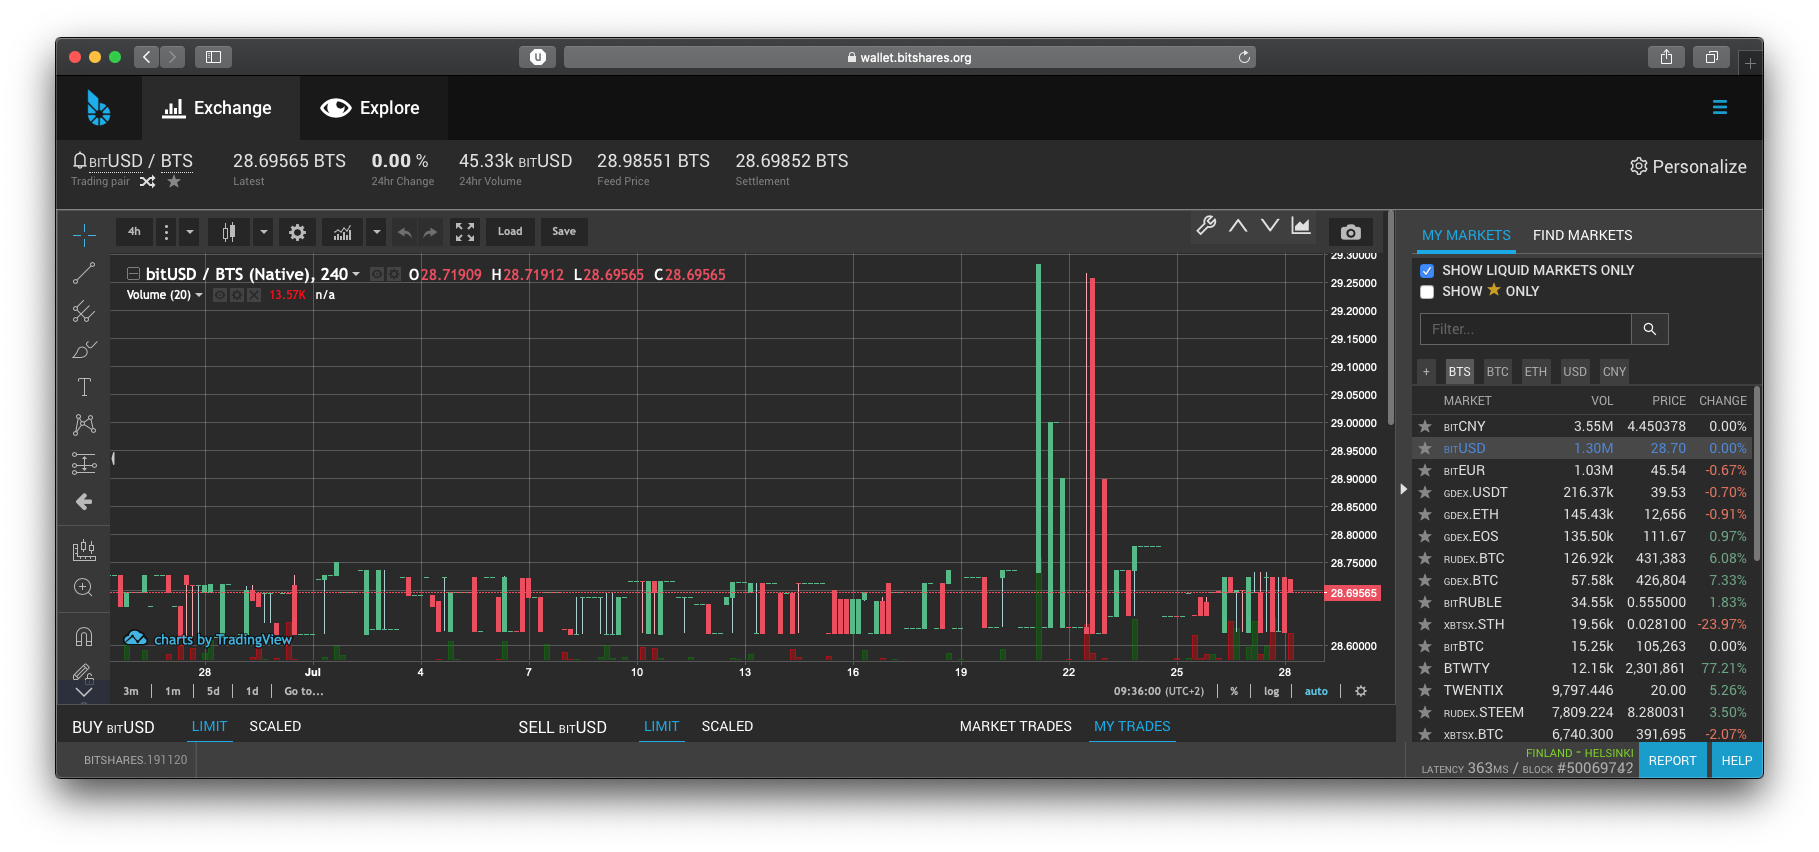
\includegraphics[width=\linewidth]{introduction/assets/bitshares}
	\caption{An online explorer provided by the BitShares DEX, showing recent and outstanding asset orders on the BitShares blockchain.}
	\label{fig:bitshares_explorer}
\end{figure}

\subsection{Decentralized Exchanges}
Blockchain technology is increasingly being used to build decentralized exchanges, also called \emph{DEXes}, to trade cryptocurrencies.
DEXes enable direct peer-to-peer trading without a market operator.
The first generation of DEXes limits trading to assets residing on the same blockchain.
On these DEXes, users can issue custom assets, transfer assets to others, and trade assets with other users by publishing buy and sell orders on the blockchain.
These orders are then automatically matched by miners during the validation of new transactions.
As we will further elaborate in Section~\ref{sec:matchmaking}, order matchmaking can also proceed outside the blockchain to increase efficiency, e.g., AirSwap~\cite{swap}.
Notable examples include Waves and BitShares which have accumulated a market capitalization of \$168 million and \$71 million dollars respectively at the time of writing.\footnote{https://coinmarketcap.com}
Figure~\ref{fig:bitshares_explorer} shows an online explorer of the BitShares blockchain, showing recent and outstanding asset orders.\footnote{https://wallet.bitshares.org}

We identify four advantages of DEXes over centralized cryptocurrency exchanges.
First, DEXes enhance security during the trading process; a trade is usually an atomic operation, and there is minimal risk of losing funds.
Second, users themselves remain in control of their funds when trading on a DEX and do not have to transfer ownership of their assets to the market operator.
Third, the transaction fees associated with trading on a DEX are usually lower compared to a centralized exchange since there is no profit-driven intermediary.
Forth, DEXes allow users to remain anonymous, whereas centralized exchanges often require the validation of one's identity.

Despite these advantages, many DEXes currently suffer from low liquidity and trading volume, making them less attractive for long-term trading.
Furthermore, their transaction throughput depends on the consensus model used by the underlying blockchain, which might make them unsuitable for bulk trading.
Finally, as DEXes are a relatively new technology, the user experience for traders can be perceived as overwhelming, in contrast to traditional exchanges which often provide a user-friendly trading interface.

\section{Disintermediation in Markets}
The popularity of electronic commerce has resulted in much interest to act as middlemen between buyers and sellers to benefit from their interactions~\cite{clark1999electronic}.
In many electronic markets, the role of matching buyers and sellers, and facilitating transactions is performed by a middlemen~\cite{bakos1998emerging}.
A well-known example is PayPal~\cite{paypal}, a payment service provider offering settlement services to customers buying goods from merchants.
PayPal not only process payments but it also acts as arbitrator when there a dispute between a buyer and seller arises.
The services of \emph{trusted intermediaries} such as PayPal is at the core of electronic market and ensures that a trade between a buyer and seller who might not necessarily trust each other proceeds without disputes.

Blockchain technology, and Bitcoin in particular, has challenged the need for trusted intermediaries.
In traditional payment systems, a financial institution acts as intermediary and handles payment between different (possibly foreign) banks.
Bitcoin has demonstrated that a decentralized system without financial institutions can be built, by leveraging cryptographic techniques.
Since the introduction of Bitcoin, there has been much effort by both industry and academia to critically look at the necessity of trusted intermediaries, and potentially replace them with another mechanism, e.g., smart contracts~\cite{lande2018sok}.
This process is also called \emph{disintermediation}.
Disintermediation usually lowers costs, since trusted intermediaries charge the involved traders for their services.
The process of disintermediation is tangential to the concept of decentralization (see Section X).
In particular, disintermediation requires decentralization as its foundation~\cite{guo2016blockchain}.

Disintermediation is a concept that pre-dates blockchain technology.
The Internet enabled quicker and convenient access to information, therefore opening opportunities to replace traditional broker agents~\cite{wigand2020whatever}.
A clear example of disintermediation can be found in the publishing market~\cite{giaglis1999disintermediation}.
Information technology enables book buyers to quickly place their order and authors to only print their books when there is actual demand.
This is also called printing-on-demand and removes the retailer from the traditional supply chain.

In many scenarios, it has been proven to be possible to disintermediate from a technical perspective.
Disintermediation is not always possible, nor desired.
However, in many scenarios there is a need to safeguard certain processes by intermediaries, in particular when considering the financial sector.
One might argue that electronic market require at least some intermediary to act as mediator between buyer and sellers if transactions are not atomic.
From a regulatory perspective, an intermediary can be required by law, e.g., when there is a need to verify the identify of new or existing business relations (this is also known as Know-your-Customer).

As also pointed out by other researchers, we argue that it is not likely that electronic markets will be fully disintermediated soon~\cite{zamani2018little}.
Rather than complete disintermediation, it is more likely that the role of existing intermediaries will be transformed.
For instance, financial institutions are currently exploring how distributed ledger technology can make their existing settlement services more efficient and reliable.
Perhaps the most influential solution, Corda, is currently being deployed by R3, a consortium consisting world's leading financial institutions~\cite{brown2016introducing}.
Another example is Ripple~\cite{armknecht2015ripple}, a credit network that is aimed to eventually replace the SWIFT payment infrastructure.
In practice, these solutions are not fully disintermediated since payments will still be processed by nodes operated by the involved financial institutions.


\section{Blockchain-based Marketplaces}
Given our definitions of decentralization and disintermediation in the context of electronic marketplaces, we now look how these concepts align with blockchain-based marketplaces.
Blockchain technology holds the promise to transform the market processes that currently require a trusted intermediary, e.g., when making payments to other peers.
It is important to clearly define what a blockchain-based marketplace means in the context of this work.
There is much confusion around the concept of blockchain-based marketplaces.
For example, the OpenBazaar market does not store its listings on a blockchain ledger but uses cryptocurrencies for peer-to-peer payments between merchants and customers.
In this work, \emph{a blockchain-based marketplace is a digital platform that leverages blockchain technology to carry out one or more of its critical operations}.

To better understand how this technology connects to existing market components, we describe the required components of blockchain-based marketplaces.
Figure~\ref{fig:electronic_markets} shows a decomposition of blockchain-based marketplaces.
This figure is the result of our literature survey where we have assessed both published and unpublished work on electronic marketplaces that use blockchain technology.
In general, we identify the following five mechanisms commonly used in blockchain-based marketplaces: \emph{matchmaking}, \emph{knowledge discovery}, \emph{settlement}, \emph{dispute resolution} and \emph{on-boarding}.
For each mechanism, we list approaches commonly found in the considered problem domain.
We now further discuss each identified mechanism. % the required components of blockchain-based marketplaces.

\begin{figure}[t]
	\centering
	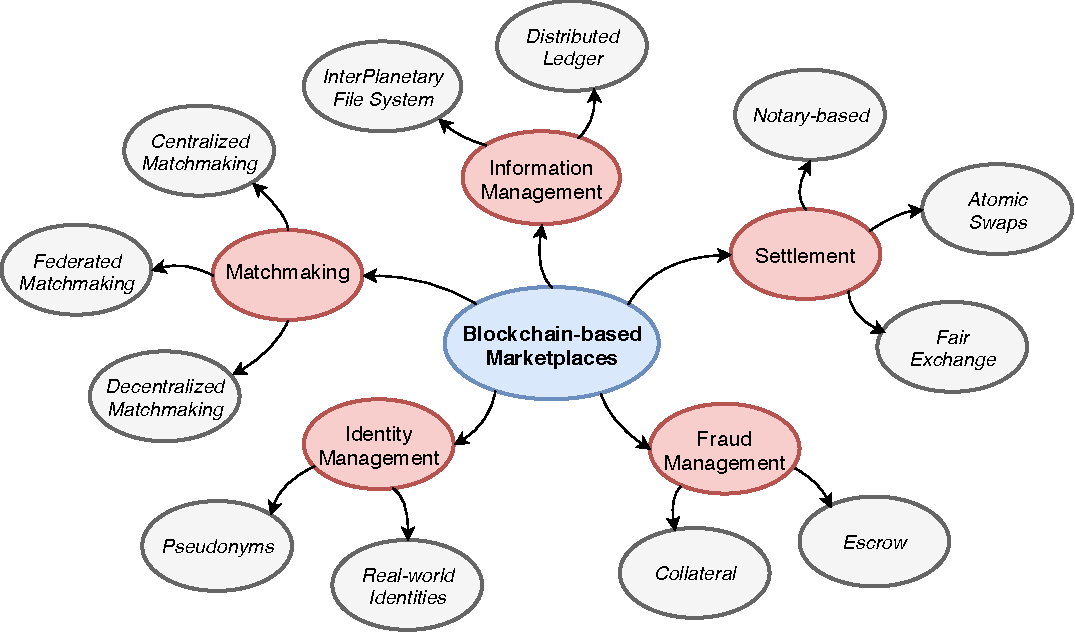
\includegraphics[width=\linewidth]{introduction/assets/decomposition}
	\caption{A decomposition of electronic marketplaces in four different components. Each component is further decomposed in approaches if applicable.}
	\label{fig:electronic_markets}
\end{figure}

\subsection{Knowledge Discovery}
Electronic marketplaces in general require a knowledge discovery mechanisms for market actors to enable value exchange.
Market knowledge includes pricing and product information, and details of past transactions.
Traditional electronic marketplaces usually store this information on centralized servers, deployed and managed by the market authority.
A key advantage of this approach for market operators is that these servers are relatively easy to setup and enable fast access to market information by participants.
Blockchain-based marketplaces usually avoid the storage of market information in a single location.
Therefore, market participants are dependent on others to retrieve the latest market state.

\subsubsection{Distributed Ledger}
A common approach for blockchain-based marketplaces is to store all available information on a distributed ledger.
This is, for example, the approach taken by DEXes like BitShares and Waves.
All market interactions are stored within tamper-proof transactions on a distributed ledger secured with global consensus.
Trades are either explicitly recorded in transactions, or can be derived from prior transactions.
Users wishing to get the latest market state are required to synchronize with the full distributed ledger from the network.
Since the distributed ledger might contain millions of transactions, some platform have setup a few \emph{full nodes} that remain synchronized in the network.
These full nodes offer an API that users can query to quickly retrieve market information.

\subsubsection{Order book}
A common market type is a financial exchange where financial instruments like currencies or bonds are being traded.
The buy and sell orders in these markets are usually bundled in an \emph{order book}.
An order book lists the specific assets or services that are being bought or sold within a market.
It provides traders with a convenient view on the current supply and demand.
Depending on the market and assets being traded, the order book sometimes reveals the identity of a trader behind an open order, or their reputation scores (for instance, Airbnb shows the reputation of hosts).
When presenting an order book to traders, ask and bid orders are usually sorted, i.e. based on their price.
For orders with a price, ask orders are sorted ascending on price in the order book and bid orders descending on price (the best orders are presented first).
%Market orders rarely end up in the order book as open order, since they are often fulfilled instantly.
%A defining metric used by traders is the difference between the price of the highest ask order and the price of the lowest bid order, also called the \emph{bid-ask spread}.
%For the order book shown in Figure \ref{fig:order_book}, the bid-ask spread is \$149.57 - \$149.54 = \$0.03.
%This metric also indicates market liquidity, the degree to which assets can be quickly bought or sold.
%A liquid market is often characterized by a low bid-ask spread.
The set of all ask or bid orders at a specific price is called a \emph{price level}.

\subsection{Settlement}
TODO

\subsubsection{Custodial}
A common approach to exchange blockchain-based assets is by using the services of a trusted intermediary.
A trade using a trusted intermediary completes as follows: two parties that agree on a trade transfer the assets for sale to one of the wallets owned by the trusted intermediary.
When this intermediary has received both assets, it finishes the exchange by transferring the appropriate assets to the other party.
In this approach, the trusted intermediary holds (temporary) ownership of the assets to be traded.
Relying on a trusted intermediary removes counterparty risk for the trading parties, but it requires both parties to have faith that the intermediary does not default or compromise their assets.

Trade through a trusted intermediary can facilitate value exchange between an extensive range of different blockchains, as long as the intermediary maintains wallets on the involved blockchains and can issue transactions in these systems to transfer the assets.
This is usually not an issue in permissionless blockchains since anyone can create accounts or wallets by generating a new cryptographic key pair.
Centralized cryptocurrency exchanges often facilitate asset trading across numerous permissionless blockchains.
Some cryptocurrency exchanges process transactions worth millions of dollars in total daily.\footnote{See https://coinmarketcap.com/rankings/exchanges}
In a permissioned blockchain environment, however, a trusted intermediary coordinating an asset exchange requires explicit approval from the operator to read and write transactions on the involved distributed ledgers.
Allowing new parties in a permissioned blockchain might be undesirable by operators since it introduces additional legal and operational risks.

\subsubsection{Atomic Swaps}
The \emph{atomic swap} is a distributed coordination task that allows asset exchange between different blockchains, without need for a trusted intermediary~\cite{herlihy2018atomic}.
Atomic swaps enable two parties to exchange blockchain-based assets with atomic guarantees: the asset exchange either completes or fails for both parties at any given time.
We now explain the involved operations during an atomic swap between the public Bitcoin and Ethereum blockchains.
Figure~\ref{fig:atomic_swap} visualizes the steps of an atomic swap between Alice and Bob, where Alice sells her Bitcoin in return for Ether (the native token of the Ethereum blockchain).
First, Alice generates a random secret $ s $ and computes $ H(s) $, where $ H(\cdot) $ denotes a hash function.
She then submits a hash-locked transaction, indicated by $ T_a(H(s)) $ (step \circled{1}), to the Bitcoin blockchain that transfers her Bitcoin to Bob's wallet address.
A hash-locked transaction is only executed when the secret $ s $ is provided to it.
Alice now sends $ H(s) $ to Bob (step \circled{2}).
Bob then submits a transaction $ T_b(H(s)) $ with the same hash lock to the Ethereum blockchain, transferring his Ethereum to the account of Alice (step \circled{3}).
Alice is now able to claim the assets held in custody by $ T_b(H(s)) $ (since she knows the value of $ s $), which in turn reveals $ s $ to Bob (step \circled{4}).
Bob now completes the swap by submitting $ s $ to the $ T_a(H(s)) $ transaction on the Bitcoin blockchain, which unlocks the assets in $ T_a(H(s)) $ (step \circled{5}).
To prevent the situation where assets are locked indefinitely if Alice refuses to reveal $ s $, Alice and Bob submit two additional time-locked transactions to ensure that assets in $ T_a(H(s)) $, respectively $ T_b(H(s)) $, can be claimed after some time $ t_1 $, respectively $ t_2 $.
To address the situation where Alice claims the assets in both $ T_a(H(s)) $ and $ T_b(H(s)) $, it must hold that $ t_1 > t_2 $.
These hash- and time-based agreements, also called Hashed Timelock Contracts (HTLCs), thus ensure trust-less, atomic asset exchange between trading parties, assuming that they claim the assets before the time-lock expires.
Atomic swaps eliminate the risk of losing assets to an adversarial trader while trading.
The HTLC atomic swap requires a total of four transactions.

\subsubsection{Notary-based}
Notary schemes are another solution for asset exchange where approval by a group of credible nodes (notaries) is required to perform some operation.
Notary schemes aim to partially alleviate the trust issues arising when relying on a single trusted intermediary through the approval by a group of semi-trusted notaries instead.
These notaries reach consensus on the occurrence of particular events, e.g., on the inclusion of a transaction on a distributed ledger.
Compared to an asset exchange through a trusted intermediary, notary schemes assume a weaker trust model and can often withstand adversarial behavior of a fraction of the notaries.

The Interledger project, introduced by Ripple, is the most advanced approach in this direction~\cite{thomas2015protocol}.
Interledger proposes a notary-based protocol to conduct payments across different ledgers.
In atomic mode, these payments are realized through atomic swaps and are coordinated by a different group of notaries for every involved blockchain.
Interledger uses payment paths where additional intermediate platforms and their notaries are used to exchange assets between ledgers that do not have a direct connection.
Interledger also supports bidirectional asset exchange but is vulnerable to a fraction of notaries colluding with one of the trading parties.
External coordination is avoided in universal mode, which relies on incentives for participants to behave honestly and not to commit fraud.
The Hyperledger Quilt project provides a Java implementation of the Interledger protocol for permissioned blockchains~\cite{hyperledgerquilt}.

\subsubsection{Fair Exchange}
TODO

\begin{figure*}[t]
	\centering
	\begin{subfigure}[t]{.33\textwidth}
		\centering
		\captionsetup{width=.9\linewidth}
		\includegraphics[width=.9\linewidth]{introduction/assets/centralized_matchmaking}
		\caption{\emph{Centralized matchmaking}: new orders are always sent to a single matchmaker, usually a centralized system (server).}
		\label{fig:centralized_matchmaking}
	\end{subfigure}%
	\begin{subfigure}[t]{.33\textwidth}
		\centering
		\captionsetup{width=.9\linewidth}
		\includegraphics[width=.9\linewidth]{introduction/assets/federated_matchmaking}
		\caption{\emph{Federated matchmaking}: new orders are sent to one of the available matchmakers in the network.}
		\label{fig:federated_matchmaking}
	\end{subfigure}%
	\begin{subfigure}[t]{.33\textwidth}
		\centering
		\captionsetup{width=.9\linewidth}
		\includegraphics[width=.9\linewidth]{introduction/assets/decentralized_matchmaking}
		\caption{\emph{Decentralized matchmaking} (our proposal): new orders are sent to multiple matchmakers and shared between them.}
		\label{fig:decentralized_matchmaking}
	\end{subfigure}
	\caption{Three models for order matching. Traders create offers and requests (colored green and red respectively), which are matched by matchmakers (depicted in blue).}
	\label{fig:matching_models}
\end{figure*}

\subsection{Order Matchmaking}
\label{sec:matchmaking}
Automatically \emph{matching} customers is a prerequisite for online trade and therefore essential for electronic marketplaces.
Matchmaking is defined as the process of mediating supply and demand in markets, based on profile information~\cite{Veit:2003fs}\footnote{In multi-agent systems, a matchmaker is considered as an entity that only aggregates offers. Brokers aggregate both offers and requests. We will use the term matchmaker in this paper since we found it to be more common in related work.}.
Notable examples are matching idle agents to incoming jobs or matching suppliers of specific assets to consumers who are interested in buying these assets.
Inefficient matchmaking between participants decreases overall market efficiency and customer satisfaction~\cite{Wu2015TheM}.
%For example, in a ride-hailing marketplace like Uber, it is key to match nearby drivers and passengers in a timely and efficient manner.
For instance, prolonged suboptimal matching by ride-hailing marketplaces such as Uber increases the waiting time for passengers and results in drivers having to traverse a greater distance to pick up their customers.
%Similarly, inefficient matching of available computer resources to customers by cloud providers could violate service-level agreements, resulting in customer loss and reputational damage.

In this section, we review different approaches to order matchmaking in electronic markets.
Matchmaking depends on the individual constraints and preferences of market participants.
In most electronic markets, a participant includes this information in an \emph{order} that indicates their intention to buy and sell assets, resources, or services~\cite{Veit:2003fs}.
This order is then submitted to a matchmaker.
In general, economic literature distinguishes between two types of orders: \emph{asks}, created by traders offering a specific asset, service, or resource, and \emph{bids}, created by interested buyers.
%Each order can have multiple attributes attached, e.g., a price or a location.
The main objective of a matchmaker is a quick and effective mediation between incoming offers and requests, based on constraints and preferences included in each order.

We identify three different approaches to order matchmaking, depicted in Figure~\ref{fig:matching_models}.
With \emph{centralized matchmaking} (Figure~\ref{fig:centralized_matchmaking}), traders submit their asks and bids to a single server.
With \emph{federated matchmaking} (Figure~\ref{fig:federated_matchmaking}), traders submit a new order to one of the servers of their choice.
Finally, in \emph{decentralized matchmaking} (Figure~\ref{fig:decentralized_matchmaking}), traders submit their orders to one or more matchmakers.
We further elaborate on each matchmaking model.

\subsubsection{Centralized Matchmaking}
Figure~\ref{fig:centralized_matchmaking} visualizes the centralized matchmaking model, which is the most common approach to match orders.
Traders send new offers and requests to a dedicated matchmaker, usually a centralized system (server).
This model is widely adopted by commercialized marketplaces such as stock exchanges or peer-to-peer service markets like Uber.
A matchmaker bundles open orders in a local data structure known as an \emph{order book}.
The order book stores all active asks and bids, and provide traders a convenient view on the current supply and demand.
A new incoming ask or bid is then matched with other bids and asks, respectively, using a \emph{matching policy}.
The most common matching policy used in cryptocurrency exchanges is the \emph{price-time} strategy, where orders are first matched based on the price, and then on their order creation time (older orders are prioritized).
The order book is often optimized for fast order lookup and matching within a specific trading domain.

The EtherDelta decentralized exchange is one of the first DEXes that adopt the centralized matchmaking model~\cite{Anonymous:brZbAflS}.
EtherDelta maintains a single server that stores an order book with all active orders.
Traders can browse the order book and trade against orders in the order book.
The trades are finalized on the blockchain, and the order is then removed from the EtherDelta order book.\todo{custodial vs non-custodial}
The IDEX exchange also deploys a centralized server but automatically matches orders submitted by makers and takers~\cite{AuroraLabs:B4jmyRY8}.
Specifically, traders lock their assets in the IDEX smart contract and submit their order to the IDEX server, which checks its validity.
The order is then executed by the Ethereum smart contract and the order book is updated according to the executed trade.

A main advantage is that the centralized matchmaking model with a single server is relatively straightforward to implement, since no communication or order book synchronization is required.
Also, since all orders are stored and matched by single matchmaker, orders are processed based on full market knowledge.
The identity behind each order is only known to the market operator, therefore protecting the privacy of individual traders.

Unfortunately, the emergence of electronic trading in general gave rise to fairness, transparency and manipulation issues during the matchmaking process~\cite{Mavroudis:2019iw}.
For example, the EtherDelta operator is able to censor specific orders.
Furthermore, information asymmetry between exchange operators and traders allows operators to front-run specific orders (see Section X\todo{x}).
The work of Mavroudis and Melton address fairness issues arising from the latency traders experience when submitting orders and gaining market information~\cite{Mavroudis:2019iw}.
They propose Libra, an order reordering matching policy that alleviates the effects of uneven delays by the market infrastructure.
Libra remains temporally fair, meaning that among all pairs of participants on it the probability that a slower participant succeeds in capturing a trading opportunity at the expense of a faster participant (who, responsive to the same stimulus, is also competing for the same opportunity) does not exceed 0.5.

From a systems perspective, centralized matchmaking has a low scalability compared to distributed solutions since the matchmaker becomes a bottleneck when more orders are created in the same time period.
Fault tolerance is another concern: if the single matchmaker becomes unavailable, e.g., due to infrastructure failures, incoming orders cannot be matched and all market activity stalls.

\subsubsection{Federated Matchmaking}
Figure \ref{fig:federated_matchmaking} illustrates an alternative model for order matching: federated matchmaking.
Instead of relying on a central matchmaker, multiple (independent) matchmakers individually maintain an order book.
The group of matchmakers can either be static (e.g., elected by a committee or a voting mechanism), or dynamic (e.g., each peer can opt-in to become a matchmaker).
A trader now submits new orders to their preferred matchmaker (for example, based on the reliability or trustworthiness of individual matchmakers).
The 0x and Swap protocols are notable examples of the federated matchmaking model and are discussed next.

%Blockchain-powered marketplaces based on the 0x and AirSwap protocols have adopted the federated matchmaking model~\cite{warren20170x}~\cite{oved2017swap}.
The 0x protocol uses off-chain order relaying and on-chain settlement, meaning that orders are created shared, and matched outside a blockchain.
A maker creates market liquidity in 0x by first selecting an available relayer.
Each relayer maintains an off-chain order book and charges a transaction fee for its services.
The maker then creates the order and specifies a fee which is given by the selected relayer.
Takers query the order book of relayers and if they intend to fulfill an order, they submit it to the Ethereum blockchain.
The Augur prediction market (see Section~\ref{sec:prediction_markets}) leverages the 0x protocol for order dissemination and matching.

The Swap protocol follows a similar off-chain matchmaking, on-chain settlement model~\cite{oved2017swap}.
In Swap, indexers aggregate trade intents created by market makers and takers.
The indexer informs takers when a matching trade intent has been found, upon which a peer-to-peer negotiation process starts between the matched maker and taker.
During this negotation process, a maker may contact an oracle to get a price suggestion.
When a maker and taker agree on a trade, the taker submits the agreement to an Ethereum smart contract, upon which the trade is executed and on-chain assets are exchanged.
We remark that both 0x and Swap are limited to trading Ethereum-based digital tokens and can therefore not be used for order processing of any blockchain-based asset.

The federated matchmaking model gives traders the opportunity to use the services of their preferred matchmaker.
Manipulative behaviour of one matchmaker then leads to the situation where traders select another, honest matchmaker.
Furthermore, unavailability of an individual matchmaker is less likely to stall all market activity since a trader can send their orders to another available matchmaker.
However, the order book is fragmented across different matchmakers, potentially leading to less market efficiency and liquidity, compared to matchmaking with an order book managed by a single entity.

\subsubsection{Decentralized Matchmaking}
%Scalability limitations, low fault tolerance, and uneven load balancing are inherent issues of centralized and federated matchmaking.
The \emph{decentralized matchmaking} model is depicted in Figure \ref{fig:decentralized_matchmaking}.
The main idea is that a single order is sent to multiple matchmakers simultaneously and matchmakers share their orders with other matchmakers (liquidity sharing).
We distinguish between on-chain and off-chain decentralized matchmaking.

\textbf{On-chain.}
We now discuss on-chain matchmaking approaches that either rely on a smart contract to match incoming orders, or embed the matchmaking logic in the transaction validation logic.
The Stellar protocol integrates DEX functionality that enables users to create buy and sell orders that trade assets native to the Stellar ledger~\cite{Lokhava:2019kd}.
These orders are created using specific transaction types, that are matched with existing, outstanding orders during inclusion of the transaction in the ledger.
The Stellar matching engine uses the price-time policy.
Similarly, the BitShares blockchain provides functionality to create orders at the protocol level~\cite{Schuh:CsvWDxUZ}.

The main advantage of on-chain matchmaking is tight integration with the blockchain platform; no external components such as a peer-to-peer overlay are needed to process orders.
Instead, all orders can simply be processed by the blockchain logic.
This also makes it more convenient for users to submit their orders.
On the other hand, since users likely need to pay transaction fees when creating new orders or when cancelling existing ones, trading in bulk can become a costly process.
Furthermore, blockchain-based order matching can be orders of magnitude slower compared to centralized matchmaking, due to security requirements.
Finally, on-chain matching protocols do not explicitly store the history of matches.
Therefore, the reconstruct the order book at a specific block height, one needs to process all transactions up to that point.

\textbf{Off-chain.}
To overcome transaction fees and slow transaction confirmation times, some platforms maintain a fully decentralized order book off-chain.
An example of off-chain decentralized matchmaking is the Loopring protocol, which builds a decentralized order sharing protocol~\cite{Wang:wt}.
Loopring is able to mix and match multiple orders in circular trade, also called order rings, therefore increasing liquidity.
New orders are sent to one or more relays in a mesh network.
Order rings are submitted to a smart contract, e.g., on Ethereum, where the trade is then executed.
Relayers can optionally share orders with other relayers to increase liquidity, however, the whitepaper lacks technical details on how this is achieved specifically.
Relayers take the margin between two matched orders, or can charge some fee.
% front-running in Loopring

The Republic Protocol builds a decentralized network of nodes that match orders without revealing any information about individual orders~\cite{Zhang:kGvi0me4}.
Specifically, it uses Shamir Secret Sharing to break down an order in multiple order fragments which are distributed through the network.
An Ethereum smart contract, called the Registrar, describes the network topology such that it is hard for an adversary to fully reconstruct an original order.
Nodes cooperate with other nodes to check if their order fragments match, by computing a zero-knowledge proof.
When two order fragment match, an atomic swap is initiated between the two traders (also see Section~\ref{sec:atomic_swap}).
Note that this prevents an individual from estimating the total liquidity in the network.

We identify two advantages of this model over centralized and federated matchmaking.
First, sharing orders between matchmakers can yield the same matching effectiveness compared to centralized matchmaking, depending on the order synchronization details. %since orders can be synchronized amongst matchmakers.
Second, decentralized matchmaking should show higher tolerance against failure of individual matchmakers.
However, this model increases bandwidth usage since orders are sent to multiple matchmakers.
Also, it might take longer before a new order is fulfilled in the case that it is sent to matchmakers that are unable to match this order immediately.

\subsection{Identity Management}
Identity management is a key component of any electronic market.
Traditional electronic marketplaces usually impose some form of identity validation before a user is allowed to engage in trade with other users.
In this situation, the digital identity is linked to real-world credentials, e.g., a passport.
Identity validation in electronic marketplaces has several purposes.
First, it adds accountability of ones actions within the market in case of a dispute between a buyer and seller.
Second, it prevents the situation where a user can easily re-enter the market under a different identity after having committed fraud.
Third, identity verification is often part of the regulatory compliance of market operators, as often required by anti-money laundering policies.
Most cryptocurrency exchanges managed by a central market authority require users to verify their identity before they can create buy or sell orders.

In stark contrast with traditional marketplaces, a key property of blockchain technology is the ability to join the network under a pseudonym, using a locally generated cryptological keypair.
In Bitcoin, for example, users can easily transfer Bitcoin to others using different digital identities.
This is even the preferred practice when one wants to retain anonymity in the Bitcoin network.
Similarly, many DEXes do not require identity verifications and allow traders to join the network under a pseudonym.

\subsection{Fraud Management}
Fraud is a key concern in electronic marketplaces.
A common type of fraud is \emph{counterparty fraud}, where a party does not fulfil its obligation towards the counterparty during trade settlement, e.g., by not delivering the promised assets or goods.
This kind of fraud is often resolved by the market operator, acting as arbitrator during the dispute resolution process.
Within blockchain-based marketplaces, counterparty fraud is often prevented since asset exchange is atomic: either all parties receive their assets or nothing happens.
This approach works when assets can be exchanged directly, e.g., on a blockchain-powered DEX.
Fraud management, however, is required when settlement depends on the actions by users.
We identify different approaches to manage fraud.

\subsubsection{Escrows}
TODO

\subsubsection{Collateral}
Some blockchain-based marketplaces require users to deposit collateral before trading.
This collateral is slashed when its depositor does not adhere to an agreement and therefore incentivise traders to follow the protocol.
The XClaim protocol relies on collateral deposits to enable asset trading between distinct blockchain ledgers.
When a participant deviates from the protocol, the collateral is slashed and wronged actors are reimbursed.

%\section{Problem Statement}
%The key issue is that decentralized applications that are using blockchain technology are often not scalable enough.

\section{Research Questions}
In this thesis, we mainly focus on \emph{knowledge discovery}, \emph{matchmaking} and \emph{settlement} in electronic markets.

The overarching research question of this thesis is as follows:\\\\
\emph{How can we improve matchmaking and settlement mechanisms in blockchain-based marketplaces?}\\\\
To answer our research question, we address the following key questions:

\textbf{[RQ1] What is the state-of-the-art in blockchain-based electronic trading and asset exchange?}
To provide an answer to our research question, it is required to build an understanding of state-of-the-art approaches to blockchain-based trading, and their shortcomings.
Even though there is much active research on blockchain-based decentralized exchanges and secure asset trading between heterogeneous blockchain platforms, the field lacks a systematic literature overview, an analysis of open challenges and suggestions for further research.

\textbf{[RQ2] How can we efficiently match market orders without centralized coordinator?}
The predominant approach to order matchmaking in electronic markets is by using a centralized server, owned by the market operator.
This approach, however, enables manipulation by the operator, resulting in an unfair system.
Blockchain-based matchmaking has the potential to address fairness issues but is by far not scalable enough for usage by many marketplaces.
We aim for an efficient matchmaking mechanism with fairness guarantees, not under the control of a single market operator.

\textbf{[RQ3] How can improve settlement durations of (international) payment infrastructures?}
A major problem of current banking systems is that the settlement duration of a payment between two different (international) banks is significant, often in the order of days.
Furthermore, these payments require significant transaction fees to cover back-office costs.
Blockchain technology holds the potential to improve the speed of (international) payment infrastructures, and potentially lead to a reduction of costs and lower transaction fees.

\textbf{[RQ4] How can we exchange assets managed by different blockchains?}
Decentralized exchanges (DEXes) is a new type of decentralized application where digital assets are issued and traded on a blockchain.
Compared to centralized exchanges, DEXes take a non-custodial approach where users manage these assets themselves.
The main issue, however, is that the assets on a specific DEX are locked to a single blockchain; trade between different DEXes is either impossible or slow.
The question is how to address these issues and enable fast asset trading between different exchanges.

\textbf{[RQ5] How can we apply blockchain technology to improve software crowdsourcing markets?}
The engineering of blockchain-based applications such as exchanges is a challenging task and requires engineers with appropriate qualifications.
Crowdsourcing is a relatively new model for software development, where an open call is made for the documentation, design, coding, and testing of software.
Recent research proposes to leverage blockchain technology
Applying accountability and fraud detection could improve the software crowdsourcing process.

\begin{table*}[t]
	\small
	\centering
	\begin{tabular}{ |c|c|c|c| }
		\hline
		\textbf{Chapter} & \textbf{Mechanism} & \textbf{DAS5 experiments?} & \textbf{Deployment?} \\ \hline
		2 & TrustChain & yes & yes, integration in Tribler \\ \hline
		3 & MATCH & yes & yes, integration in Tribler \\ \hline
		4 & XChange & yes & yes, integration in Tribler \\ \hline
		5 & Internet-of-Money & yes & in-house testing \\ \hline
		6 & DevID & no & user trial \\ \hline
	\end{tabular}
	\caption{An overview of research methods for each mechanism introduced in this thesis.}
	\label{table:research_methodology}
\end{table*}

\section{Research and Engineering Methodology}
Blockchain technology is a relatively new and immature field.
We identify two fundamentally different approaches to the adopted research methodology in this field.
On one hand, published blockchain research in systems-oriented conferences follow an experimental methodology where the performance of the proposed mechanism is systematically evaluated using a comprehensive set of experiments and benchmarks.
On the other hand, there is a vast body of research on the security aspects of distributed ledgers.
This kind of research tend to follow a more theoretical approach through the use of formal proofs or small-scale protocol simulations.

In this work, we adopt an experimental-driven approach where we answer each research question by designing, implementing and evaluating a system or mechanism.
We then systematically evaluate the appropriate properties of each mechanism, and if feasible, we deploy our mechanisms to users to gather real-world results.
For all of our proposed mechanisms, we aspire a practical solution, ready for deployment and usable by real users.

Distributed systems can be complex software implementations with many components that work together.
Specifying the scope of a system is a non-trivial challenge and failing to implement clear system boundaries can result in numerous performance bottlenecks and degradation of user experience when such a system is deployed.
To this end, during the design of each mechanism we specify the boundaries of each system and state what we consider out of scope.
We aim to focus on the core functionality of each mechanism.

Table~\ref{table:research_methodology} specifies for each mechanism whether we present a set of DAS5 experiments and/or whether we have conducted a real-world deployment.
Except for DevID, we evaluate each component using a comprehensive set of experiments that have been conducted on our DAS5 nation-wide compute cluster.

Driven by our focus on practicality, we have deployed each mechanism proposed in this thesis, either to a small group of users or with an integration in Tribler.
Tribler is our academic testbed and offers decentralized, anonymous file-sharing capabilities.
Tribler has been downloaded by over 1.5 million users and enables us to test our ideas in a geo-distributed, real-world environment.
We have evaluated TrustChain, for example, in the context of our anonymous file-sharing overlay to address free-riding behaviour.
This longitudinal deployment allowed us to incrementally improve our software and refine our ideas.
Due to legal considerations, we have been unable to provide an open-source implementation of the Internet-of-Money mechanism.

We ensure that each mechanism is tested.
Even though this is uncommon practice for research projects, we believe that a proper engineering methodology adds credibility to the presented mechanisms, helps reproducibility and is instrumental in getting a system ready for deployment.

% simplicity?

%We believe this experimental research methodology is suitable for two reasons.
%First, it allows us to evaluate our ideas in an environment that closely resembles a real-world environment.
%Second, it directly leads to a software implementation that can be used by academia or industry.
%All developed software artefacts are available on our GitHub repository and contain unit tests to verify functional correctness.

% existing research does X

% but we do Y!

\begin{figure}[t]
	\centering
	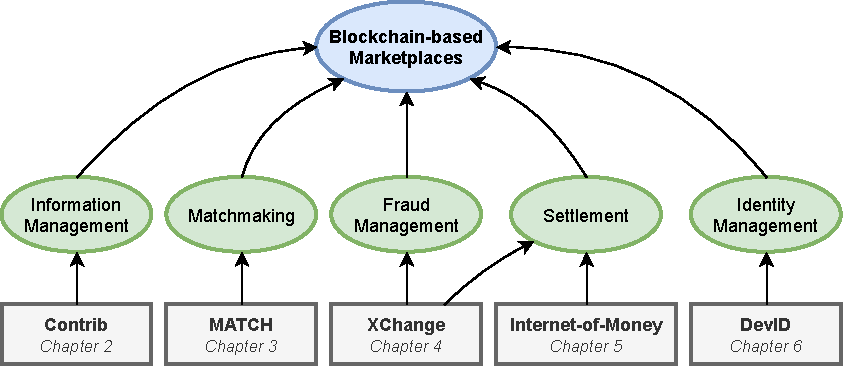
\includegraphics[width=\linewidth]{introduction/assets/thesis_overview}
	\caption{The five mechanisms presented in this work (depicted in grey), in the context of blockchain-based marketplaces and their components.}
	\label{fig:thesis_overview}
\end{figure}

\section{Contributions and Thesis Outline}
After establishing the required background on decentralized applications and distributed ledger technology, Chapter \todo{X} highlights scalability limitations of state-of-the-art blockchain ledgers.
Next, in Chapter \todo{X}, we design, implement and evaluate TrustChain: a scalable blockchain ledger that is based on fraud \emph{detection} instead of fraud \emph{prevention}.
In Chapters \todo{X to Y}, we apply accountability primitives and fraud detection techniques in three well-established domains: financial transactions, two-sided marketplaces, and identity.
Specifically, we make the following contributions in each chapter:\\

\textbf{[Chapter 2] SoK: Electronic Markets in the Age of Blockchain.} (Work in progress)
In this chapter, we answer RQ2 and provide an extensive overview of existing approaches for online trade in the age of blockchain.\\

\todo{Work in progress}\\

\textbf{[Chapter 3] MATCH: Accountable and Generic Matchmaking for Decentralized Applications.}
In this chapter, we partially address RQ4 and focus on matchmaking, the process of bringing market participants together based on individual preferences.
Matchmaking is a cardinal, yet overlooked prerequisite for a fully decentralized exchange.
Although numerous companies have deployed infrastructure for matchmaking, there is currently no solution that can be deployed within different trading domains.
We present MATCH, a middleware for generic order matching.
Since MATCH is agnostic about order specifications, the resulting system is highly flexible and reusable.
In this work, we first present an alternative approach to order matching, named \emph{decentralized matchmaking}.
The main idea is that new orders are disseminated to multiple matchmakers simultaneously and shared between matchmakers.
We then design and implement a novel matching protocol and a middleware with full support for both existing matchmaking paradigms and decentralized matchmaking.
Finally, we extensively evaluate desired system properties of MATCH under a real-world ride-hailing and asset trading workload.
Our main finding is that decentralized matchmaking exhibits superior fault tolerance and load balancing, at the cost of moderately increased bandwidth usage and order completion time.
This chapter is based on the following publication:

\todo{UNDER REVIEW}\\

\textbf{[Chapter 4] XChange: A Scalable Asset Marketplace based on Accountability.}
In this chapter, we answer RQ4 and introduce XChange, an asset marketplace based on accountability guarantees.
There is an increasing need for a generic mechanism to trade assets across isolated platforms, as more industries rely on the digital management of their physical resources using Internet-of-Things devices.
To date, there is no such mechanism without dependency on a trusted third party.
We address this shortcoming and present XChange, a blockchain-based mechanism for generic asset trading.
Unlike existing asset trading marketplaces, we decouple trade management and the actual exchange of assets.
XChange enables the trustworthy trade of \emph{any} digital asset.
We describe a generic trading protocol that establishes trade between individuals and accounts market activity on any distributed ledger.
We prove with a theoretical analysis that the effectiveness of fraud conducted by adversarial parties is limited.
Furthermore, we devise a novel market architecture, composed of all required components for a decentralized asset marketplace.
We implement the XChange mechanism and conduct real-world evaluations.
To account market activity in a tamper-proof manner, we use an existing scalable blockchain ledger, TrustChain.
By deploying XChange on multiple low-resource devices, we show that a full trade can be completed within 500 milliseconds.
To analyze the scalability and bandwidth usage, we conduct further experiments on our compute cluster and deploy up to 500 XChange instances.
Our main finding is that the throughput of XChange, in terms of trades per second, scales linearly with the network size.
This chapter is based on the following publication:

\todo{UNDER REVIEW}\\

\textbf{[Chapter 5] Internet-of-Money: Applying Accountability to Enable Real-time International Money Transfers.}
In this chapter, we answer RQ3 and explore a new stage in the evolution of digital trust, trusting strangers with your money.
We address the challenging problem of giving money to others and relying on them to forward it.
To identity fraud, we account money transfers between interacting strangers.
This work represents a small step towards a generic infrastructure for trust, moving beyond proven, single-vendor platforms like eBay, Uber and AirBnb.
Expanding upon trust relations, we designed, implemented and evaluated an overlay network: \emph{Internet-of-Money}.
Internet-of-Money is capable of real-time money transfers to different banks by routing funds through individuals (\emph{money routers}).
This removes the need for central banks to handle a payment.
Our network reduces traditional payment durations from a day or even a few days in weekends, to mere seconds.
%Internet-of-Money is fully decentralized, privacy-preserving and highly scalable.
With real-world experimentations, we prove that Internet-of-Money enables fast money forwarding.
We show that our overlay network is capable of discovering a majority of available money routers within a minute.
Finally, we demonstrate how profit of cheating routers is limited and that misbehaviour is punished.
This chapter is based on the following publication:

Martijn de Vos and Johan Pouwelse, \enquote{Real-time Money Routing by Trusting Strangers with your Funds}, \emph{IFIP Networking, 2018.}\\

\textbf{[Chapter 6] DevID: Blockchain-based Portfolios for Software Developers.}
In this chapter, we answer RQ5.
Decentralized applications, also known as dApps, are the new paradigm for writing business-critical software.
Recruiting developers with appropriate qualifications and skills for this activity is key, yet challenging.
The main problem is that the portfolio of developers is usually scattered across centralized platforms like GitHub and LinkedIn, and vendor locked.
This can result in an incomplete impression of their capabilities.
We address this problem and introduce \emph{DevID}, a blockchain-based portfolio for developers.
Over time, this portfolio enables developers to build up a trustworthy collection of records that showcase their capabilities and expertise.
They can import data assets from third parties into a unified DevID portfolio, add projects and skills, and receive endorsements.
All portfolio records are stored on a scalable distributed ledger and owned by developers themselves.
The essential idea is to exploit the tamper-proof property of the blockchain while providing durable storage.
To demonstrate the practical value of DevID, we build the competition-based platform, \emph{dAppCoder}, for the development of decentralized applications.
On dAppCoder clients are able to submit their ideas and developers can find work.
dAppCoder utilizes DevID portfolios to match these clients and developers.
We fully implement our ideas and conduct a deployment trial.
Our trial demonstrates that DevID is efficient at storing portfolio records.
This chapter is based on the following publication:

Martijn de Vos, Mitchell Olsthoorn and Johan Pouwelse, \enquote{DevID: Blockchain-based Portfolios for Software Developers}, \emph{IEEE International Conference on Decentralized Applications and Infrastructures (DAPPCON'19)}\\

\textbf{[Chapter 7] Conclusion.} We will end this thesis with the conclusion, a summary of the lessons learned, and suggestions for further work.

%\begin{figure}[t]
%	\centering
%	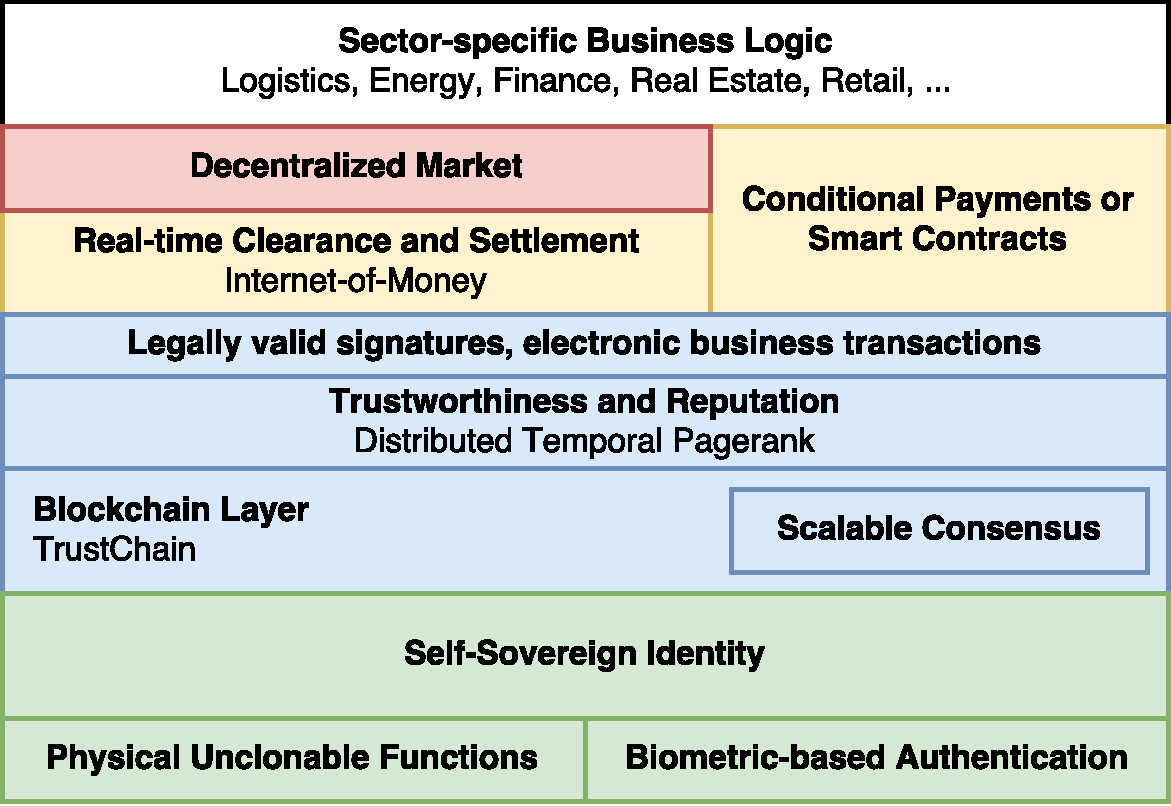
\includegraphics[width=.7\linewidth]{introduction/assets/tech_stack}
%	\caption{An overview of the research conducted at the Delft Blockchain Lab.}
%	\label{fig:dbl_tech_stack}
%\end{figure}

%\section{About the Delft Blockchain Lab}
%The Delft Blockchain lab is Delft's initiative for research, education and training in blockchain technology and trust on the Internet.
%Figure~\ref{fig:dbl_tech_stack} outlines the research directions of the Delft Blockchain Lab, ranging from low-level primitives like biometric-based authentication to sector-specific business logic.
%At the lowest layers (depicted in green), we build, deploy and evaluate new solutions for managing ones identity in the physical world and on the Internet.
%These solutions include biometric-based authentication and physical unclonable functions, a method to securely store a private key.
%A part of our ongoing research includes a self-sovereign identity solution that is currently being tested and deployed in the Netherlands.

%Our research effort around distributed ledger technology includes scalable consensus algorithms and Sybil-resistant reputation mechanisms.
%The TrustChain distributed ledger is presented in Chapter X.
%The other components of this thesis are mostly focussed on the research directions that are coloured yellow and red in Figure~\ref{fig:dbl_tech_stack}.
%For a detailed outline of our research efforts, we refer the reader to our published vision paper.

%\newpage

%\bibliographystyle{unsrt}
%\bibliography{introduction}

\chapter{ConTrib: Maintaining Fairness in Decentralized Big Tech Alternatives by Accounting Work}
\label{chapter:trustchain}

\emph{\enquote{Big Tech} companies provide digital services used by billions of people.
Recent developments, however, have shown that these companies often abuse their unprecedented market dominance for selfish interests.
Meanwhile, decentralized applications without central authority are gaining traction.
Decentralized applications critically depend on its users working together.
Ensuring that users do not consume too many resources without reciprocating is a crucial requirement for the sustainability of such applications.}

\emph{We present \ModelName{}, a universal mechanism to maintain fairness in decentralized applications by accounting the work performed by peers.
In \ModelName{}, participants maintain a personal ledger with tamper-evident records.
A record describes some work performed by a peer and links to other records.
Fraud in \ModelName{} occurs when a peer illegitimately modifies one of the records in its personal ledger.
This is detected through the continuous exchange of random records between peers and by verifying the consistency of incoming records against known ones.
Our simple fraud detection algorithm is highly scalable, tolerates significant packet loss, and exhibits relatively low fraud detection times.
We experimentally show that fraud is detected within seconds and with low bandwidth requirements.
To demonstrate the applicability of our work, we deploy \ModelName{} in the \Tribler{} file-sharing application and successfully address free-riding behaviour.
This two-year trial has resulted in over \TrialRecords{} records, created by more than \TrialUsers{} users.}

\newpage

\section{Introduction}

Over the last decades, \enquote{Big Tech} companies have obtained an unprecedented market dominance in the industry for information technology~\cite{frost2019bigtech}.
Companies such as Google, Amazon, Facebook, and Apple are omnipresent in our current society and even have the means of acting as small states, inhabited by billions of users worldwide.
By continuously broadening their activities, these companies seek to expand their virtual territory and seek to obtain monopolistic control over the enabling elements for digital services, such as access to the Internet~\cite{best2014internet}.

The societal impact of \enquote{Big Tech} companies is a double-edged sword.
On the one hand, these companies are facilitating new modes of digital interaction between users and enable new business models.
The sharing economy is a prime example of this phenomena.
It is made up by digital markets for the trustworthy exchange of personal assets (e.g., houses and cars) between strangers~\cite{schor2016debating}.
Sharing personal assets is a concept that has long been confined to trusted individuals, such as family and friends~\cite{frenken2019putting}.
Likewise, media platforms such as YouTube provide the required infrastructure for new forms of user engagement through video weblogging or \enquote{vlogging}.

On the other hand, it has become apparent that \enquote{Big Tech} companies tend to exploit their established market position and are increasingly involved in regulatory or political battles.
This behaviour sometimes goes undetected for years.
For example, researchers have only recently demonstrated that Uber actively manipulates the matchmaking process between passengers and drivers for commercial interests, therefore decreasing platform fairness and income equality of drivers~\cite{bokanyi2019ride}.
Similarly, Apple is currently under antitrust investigation by the European Commission that is assessing whether Apples' rules for developers on the distribution of apps via the App Store violate competition rules~\cite{kotapati2020antitrust}.

These concerning developments have contributed to an increase in the deployment of \emph{decentralized} applications.
Decentralized applications avoid centralized ownership and delegate the decision making away from a single authority.
A decentralized application mainly operates through the direct cooperation and information exchange between users, which we call \emph{peers}.
Arguably, Bitcoin is the most influential solution in this direction and provides a decentralized cash system without the supervision by an authoritative bank~\cite{nakamoto2019bitcoin}.
The underlying data structure of Bitcoin, a blockchain, is at the core of numerous decentralized applications~\cite{bashir2018mastering}.
At the time of writing, there are thousands of decentralized applications deployed on the Ethereum blockchain alone~\cite{wood2014ethereum}.
These decentralized applications include marketplaces, auctions, voting systems, lotteries, and games.

In contrast to the applications deployed by \enquote{Big Tech} companies, decentralized applications are fully maintained by peers, without coordination by a third party.
Decentralized applications require peers to pool their computer resources to provide the desired services to participants.
Specifically, peers have to communicate with other peers, have to dedicate computational power to process incoming network messages, and frequently have to store data generated by other peers.
Some decentralized applications critically depend on the voluntary contribution of computer resources by peers.
Bitcoin, for example, prevents the uncontrolled minting of digital coins through a resource-based consensus mechanism executed by miners~\cite{nakamoto2019bitcoin}.
These miners continuously attempt to solve a computational puzzle, a resource-intensive task that decides who can append transactions to the blockchain ledger.
Another volunteer-based application is Tor, providing anonymity by routing Internet traffic through user-operated relay and exit nodes~\cite{dingledine2004tor}.

Unfortunately, long-term cooperation between peers in decentralized applications is non-trivial to achieve.
Not rewarding peers for performing work can result in an unfair situation where peers enjoy the services provided by others, without contributing computer resources in return.
This detrimental behaviour, also called \emph{free-riding}, can degrade network health in the long term, as dedicated peers will ultimately leave~\cite{locher2006free}.
Measurements have shown that free-riding often prevails in cooperative applications such as BitTorrent and Tor~\cite{sirivianos2007free}.
Since the cooperation between peers is at the heart of decentralized technology, we argue that this form of fairness is a crucial requirement for \emph{any} decentralized application to ensure long-term sustainability~\cite{jelasity2004detection}.
With the renewed interest in decentralized alternatives for \enquote{Big Tech}, ensuring fairness in decentralized applications is a significant challenge.
%Blockchain technology addresses this issue by requiring peers to pay a transaction fee when issuing transactions.
%Yet, the detection of abuse is non-trivial since the relevant data might not be immediately available. % is dispersed across the network.
%However, the deployment of decentralized platforms poses new technical challenges that have to be addressed.
%These challenges include identity management, data availability, inducing cooperative behaviour amongst peers, and abuse management.

\begin{figure}[t]
	\centering
	\includegraphics[width=.9\linewidth]{trustchain/assets/trust_cycle}
	\caption{Addressing fairness issues in decentralized networks through work accounting, reputation and resource allocation. This work introduces a lightweight mechanism for secure work accounting.}
	\label{fig:trust_cycle}
\end{figure}

A promising approach to address these fairness issues is by deploying a decentralized reputation mechanism, and allocate resource based on trust scores of individuals.
This process is visualized in Figure~\ref{fig:trust_cycle}.
First, users account all performed and consumed work in the network within records.
A reputation mechanism then computes trustworthiness scores of users, based on created records.
A user decides who to help based on a resource management algorithm.
In general, users with low reputation scores should be refused services whereas trusted users enjoy preferential treatment from others.
There currently is no accounting mechanism that is specifically built to account work performed and consumed by peers in decentralized networks, to the best of our knowledge.

%Since an operator has access to all historical events in a centralized system, detecting and addressing the abuse of resources is straightforward to achieve.
%This is more challenging in decentralized systems since information is dispersed across the network.

%\todo{bash centralized gatekeepers + antitrust}
%As a counterforce to the centralized architectures deployed by big tech companies, there has been significant effort to deploy decentralized systems that avoid third-party supervision.
%Blockchain technology, for example, empowers participants with a distributed ledger to securely record interactions and has been a key enabler of numerous decentralized systems like Bitcoin and Ethereum.
%Whereas the deployment of centralized systems is relatively straightforward, decentralized systems usually require additional complexity to mitigate the threats commonly found in decentralized networks.
%Significant research challenges include data availability and trust management.
%These threats include data unavailability, free-riding, and the Sybil Attack.

%\todo{alternative solution -> most feasible one is decentralized}
%\todo{prevent abuse in decentralized systems}

%At the heart of many systems, both centralized and decentralized, lies a mechanism for the secure storage and management of user-generated data.
%The storage and management of information in a decentralized system is a long-standing research challenge.
%Centralized service providers like Facebook and Amazon store all user data is stored on one or multiple servers that are fully under the control of the platform operator.
%On the other hand, secure and robust data management is considerably more challenging in decentralized networks where data must be stored by other, possibly untrusted peers.

%, with varying degrees of adoption.
%Perhaps the most influential example is Bitcoin, a digital currency that is fully maintained by its participating users.
%Bitcoin has demonstrated that it is possible to build a coin without banks.
%The core technology of Bitcoin, the distributed blockchain ledger, has bootstrapped much interest in decentralized alternatives.\todo{for example?}
%Another example is BitTorrent, a decentralized file-sharing protocol that enables users to directly exchange information.



%One might leverage blockchain technology to decentralized information management.
%Blockchain enables the tamper-proof and irrefutable storage of generic data elements, usually represented as transactions.

%Many of these innovations are pioneered by blockchain technology, which has been hailed as a panacea to disrupt these developments.
%Specifically, blockchain technology empowers users themselves to take on critical roles that are traditionally fulfilled by trusted authorities, e.g., banks, reshaping the notion of interactions in our society.
%Despite thriving ecosystems and markets worth billions of dollars (e.g., Ethereum), the first use case to pose a real threat to big tech companies has yet to be.
%This lack is mainly addressed to scalability limitations: blockchain technology is not performant enough yet to capture financial transactions on a global scale.

% The key challenge is to build a fully decentralized system, fully maintained by individuals. Requires adequate fraud prevention + free-riding prevention.

% One paragraph explaining how accounting in big-tech alternatives is different from existing work (e.g., PeerReview, Lifting, ...)

% Argue about fairness?
% https://pdf.sciencedirectassets.com/272436/1-s2.0-S1084804516X00185/1-s2.0-S1084804516302788/main.pdf

\textbf{Our Solution.}
We specifically focus on the accounting of work performed by peers, which is crucial to ensure fairness within decentralized applications.
In this work, we design, implement and evaluate a universal data store, named \ModelName{}.
\ModelName{} is capable of accounting work within different decentralized applications.
Examples of work include storing files on behalf of other peers, performing computations, or relaying network packets.
With \ModelName{}, each peer maintains a \emph{personal ledger} with tamper-evident \emph{records}.
The \ModelName{} records can then be used by an application to determine the trustworthiness of individuals, e.g., with a reputation algorithm.
Consequently, users have a natural incentive to increase their social standing by modifying or removing records.
This misbehaviour is a key threat to the integrity of the \ModelName{} data structure.
We refer to the illegitimate modification of a record as fraud.
To detect fraud, peers continuously request random records from other peers and disseminate newly created records in the network.
Peers verify the consistency of incoming records with the ones stored in their database.

\begin{figure}[t]
	\centering
	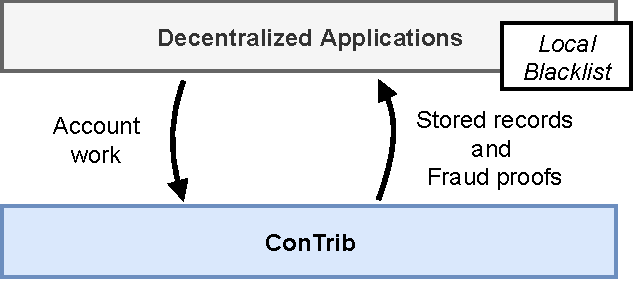
\includegraphics[width=.7\linewidth]{trustchain/assets/contrib_app_interaction}
	\caption{Decentralized applications can use \ModelName{} to account the work performed by peers within tamper-evident \emph{records}. These records are used by connected applications to detect free-riders and fraudsters, which are added to a local blacklist. Applications can then choose to refuse services to the peers on the blacklist.}
	\label{fig:interaction_with_apps}
\end{figure}

\ModelName{} enables connected applications to select which work should be accounted.
Figure~\ref{fig:interaction_with_apps} shows how a decentralized application can leverage \ModelName{} to account work.
By inspecting the records in personal ledgers, an application can gather evidence of free-riding behaviour.
Each application maintains a local blacklist with both free-riders and peers that have committed fraud.
Peers refrain from performing work for peers on the blacklist.
\ModelName{} can be deployed to alleviate fairness concerns in a wide range of decentralized applications, including peer-assisted video distribution, anonymous communication networks, and distributed learning environments.

We implement \ModelName{} and evaluate how different parameters impact the efficiency of fraud detection and the network usage.
We find that fraud can be detected within seconds on average, even in larger networks with 10'000 peers where every peer commits fraud, and under a conservative strategy for record exchange.
We also show that \ModelName{} highly tolerates packet loss.

To show the effectiveness of \ModelName{} in a realistic environment, we employ our accounting mechanism to address free-riding behaviour in \Tribler{}.
\Tribler{} is a decentralized application downloaded by over 1.7 million users~\cite{pouwelse2008tribler}.
We specifically use \ModelName{} to account bandwidth exchanges in \Tribler{}s' Tor-like overlay and use the accounted work to refuse services to free-riders.
Our two-year measurements have resulted in over \TrialRecords{} records, created by more than \TrialUsers{} users.
This large-scale deployment trial is a key milestone in our ongoing research effort to solve the tragedy-of-the-commons within Internet communities~\cite{de2018blockchain}.

The main contribution of this work is four-fold:
\begin{enumerate}
	\item \ModelName{}, a \emph{universal mechanism} that maintains fairness in decentralized application by accounting work (Section~\ref{sec:micro_accounting}).
	\item An efficient \emph{fraud detection mechanism} to detect the illegitimate tampering of created records in \ModelName{} (Section~\ref{sec:detecting_fraud}).
	\item An \emph{implementation} and \emph{evaluation} of \ModelName{} with up to 10'000 peers, demonstrating the scalability of our mechanism and showing that fraud can be detected within seconds on average (Section~\ref{sec:system_architecture} and Section~\ref{sec:implementation_evaluation}).
	\item A \emph{two-year deployment trial} of \ModelName{} in \Tribler{}, involving \TrialUsers{} Internet-recruited volunteers. This trial successfully addresses free-riding behaviour in \Tribler{} (Section~\ref{sec:deployment}).
\end{enumerate}

% We introduce ...

% Collective memory ...

%\section{Introduction}
%Free-riding, the act of selfishly benefiting from the usage of shared resources, is a common issue in both real-world and Internet communities~\cite{rose2003internet,adar2000free}.
%This selfish behaviour frequently prevails in Internet communities.
%This behaviour occurs when access to a shared resource is cheap and there are no individual consequences of overusing the good by community members.
%Structural free-riding on collective resources may result in a \emph{tragedy-of-the-commons}, the situation in shared-resource systems where the resource is depleted and the community around the resource collapses~\cite{hardin2009tragedy}.
%In this work, we address this behaviour by introduce a mechanism for digital shared-resource systems where all resource contributions and consumptions are accounted.
%Free-riding is a prevalent strategy within Internet communities.
%For example, digital media is aggressively competing for user attention, a scarce resource, through the unsolicited presentation of invasive banner ads and clickbait articles~\cite{chen2015misleading}.
%Ongoing Denial-of-Service (DOS) attacks on specific machines is another example of free-riding and shows that some individuals selfishly exploit the ubiquitous access to the Internet~\cite{cerf2013revisiting}.
%This behaviour shows that these attackers have a stronger incentive to undermine the security of shared Internet resources, rather than contributing to it.

%Shared-resource systems on the Internet are vulnerable to free-riding behaviour~\cite{locher2006free}.
%These systems are managing individuals with mutual access to computer resources offered to the community (e.g., bandwidth or CPU capacity).
%For example, downloading in the BitTorrent file-sharing network without contributing (seeding) back after the download has finished goes mostly unpunished and is therefore a common strategy~\cite{locher2006free}.
%Free-riding also occurs in anonymous networks like Tor, where users free-ride on the services offered by relay and exit nodes, without offering community services in return.
%Failure to acknowledge the presence of free-riding behaviour in peer-to-peer networks degrades the systems performance and could eventually result in users permanently leaving the network, as illustrated by the Gnutella software~\cite{adar2000free}.

%To date, the \emph{tragedy-of-the-commons} in Internet communities remains unsolved~\cite{harris2018institutional}.
%This social dilemma occurs where the community around a shared resource, e.g., storage capacity or bandwidth, will eventually collapse due to overexploitation when individual self-interest is at odds with community interests.
%A well-known example is \emph{free-riding} in file-sharing networks, where the act of downloading content without contributing (seeding) back after the download has finished goes mostly unpunished~\cite{locher2006free}.
%Long-term non-cooperative behaviour in shared-resource systems degrades the network performance and eventually leads to a community collapse as illustrated by peer-to-peer applications like  Gnutella~\cite{adar2000free}.

%The Internet has turned into a grim place, where selfish interest of big tech companies supersedes the importance of user-managed communities.
%Email spam is a prominent example of what happens when bandwidth is abused for selfish reasons.
%Over 45\% of email traffic consists of junk messages and an increasing number of ISPs and hosting providers are being forced to use sophisticated techniques in order to try at least to reduce it.
%Likewise, digital media is competing for user attention through the unsolicited presentation of invasive banner ads and clickbait articles.
%Ongoing DDoS attacks on specific machines show that some individuals have a stronger incentive to undermine the security of the Internet, rather than contributing to it.



%Oftentimes, the allocation of shared resources such as bandwidth is prescribed by the output of an algorithm that considers all historical contributions and consumptions of a peer~\cite{tang2004trust}.
%This trust can be based on historical action, or on a believe that the other agent will reciprocate a service later.
%Trade-based incentive mechanisms rely on remuneration for the volunteer resource sharing by agents, either through credits or monetary value.
%This is the approach taken by volunteer computing services, e.g., Boinc, and blockchain-based resource markets, e.g., FileCoin~\cite{benet2018filecoin} and Orchid~\cite{cannellorchid}.

%Providing meaningful incentives to reciprocate after taking some of its resources is imperative to alleviate free-riding behaviour and boost cooperating amongst participants~\cite{ma2004incentive}.
%Some shared-resource systems rely on a \emph{trade-based incentives} where resource consumption is immediately remunerated using a credit or payment system.
%For example, in many volunteer computing projects offered by BOINC users are rewarded for their contributed resources with virtual credits.
%Likewise, shared-resource systems build on blockchain technology leverage cryptocurrency payments to reward communal services~\cite{benet2018filecoin}.

%With \emph{trust-based incentives}, community members are indirectly reciprocated.
%Usually, the amount of provided and consumed resources to and from the community is expressed in a trust score, which can be computed by a reputation mechanism~\cite{meulpolder2009bartercast}.
%These scores are then used to determine a fair allocation of resources, for example, peers with a higher reputation are granted preferential treatment during periods of congestion.
%These trustworthiness scores can be computed by a reputation algorithm.
%To accurately determine the trustworthiness of individuals, shared-resource systems require a public accounting mechanism that records all interactions between users.
%This work focusses on secure accounting of interactions in such systems.

%There have been several proposals to address free-riding behaviour by securely accounting interactions~\cite{guerraoui2010lifting,haeberlen2007peerreview,mokhtar2014acting}.
%We find, however, that existing work is lacking in two directions.
%First, the design of existing solutions usually considers a specific application, e.g., file-sharing or gossip networks.
%This makes it hard, if not impossible, to re-use these solutions across shared-resource systems with differing resource types.
%Second, existing solutions tend to elevate the authority of specific peers in the network, e.g., by having a user act as witness for others.
%This introduces additional system complexities, e.g., incentivize users to not abuse their authority and to follow the protocol.

%As research points out, the interactions in digital shared-resource systems are usually short-lived and concern a small amount of resources~\cite{seuken2014work}.
%For example, the storage protocol FileCoin~\cite{benet2018filecoin} splits data into many small pieces and remunerate peers for the retrieval of individual pieces.
%Similarly, the BitTorrent file-sharing protocol orients around the transport of small data pieces with a variety of peers.
%Repeated, small interactions allows for lower risk-taking since peers can abort an interaction when its counterparty defects, e.g., when a counterparty goes offline during a file exchange.


%This approach aligns well with existing shared-resource systems where interactions are short-lived and concern a small amount of resources~\cite{seuken2014work}.
%For example, blockchain-based storage networks like FileCoin~\cite{benet2018filecoin} split data into small pieces and remunerate peers for the retrieval of pieces.
%Furthermore, micro-accounting allows for low risk-taking since peers can abort an interaction when its counterparty defects, e.g., when a counterparty goes offline during a file exchange.


%In this work, we design, implement, deploy and evaluate a 
%We identify two key advantages of micro-accounting

%So far, there is no lightweight and reusable \emph{micro-accounting} mechanism, specifically designed for recording small interactions in large shared-resource systems.

%Currently, there is no lightweight mechanism for tamper-proof accounting of community interactions, to the best knowledge of the authors.

% Motivate the need for micro-accounting
% 1) it aligns well with existing systems, e.g., file sharing and bandwidth sharing
% 2) it allows for quick punishment and blacklisting of users, with low value-at-risk

%So far, there has been a wide range of research in designing incentive-compatible mechanisms to prevent free-riding in decentralized networks.
%Many of the proposed models and mechanisms require secure accounting of community contributions, for example, if a peer has donated some storage to a specific peer or has uploaded a file to others.

%Most of these efforts are concentrated on reducing free-riding behaviour in file-sharing communities.
%However, free-riding is also prevalent in other communities, such as anonymity networks~\cite{biryukov2015proof}.
%We also observe that most research in this direction take a clean-slate approach for the implementation of their mechanisms.
%This leads to a large range of different implementations.
%Specifically, there is no universal, resource-agnostic infrastructure to quickly evaluate new mechanisms and policies.
%We argue that furthefr research on the management of Internet commons benefits from such an infrastructure.
%Many of these solutions share commonalities in the infrastructure required to deploy these mechanisms.

%\begin{figure}[b]
%	\centering
%	\includegraphics[width=\linewidth]{assets/components}
%	\caption{Our model for trust-based management of shared Internet resources such as bandwidth and storage.}
%	\label{fig:model}
%\end{figure}

%\begin{figure}[t]
%	\centering
%	\includegraphics[width=\linewidth]{assets/trust_cycle}
%	\caption{Our envisioned approach to address free-riding behaviour in large-scale shared-resource systems.}
%	\label{fig:trust_cycle}
%\end{figure}

%We present \ModelName{}, a universal accounting mechanism for the detection of free-riding behaviour in shared-resource systems.
%Our mechanism enables resource accounting where fraud, e.g., illegitimate tempering of micro-records, can be efficiently detected across different shared-resource applications.
%\emph{Micro-records} are the key building block of \ModelName{} and are linked together in a personal ledger.
%A micro-record describes an interaction from the perspective of one of the involved parties.
%Users continuously share micro-records with random users and validate incoming micro-records against known ones.
%Our simple, yet effective technique enables quick detection of fraud, specifically the situation where an adversary has forked its personal ledger.
%We implement \ModelName{} and systematically evaluate its scalability and resistance against malicious users that undermine the accounting mechanism, e.g., by hiding or modifying the micro-records in their personal ledger.
%Our experiments with up to 1'000 users reveal that \ModelName{} that fraud can be detected well within a minute and that the throughput of \ModelName{} scales linearly with the network size.

%To show the effectiveness and matureness of \ModelName{} in a realistic environment, we leverage our mechanism to record bandwidth traffic in \Tribler{}.
%\Tribler{} is our academic peer-to-peer software and downloaded by over 1 million users.
%Specifically, we use \ModelName{} to account bandwidth exchanges in our Tor-like overlay and refuse services to free-riders during periods of congestion.
%Our 36-months measurements has resulted in over 120 million micro-records, created by over \TrialUsers{} users.
%This large-scale deployment trial is a key milestone in our ongoing research to solve the tragedy-of-the-commons in Internet communities.

%The \ModelName{} mechanism is based on two principles.
%First, we decouple the application logic and accounting primitives, unlike related work in the same domain~\cite{osipkov2006robust}.
%This results in a universal accounting mechanism that is reusable across different application domains.
%Second, \ModelName{} is specifically built to deal with the dynamic nature of peer-to-peer networks, where users quickly join or leave.
%Specifically, we avoid network-wide synchronization, group communication or the explicit management of witness sets, while ensuring that fraud will be detected with reasonable probability.

%This work is a cardinal part of our envisioned approach to solve the tragedy-of-the-commons, see Figure~\ref{fig:trust_cycle}.
%In this approach, peers account all resource contribution and consumptions within tamper-proof \emph{micro-records}.
%\ModelName{} records resource contributions and consumptions.
%Our envisioned next step is that every community member periodically runs a reputation algorithm on the collected micro-records which outputs subjective trustworthiness scores.
%These scores guide resource management, the process of determining which users will be granted access to some shared resource.

%Micro-records are organized in personal ledgers and can capture bilateral interactions between individuals by pointing to other micro-records.

%We identify the components and policies that together form an infrastructure for trust-based management of Internet resources.
%Our middleware is flexible, unlike blockchain-based approaches that require full replication and network-wide consensus.
%We build our middleware based on the model visualized in Figure~\ref{fig:model}.
%All community contributions are recorded on a light-weight and tamper-proof distributed ledger and used to compute trust scores by agents.
%These trust scores are then used to allocate resources to others.
%We identify, design and implement the required policies for the management of Internet resources in decentralized communities.

%We believe that the tragedy of the Internet commons can be solved through trust-based mechanisms.
%In this work, we build the required digital infrastructure and tools for sustainable community management on the Internet: accounting mechanisms, reputation algorithms, allocation policies.
%All presented components have been evaluated and tested through field trials with real users, using our academic software named Tribler.
%Tribler is the result of 15 years of engineering effort and has been downloaded by over 1.x million users.

% Possible system attacks:
% Free-riding
% Misreporting
% Collusion
% White-washing

\section{Background and Problem Description}
This work addresses fairness issues in decentralized applications, in particularly free-riding behaviour.
Many decentralized applications integrate a mechanism to reward peers for performing work~\cite{ma2004incentive}.
We first outline two incentive mechanisms that address free-riding by peers, namely trade-based and trust-based incentives~\cite{ruffo2007fairpeers}.

\subsection{Trade-based Incentives}
With trade-based incentives, performed work by peers is remunerated using a credit or payment system.
Peers that use the services of other peers are required to pay for that service.
Remuneration either occurs immediately after the work is performed or when a certain number of payments is outstanding.
The accrued credits can either be converted to real-world money or are merely useful to show the dedication of a particular peer.
BOINC is a well-known volunteer computing project that rewards users with virtual credits for processing scientific workloads~\cite{anderson2019boinc}.

Blockchain technology also relies on financial remuneration to keep the system secure~\cite{easley2019mining}.
Miners, dedicated peers that maintain the blockchain ledger, are usually rewarded for their efforts.
Specifically, users pay a small fee for each transaction and miners then these fees when including their transactions in the blockchain.
Other decentralized applications have adopted cryptocurrencies as a payment system to reward the performed work.
Filecoin is a decentralized system where users pay with a blockchain-based token to have their data stored by peers~\cite{benet2018filecoin}.
Likewise, TorCoin proposes a mechanism where the relay and exit nodes \enquote{mine} a Bitcoin-derived cryptocurrency by relaying Internet traffic~\cite{ghosh2014torpath}.

Even though trade-based incentives are frequently used to incentivize work, remuneration is not an adequate solution for any decentralized applications, for the following three reasons~\cite{hummel2003earning}.
First, they require the integration of a secure payment infrastructure which complicates the system design and potentially enables new forms of attack, such as coin forgery and double-spending.
Using a central authority to keep track of each peer's balance introduces a central component and poses a single-point-of-failure.
Second, remuneration requires peers to determine the price of a digital service, which can be hard to estimate.
Third, remuneration can result in new forms of unfairness where a few affluent peers exclusively enjoy the services of a decentralized application.
This situation could arise when operating peer-to-peer auctions for the allocation of services.

\subsection{Trust-based Incentives}
Applications implementing trust-based incentives indirectly reward community members for their work.
For example, the system can reward dedicated peers with preferential treatment or provide them access to exclusive services.
This approach often requires peers to keep track of the long-term contributions of other peers using accounting infrastructure~\cite{meulpolder2009bartercast}.
The specifications of accounted work can then be used by the application to detect how a particular peer has contributed to the system.
For instance, the accounted work can be used by a reputation algorithm that outputs a ranking of peers~\cite{karakaya2009free}.
If the ranking of a specific peer is below a threshold, the application can decide to refuse to perform work for this peer until its ranking has improved.
We outline related work that uses work accounting and trust-based incentives.
For an overview of (decentralized) reputation mechanisms and trust models, we refer the interested reader to existing work~\cite{hendrikx2015reputation,bellini2020blockchain}.

Perhaps the most popular decentralized application is BitTorrent, a peer-to-peer file exchange protocol~\cite{cohen2003incentives}.
In BitTorrent, each peer has a limited number of slots to allocate to other peers.
The system uses tit-for-tat, a cooperation strategy where a counterparty loses its slot when it stops to reciprocate.
This simple strategy leads to higher network utilization since long-term free-riders will not be allocated slots.
BitTorrent does not persist all contributions and consumptions of other peers, of but tracks the performance of connected peers for each download.

The InterPlanetary File System (IPFS) is a decentralized system for file storage and exchange~\cite{benet2014ipfs}.
IPFS breaks up files into blocks, which are identifiable by a content identifier.
The original IPFS whitepaper describes bitSwap, a set of tools to exchange blocks while addressing free-riding behaviour through block bartering.
It ensures that peers are incentivized to seed blocks by pair-wise tracking of outstanding \enquote{balances}.
Peers that do not sufficiently share blocks will be ignored by others.

Wallach et al. present different mechanisms for the fair sharing of resources in decentralized applications~\cite{wallach2003enforcing}.
These mechanisms ensure that each peer maintains a log with actions and includes random auditing of logs.
The applicability of their work is exclusive to storage-based application and is not reusable for other decentralized applications.
Osipkov et al. describe an accounting mechanism for file-sharing applications~\cite{osipkov2006robust}.
Specifically, each peer maintains a set of witnesses that monitors all transactions of that peer.

LiFTinG and AcTinG are protocols for tracking free-riding behaviour in gossip-based applications~\cite{guerraoui2010lifting,mokhtar2014acting}.
The LiFTinG protocol exploits the message dynamics between peers and verifies that the content received by a peer is further propagated according to the protocol.
The design depends on a statistical approach and cross-checking of logs to detect free-riders but is not reusable for applications beyond gossip.
AcTinG is a gossip-based dissemination protocol that is resistant against colluding rational peers.

Other approaches maintain a distributed ledger that store information in decentralized applications.
Seuken and Parkes introduce a Sybil-resistant accounting mechanism based on transitive trust~\cite{seuken2014sybil}.
PeerReview is an accountability mechanism to record message exchange between peers~\cite{haeberlen2007peerreview}.
Peers store all network messages in a local log.
Dedicated witnesses continuously audit peers and detect whether a peer has deviated from the protocol.
The FullReview protocol extends PeerReview by addressing selfish behaviour with a game-theoretical model~\cite{diarra2014fullreview}.
Otte et al. present TrustChain, a Sybil-resistant reputation mechanism with an accompanying accounting mechanism~\cite{otte2017trustchain}.
The authors apply their mechanism to address free-riding behaviour in a file-sharing network.
We find that peers in TrustChain cannot engage in the recording of multiple interactions simultaneously, significantly limiting the achievable throughput.
Crosby et al. present a data structure for tamper-evident logging~\cite{crosby2009efficient}.
This data structure orients around the efficient logging of unilateral system events on a server.
Peermint is an accounting mechanism designed for market-based management of decentralized applications~\cite{hausheer2005peermint}.

\subsection{Problem Description}
\label{sec:problem_description}
There currently is no \emph{universal} accounting mechanism that can be used to address fairness issues in decentralized applications, to the best of our knowledge.
We address this shortcoming and describe three challenges when designing such a mechanism.

\textbf{Challenge I: Universality.}
The trust-based solutions that we have identified so far are designed for usage within a single application domain and are infeasible to re-use.
We believe that universality is an important property to address fairness concerns in novel decentralized applications.

\textbf{Challenge II: Full Decentralization without Central Authority.}
To keep our system reusable and universal, we avoid \emph{any} decision making by entities with leveraged authorities and central servers.
The lack of a central authority makes our mechanism \emph{fully decentralized} and easier to deploy.
In general, decentralized mechanisms are less vulnerable to large-scale attacks, tend to scale better, and are more resilient to failure.
They also are an excellent architectural fit with existing decentralized applications without central authorities.

\textbf{Challenge III: Fraud Detection.}
Peers have a natural incentive to misrepresent the magnitude of their efforts to inflate their social standing or to hide information unfavourable to their standing~\cite{meulpolder2009bartercast}.
Our accounting mechanism must address the completeness and correctness of the stored information.
We must \emph{detect the manipulation or hiding of accounted information} and punish adversarial peers accordingly.
We consider the accounting of events that have not occurred in the application out of scope.
%Since different applications are likely to have differing visions on how fraud should be managed, we leave this decision to the application.

%For example, overuse in a file-sharing system can result in a temporary, e.g., 24-hour, ban or even result in ostracization from the community.

%\textbf{Requirement III: Scalability.}
%Open shared-resource systems on the Internet can grow to moderate or large sizes.
%For example, applications like BitTorrent and Tor are used by millions of users.
%We require that our solution \emph{scales} when the network size and number of interactions grow.

%Blockchain technology is increasingly being used to manage shared-resource systems.
%FileCoin, for example, is a decentralized system for renting out user-volunteered storage~\cite{benet2018filecoin}.
%Participants in FileCoin record all interactions (data exchanges) within transactions on a distributed ledger, fully maintained by participants.
%Transactions are bundled in blocks, and each block contains the hash of the prior block.
%The modification of a transaction in one block is detected while reaching a distributed consensus.

%Despite a growing ecosystem around the deployment of blockchain-based applications, blockchain technology have fundamental scalability limitations.
%The key issue is that the network is required to continuously establish consensus on the entire transaction set~\cite{vukolic2015quest}.
%This consensus process is carried out by \emph{miners}, volunteers that manage the blockchain.
%The need for consensus significantly limits the achievable throughput, and imposes high storage and bandwidth requirements.
%The throughput of a blockchain secured by Proof-of-Work is usually limited to hundreds transactions per second at best, by far not sufficient to record interactions in large-scale shared-resource systems.
%Furthermore, participants are required to store the full blockchain, which can grow to considerable sizes (e.g., the Bitcoin blockchain currently requires around 290 GB of storage).\footnote{See https://www.blockchain.com/charts/blocks-size}
%We require a lightweight solution, suitable for deployment in large-scale networks.

%Scalability concerns are partially addressed by layer two solutions, e.g., state channels~\cite{mccorry2019pisa}.
%Transactions in layer two solutions are conducted off-chain and users maintain channels to route payment to other users. % users to create transactions 
%Yet, this technology still rely on a \enquote{primary} blockchain for channel management and dispute resolution.


%\textbf{Requirement III: Full decentralization.}
%Many shared-resource systems avert manipulation concerns by introducing a centralized manager that manages all credits or reputation scores of network participants (e.g., as in BOINC).
%However, users now have to trust the manager that it does not modify the credit or trust scores.
%Furthermore, a centralized manager complicates integration with existing systems since it introduces new roles and adds an additional dependency on external actors.
%In practice, dependency on a critical entity introduced a single point-of-failure since downtime of this entity stall all activity.

%As an alternative, one can leverage semi-decentralized solutions where a group of peers are charged with the system management.
%Blockchain is a semi-decentralized system since there is usually a group of peers of which the majority is assumed to be honest.
%Also, the PeerReview accounting mechanism uses witnesses to periodically inspect the correct behaviour of participants in the network~\cite{haeberlen2007peerreview}.

%This work specifically focusses on resource tracking in shared-resource systems.\todo{do something with this}
%There have been proposals to introduce accountability in distributed systems to either detect faulty behaviour or free-riding.

%Even though it is impossible to establish that the interaction embedded in a record has actually occurred, our micro-accounting mechanism should be able to handle record manipulation.

% Problem 1: detect manipulation
% Problem 2: avoid reliance on TTP

%\begin{figure*}[t!]
%	\centering
%	\begin{subfigure}[t]{.33\textwidth}
%		\centering
%		\captionsetup{width=.9\linewidth}
%		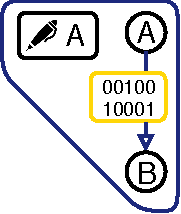
\includegraphics[width=.65\linewidth]{assets/tutorial_1}
%		\caption{To record an interaction between $ A $ and $ B $, $ A $ creates and sign a proposing micro-record (also called a \emph{proposal}).}
%		\label{fig:trustchain_tutorial_1}
%	\end{subfigure}%
%	\begin{subfigure}[t]{.33\textwidth}
%		\centering
%		\captionsetup{width=.89\linewidth}
%		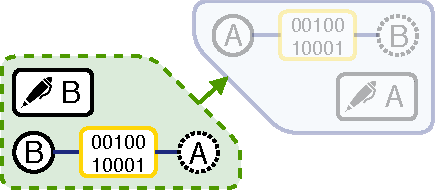
\includegraphics[width=.85\linewidth]{assets/tutorial_2}
%		\caption{Next, $ B $ confirms $ A $'s proposal by creating a confirming micro-record (also called a \emph{confirmation}), that points to it.}
%		\label{fig:trustchain_tutorial_2}
%	\end{subfigure}%
%	\begin{subfigure}[t]{.33\textwidth}
%		\centering
%		\captionsetup{width=.93\linewidth}
%		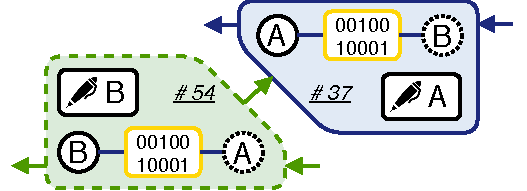
\includegraphics[width=.98\linewidth]{assets/tutorial_3}
%		\caption{To ensure tamper-proofness, we organize micro-records in personal ledgers and reference prior micro-records in a ledger.}
%		\label{fig:trustchain_tutorial_3}
%	\end{subfigure}
%	\caption{Storing an interaction between users $ A $ and $ B $ in \ModelName{} using two micro-records, one proposal and one confirmation. Solid and dotted circular elements indicate the identity of the micro-record creator, respectively, the micro-record counterparty.}
%	\label{fig:trustchain_tutorial}
%\end{figure*}

\section{Accounting Work with \ModelName{}}
\label{sec:micro_accounting}
The design of our universal accounting mechanism, named \emph{\ModelName{}}, is inspired by the tamper-evident properties of blockchain but does not require peers to reach consensus on a coherent history of records.
Instead, \ModelName{} optimistically detects the illegitimate modification of records while keeping the computational overhead and bandwidth requirements low.
Decentralized applications can account the work performed by peers within tamper-evident \emph{records}.
A record describes some work performed by one peer for another peer.
Each peer organizes their records in a \emph{personal ledger}.
Records point to prior records in the same personal ledger and also point to records in the personal ledger of others.
The latter pointer captures an agreement between two peers.
Peers continuously exchange records with other random peers and request records in the personal ledgers of others.
By validating the consistency of incoming records against known ones, a peer can irrefutably prove fraud attempts to other peers.

We further elaborate on the design of \ModelName{}.
We first outline the network and threat model.
We then describe the \ModelName{} data structure and show how \ModelName{} accounts the work in decentralized applications.

\subsection{Network Model}
\label{sec:network_model}
The \ModelName{} mechanism is built on a peer-to-peer network.
We assume an unstructured network structure.
Unstructured networks are relatively straightforward to maintain and are highly resilient against churn.
We assume that the used networking library handles network bootstrapping and peer discovery.
We also assume that the communication channels between peers are unreliable and unordered (e.g., by using the UDP communication model).
The arrival time of messages is not upper-bounded, and outbound messages can fail to arrive at their intended destination.
Each peer has a cryptographic key pair, consisting of a public and private key.
The public key acts as a unique identifier of the peer in the network, whereas the private key is used to sign records and outgoing network messages.
We consider attacks targeted at the network layer, e.g., the Eclipse Attack, outside the scope of this work.

A significant threat in Internet-deployed applications is the Sybil Attack, where an adversary operates multiple identities to subvert the network~\cite{douceur2002sybil}.
The Sybil Attack frequently occurs in open Internet communities, where the cost of creating a new digital identity is often negligible.
Although the \ModelName{} mechanism does not include defences against Sybil identities, we argue that this threat can be mitigated with well-established techniques that complement \ModelName{} in a deployment setting.
A basic defence mechanism is to have peers solve a computational puzzle when they wish to join the network~\cite{li2012sybilcontrol}.
In addition, using a Sybil-resistant reputation mechanism that processes \ModelName{} records can effectively mitigate the effect of Sybil identities on computed trust scores~\cite{delaviz2012sybilres,yu2008sybillimit}.
We also consider self-sovereign identities as a promising solution that can bolster decentralized networks with long-term identities~\cite{stokkink2018deployment}.

We consider misreporting, the accounting of work that has not occurred in the application, beyond the scope of this work.
Misreporting is challenging to address in a generic manner since there is not always a straightforward method to assess if some accounted work is legitimate.
Some protocols use cryptographic techniques to prove the accuracy of performed work, for example, Proof-of-Storage and Proof-of-Bandwidth~\cite{benet2018filecoin,ghosh2014torpath}.
These proofs, however, cannot easily be used across different application domains.

\subsection{Threat Model}
\label{sec:threat_model}
Our threat model orients around malicious peers that attack the integrity of the \ModelName{} data structure.
This attack proceeds through the strategic modification of \ModelName{} records.
For example, a peer can inflate the amount of work it has performed by modifying one of the records in its personal ledger.
We refer to the illegitimate modification of \ModelName{} records as \emph{fraud}.
Even though this definition may seem limited, we argue that this kind of fraud is a fundamental threat to the \ModelName{} data structure.
In particular, our definition of fraud also entails a more advanced form of record manipulations where peers collude to erase a particular interaction from history.
In a reputation system, for example, this would happen when a well-trusted peer temporarily boosts the reputation of another peer by accounting some work and then attempts to hide the existence of this interaction later.
Reverting this interaction requires both counterparties to either override or remove the associated records, which we consider as fraud.
We note that a particular fraud instance in our system involves at most two guilty peers.
As we discussed in Section~\ref{sec:problem_description}, we require that fraud is detected.
We assume that the computing power of adversaries is bounded and that cryptographic primitives are secure.

% Hiding?

%A particular treat is when peers collude in order to record false information, e.g., a bandwidth upload that has not actually occurred within the system.
%It is non-trivial to verify whether the interaction has actually occurred in the system and therefore, we consider this attack outside our scope.
%Addressing this attack likely requires a mechanism that leverages application-specific properties.
%For example, TorPath builds a proof-of-bandwidth that proves that some bandwidth has been transferred through a circuit~\cite{ghosh2014torpath}.
%Creators of fake information should be given a lower trust score by the reputation mechanism, as illustrated in Figure~\ref{fig:trust_cycle}.

%Users store dual-signed agreements of their interactions using \ModelName{} in \emph{micro-records}.

%\begin{table}
%\begin{center}
%	\begin{tabular}{ | p{1cm} | p{6.5cm} | }
%		\hline
%		\textbf{Field} &\textbf{Description} \\
%		\hline
%		$ i $ & The index of the micro-record in the personal ledger of $ a $. \\
%		$ a_{pk} $ & The public key of $ a $. \\
%		$ b_{pk} $ & The public key of $ b $. \\
%		$ t $ & The type of the micro-record. \\
%		$ p $ & The payload of the micro-record. \\ 
%		$ s_{a,i} $ & A digital signature by $ a $ over the micro-record. \\ 
%		$ h_{a,i-1} $ & The hash of the previous micro-record in the personal ledger of $ A $. \\ \hline
%		$ l $ & The index of the referenced proposal. \\ 
%		$ h_{b,l} $ & The hash of a referenced proposal. \\
%		\hline
%	\end{tabular}
%\end{center}
%\caption{The fields in a micro-record created by user $ a $, capturing an interaction with user $ b $. A proposal does not contain the last two fields ($ l $ and $ h_{b,l} $).}
%\label{tab:micro_record}
%\end{table}

\begin{figure}[t]
	\centering
	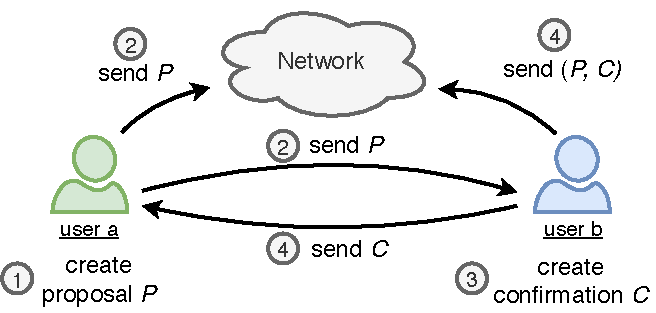
\includegraphics[width=.75\linewidth]{trustchain/assets/interaction}
	\caption{The process of recording work between peers $ a $ and $ b $ within two records: a proposal $ P $ and a confirmation $ C $.}
	\label{fig:interaction}
\end{figure}

\subsection{Recording Interactions}
\label{sec:recording_interactions}
Some work that involves peers $ a $ and $ b $ is recorded using two records: one \emph{proposal} created by $ a $ and one \emph{confirmation} created by $ b $.
W.l.o.g., we assume that the accounted work is performed by peer $ a $ for peer $ b $.
The process of accounting this work is visualized in Figure~\ref{fig:interaction}.
First, $ a $ creates a proposal record, which we refer to as $ P $ (step \circled{1}).
Proposal $ P $, created by peer $ a $, is a tuple with the following four attributes:
\begin{align*}
	P = (\texttt{pubKey}, \texttt{pubKeyOther}, \texttt{payload}, \texttt{sig})
\end{align*}
$ P $ contains the public key of peers $ a $ and $ b $ (\texttt{pubKey} and \texttt{pubKeyOther}, respectively), an application-specific payload (\texttt{payload}), and a digital signature (\texttt{sig}) created by $ a $ of the record in binary form.
The \texttt{payload} attribute is an arbitrary blob of data and is provided by the connected application.
To increase the resilience against manipulation, we extend records with additional fields in the next section.
After peer $ a $ has included all described attributes in the proposal, it persists the record to its database, sends the proposal to $ b $, and disseminated the proposal to $ f $ random peers in the network (step \circled{2}).
We refer to $ f $ as the \emph{fanout} value.

When peer $ b $ receives the proposal $ P $, $ b $ verifies its validity.
It is during this step that fraud is detected.
The validation logic of incoming records is elaborately discussed in Section~\ref{sec:detecting_fraud}.
If the incoming proposal $ P $ is deemed valid, the connected application determines if the payload in $ P $ truthfully describes the performed work.
If $ P $ considered invalid, $ b $ ignores the incoming proposal and takes no further action.
Otherwise, $ b $ creates a confirming record that confirms $ P $ (step \circled{3}).
This confirmation, denoted by $ C $, contains the same attributes as the proposal $ P $ and also includes the hash of $ P $.
Confirmation $ C $, created by peer $ b $ is a tuple with the following five attributes:
\begin{align*}
	C = (\texttt{pubKey}, \texttt{pubKeyOther}, \texttt{payload}, \texttt{proposalHash}, \texttt{sig})
\end{align*}

The value of \texttt{proposalHash} is computed by $ H(P) $, where $ H(\cdot) $ is a secure hash function.
We call the \texttt{proposalHash} attribute in $ C $ the \emph{confirmation pointer}.
After the creation of $ C $, peer $ b $ persists the confirmation to its database, sends it to $ a $, and disseminates both $ P $ and $ C $ to $ f $ random peers (step \circled{4}).
Upon the reception of $ C $, peer $ a $ validates the $ C $ and persists the confirmation if it is valid.
Both parties are now in possession of proposal $ P $ and confirmation $ C $ that together prove an agreement on work between these parties.
The process of accounting work is lightweight since it requires minimal computational power and data exchange. 
Also, peers can engage in the recording of multiple interactions simultaneously.

A potential risk is that $ b $ refuses to confirm $ P $, even though the incoming proposal is valid and contains the correct work details.
This could, for example, occur when confirming $ P $ negatively impacts $ b $'s social standing.
This leaves $ a $ with an unconfirmed proposal, which alone is not sufficient evidence to convince other peers of the performed work by $ a $ for $ b $.
When $ b $ refuses to sign an incoming proposal, $ a $ will add $ b $ to the local blacklist managed by applications, refusing to perform work for $ b $ until $ b $ has confirmed $ P $.
The losses for $ a $ depend on the magnitude of the (unconfirmed) work performed for $ b $.
To minimize these losses, we suggest that decentralized applications record small units of works using \ModelName{}.
For example, a file-sharing application can choose to account unconfirmed work when it reaches a threshold, e.g., 10 MB of traffic exchanged.
Depending on the granularity of accounting, this approach can significantly reduce the impact of peers refusing to acknowledge the contributions of their counterparties.

\subsection{Improving Resilience by Linking Records}
To prevent the modification of created records, we enforce each peer in \ModelName{} to link their records together in a \emph{personal ledger}, incrementally ordered by creation time.
Linking records will also make it harder for malicious peers to hide specific records.
We make the following four modifications to records:

\begin{enumerate}
	\item First, we include a sequence number $ s \in \mathbb{Z} $ in each record that is incremented by one when a new record is added to one's personal ledger.
	The sequence number of the first record in the personal ledger is 1.
	\item Second, each record now includes the hash of the prior record in the personal ledger of the creator.
	This modification makes the \ModelName{} data structure comparable to a hash chain, e.g., as used by blockchain applications.
	The modification of a particular record now changes the hash of subsequent records, a feature that enables us to detect illegitimate changes to stored records (also see Section~\ref{sec:detecting_fraud}).
	The previous hash of the first record in a personal ledger is empty and referred to as $ \bot $.
	\item Third, we extend the confirmation pointer with the sequence number of the proposal record that it confirms.
	\item Forth, we include at most $ b $ additional hashes in each record of distinct, prior records in the same personal ledger.
	We indicate the set with these hashes with $ S $ and call these hashes \emph{back-pointers}.
	As we will further show in Section~\ref{sec:detecting_fraud}, the inclusion of these back-pointers significantly speeds up the detection of fraud.
	The required back-pointers in some record $ R $ are deterministically given by a pseudo-random function $ \sigma $ that takes the public key of the record creator and the sequence number of $ R $ as input.
	$ \sigma $ returns a set with at most $ b $ prior records which hashes should be included in $ R $.
	All peers must use the same version of $ \sigma $, which we achieve by bundling its implementation in the \ModelName{} software.
\end{enumerate}

The above modifications change the attributes of proposal and confirmation records.
We re-define a proposal $ P $, created by peer $ a $ and with counterparty $ b $, as follows:
\begin{align*}
	P = (\texttt{pubKey}, \texttt{pubKeyOther}, \texttt{payload}, \texttt{sig}, \textcolor{ao}{\texttt{seqNum}}, \textcolor{ao}{\texttt{prevHash}}, \textcolor{ao}{\texttt{backPointers}})
\end{align*}
The variables coloured green are new compared to our previous definition of $ P $.
\texttt{seqNum} refers to the sequence number of $ P $, \texttt{prevHash} indicates the hash of the previous record, and \texttt{backPointers} is the set with back-pointers (where $ |S| \leq b $).
We re-define a confirmation $ C $, created by peer $ b $, as follows:
\begin{align*}
	C = (\texttt{pubKey}, \texttt{pubKeyOther}, \texttt{payload}, \textcolor{ao}{\texttt{linkInfo}}, \texttt{sig},
	\textcolor{ao}{\texttt{seqNum}}, \textcolor{ao}{\texttt{prevHash}}, \textcolor{ao}{\texttt{backPointers}})
\end{align*}

We extend confirmations with the same attributes as a proposal but replace the \texttt{proposalHash} attribute with \texttt{linkInfo}.
This is in accordance with our third modification.
\texttt{linkInfo} is now defined as a tuple with the hash and sequence number of the referred proposal record:
\begin{align*}
	C.\texttt{linkInfo} = (\texttt{hash}, \texttt{seqNum})
\end{align*}

Creating records yields the graph structure, as shown in Figure \ref{fig:fullchain}.
Figure \ref{fig:fullchain} shows a part of the \ModelName{} graph with six records, created by three distinct peers ($ a $, $ b $ and $ c $).
Same-coloured records are part of a single personal ledger, and arrows represent hash pointers to other records.
Proposals have a solid border whereas confirmations have a dashed border.
Note how the record in $ a $'s personal ledger with sequence number 55 is unconfirmed.
For presentation clarity, we only show the pointer to the prior record in one's personal ledger and omit additional back-pointers from the figure.

\begin{figure}[t]
	\centering
	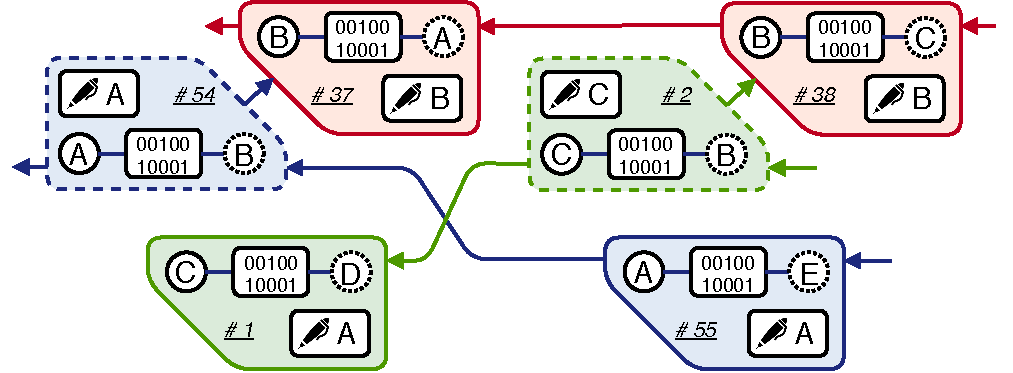
\includegraphics[width=.9\linewidth]{trustchain/assets/fullchain}
	\caption{A part of the \ModelName{} DAG, involving five peers and six records: four proposals (solid borders) and two confirmations (dashed borders). The proposal created by user $ a $ with sequence number 55 is unconfirmed.}
	\label{fig:fullchain}
\end{figure}

\ModelName{} publicly accounts work in interlinked personal ledgers.
Since all performed work is publicly stored and accessible, other users might acquire and analyse \ModelName{} records to reveal potentially sensitive information, e.g., the time at which a particular user is online or the interaction patterns between users.
To reduce this threat, we outline two techniques that applications can use to enhance privacy.
First, applications can account performed and consumed work in \emph{batches}.
For example, an application can record all outstanding contributions and consumptions every hour, therefore hiding granular work statistics.
Second, an application can add some noise to the amount of work being accounted (\emph{fuzzy accounting}).
This technique effectively reduces linkability, e.g., when accounting traffic that is being relayed through multiple hops.
We believe that the combined power of these two techniques provides sufficient privacy guarantees for most decentralized applications.
A more advanced approach, used by the Monero cryptocurrency, leverages ring signatures and zero-knowledge proofs to hide the amounts of work performed~\cite{bunz2018bulletproofs,poelstra2018confidential}.
This approach would, however, require fundamental changes to \ModelName{} and we leave this enhancement for further work.

\section{Detecting Fraud}
\label{sec:detecting_fraud}
We require that \ModelName{} detects illegitimate tampering of the records in a personal ledger.
\ModelName{} is built around fraud \emph{detection} instead of \emph{prevention}.
We argue this is a reasonable assumption for two reasons.
First, decentralized applications often do not require the prevention of fraud~\cite{krishnan2002virtual}.
We argue that fraud prevention is disproportional in the context of work accounting.
Second, preventing fraud is often a resource-intensive process that requires peers to reach a consensus on all created records, e.g., by using classical BFT algorithms or Proof-of-Work~\cite{vukolic2015quest}.
The requirement to reach consensus would severely limit the scalability of \ModelName{}.

Fraud in \ModelName{} occurs when a peer illegitimately modifies one of the records in their personal ledger.
This fraud, for example, happens when an adversary attempts to hide a specific record in the personal ledger by replacing it with another one.
This action would result in pairs of records with the same sequence number and the same creator, but with a different hash.
This violates the integrity of the \ModelName{} data structure.
A key objective of \ModelName{} is to detect such conflicting records quickly.

%According to our threat model, manipulation in \ModelName{} involves an adversary maintaining two different personal ledgers, possibly with a common prefix.
%In related literature, this is often referred to as double-spending or chain forking.

%To incentivize users to participate in the exploration of the \ModelName{} DAG, we propose that collected fraud proofs can be given to resource providers to gain preferential treatment.\todo{elaborate}
%For example, a user $ A $ can modify, reorder or remove micro-records in their personal ledger, and recompute the hash pointers to restore validity.
%However, this basic manipulation can be proven by interaction partners of $ A $ by having them broadcasting the original and manipulated micro-records created by $ A $ with the same sequence number.

%To prove this fraud to others, a user can broadcast the original and manipulated micro-records.

\begin{figure*}[t!]
	\centering
	\begin{subfigure}[t]{.5\textwidth}
		\centering
		\captionsetup{width=.9\linewidth}
		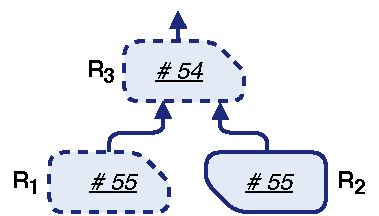
\includegraphics[width=.75\linewidth]{trustchain/assets/fraud_scenario_1}
		\caption{\emph{Scenario I}: Records $ R_1 $ and $ R_2 $ have the same sequence number but a different hash. The pair $ (R_1, R_2) $ is irrefutable proof that peer $ a $ has forked its personal ledger.}
		\label{fig:fraud_scenario_1}
	\end{subfigure}%
	\begin{subfigure}[t]{.5\textwidth}
		\centering
		\captionsetup{width=.89\linewidth}
		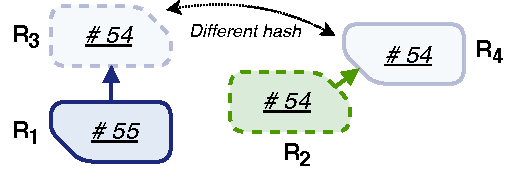
\includegraphics[width=.75\linewidth]{trustchain/assets/fraud_scenario_2}
		\caption{\emph{Scenario II}: Records $ R_3 $ and $ R_4 $ both contain a back-pointer to the record with sequence number 54 but their hashes differ. The pair $ (R_3, R_4) $ is irrefutable proof that peer $ a $ has forked its personal ledger.}
		\label{fig:fraud_scenario_2}\vspace{0.9cm}
	\end{subfigure}
	\begin{subfigure}[t]{.5\textwidth}
		\centering
		\captionsetup{width=.89\linewidth}
		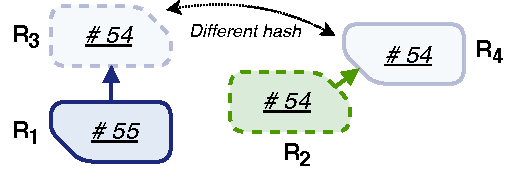
\includegraphics[width=\linewidth]{trustchain/assets/fraud_scenario_3}
		\caption{\emph{Scenario III}: Records $ R_1 $ and $ R_2 $ contain a differing hash of $ a $'s record with sequence number 54. This reveals an inconsistency.}
		\label{fig:fraud_scenario_3}\vspace{0.9cm}
	\end{subfigure}
	\begin{subfigure}[t]{.6\textwidth}
		\centering
		\captionsetup{width=.89\linewidth}
		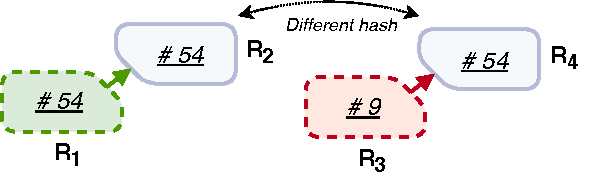
\includegraphics[width=.98\linewidth]{trustchain/assets/fraud_scenario_4}
		\caption{\emph{Scenario IV}: Records $ R_1 $ and $ R_3 $ both confirm $ a $'s record with sequence number 54, but they contain a different hash. This reveals an inconsistency.}
		\label{fig:fraud_scenario_4}
	\end{subfigure}
	\caption{Four scenarios that allows a peer to either expose fraud (forking of a personal ledger), or to detect an inconsistency (without assigning blame). The colour of each record indicates the identity of its creator (blue for $ a $, green for $ b $ and red for $ c $). Solid and dashed records indicate proposals, respectively confirmations. Opaque records are not in possession by the peer.}
	\label{fig:fraud_scenarios}
\end{figure*}

\subsection{Detecting Forks}
\label{sec:detecting_forks}
Fraud in \ModelName{} is detected by sharing newly created records with other peers, and by requesting random records in the personal ledgers of others.
Each peer assesses the consistency of incoming records with the ones in its local database.
This simple approach allows for quick detection of fraud through the collective effort of peers.
In Figure~\ref{fig:fraud_scenarios}, we visualize four identified scenarios in which we can either expose an adversarial peer (scenario I and II) or detect an inconsistency without assigning blame (scenario III and IV).
Each scenario shows the situation from a single peer's perspective and highlights records that a peer has in its local database, or does not have.
Records not in the possession by a peer are faded.
Records with the same colour are created by the same peer.
We discuss each scenario and elaborate on how they either lead to fraud exposure or the detection of an inconsistency.

\begin{itemize}
	\item \textbf{Scenario I}. 
	The first scenario, visualized in Figure~\ref{fig:fraud_scenario_1}, describes a situation where a peer can directly expose a fork in the personal ledger of peer $ a $.
	The personal ledger of peer $ a $ has been forked since records $ R_1 $ and $ R_2 $ have the same sequence number but a different hash.
	As soon as another peer, say $ b $, receives $ R_1 $ while already having $ R_2 $, or receives $ R_2 $ while already having $ R_1 $, the pair $ (R_1, R_2) $ is sufficient evidence to expose the fraud by $ a $.
	The digital signature by $ a $ in the records prove that $ a $ deliberately created both records.
	Note that $ b $ does not need to have $ R_3 $ to detect nor to prove this fraud.
	We call the pair $ (R_1, R_2) $ a \emph{fraud proof}.
	Fraud proofs are by default shared with other peers in the network through a \texttt{FraudProof} message.
	\item \textbf{Scenario II}. The second scenario describes the situation where one can prove fraud by detecting inconsistencies in the included back-pointers of records.
	Figure~\ref{fig:fraud_scenario_2} shows four records created by peer $ a $.
	Records $ R_3 $ and $ R_4 $ contain the hash of the record with sequence number 54 in the back-pointer set; however, these back-pointers describe the same record with a different hash.
	The pair $ (R_3, R_4) $ is irrefutable proof that peer $ a $ has committed fraud and can be used to construct a fraud proof.
	\item \textbf{Scenario III}.
	Figure~\ref{fig:fraud_scenario_3} shows a third scenario where a peer receives proposal $ R_1 $ and already has confirmation $ R_2 $, or receives confirmation $ R_2 $ while already having proposal $ R_1 $.
	The peer does not have records $ R_3 $ and $ R_4 $.
	The hash of record $ R_3 $ in $ R_1 $ differs from the hash in the confirmation pointer in $ R_2 $.
	This situation reveals an inconsistency that is either introduced by peer $ a $ forking its personal ledger at height 54, or by $ b $ having included a wrong hash in $ R_2 $.
	To assign blame, the peer that is validating the incoming record requires either $ R_3 $ or $ R_4 $.
	A peer that encounters this situation sends the pair ($ R_1 $, $ R_2 $) within a \texttt{Inconsistency} message to other random peers, hoping that others will be able to expose the malicious peer.
	\item \textbf{Scenario IV.}
	Figure~\ref{fig:fraud_scenario_4} highlights the fourth scenario where a peer either receives confirmation $ R_1 $ while already having confirmation $ R_3 $, or vice versa.
	Both confirmations point to a record with the same public key and sequence number, but the hash of this record differs.
	This situation either indicates a fork of the personal ledger of $ a $, or it can be the result of an invalid pointer in one of the confirmations.
	Similar to scenario III, the validating peer sends the pair ($ R_1 $, $ R_3 $) within a \texttt{Inconsistency} message to other, random peers.
\end{itemize}

%The other two scenarios, displayed in Figure~\ref{fig:fraud_scenario_2} and Figure~\ref{fig:fraud_scenario_3}, enables the detection of an inconsistency but one cannot assign blame without more context.

%A more advanced manipulation is \emph{forking}, where a user creates two micro-records with the %same sequence number but with different counterparties.
%The goal of this fraud is to hide a specific micro-record from ones personal ledger, e.g., records that indicate some resource consumptions.
%This is similar to the double-spend attack in blockchain ledgers like Bitcoin~\cite{grunspan2018double}.
%Only when a user discovers both conflicting micro-records, this manipulation can be proven.
%In Section~\ref{sec:fraud_detection_experiment} we demonstrate that this fraud can be detected within seconds.
%To prove this fraud, the transaction counterparty reveals both the correct block and the invalid block created by $ A $.

\begin{algorithm}[!t]
	\caption{The validation of the fields in record $ R $.}
	\label{alg:record_data_validation}
	\begin{algorithmic}[1]
		\Procedure{validateFields}{$ R $}  \Comment{Step 1}
		\State $ valid \leftarrow $ true
		\If{$ R.seqNum < 1 $}
		\State $ valid \leftarrow $ false
		\EndIf
		
		\If{\textsc{isConfirmation($ R $)} \textbf{and} $ R.linkInfo.seqNum < 1 $}
		\State $ valid \leftarrow $ false
		\EndIf
		
		\If{\textbf{not} \textsc{publicKeyIsValid}($ R.pubKey $)}
		\State $ valid \leftarrow $ false
		\EndIf
		
		\If{\textbf{not} \textsc{signatureIsValid}($ R.pubKey $, $ R.sig $)}
		\State $ valid \leftarrow $ false
		\EndIf
		
		\If{\textbf{not} \textsc{publicKeyIsValid}($ R.pubKeyOther $)}
		\State $ valid \leftarrow $ false
		\EndIf
		
		\If{$ R.seqNum = 1 $ \textbf{and} $ R.prevHash \not= \bot $}
		\State $ valid \leftarrow $ false
		\EndIf
		
		\State \Return valid
		\EndProcedure
		
	\end{algorithmic}
\end{algorithm}

\subsection{Record Validation Logic}
\label{sec:validation_logic}
Based on the four identified scenarios, we design and describe the validation logic of an incoming record $ R $.
Each peer keeps track of known hashes in a dictionary named \texttt{knownHashes}.
This dictionary is indexed with a tuple, containing the public key and sequence number of a record.
The value of dictionary entries is the hash of the record being queried.
%To simplify the validation logic, proposals and confirmations have the same fields.
%The confirmation pointer is implemented with three fields: \textsc{linkPublicKey}, \textsc{linkSeqNum} and \textsc{linkHash}.
%In a proposal, these fields are set to \textsc{null}.
%Each user maintains a dictionary \textsc{hashes} with known hashes.
The validation logic of incoming records consists of the following five steps:

\begin{algorithm}[t]
	\caption{The consistency validation of hashes in an incoming record against known ones.}
	\label{alg:record_validation_step4}
	\begin{algorithmic}[1]
		
		\Procedure{validateHashes}{R}  \Comment{Step 4}
		\State $ hash \leftarrow knownHashes[(R.pubKey, R.seqNum - 1)] $
		\If{$ hash \not= \bot $ \textbf{and} $ hash \not= R.prevHash $}
		\State \Return false
		\EndIf
		\State
		\For{$ seqNum, hash $ \textbf{in} $ R.backPointers $}
		\State $ known \leftarrow knownHashes[(R.pubKey, seqNum)] $
		\If{$ known \not= \bot $ \textbf{and} $ hash \not= known $}
		\State \Return false
		\EndIf
		\EndFor
		\State \Return true
		\EndProcedure
		
	\end{algorithmic}
\end{algorithm}

\textbf{Step 1.}
We first verify the validity of the fields in incoming record $ R $.
This step is performed by the \textsc{validateFields} procedure, which returns a boolean value indicating whether the fields in the record are valid or not.
A pseudocode description of this procedure is given in Listing~\ref{alg:record_data_validation}.
This step validates the sequence number (line 3), the included public keys (line 7 and 11), and the digital signature (line 9).
If the incoming record is a confirmation, it also verifies that the sequence number in the \texttt{linkInfo} attribute is within a valid range (line 5).
It also checks whether the hash of the prior record is sane when the record is the first in ones personal ledger (line 13).
This step does not compare the validity of $ R $ within the context of other records.
Any error in the included fields of $ R $ is computationally efficient to detect and likely originates from a software bug.

\textbf{Step 2.}
Next, we query the database for a record with the same public key and sequence number as the incoming record $ R $.
If such a record $ R' $ is in the database, we check the equality of $ R $ and $ R' $ by performing a comparison between their included fields.
If $ R \not= R' $, we have detected a fork in the personal ledger of the creator behind $ R $.
We then share the fraud proof $ (R, R') $ with other peers in the network.
During this step, we detect the fraud described by scenario I in Section~\ref{sec:detecting_forks}.

\textbf{Step 3.}
Then, we verify if the hash pointers in the incoming record are consistent with known ones.
This is performed by the \textsc{validateHashes} procedure which pseudocode description is given in Listing~\ref{alg:record_validation_step4}.
This procedure first checks whether the \texttt{prevHash} attribute in $ R $ is consistent with the information in the \texttt{knownHashes} dictionary (line 3).
We then iterate over all included back-pointers and verify the consistency of these hashes with the entries in the \texttt{knownHashes} dictionary (line 6-10).
We can detect the inconsistency described by scenario II during this step.

\textbf{Step 4.}
Next, we compare incoming record $ R $ with a link record, if such a record is available in the database.
When $ R $ is a proposal, we get the corresponding confirmation from the database, and if $ R $ is a confirmation, we get the corresponding proposal.
This step is performed by the the \textsc{validateLink} procedure which pseudocode description is given in Listing~\ref{alg:record_validation_step3}.
We first get the linked record from the database (line 2) and only continue with this validation step if we have this record in the database.
We check whether the public keys included in the proposal and confirmation are consistent (line 9), and verify the consistency of the \texttt{linkInfo} attributes in the confirmation (line 11-14).
We detect the inconsistency described by scenario III during this step (line 15-17).

\textbf{Step 5.}
Finally, we verify the validity of the included payload, which is an application-dependent validation procedure.
As we will further outline in Section~\ref{sec:system_architecture}, decentralized applications using \ModelName{} should implement a \emph{validation} policy that denotes whether the payload of an incoming record is valid in the context of the connected application.

If any of the above steps fail, the record is considered invalid.

\begin{algorithm}[t]
	\caption{The validation of an incoming record against a linked record.}
	\label{alg:record_validation_step3}
	\begin{algorithmic}[1]
		\Procedure{validateLink}{R}  \Comment{Step 3}
		\State $ linked \leftarrow db $.\textsc{getLinked(R)}
		\If{$ linked = \bot $}
		\State \Return true
		\EndIf
		\State
		\State $ proposal \leftarrow linked $ \textbf{if} \textsc{isConfirmation(R)} \textbf{else} $ R $
		\State $ confirmation \leftarrow linked $ \textbf{if} \textsc{isConfirmation($ linked $)} \textbf{else} $ R $
		\State
		\If{$ confirmation.pubKeyOther \not= proposal.pubKey $}
		\State \Return false
		\EndIf
		\If{$ confirmation.linkInfo.seqNum \not= proposal.seqNum $}
		\State \Return false
		\EndIf
		\If{$ confirmation.linkInfo.hash \not= proposal.hash $}
		\State \Return false
		\EndIf
		\State $ linkLinked \leftarrow $ db.\textsc{getLinked(}$ linked $\textsc{)}
		\If{$ linkLinked \not= \bot $ \textbf{or} $ link\_linked \not= R $}
		\State \Return false
		\EndIf
		\State \Return true
		\EndProcedure
	\end{algorithmic}
\end{algorithm}

\subsection{Exchanging Records with Other Peers}
\label{sec:exchanging_records}
The detection of fraud in \ModelName{} depends on peers exchanging records with each other.
A peer is motivated to share collected records with others since they might eventually reveal fraud conducted by one of their former counterparties.
So far, we have not discussed how records are disseminated.
Record dissemination is an essential process that affects the speed at which fraud can be detected.
For example, a slow record exchange strategy is likely to increase fraud detection times compared to more aggressive record dissemination.
We consider both \emph{push-based} and \emph{pull-based} exchange of records, which is explained next.

\textbf{Pull-based Record Exchange.}
Each peer by default requests (pulls) records from other random peers at a fixed rate by sending out \texttt{Request} messages.
Applications can choose to send out \texttt{Request} messages to specific peers to build profile information about that peer, e.g., to detect free-riders.
A \texttt{Request} message contains a list of sequence numbers that the recipient should send back.
When receiving a \texttt{Request} message, the recipient also includes linked proposal or confirmation records in the response.
When a peer $ a $ does not respond with records within a reasonable time, the requesting peer adds $ a $ to the local blacklist.

\textbf{Push-based Record Exchange.}
\ModelName{} also supports push-based record exchange, where the creator of a record disseminates it to $ f $ random other peers (as also discussed in Section~\ref{sec:recording_interactions}).
This push-based exchange allows for quick detection of fraud since the probability of no user receiving two conflicting records goes to zero quickly, even when the network size increases~\cite{osipkov2007combating}.
Even if the malicious peer refrains from broadcasting a conflicting record, the counterparty is very likely to do so, assuming there is no collusion between interacting peers.
Immediate dissemination of created records in the network also increases record availability when the sending peer goes offline.

\begin{figure*}[t]
	\centering
	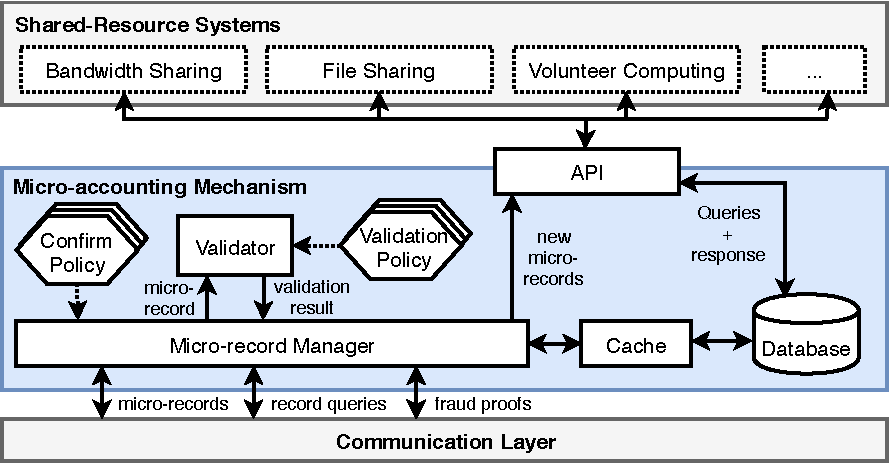
\includegraphics[width=\linewidth]{trustchain/assets/system_architecture}
	\caption{The system architecture of \ModelName{}.}
	\label{fig:system_architecture}
\end{figure*}

\subsection{Limitations}
%In Section~\ref{sec:micro_accounting} and~\ref{sec:detecting_fraud}, we have described how \ModelName{} records are created and how fraud is detected.
Even though our simple algorithm can detect the modification of records, the probabilistic nature of our algorithm can render \ModelName{} unsuitable for deployment in specific application domains.
Since fraud detection is a probabilistic approach, some fraud instances can take relatively long to be uncovered (e.g., several minutes).
We also encountered this behaviour during our experiments (see Section~\ref{sec:implementation_evaluation}).
At the same time, we argue that this is not an insurmountable problem in decentralized applications where performed work holds no or low monetary value.

Since our algorithm is based on fraud \emph{detection}, \ModelName{} is not suitable for applications that require a high level of security, as is the case with decentralized financial applications.
We believe that blockchain technology provides more appropriate security guarantees for such application domains, at the cost of increased resource usage and lower scalability.

Finally, we note that \ModelName{} is mainly built for the lightweight accounting of work in decentralized applications.
In its current state, \ModelName{} cannot capture more complicated operations, e.g., executing arbitrary logic like smart contracts.
However, as demonstrated by recent research advancements, a lightweight accounting mechanism can be an enabling component to devise novel types of decentralized applications with dynamic risk guarantees~\cite{de2020xchange,de2019devid,de2018real}.

% Limitations:
% 1. optimistic detection of fraud -> not everything is detected
% 2. fraud detection is a probablistic process -> detection can take long, depending on several factors

\section{System Architecture}
\label{sec:system_architecture}
We devise a system architecture of our \ModelName{} mechanism, see Figure~\ref{fig:system_architecture}).
The network layer is the lowest layer in our architecture and provides the primitives for decentralised communication and peer discovery.
This layer can be realised using existing frameworks to build peer-to-peer overlay networks, for example, libp2p.\footnote{See \url{https://libp2p.io}}

\textbf{Record Manager.}
The record manager interacts with the network layer to disseminate records and processes incoming ones.
It queues incoming records for validation and persists incoming fraud proofs to the database and connected application.
It also manages the confirmation of incoming and valid proposals targeted at that peer.
Applications using \ModelName{} should provide a \emph{confirmation policy} that predicates whether an incoming proposal should be confirmed.

\textbf{Validator.}
The validator determines the validity of incoming records according to the algorithms described in Section~\ref{sec:validation_logic}.
Connection applications can provide a custom \emph{validation policy}.
If provided, this validation policy is invoked during step 5, when the application-specific payload in a record is validated.
The flexibility to provide custom validation and confirmation policies for incoming records makes \ModelName{} universal and reusable across different application domains.

\textbf{Persistence.}
Records and fraud proofs are persisted in a database.
The \ModelName{} system architecture provides an interface for the queries made to the database and supports different database architectures, e.g., structured or unstructured models.
Our system architecture includes a record \emph{cache}, which is an intermediary component that stores all records in the personal ledger of the operating peer in memory.
This cache allows \ModelName{} to quickly respond to incoming record queries in the personal ledger of the operating peer.
This cache forwards queries to the database for the retrieval and storage of records and fraud proofs.

To contain the growth of the database and to keep the storage overhead manageable, an application can choose to periodically prune the \ModelName{} database when a storage threshold is reached.
In our implementation, by default, we start pruning when at least one million records have been stored.
Applications may increase or decrease this number, depending on the storage capacities of participating peers and the deployment environment.
The default pruning strategy of \ModelName{} continuously removes the record with the lowest database insertion timestamps until the database size has reached its storage threshold again.
The pruning of older records might cause some forks to go undetected since records are removed before a fraud proof can be constructed.
As we will show in Section~\ref{sec:fraud_detection_experiment}, most forks in \ModelName{} are quickly detected, and there should be ample time to detect inconsistencies before relevant records are pruned.

\textbf{Fraud Management.}
When the validation algorithm exposes fraud, or when \ModelName{} receives an incoming fraud proof, the connected applications are notified of the fraud and can punish the misbehaving peer accordingly.
For example, a fraud policy in a bandwidth sharing application could decide to not serve the fraudster for some time.
The decentralised application store the digital identities of fraudsters in a local blacklist.

\textbf{Interactions between \ModelName{} and Applications.}
Decentralised applications interact with \ModelName{} through an API.
This API allows connected applications to query the content of the database.
Furthermore, connected applications can subscribe to incoming records.
The record manager forwards new records to the API, which passes these records to subscribed applications.

\begin{table}[]
	\begin{center}
		\begin{tabular}{l l}
			\hline
			\textbf{Parameter} & \textbf{Default Value}  \\ \hline
			Peers ($ n $) & 1'000 \\
			Workload & 1 proposal per second per peer \\
			Record exchange strategy & \texttt{PULL+RAND+PUSH} \\
			Record fanout ($ f $) & 5 \\
			Record request batch size & 2 \\
			Record request interval & 0.5 seconds \\
			Packet Loss Rate & 0\% \\
			Individual forking probability & 10\% \\
			Back-pointers ($ b $) & 10 \\ \hline
		\end{tabular}
		\caption{The default parameters used during our evaluation.}
		\label{tab:experiment_parameters}
	\end{center}
\end{table}


\section{Implementation and Evaluation}
\label{sec:implementation_evaluation}
Within this section we systematically explore how \ModelName{} behaves when modifying system parameters.
%In the next section we observe how the full implementation of \ModelName{} behaves under real-world conditions and with real Internet users.
We implement \ModelName{} in the Python 3 programming language.
We leverage the network library implemented by our group, and use the UDP protocol for network communication.\footnote{See \url{https://github.com/tribler/py-ipv8}}
Our implementation uses the \texttt{asyncio} framework for asynchronous event handling.
The implementation features both an in-memory storage for experimentation and a persistent (sqlite) database which can be used to persist records over different sessions.
The full implementation of \ModelName{}, including unit tests and documentation, is published on GitHub.\footnote{See \url{https://github.com/tribler/py-ipv8/tree/master/ipv8/attestation/trustchain}}

\subsection{Experiment Setup}
We evaluate the impact of different parameters on the efficiency of fraud detection.
We do so by measuring the time between committing the fraud and its initial detection.
We substitute our networking layer with the SimPy discrete event simulator~\cite{matloff2008introduction}.
Each peer in the \ModelName{} network knows the network address of 100 random other peers, resulting in an unstructured overlay topology.
Table~\ref{tab:experiment_parameters} lists the default parameters during our experiments.
To encourage reproducibility, we have open-sourced the \ModelName{} simulator and all experiment scripts.\footnote{See \url{https://github.com/tribler/trustchain-simulator-pysim}}

\textbf{Workload and Attack Model.}
During our experiments, peers create records with other random peers.
Our default workload has each peer initiate one proposal per second with another random peer.
Note that the rate at which new records are created grows with the network size, which should capture the dynamics of real-world applications (when there are more peers, there is usually more work performed in the application).
We use a uniform transaction load to analyse the characteristics of \ModelName{} under a predictable load.
Even though this transaction load is predictable, it resembles an application where work is periodically accounted.
We experiment with network sizes ranging from 1'000 to 10'000 online peers.
Though some deployed networks have many more peers (e.g., BitTorrent and Tor), our experimental results suggest that \ModelName{} has no issues scaling beyond 10'000 peers.
In Section~\ref{subsec:realistic_workload}, we subject \ModelName{} to a realistic workload, extracted from the interactions in a decentralized file-sharing application.

Each peer forks its personal ledger with a probability of 10\% by removing the last record in its personal ledger and re-using its sequence number to create a new record.
Each peer commits this fraud once.
A peer committing fraud will not broadcast the duplicate record when push-based record exchange is enabled.
In each experiment run, all peers start with an empty personal ledger, and interaction partners always confirm incoming proposals.
A peer that has exposed the fraud of another peer will refuse to confirm the proposals by that peer.
Each experiment run terminates either when all fraud attempts have been discovered or after ten minutes have elapsed.
We are interested in the detection time of fraud instances, which is the time period between committing the fraud and its first detection by a peer in the network.

\textbf{Record Exchange Strategies.}
We consider the following four strategies for exchanging records.
With the \texttt{PULL} strategy, each peer requests two contiguous records at a random height in the personal ledger of another random peer every half a second (the \emph{record request batch size} and \emph{record request interval} parameters in Table~\ref{tab:experiment_parameters}).
Under the \texttt{PULL+RAND} strategy, a peer also returns five random records in their database upon a query.
Including random records in responses enables the detection of fraud of offline peers.
The \texttt{PULL+PUSH} strategy also pushes new records to $ f $ random users upon creation, compared to the \texttt{PULL} strategy.
Finally, we consider the \texttt{PULL+RAND+PUSH} record exchange strategy, which is a combination of the above techniques.

\begin{figure*}[t]
	\centering
	\begin{subfigure}{.8\columnwidth}
		\centering
		
\includegraphics[width=\linewidth]{trustchain/assets/fraud_experiments_legend}
	\end{subfigure}
	\begin{subfigure}{.5\columnwidth}
		\centering
		\captionsetup{width=.9\linewidth}
		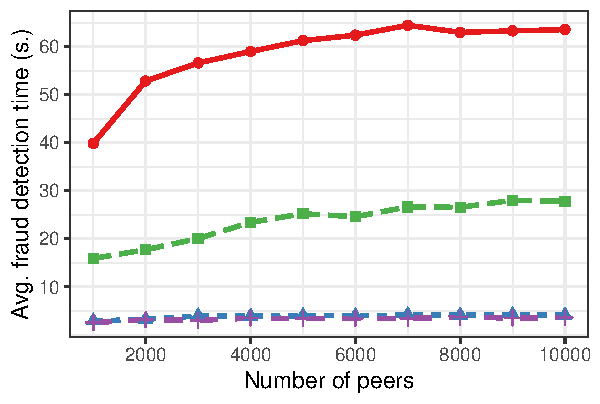
\includegraphics[width=\linewidth]{trustchain/assets/fraud_times_scalability}
		\caption{Average fraud detection times as the number of peers increases.}
		\label{fig:experiment_scalability_detection_times}
	\end{subfigure}%
	\begin{subfigure}{.5\columnwidth}
		\centering
		\captionsetup{width=.9\linewidth}
		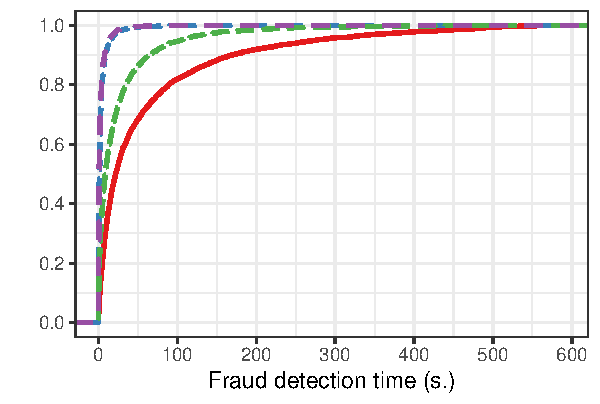
\includegraphics[width=\columnwidth]{trustchain/assets/fraud_times_scalability_5000_ecdf}
		\caption{The Empirical Cumulative Distribution Function (ECDF) for 5'000 peers.}
		\label{fig:experiment_scalability_ecdf_detection_times}
	\end{subfigure}
	\begin{subfigure}{.5\columnwidth}
		\centering
		\captionsetup{width=.9\linewidth}
		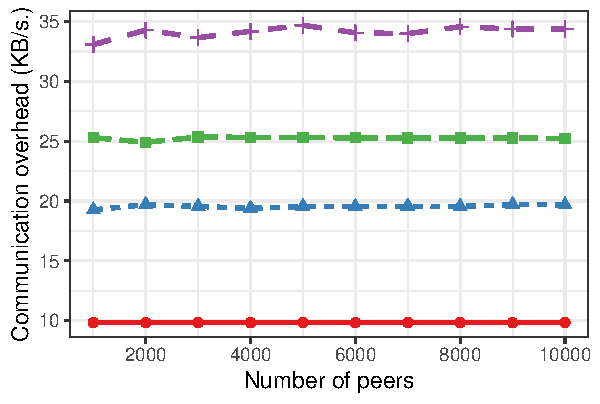
\includegraphics[width=\linewidth]{trustchain/assets/scalability_bandwidth_usage}
		\caption{Average network usage per peer as the number of peers increases.}
		\label{fig:experiment_scalability_bandwidth}
	\end{subfigure}%
	\begin{subfigure}{.5\columnwidth}
		\centering
		\captionsetup{width=.9\linewidth}
		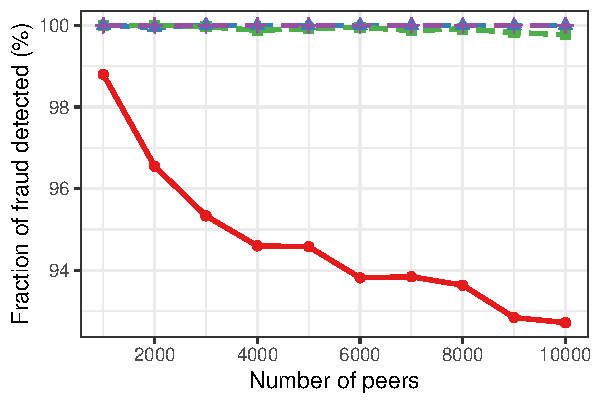
\includegraphics[width=\columnwidth]{trustchain/assets/scalability_num_detected}
		\caption{Fraction of fraud exposed after our experiment ends.}
		\label{fig:experiment_scalability_num_detected}
	\end{subfigure}
	\caption{The results of our scalability experiments, with up to 10'000 peers. We evaluate four record exchange strategies.}
	\label{fig:scalability_experiments}
\end{figure*}

\subsection{Scalability}
\label{sec:fraud_detection_experiment}
Our first experiment quantifies the scalability of \ModelName{} when increasing the number of peers in the network, see Figure~\ref{fig:scalability_experiments}.
Figure~\ref{fig:experiment_scalability_detection_times} shows the effect of increasing the number of peers on the average time until fraud detection, for the four discussed record exchange strategies.
For all record exchange strategies, the average fraud detection time seems to increase when the network size grows.
For $ n = 10'000 $, the \texttt{PULL} strategy shows an average fraud detection time of 63.5 seconds, whereas this number decreases to 3.6 seconds under the \texttt{PULL+RAND+PUSH} strategy.
We notice that the \texttt{PULL+PUSH} and \texttt{PULL+RAND+PUSH} strategies show detection times under five seconds on average.
These low detection times demonstrates that disseminating a record just after its creation is a highly successful strategy.
Including random records in crawl responses also seems to decrease the average fraud detection times.
For $ n = 10'000 $, the average fraud detection time decreases from 63.5 seconds for the \texttt{PULL} strategy to 27.8 seconds for the \texttt{PULL+PUSH} strategy.

In Figure~\ref{fig:experiment_scalability_ecdf_detection_times}, we show the Empirical Cumulative Distribution Function (ECDF) of fraud detection times for $ n = 5'000 $.
We observe that it can take several minutes for some fraud attempts to be discovered, in particular for the \texttt{PULL} and \texttt{PULL+RAND} strategies.
This is not unexpected since fraud detection in \ModelName{} is a highly probabilistic approach.
For the \texttt{PULL} strategy, we can detect 90\% of fraud attempts within 160 seconds and 50\% of the fraud attempts within 30 seconds.
We also observe that the vast majority of fraud is detected within a few seconds when pushing random records after creation.
82.9\% of all fraud attempts are detected within five seconds for the \texttt{PULL+RAND+PUSH} strategy.

Figure~\ref{fig:experiment_scalability_bandwidth} shows the average network usage per-peer as the network size increases, for different record exchange strategies.
The \texttt{PULL} strategy requires less than 10 KB per second of network usage.
Compared to the \texttt{PULL} strategy, the \texttt{PULL+RAND+PUSH} strategy requires more than three times as much bandwidth, around 35 KB per second.
Note how the network usage remains roughly the same for all considered record exchange strategies as we add more peers to the experiment.
Figure~\ref{fig:experiment_scalability_bandwidth} also shows that it is feasible to deploy \ModelName{} in consumer-grade network environments.
System designers can decrease the network usage of \ModelName{} even more by lowering the crawl interval or crawl batch size, at the cost of increased fraud detection times.

Not all fraud has been detected after our experiment has ended.
Figure~\ref{fig:experiment_scalability_num_detected} shows the percentage of fraud attempts that has been detected after the experiment has ended, for an increasing number of peers and different record exchange strategies.
It becomes less likely that fraud is detected during our experiment when increasing the network size under the \texttt{PULL} strategy.
For $ n = 10'000 $, 7.28\% of fraud attempts remain undetected.
These attempts would likely be discovered when prolonging the experiment duration.

%During the experiment, each peer explores others' personal ledgers by continuously querying their latest micro-record, and attempts to detect fraud.
%At the start of each experiment, we selected one peer to perform exactly one double spend attack.
%This peer re-uses the sequence number of the latest micro-record (forking) with 20\% probability.
%We measure the interval between initiation of the fraud and its first detection (upon which the proof can be spread in the network).
%We vary the rate at which users request micro-records from each other.
%We consider request frequencies of 5, 10 and 25 (where 5 means that each user will request a micro-record from five other users every second).
%For each combination of network size and ledger exploration rate, we run the experiment 20 times.

%Figure~\ref{fig:fraud_experiments_fixed_tx} shows the fraud detection times and bandwidth usage while recording 100 interactions per second, for different exchange strategies and network sizes ($ n $).
%Figure~\ref{fig:fraud_experiment_fixed_tx_time} reveals that fraud can be detected within ten seconds under all strategies, even when $ n = 1'000 $.
%The detection times decrease when enabling a push-based exchange strategy (\texttt{PULL+PUSH}), and when sharing random micro-records during a crawl (\texttt{PULL+RAND}).
%Furthermore, the detection times increase roughly linearly when increasing the network size for the \texttt{PULL+PUSH} and \texttt{PULL+RAND+PUSH} strategies.
%In Figure~\ref{fig:fraud_experiment_detect_times_fixed_1000}, we show an ECDF of the detection times for different strategy and with $ n = 1'000 $.
%Note how 50\% of all fraud attempts is detected within ten seconds.
%We notice a significant effect of the push-based exchange strategy on the detection times.
%We explain this effect as follows: pushing created micro-records to random users lead to near-immediate detection of fraud when a user receives two conflicting micro-records.
%Figure~\ref{fig:fraud_experiment_fixed_tx_bw} shows the average bandwidth consumption of each user during our five-minute runs.
%The average bandwidth usage decreases when the network grows which is likely the result of fixing the rate at which new micro-records are created.
%With $ n = 1'000 $, the \texttt{PULL+RAND+PUSH} strategy requires 25KB/s. on average and the \texttt{PULL} strategy only requires 14.5 KB/s.

%Figure~\ref{fig:fraud_experiments_dynamic_tx} shows the detection times and bandwidth usage while scaling the number of recorded interactions with the network size.
%This results in a higher fraud detection times, as hinted by Figure~\ref{fig:fraud_experiment_dynamic_tx_time}.
%Still, fraud attempts are detected within reasonable time: even the \texttt{PULL} strategy enables fraud detection within 22 seconds on average.
%Figure~\ref{fig:fraud_experiment_detect_times_dynamic_1000} shows that the effect of individual strategies on fraud detection times is more pronounced under a dynamic micro-record creation rate.
%Additionally, Figure~\ref{fig:fraud_experiment_dynamic_tx_bw} shows that the average bandwidth usage remains roughly constant when increasing the network size, but slightly drops for $ n > 800 $.
%These experiments show that fraud can be detected efficiently with reasonable bandwidth usage.

%The results are given in Figure \ref{fig:fraud_experiment}.
%The horizontal axis denotes the network size and the vertical axis shows the time interval between performing the forking and its detection.
%The errors bars show one standard deviation of uncertainty.
%Figure \ref{fig:fraud_experiment} shows that faster querying of micro-records increases the speed of fraud detection, at the expense of increased resources usage (bandwidth and CPU utilization).
%We observe that the variation of fraud detection speed is higher when exploring personal ledgers at a lower rate.
%Interesting is that effectiveness of fraud detection shows comparable results when the network size increases.
%Our reasoning for this is as follows: although the specific double spend is more "hidden" in the network, there is also more ongoing effort to detect it.
%This experiment shows that forking of a personal ledger can be detected within mere seconds and 1'000 active peers.

\begin{figure}[t]
	\centering
	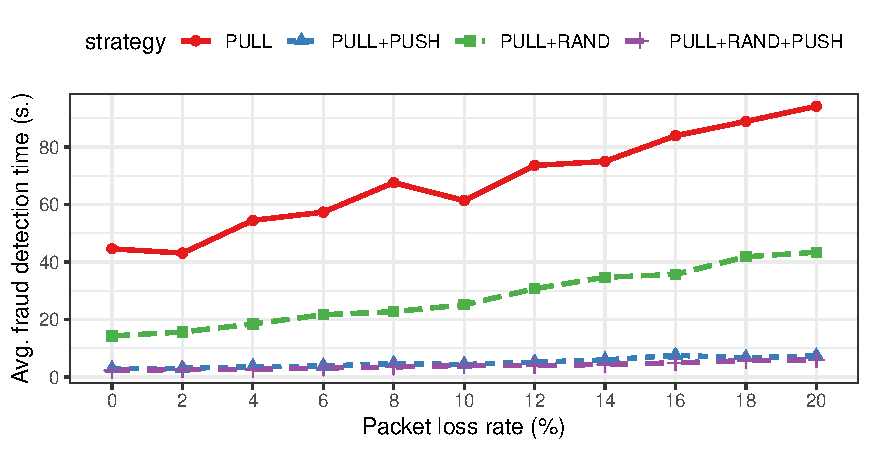
\includegraphics[width=.9\linewidth]{trustchain/assets/fraud_times_send_failure}
	\caption{The effect of packet loss on the average fraud detection times, for different record exchange strategies.}
	\label{fig:fraud_times_link_failures}
\end{figure}

\subsection{Packet Loss}
We reveal the robustness of \ModelName{} by quantifying the effect of packet loss on the efficiency of fraud detection.
To this end, we increase the packet loss rate, up to 20\%, and run our simulations under our four record exchange strategies.
Even though a packet loss rate of 20\% is unlikely for any environment in which \ModelName{} is to be deployed, we want to estimate how robust \ModelName{} is, even in such extreme circumstances.
We expect fraud detection times to increase when network stability is lower since losing packets makes it less likely to detect inconsistencies.

Figure~\ref{fig:fraud_times_link_failures} shows the average fraud detection times when increasing the packet loss rate for our four record exchange strategies.
We observe that fraud detection times increase under the \texttt{PULL} and \texttt{PULL+RAND} strategies, whereas this effect is less for the \texttt{PULL+PUSH} and \texttt{PULL+RAND+PUSH} strategies.
Average fraud detection times, under the \texttt{PULL} strategy, increase from 44.6 seconds with no packet loss to 94.1 seconds when 20\% packet loss.
For the \texttt{PULL+RAND+PUSH} strategy, this same increase is from 2.3 seconds to 6.0 seconds.
We notice that with a packet loss of 20\% and the \texttt{PULL} strategy, 23.8\% of all fraud attempts remains uncovered after the experiment has ended.
This number is just 0.2\% when no packets are lost.
Under the \texttt{PULL+RAND+PUSH} strategy, we see that all fraud attempts are discovered in our experiment, for all evaluated packet loss rates.

\begin{figure}[t]
	\centering
	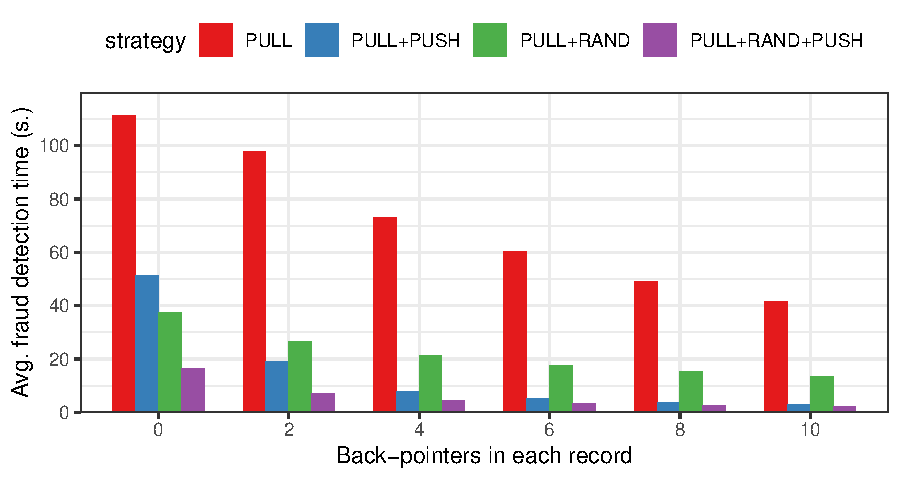
\includegraphics[width=.9\linewidth]{trustchain/assets/fraud_times_back_pointers}
	\caption{The effect of adding more back-pointers to each record on the average fraud detection times, for different record exchange strategies.}
	\label{fig:fraud_times_back_pointers}
\end{figure}

\subsection{Back-Pointers}
We vary the number of back-pointers ($ b $) in each record and analyse the effect on average fraud detection times.
We suspect that adding more back-pointers increases the probability of detecting fraud since individual records now bear more hashes of records in ones personal ledger.
This advantage comes, however, at a cost of additional network usage and computational overhead to analyse the back-pointers.
Each back-pointer adds 32 bytes to the serialized record size.

Figure~\ref{fig:fraud_times_back_pointers} shows the average time until fraud is detected while varying the number of back-pointers and considering different record exchange strategies.
Adding additional back-pointers indeed decreases fraud detection times.
Under the \texttt{PULL} record exchange strategy, it takes 111.2 seconds to detect fraud when no additional back-pointers are included. In comparison, this number decreases to 41.6 seconds when adding up to ten back-pointers to each record (a decrease of 58.4\%).
This decrease is much more for the \texttt{PULL+PUSH} strategy, namely 97\%.
Note that the effect of adding more back-pointers diminishes for $ b > 4 $.
This effect can likely be attributed to the fact that all peers start with an empty personal ledger in our simulations, and that different records with lower sequence numbers in the same personal ledger are more likely to include identical hashes in their back-pointers.
However, we believe that the effect of additional back-pointers becomes more apparent when personal ledgers grow to considerable sizes, since different records are then more likely to include more unique hashes.

\begin{figure}[t]
	\centering
	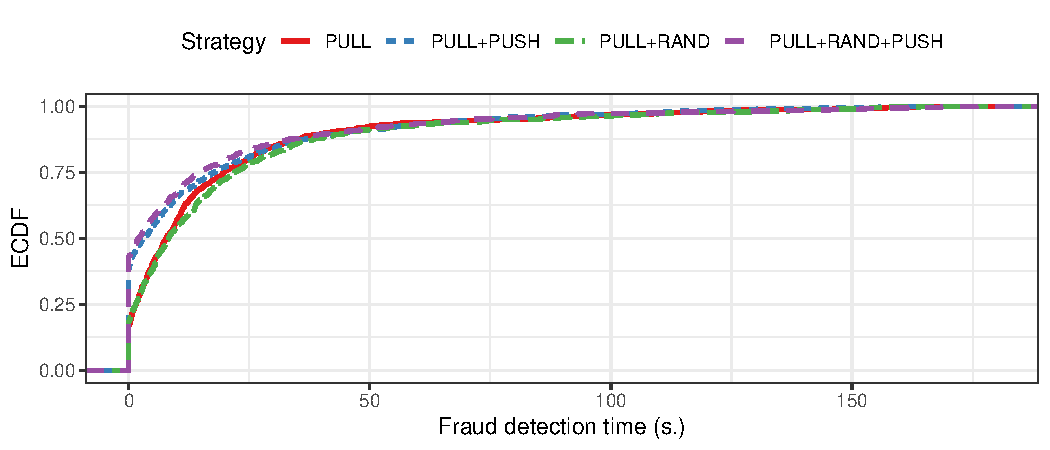
\includegraphics[width=\linewidth]{trustchain/assets/fraud_experiment_realistic_ecdf}
	\caption{Fraud detection times lower than 180 seconds for different record exchange strategies when replaying a day of interactions made by \Tribler{} users.}
	\label{fig:fraud_times_realistic_dataset}
\end{figure}

\subsection{Fraud Detection Times under a Realistic Workload}
\label{subsec:realistic_workload}
Our experiments conducted so far are using a synthetic workload.
We now evaluate the effectiveness of fraud detection in \ModelName{} of our four considered record exchange strategies using a realistic workload.
This workload is derived from deployment data of \ModelName{} in \Tribler{}, our decentralized file-sharing application.
An interaction describes network communication between two peers in a Tor-like overlay.
We provide further details on this dataset in Section~\ref{sec:deployment}.
The following experiment replays interactions made during the busiest 24 hours of our deployment period: November 28, 2020.
On this particular day, a total of 440'130 records have been created, involving 2'027 digital identities.
In the following experiment, we simulate a peer for each digital identity.
In line with our prior experiments, each peer commits fraud with a probability of 10\% when creating a new record.
To match the \ModelName{} settings in our deployed environment (see Section~\ref{sec:deployment}), we increase the record request interval to 10 seconds.

We noticed that all fraud instances have been detected after our experiment ends.
The average fraud detection time for the \texttt{PULL} strategy is just 29.4 seconds whereas this number decreases to 18.5 seconds for the \texttt{PULL+RAND+PUSH} strategy.
2.5\% of all fraud instances take longer than three minutes to detect, with the highest detection time being 1'276 seconds (just over 21 minutes).
Figure~\ref{fig:fraud_times_realistic_dataset} shows the Empirical Cumulative Distribution Function (ECDF) of fraud detection times, for the evaluated strategies.
For presentation clarity, we only show the detection times of fraud instances lower than three minutes.
We observe that over 25\% of all fraud for the \texttt{PULL+PUSH} strategy is detected immediately.
During this experiment, we also see that the network usage per peer is relatively low.
For the \texttt{PULL} strategy, each peer, on average, consumes merely 1.7 MB of hourly network traffic.
This number increases to 5.1 MB under the \texttt{PULL+RAND+PUSH} strategy.

This experiment shows that \ModelName{}, under a realistic workload of \Tribler{} interactions, exhibit relatively low fraud detection times and has low network usage.
As we have also measured during our deployment trial (see Section~\ref{sec:deployment}), the resource overhead of \ModelName{} is minimal.
For \Tribler{}, the fraud detection times shown in Figure~\ref{fig:fraud_times_realistic_dataset} are acceptable.
However, as we have also shown in our other experiments, these detection times can further be improved with more frequent record crawling.

\subsection{Discussion}
In summary, our experiments demonstrate that \ModelName{} exhibits low fraud detection times, scales when the network grows, has reasonable bandwidth overhead, and is robust against packet loss.
We have also demonstrated the effect of the number of back-pointers in each record on the efficiency of fraud detection.
Finally, we have shown that \ModelName{} remains effective at detecting fraud when using a realistic workload.
Even though we have not evaluated the effect of all parameters in Table~\ref{tab:experiment_parameters}, we believe that this set of experiments provides a good starting point for system designers to adopt and configure \ModelName{}.
With our open-source simulator, system designers can quickly analyse the effect of different parameters, guided by a synthetic or realistic workload that resembles the behaviour in their application.

We have demonstrated that there is a trade-off between the average fraud detection times and network usage.
The acceptable network usage differs per applications.
For example, bandwidth is less likely to be a bottleneck when considering a video streaming application compared to an Internet-of-Things environment with low-resource devices.
By reducing the record request intervals, fanout value, and the maximum number of back-pointers, one can reduce the bandwidth footprint of \ModelName{}, at the cost of increased fraud detection times.
Figure~\ref{fig:experiment_scalability_bandwidth} shows that the active record exchange strategy has a notable impact on network usage.
In a dynamic network where the sessions of peers are short-lived, we recommend the \texttt{PULL+RAND} or \texttt{PULL+RAND+PUSH} strategies, where peers share random records in their database with others.
This strategy allows the detection of fraud attempts of offline peers.
We recommend the \texttt{PULL+RAND+PUSH} strategy when fraud must  be detected quickly.
We recommend the \texttt{PULL} strategy when bandwidth is a limiting factor.

\section{Applying \ModelName{} to Address Free-riding at Scale}
\label{sec:deployment}
To show the effectiveness of \ModelName{} with a real-world application, we conduct a large-scale deployment trial of \ModelName{} with \Tribler{}.
\Tribler{} is our decentralized file-sharing application and is downloaded by over 1.8 million users~\cite{pouwelse2008tribler}.
This application features an onion-routing overlay that tunnels BitTorrent traffic through \emph{relay and exit nodes} to provide anonymity.
Unfortunately, the \Tribler{} network suffers from an undersupply of exit nodes, leading to frequent network congestions and overall degradation of download speeds for all users.
We employ \ModelName{} to account the performed work by relay and exit nodes, and the consumed work by downloaders.
We then punish free-riding behaviour by offering users with higher net contributions preferential treatment during periods of congestion.
In the remainder of this section, we elaborate on the integration of \ModelName{} in Tribler, on the collected data, and on the effectiveness of free-riding detection.

\begin{figure}[t]
	\centering
	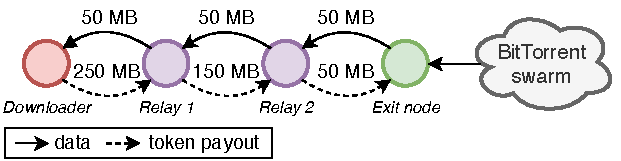
\includegraphics[width=.8\linewidth]{trustchain/assets/payouts}
	\caption{Accounting specifications of an anonymous 50 MB BitTorrent download over a three-hop onion-routing circuit.}
	\label{fig:payouts}
\end{figure}

\subsection{Accounting Bandwidth Transfers}
We enable peers to earn \emph{bandwidth tokens} by providing services as a relay or exit node in the \Tribler{} network.
The mutations in bandwidth token balances of each peer is accounted in \ModelName{} records.
For example, a payout corresponding to a data exchange of a 50 MB file between peers $ a $ and $ b $ deduces 50 MB of $ a $'s balance and increments $ b $'s balance by 50 MB (MB is the unit of this bandwidth token).
Peers can have a negative balance of bandwidth tokens, in which case they have received more traffic than they contributed to the network.

When a peer downloads content using \Tribler{}, the \Tribler{} software establishes a \emph{circuit}, containing exactly one exit node and optionally some relay nodes.
This is comparable to circuits in the Tor protocol.
All traffic is securely routed through relay and exit nodes.
Figure~\ref{fig:payouts} shows how bandwidth tokens are paid out after a peer has downloaded a 50 MB file over a three-hop circuit (with two relay nodes and one exit node).
The downloader accounts a transfer of 250 MB to the first relay using \ModelName{}.
Specifically, the downloader creates a proposal record, containing the pair-wise byte counter with the first relay and the magnitude of the current payout.
In the latest version of \Tribler{}, newly created records are by default disseminated to 20 random peers.
Each peer also requests a random record from another known peer every 10 seconds.
During our deployment period, we have periodically revised the record exchange strategy in response to the network behaviour and growth.

After the downloader has finished the payout to the first relay, the first relay then transfers 150 MB to the next relay, resulting in a net positive token balance of 100 MB for the first relay.
The rationale behind our payout scheme is that we reward relay and exit nodes for performing the cryptographic operations on the forwarded data.
Relays that do not forward the payout to the next hop will be added to the local blacklist by the previous hop, therefore lowering their opportunity to earn bandwidth tokens.
%The payload in \ModelName{} records contains both the token amount transferred and the current token balance of the peer.

Since this use-case involves anonymous downloading, there is an important trade-off between accountability and anonymity.
We plan to address privacy concerns around the accounting of bandwidth transfers by having each peer aggregate and delay payouts.
This privacy-enhancing technique is introduced in the work of Palmieri et al.~\cite{palmieri2015paying}.
Still, work accounting with \ModelName{} does not leak the identity of a downloader to other peers in the network, nor reveals any data being transferred over circuits.
To address the uncontrolled minting of bandwidth tokens by accounting fake work, we are currently looking into the design and deployment of a Sybil-resistant reputation mechanism~\cite{otte2017trustchain}.

\begin{algorithm}[!t]
	\caption{The assignment logic of slots to circuits. \emph{numRand} and \emph{numComp} represent the maximum number of random and competitive slots, respectively.}
	\label{alg:slot_logic}
	\begin{algorithmic}[1]
		\State randomSlots $ \leftarrow [\bot] * $ numRand
		\State competitiveSlots $ \leftarrow [(-\infty, \bot)] * $ numComp
		\State
		
		\Function{onCircuitRequest}{circuit}
		\For{$ i = 0 $ to numRand}
		\If{randomSlots$[i] = \bot $}
		\State randomSlots$[i] \leftarrow $ circuit
		\State \Return
		\EndIf
		\EndFor
		
		\State Query the balance of the initiator of the circuit
		
		\EndFunction
		\State
		
		\Function{onBalance}{circuit, balance}
		\State lowestBalance $ \leftarrow \infty $
		\State lowestIndex $ \leftarrow \infty $
		\For{$ i = 0 $ to numComp}
		\If{competitiveSlots$[i] = (-\infty, \bot) $}
		\State competitiveSlots$[i] \leftarrow $ (circuit, balance)
		\State \Return
		\EndIf
		
		\If{competitiveSlots$[i][0] < $ lowestBalance}
		\State lowestBalance $ \leftarrow $ competitiveSlots$[i][0] $
		\State lowestIndex $ \leftarrow i $
		\EndIf
		\EndFor
		
		\If{balance $ > $ lowestBalance}
		\State \textsc{destroyCircuit}(competitiveSlots$[$lowestIndex$][1] $)
		\State competitiveSlots$[$lowestIndex$] \leftarrow $ (circuit, balance)
		\EndIf
		
		\EndFunction
		
	\end{algorithmic}
\end{algorithm}

\subsection{Circuit Assignment}
We use the bandwidth token balances included in \ModelName{} records to grant preferential treatment to dedicated peers during periods of congestion.
Specifically, we modify the \Tribler{} protocol such that each relay and exit nodes maintain a fixed number of \emph{slots}.
A circuit that includes a relay or exit nodes consumes one slot at their side.
We distinguish between \emph{random} and \emph{competitive} slots.
Random slots are filled on a first-come-first-serve basis whereas the assignment of competitive slot is based on the bandwidth token balance of a circuit initiator.
The intuition behind this approach is to still give peers with lower trust scores an opportunity to earn a (random) slot but at the same time, give preferential treatment to well-behaving peers with competitive slots.
The total number of such slots can be changed, depending on the hardware capabilities of the node operator.

A pseudocode description of the slot assignment logic is given in Listing~\ref{alg:slot_logic}.
When a circuit initiation request arrives, the \texttt{onCircuitRequest} method is invoked and \Tribler{} first determines if there is a random slot available (line 5-9).
If so, we assign the new circuit to the random slot (line 7).
If no random slot is available, \Tribler{} queries the bandwidth token balance of the circuit initiator $ i $ by requesting the records in the personal ledger of $ i $.
When receiving these records, \Tribler{} determines the current bandwidth token balance and checks eligibility for a competitive slot (line 12-23).
If there is an unoccupied competitive slot, \Tribler{} assigns the new circuit to it (line 16).
If all competitive slots are filled, the circuit of the initiator with the lowest amount of bandwidth tokens, say $ p $, is destroyed if the token balance of $ i $ is higher than the token balance of $ p $ (line 22).
This pre-emptive approach frees up the competitive slot for the circuit of $ i $.
As a result, users with a higher token balance have more chance to claim a competitive slot during periods of congestion, compared to free-riders, and experience higher and more stable download speeds.
We consider the analysis of different allocation policies, e.g., using a packet-granular scheduler~\cite{jansen2018kist}, as further work.

%\begin{figure}[t]
%	\centering
%	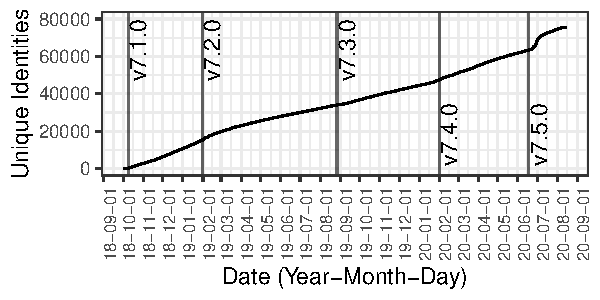
\includegraphics[width=\linewidth]{assets/identities_per_day}
%	\caption{ECDF showing the distribution of bandwidth token balances users and individual rejects events at exit nodes.}
%	\label{fig:identities_per_day}
%\end{figure}

\begin{figure}[!t]
	\centering
	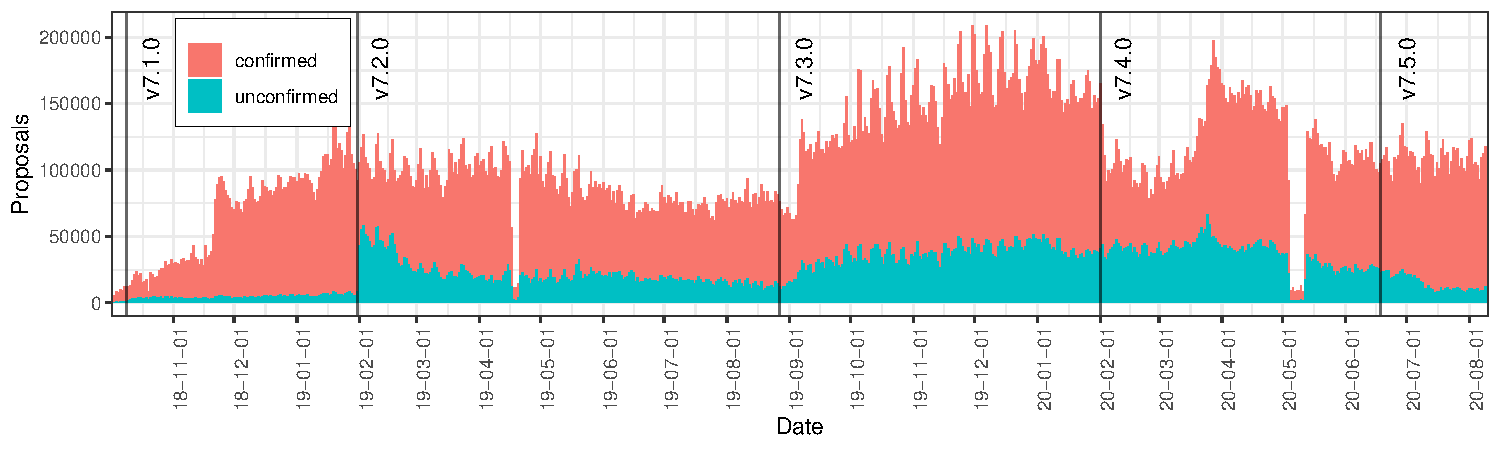
\includegraphics[width=\linewidth]{trustchain/assets/record_creation}
	\caption{Daily creation statistics of proposals, during our two-year deployment trial. We show the amount of confirmed and unconfirmed proposals. We annotate the major releases of \Tribler{}.}
	\label{fig:record_creation}
\end{figure}

\subsection{Data Collection}
We integrate both \ModelName{} and the slot assignment logic in \Tribler{} and release a new version of our software.
We also deploy a crawler that continuously requests \ModelName{} records from random peers in the \Tribler{} network.
This crawler selects a random peer in the \ModelName{} network every two seconds and requests missing records in their personal ledger.
The crawler statistics are published on a public website.\footnote{See \url{http://explorer.tribler.org}}
A deployment period of two years has resulted in more than \TrialRecords{} records, created by over \TrialUsers{} peers.
The crawler stores collected records in a sqlite database that is enhanced with additional indices to speed up insertion and analysis queries.
The file size of the database with all collected records is around 120GB, and we plan on releasing the full data set later.
Our crawler discovered 127'135 proofs of fraud.
We also find that 11.4\% of all collected proposals in the deployed \ModelName{} network is unconfirmed.
This fraction of unconfirmed proposals is either because the proposal counterparty has not created a confirmation, or because our crawler has not picked up the confirmation record.

Deploying a crawler and monitoring the records created by \ModelName{} allows us to detect anomalies caused by software bugs or unexpected user behaviour.
It also provides us with the means to monitor the growth of users within \Tribler{} by tracking the number of unique peers in the \ModelName{} network.
We have also included a creation timestamp in the payload of each record created with \Tribler{}, allowing us to perform a time-based analysis.

Figure~\ref{fig:record_creation} shows the daily number of created proposal records.
We annotate the dates on which we released a major version of \Tribler{}.
Figure~\ref{fig:record_creation} reveals that more users run \Tribler{} during the weekend and create more proposals on a Saturday and a Sunday.
We also observed two large-scale outage of exit nodes, in April 2019 and May 2020, likely due to infrastructure failures.
Despite these outages, users would still perform payouts when downloading directly from other \Tribler{} users without anonymity.

%In \Tribler{}, users earn bandwidth tokens by either operating an exit node, or by relaying traffic.
%By default, users download with one-hop anonymity, meaning that the circuit is directly connected to an available exit node.
%We noticed that only few users increase this setting since adding additional hops to a circuit negatively impacts the achievable download speed.
%There is a delicate trade-off between anonymity and download speed. 
%Therefore, there is an oversupply of relay nodes but the majority of users do not require a relay node for their downloads.
%Eventually, we aim to adjust the default number of hops for a download to two, increasing the opportunities for relay nodes to earn bandwidth tokens.
%We are currently improving the performance of our anonymous download mechanism.

\begin{figure}[t]
	\centering
	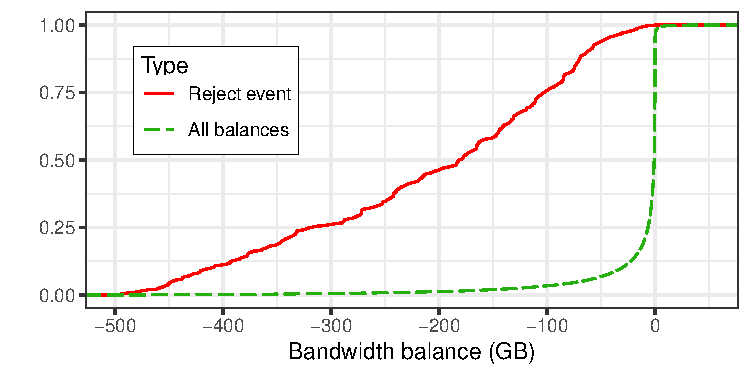
\includegraphics[width=.8\linewidth]{trustchain/assets/exit_node_rejects}
	\caption{Emperical Cumulative Distribution Function (ECDF) of the bandwidth token balances of peers and individual rejects events at exit nodes.}
	\label{fig:exit_node_rejects}
\end{figure}

\subsection{Free-rider Identification and Service Refusal}
To show the effect of \ModelName{} and our slot assignment mechanism on free riders, we deploy 48 exit nodes in the \Tribler{} network, running on the same machine.
Each exit node is configured with a total of 10 random slots and 20 competitive slots, resulting in a total of 1'440 slots.
We determined this number of random and competitive slots based on the hardware capacity of our machine.
We are specifically interested in the situation when a peer is unable to claim a slot, due to their bandwidth token balance being insufficient.
We refer to this situation as a \emph{reject event}.
For each reject event, we log the bandwidth token balance of the rejected peer.
In total, we logged over 1.4 million reject events over three weeks.

Figure~\ref{fig:exit_node_rejects} shows an Empirical Cumulative Distribution Function (ECDF) with the bandwidth token balances of all peers (dotted green line) and the balances associated with rejected circuit requests (solid red line).
For presentation clarity, we filter out all peers and reject events with balances higher than 50GB or lower than -500GB.
Many Tribler users have a negative bandwidth token balance.
The median token balance of all users is -713 MB.
This number suggests that there is not much opportunity to earn bandwidth tokens by contributing to the network.
By default, the Tribler software downloads content over a 1-hop circuit, only involving an exit node.
Changing the default behaviour to use 2-hop downloads could alleviate this issue, at the cost of decreased download speeds.
Figure~\ref{fig:exit_node_rejects} also shows that users with a relatively low (e.g., $ < $ 50 GB) are frequently rejected a slot.
The median token balance associated with reject events is -181.4 GB, demonstrating that our mechanism effectively targets peers with lower bandwidth token balances.
The slots claimed by free-riders will likely go to dedicated peers when the network is congested.
This deployment trial shows that \ModelName{} is effective at detecting and addressing free-riding behaviour in \Tribler{}.
The integration of \ModelName{} has increases network performance and helps to maintain fairness amongst downloading users.

%\begin{figure}[t]
%	\centering
%	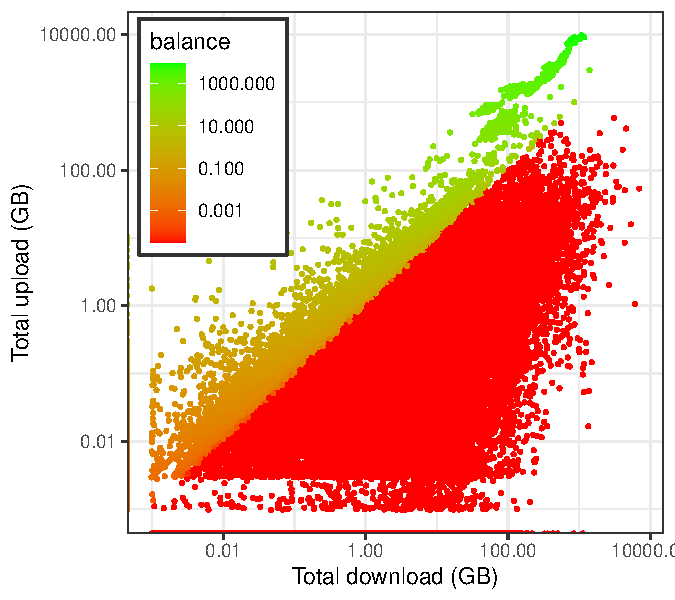
\includegraphics[width=\linewidth]{assets/balances_scatter}
%	\caption{The bandwidth balances of users in Tribler. Users with a balances less than 5GB are marked red.}
%	\label{fig:balances}
%\end{figure}

%\begin{figure}[t]
%	\centering
%	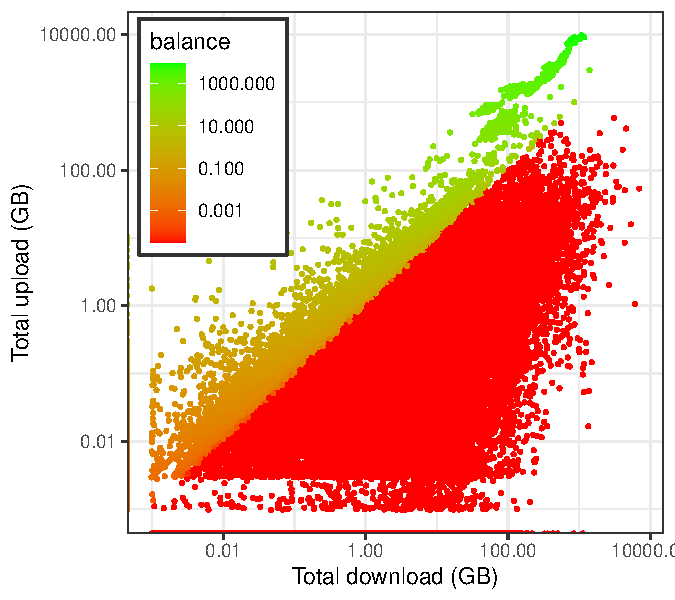
\includegraphics[width=\linewidth]{assets/balances_scatter}
%	\caption{Scatterplot of user balances where each point represents a user in \Tribler{}.}
%	\label{fig:balances_scatter}
%\end{figure}

\section{Conclusion}
We have presented \ModelName{}, a universal accounting mechanism to maintain fairness in decentralized applications by accounting work.
The \ModelName{} data structure uses records to capture the work performed by peers.
Each peer maintains a tamper-evident personal ledger with interlinked records.
Fraud, the illegitimate modification of a record in ones personal ledger, is optimistically detected through the random exchange of records and thorough validation of incoming ones.
We have devised a system architecture of \ModelName{} and implemented it.
Our evaluation has demonstrated that \ModelName{} is capable of detecting fraud within seconds, even when the network grows to 10'000 peers and when scaling the system load.
Through a two-year deployment trial of \ModelName{} in \Tribler{}, involving more than \TrialUsers{} users, we have successfully addressed free-riding behaviour.

We envision and encourage the usage of \ModelName{} beyond work accounting in decentralized applications.
Currently, \ModelName{} is being evaluated in different scenarios that require accountability, including decentralized trading, software developer portfolios, and self-sovereign identity~\cite{de2020xchange,de2019devid,stokkink2018deployment}.
\chapter{MATCH: A Decentralized Middleware for Fair Matchmaking In Peer-to-Peer Markets}
\label{chapter:match}

\emph{
	Order matchmaking is a core enabling element for electronic markets and online economy.
	A common approach to order matchmaking is the deployment of proprietary solutions, controlled by the market operators.
	This approach raises fairness concerns as market operators effectively have the capability to discriminate specific users when matching their orders.
	Blockchain technology has been proposed to enable transparent, open matchmaking solutions without a trusted operator.
	In practice, however, blockchain technology does not provide the required performance, in terms of transaction throughput, for fast order matching across many domains. }
	
\emph{
	In this chapter we present MATCH, a decentralized middleware for fair order matchmaking.
	By decoupling the dissemination of potential matches from the negotiation of trade agreements, MATCH empowers end-users to make their own educated decisions and to engage in direct negotiations with trade partners.
	This approach makes MATCH resilient against matchmakers that pursue selfish interests, a severe issue with centralized matchmaking.
	We implement MATCH and evaluate our middleware using real-world ride-hailing and asset trading workloads.
	It is demonstrated that MATCH maintains high matching quality, even in the presence of malicious matchmakers.
	Further, we show that the bandwidth, memory usage, and order fulfill latency of MATCH is orders of magnitude lower compared to matchmaking on an Ethereum blockchain. }

\newpage

\section{Introduction}
\label{sec:introduction}

The deployment of peer-to-peer markets by companies operating in the sharing economy has been hailed to boost the global economy~\cite{malhotra2014dark}.
Beyond the promises of increased economic welfare, the broader appeal of the sharing economy also lies with the development of new modes for the sharing of unused or underutilized assets, such as cars and houses. %, not unlike other collaborative mechanisms such as crowdfunding and open-source software development. %Reference. Benkler, Y., 2006. The Wealth of Networks: How Social Production Transforms Markets and Freedom, http://benkler.org/Benkler_Wealth_Of_Networks.pdf.
%While there is no single definition for the sharing economy, it can be considered as an umbrella term for novel technology-enabled peer-to-peer markets, enabling new types of interactions on a global scale.
%It has been suggested that the key defining characteristics of sharing economy are markets enabling direct peer-to-peer exchange or rent of under-utilized assets and resources.
%Given the inclusive character of the sharing economy label, the estimates of its size and impact vary. 
Estimations on the impact of the sharing economy suggest an increase in global revenue from \$14 billion in 2014 to \$335 billion by 2025, partially enabled by major platforms such as Uber (ride-hailing) and AirBnb (house-sharing)~\cite{pwcsharingeconomy}. %Reference. PricewaterhouseCoopers. (2015). Consumer Intelligence Series "The Sharing Economy", https://www.pwc.com/us/en/technology/publications/assets/pwc-consumer-intelligence-series-the-sharing-economy.pdf
%Major companies in the sharing economy are Uber (ride-hailing) and AirBnb (house-sharing).

The effect of these platforms on peer-to-peer markets, however, is not unequivocal.
It has been argued that market operators exploit their prominent position and charge high transaction fees for their role as intermediary~\cite{schor2016debating}. %Reference.  (Shapiro 2020) https://onlinelibrary.wiley.com/doi/abs/10.1111/ntwe.12160 
Market operators gain unprecedented power through the control of all the key enabling elements for electronic marketplaces, including settlement, arbitrage, and matchmaking~\cite{oecd2019,pepper2019,azevedo2016}.
%These developments stand in stark contrast with the promises of early peer-to-peer markets, that were envisioned as the enabler for open, fair, and competitive ecosystems~\cite{trastour2002}.
%Currently, however, such markets are mostly enabled by opaque, proprietary matchmaking mechanisms provided by the market operator %Reference. (Shapiro 2020)
The latter element is of particular interest as at the dawn of e-commerce matchmaking solutions were envisioned to create open, fair, and competitive markets on the Internet~\cite{trastour2002}.

Matchmaking in electronic markets can be considered as the process of mediating between supply and demand~\cite{veit2002multi}.
Currently, centralized matchmaking is the approach taken by most commercial market operators~\cite{azevedo2016,oecd2019}.
With centralized matchmaking, market operators deploy proprietary servers that are optimized to efficiently match new buy and sell orders with existing ones within a specific domain.
A key advantage of centralized matchmaking is that the market operator can match incoming orders with the (current) best compatible order since they maintain all market information.
%This approach also enables more simple software integration with other domain-specific services provided by the market operator.

Unfortunately, this also enables market operators to exploit the marketplace through the practices of unfair matchmaking to increase intermediary revenues~\cite{hannak2014}.
Manipulation in the matchmaking process was exposed through analysis of different e-commerce platforms and financial exchanges~\cite{oecd2019,mavroudis2019libra}.
%The scale of this problem is highlighted by the current antitrust investigation into Amazon’s suspected unfair treatment of customers by the European Commission ~\cite{ec2019}.
%It has been also argued that these developments not only introduce unfair competition in e-commerce but can also hurt the effectiveness of emerging peer-to-peer markets. %Reference. (Callo) https://digitalcommons.law.uw.edu/cgi/viewcontent.cgi?article=1046&context=faculty-articles
An emblematic example of this issue is the practices of Uber, implementing price discrimination and phantom matches to manipulate the behaviour of users~\cite{calo2017taking}. %Reference. (Shapiro) 
It has recently been demonstrated through experiments that the matchmaking algorithm of Uber undermines revenues of drivers to the advantages of the platform operator~\cite{bokanyi2019ride}.
As researchers point out, unfair matchmaking is a complex, multilayered issue that can not be mitigated only with algorithmic adjustments~\cite{bokanyi2019ride}.
We suggest that this problem requires a next step towards a different approach to matchmaking in peer-to-peer markets.

It is technologically feasible to have market participants carry out the matchmaking process themselves, without trusted operator.
In particular, blockchain technology provides the means to record and match market orders on a distributed ledger~\cite{subramanian2017decentralized}.
Smart contracts, self-executing programs stored on a blockchain, are capable of executing the matchmaking logic~\cite{luu2016making}.
Even though it seems like an appealing solution to fairness issues, the consensus algorithm managing the blockchain ledger is vulnerable to various attacks against fairness, specifically, \emph{transaction re-ordering} and \emph{front-running}~\cite{eskandari2019,kolluri2018,judmayer2019}.
These attacks effectively allow consensus participants to influence how specific orders are matched.
In addition to these threats, scalability issues inherent to all the blockchain protocols based on a global consensus carry significant limitations on the speed of matchmaking, as we will experimentally show in Section~\ref{sec:experiments_ethereum}~\cite{daian2019}.

%Currently, most of these advancements aim to provide decentralized alternatives to one of the key building blocks of e-commerce: settlement.%Reference. 
%However, decentralized settlement is not sufficient to ensure fair markets~\cite{pesch2019fictions}. %Reference. https://journals.sagepub.com/doi/full/10.1177/0306312719838339
%We suggest that an accompanying approach for decentralized matchmaking is the next logic step towards fair peer-to-peer markets.

The ineffectiveness of matchmaking on a blockchain is also identified by various decentralized exchanges that are operated by a blockchain, also called DEXes~\cite{eskandari2019,warren20170x,idex}.
%At the moment there are little to none solutions providing fair matchmaking in different markets.
In response, these DEXes opt for a federated approach where any participant can host a matchmaking server and can act as a matchmaker.
In practice, most orders in these DEXes are managed by servers that are under the control of the exchange operator and therefore still carry limitations on the achievable level of fairness desirable on such markets.

In summary, there is a dilemma of choice between two desirable properties of matchmaking mechanisms.
%These contradictions effectively create a dilemma of choice 
\emph{Efficiency} of matchmaking achievable through the concentration of orders by a trusted central party, versus provable \emph{fairness} of matchmaking achievable with the transparency of decentralized on-chain matchmaking.
We argue, however, that this dilemma does not present an insurmountable obstacle for the implementation of efficient and fair matchmaking solutions.

\textbf{Contributions.}
We present MATCH, a decentralized middleware for fair matchmaking in peer-to-peer markets.
Our solution is based on the principle of strictly decoupling the matching process from the negotiation of trade agreements.
Our first contribution is the MATCH protocol (Section~\ref{sec:protocol}) where any user can act as a matchmaker for others.
Matchmakers store open orders created by users, match incoming orders with existing ones, and inform order creators about potential matches.
Users then engage in trade negotiation with prospective counterparties.
This approach makes MATCH highly resistant against matchmakers which deviate from a standard matching algorithm. 
The second contribution is the generic MATCH middleware architecture (Section~\ref{sec:architecture}).
MATCH does not rely on the specifications of orders, and is therefore re-usable across different trading domains.
%Order creators disseminate a new order to multiple matchmakers while avoiding network- wide replication of orders.

%We evaluate MATCH using workloads for ride-hailing and asset trading, reconstructed from real world traces.
We devise the first decentralized and fair alternative to the Uber ride-hailing market (Section~\ref{sec:taxi_experiments}), to the best knowledge of the authors.
%We consider ride-hailing (Section~\ref{sec:taxi_experiments}) as a paradigmatic case to demonstrate how fair matchmaking can be achieved without market operator, even when the majority of drivers actively prioritize their own ride services during matchmaking.
Even when 75\% of all drivers prioritize their own ride services during matchmaking, negotiated matches in our market maintain a high quality.
%Unlike centralized matchmaking where orders can be prioritized, hidden, or delayed by a market operator, MATCH provides fair matching for counter-parties who then engage in a peer-to-peer negotiation process with prospective trading partners. 
Furthermore, with a real-world asset trading workload (Section~\ref{sec:asset_trading_experiments}) we show that MATCH is asset-agnostic, enabling the deployment of open and universal matchmaking infrastructures.
%Our experiments demonstrate that MATCH exhibits excellent resistance against selfish matchmakers attempting manipulate matches, while establishing matches with high quality.
Finally, we show that MATCH has bandwidth usage and order fulfil latencies that are several orders of magnitude lower compared to matchmaking on an Ethereum blockchain (Section~\ref{sec:experiments_ethereum}). 

%For decades, the ability to facilitate trade at a global scale has been at the core of many established companies operating on the Internet.
%In 1995, Craigslist already offered an unmoderated mailing list where strangers could meet, negotiate and trade.
%A few years later, eBay enabled traders and merchants to trade physical goods in a trusted manner.
%More recently, leading companies acting within the sharing economy deployed global marketplaces for ride-hailing (Uber), accommodation (Airbnb), freelance labor (TaskRabbit) and many other services~\cite{zervas2017rise}.

%\begin{figure*}[t]
%	\centering
%	\begin{subfigure}[t]{.33\textwidth}
%		\centering
%		\captionsetup{width=.9\linewidth}
%		\includegraphics[width=.9\linewidth]{assets/centralized_matchmaking}
%		\caption{\emph{Centralized matchmaking}: new orders are always sent to a single matchmaker, usually a centralized system (server).}
%		\label{fig:centralized_matchmaking}
%	\end{subfigure}%
%	\begin{subfigure}[t]{.33\textwidth}
%		\centering
%		\captionsetup{width=.9\linewidth}
%		\includegraphics[width=.9\linewidth]{assets/federated_matchmaking}
%		\caption{\emph{Federated matchmaking}: new orders are sent to one of the available matchmakers in the network.}
%		\label{fig:federated_matchmaking}
%	\end{subfigure}%
%	\begin{subfigure}[t]{.33\textwidth}
%		\centering
%		\captionsetup{width=.9\linewidth}
%		\includegraphics[width=.9\linewidth]{assets/decentralized_matchmaking}
%		\caption{\emph{Decentralized matchmaking} (our proposal): new orders are sent to multiple matchmakers and shared between them.}
%		\label{fig:decentralized_matchmaking}
%	\end{subfigure}
%	\caption{Three models for order matching. Traders create offers and requests (colored green and red respectively), which are matched by matchmakers (depicted in blue).}
%	\label{fig:matching_architectures}
%\end{figure*}

% Convince reviewers of the importance of matchmaking


%The main responsibility of many online service providers is to act as \emph{matchmaker} between their users.
%Acting as a trusted intermediary, or \emph{matchmaker}, between users is at the core of many online services providers.
%For example, the key objective of companies acting in the sharing economy, such as AirBnb (house sharing) and Uber (ride hailing), is to bring individuals together that can engage in an exchange of service or goods. %, is to act as trusted middleman for the services provided or requested by individual platform participants.
%Similarly, matching prospective traders with each other is a requirement for e-commerce platform operators such as eBay and Amazon.

%Online commerce platforms are pervasively used in both traditional and emerging markets. However, increasingly becoming critical infrastructure in our society, these platforms also bring systemic risks to everyday consumers~\cite{azevedo2016}\cite{oecd2019}.The full potential of these developments is hard to assess yet, but some key trends are already evident such as an unprecedented concentration of power by a few centralized intermediaries~\cite{pepper2019}.
%The operators of these platforms gain unprecedented power over market flows through the control of all the key enabling elements for marketplaces, including settlement, arbitrage, and matchmaking mechanisms.
%The latter element is of particular interest in this work as at the dawn of e-commerce matchmaking solutions were envisioned as key enabling elements for open and competitive ecosystems of marketplaces~\cite{trastour2002}.

%As a result, however, they increasingly become critical infrastructure in our society~\cite{oecd2019}\cite{azevedo2016} and, with raising influence of a few global players, a systemic risk to everyday consumers.
%However, as they increasingly become critical infrastructure in our society influenced by a few global platforms, it also brings systemic risks to everyday consumers ~\cite{oecd2019}\cite{azevedo2016}.

%Facilitating wide range of interactions between individuals and businesses on the global scale these platform intermediaries start to dominate both traditional and new markets~\cite{oecd2019}.

%The latter element is of particular interest in this work since matchmaking services built on the principles of semantic web became earlier building blocks of scalable e-commerce~\cite{trastour2002}. \todo{not clear how this sentence fits in logically. Why is it of particular interest? Because of semantic web? Because of early e-commerce - then why is it still relevant today?} 
%At the same time development of proprietary matchmaking solutions has significantly outpaced academic research in this area making it difficult to assess wider societal and economic impact
%Effective \emph{matchmaking} between users is an essential enabling component for electronic marketplaces.

%Matchmaking in electronic markets can be considered as the process of mediating between the supply and demand created by users~\cite{veit2002multi}.
%Furthermore, matchmaking can be seen as a universal element for the coordination of economic activity in general, ranging from the matching of asset suppliers to interested buyers, to the assignment of incoming workloads to idle computing resources.

%Currently, \emph{centralized matchmaking} is the approach taken by most commercial market operators~\cite{oecd2019}\cite{azevedo2016}.
%These operators deploy centralized matchmaking servers that are optimized to efficiently match new orders with the existing ones within a specific application domain, which has two main advantages.
%Firstly, the market operator can match incoming orders with the (current) best compatible order, since all orders are stored on their servers.
%Secondly, centralized matchmaking enables more simple software integration with other domain-specific services provided by the same market operator.

%Such opaque, algorithmic matchmaking mechanisms often can be exploited by market-operators to increase their intermediary revenues, through unfair match-making. These practices were identified through different e-comerce platforms [ref]. And the scale of this problem is highlighted by the current antitrust investigation into Amazon's suspected unfair treatment of customers by the European Commission~\cite{ec2019}. It has been also argued that these developments not only introduce unfair competition in e-commerce but can undermine the emerging sharing economy [ref].

%Emblematic of these issue are practices of Uber - operator of ride-hailing platform, implementing price discrimination and phantom matches to manipulate behaviour of its users [ref,ref]. It has been also demonstrated with experimental setups that Uber matchmaking algorithm undermines revenues of participants to the advantages of platforms operator[ref]. As researchers also point out this is a complex, multilayered issues that can not be mitigated only with adjustments in matchmaking algorithms[ref]. We suggest that this problem requires a radical re-thinking the role of trusted third parties as matchmakers. Decentralized matchmaking systems can be a first step towards mitigation of systemic risks stemming from the abuse of privileged intermediary position by market operators.

%Ineffective matchmaking by market operators not only decreases overall market efficiency and customer satisfaction, but also can result in price discrimination and unfair markets~\cite{Wu2015TheM} \cite{mikians2012}.
%For example, in a ride-hailing marketplace like Uber, it is key to match nearby drivers and passengers in a timely and efficient manner.
%For instance, suboptimal matching by ride-hailing marketplaces such as Uber can result in opaque price steering, and greater waiting time both for passengers and drivers~\cite{chen2015} \cite{azevedo2016}. 
%In fact, many of the electronic market operators usually deploy in-house, proprietary matchmaking solutions integrated with price personalization and recommender systems ~\cite{hannak2014}.\footnote{Recommender systems can also be used to enable 'price steering' - changing the order of search results for products and services.}

%Inefficient mediation by such matchmakers decreases the overall platform efficiency and user satisfaction~\cite{Wu2015TheM}.
%For instance, ride-hailing companies assign drivers to waiting passengers based on their geographical separation. % efficiently mediate between passengers, requesting transportation and drivers, willing to provide this service.
%Prolonged sub-optimal matching in this domain increases the waiting time for passengers and results in drivers having to traverse a greater distance to pick up their passengers.
%Equivalently, cloud services providers are tasked to ensure an efficient allocation of their computer resources to customers.
%Failing to do so could violate service-level agreements and result in customer loss and reputational damage.

%Users participate in the market by expressing their intentions in an \emph{order}, which is then submitted to the matchmaking server of the market operator.
%These \emph{centralized matchmaking} servers are optimized to efficiently match new orders with existing ones, within a specific application domain, which has two main advantages.\todo{cite}
%Firstly, the market operator can match incoming orders with the (current) best compatible order, since all orders are stored on their servers.
%Secondly, centralized matchmaking enables more simple software integration with other domain specific services provided by the same market operator.
%it is easier to implement the required software primitives when considering centralized matchmaking, compared to decentralized or distributed matchmaking models.

%For these reasons centralized matchmaking is the approach taken by the most commercial market operators.
%Unfortunately, due to the the proprietary nature of deployed matching algorithms they are specified and controlled by the market operator. 
%Unfortunately, many electronic markets deploy in-house, proprietary matchmaking solutions integrated with price personalization and recommender systems, fully specified and controlled by the market operator~\cite{hannak2014}.\footnote{Recommender systems can also be used to enable \enquote{price steering} by market operator - manipulating the order of search results for products and services in order to nudge users.}
%This raises up a question of contradictions between commercial interests of operators and the objectivity of chosen criteria for matchmaking efficiency~\cite{azevedo2016}.
%Ineffective matchmaking by market operators not only decreases overall market efficiency and customer satisfaction, but also can result in price discrimination and unfair markets~\cite{Wu2015TheM} \cite{mikians2012}.
%Thus, market operators have the capability to modify the matching algorithm so that it gives an (unfair) advantage to specific users \cite{mikians2012}\cite{azevedo2016}.
%Consequentially, the orders of a user might not be matched with the currently best compatible order, resulting in a system that is void of any transparency in the matchmaking process.
%In this model users have to rely on the trustworthiness of the market operator to conduct the matchmaking of their orders in a fair manner and not to engage in price discrimination or other manipulative practices.
%The scale of this problem is highlighted by the current antitrust investigation into Amazon's suspected unfair treatment of customers by the European Commission~\cite{ec2019}.
%The most recent and particularly disturbing illustration is the illegal gouging of prices on the products sold directly by Amazon itself in the heat of COVID-19 epidemic \cite{talmon2020}. 

%Specifically, this server iterates through all existing orders to find matches, based on a matching policy.
%Even though most market operators follow this approach, we identify three deficiencies:
%\begin{itemize}
%	\item \textbf{Unfairness}: 
%Since the matching algorithm is usually not open for inspection by traders, the broker is allowed to match according to their own rules, e.g., to maximize commission fees or to prioritize specific users.

%\item \textbf{Low resistance against large-scale failures}: even though major electronic marketplaces take measure to detect and prevent infrastructure failures, centralized architectures are not resistant against certain events that affect the infrastructure as a whole, e.g., misconfiguration, DNS issues or DDos attacks.
%If the matchmaking infrastructure becomes unavailable, new orders cannot be processed and all market activity stalls.
%\item \textbf{Lack of re-usability}: Due to competitive motivation, the specifications of deployed matchmaking infrastructure and algorithms are often proprietary, and highly domain-specific.
%Therefore, these solutions are not re-usable by other market operators, potentially providing similar services.
%As a result, there exists a large range of non-compatible infrastructure for matchmaking in electronic markets.
%\end{itemize}

%The necessity of a trusted centralized market operator has been challenged by the advancements in decentralized technologies such as blockchain.
%Advancements in decentralized technologies, e.g., blockchain technology, have questioned the role of trusted intermediaries.
%Blockchain technology provides the means to manage a distributed ledger on which users can securely transfer value (e.g., Bitcoin~\cite{nakamoto2019bitcoin}) or deploy decentralized applications (e.g., Ethereum~\cite{wood2014ethereum}) without explicit approval from a trusted third party.
%Decentralized exchanges (DEXes) operating on the basis of blockchain facilitate the trade of digital assets or services without the requirement for a market operator~\cite{subramanian2017decentralized}.
% have resulted in a new type of electronic market: blockchain-based exchanges, or DEXes.
%The problem of efficient matchmaking is re-visited with the deployment of decentralized exchanges based on blockchain technology, also called DEXes.
%These exchanges, also called DEXes, enable traders to securely trade cryptocurrencies and digital assets without a central market operator.
%No trusted third party is needed for the exchange of value, unlike most existing electronic marketplaces.
%In contrast to existing electronic marketplaces, markets powered by blockchain technology, also called DEXes, enable traders to securely exchange digital tokens without a trusted third party.
%The existing research on DEXes addresses the question on \emph{how} to securely exchange value between users, but deems order matchmaking as uninteresting or out of scope~\cite{daian2019}.
%Some DEXes provide one or more matchmaking servers that process market orders~\cite{eskandari2019} ~\cite{idex}\cite{warren20170x}.
%In practice, however, these approaches rely on a few or a single server and therefore still carries limitations on the achievable level of fairness and transparency desirable on such markets.
%Alternatively, the (on-chain) deployment of order matchmaking algorithms on a blockchain addresses the issue of transparency.
%Yet, scalability issues inherent to all the blockchain protocols based on a global consensus carry significant limitations on the speed at which matchmaking can be conducted (also see Section~\ref{sec:experiments_ethereum})~\cite{daian2019}.
%Apart from that, such on-chain implementations based on smart contracts where time and order of transaction execution is critical, demonstrate vulnerability to \emph{transaction re-ordering} and \emph{front-running} attacks ~\cite{eskandari2019}\cite{kolluri2018}\cite{judmayer2019}.
%These contradictions effectively create a dilemma of choice between two desirable properties of matchmaking mechanisms.
%Efficiency of matchmaking achievable through the concentration of orders by a trusted central party, versus provable fairness of matchmaking achievable with the transparency of decentralized on-chain matchmaking.
%We argue, however, that these contradictions do not present an insurmountable obstacle for the implementation of efficient and fair matchmaking solutions. \todo{Georgy (I commented out the contributions)}

%is often performed by a centralized server that collects buy and sell orders, and match them. 
%This centralized approach, however, stands in stark contrast to the decentralized ecosystems that blockchain technology enables.
%Other solutions embed the matchmaking algorithm in the transaction validation process and essentially perform matching on the blockchain (\enquote{on-chain}).
%Unfortunately, this approach is vulnerable to the front-running attack where a specific validator can ultimately decide how specific orders are matched.
%As the number of services for decentralized finance (DeFi) and trade proliferates, there is a growing need for a reliable and re-usable matchmaking mechanism that matches orders in a fair and reliable manner, without centralized control and usable across different domains.
%There currently is no such mechanism available.

%Order matchmaking in various DEXes is a centralized process and performed by a dedicated entity. %/, which is against the decentralized nature of a blockchain ledger.
%Besides aforementioned issues, we argue that centralized matchmaking contradicts the decentralized nature of blockchain ledgers.
%Newer DEX architectures allow for multiple, independent matchmakers that each maintains a list of all current offers and requests~\cite{warren20170x}.
%Traders then submit new orders to one of the available matchmakers.
%New orders created by traders are are matched with others and the exchange of assets then proceeds on the blockchain ledger.

%Within the field of distributed systems, matchmaking is highly related to Publish/Subscribe (pub/sub) architectures\footnote{Some literature in distributed systems refers to an intermediating peer as a \emph{broker}. We use the term matchmaker since we determined it to be more commonly used in related work.}.\todo{rewrite}
%Order brokering is strongly related to Publish/Subscribe (pub/sub) architectures where subscribers indicate their interest in notifications and publishers disseminate new events.
%The main issue is to devise decentralized broker architectures to mediate between publishers and subscribers.
%One might argue that a decentralized pub/sub architecture is sufficient to 
%However, order brokering is a process where the state of individual orders should be updated when successfully matched with other orders, whereas events and notifications in pub/sub systems are static pieces of information.
%Even though there is a substantial body of work on matchmaking in distributed systems, there is no work that researches the properties of decentralized matchmaking in the context of orders.

%Matchmaker is a key concept in Publish/Subscribe (pub/sub) architectures, where one or more brokers deliver events, generated by publishers, to interested subscribers\footnote{Some literature in distributed systems refers to an intermediating peer as a \emph{broker}. We use the term matchmaker since we determined it to be more commonly used in related work.}.
%One might consider an distributed pub/sub architecture where order creators are considered publishers and subscribers are interested in fulfilling specific orders.
%The main issue with this approach is 

%Even though there are many efforts to enable secure value transfer between users without requirement for a trusted broker, there is a lack of understanding \emph{how} these users can connected.
%For this reason, many 

%Matchmaking is defined as the process of mediating supply and demand in markets~\cite{veit2002multi}.

%Notable examples are matching idle agents to incoming jobs or matching suppliers of specific assets to consumers who are interested in buying these assets.

%For example, in a ride-hailing marketplace like Uber, it is key to match nearby drivers and passengers in a timely and efficient manner.
%For instance, prolonged suboptimal matching by ride-hailing marketplaces such as Uber increases the waiting time for passengers and results in drivers having to traverse a greater distance to pick up their customers.


%Traditionally, this is performed by a centralized entity.

%\textbf{Contributions.}
%We present \emph{MATCH}, a decentralized middleware for fair order matchmaking, based on the principle of strictly decoupling the matching process from the negotiation of trade agreements. We evaluate MATCH using two workloads for ride-hailing and asset trading, reconstructed from real world traces. We consider ride-hailing as a paradigmatic case to demonstrate fair decentralized mechanisms for matchmaking. Unlike the centralized matchmaking mechanism where orders can be prioritized, hidden, or delayed by a market operator, MATCH provides fair matching for counter-parties who then engage in a peer-to-peer negotiation process with prospective trading partners.

%Furthermore, with asset trading experiment we show that MATCH does not rely on the specifications of orders, and is therefore re-usable across different trading domains. Our experiments demonstrate that MATCH exhibits excellent resistance against selfish matchmakers attempting manipulate matches, while establishing matches with high quality. Furthermore, we show that MATCH has memory, bandwidth usage, and order fulfill latency that are several orders of magnitude lower compared to matchmaking on an Ethereum blockchain.

%Our main contribution is the MATCH protocol itself where any user can act as a matchmaker for others.
%Matchmakers store open orders created by users, matches incoming orders with existing ones, and inform order creators about potential matches.
%And, since users themselves are ultimately responsible for deciding who they will negotiate with, MATCH exhibits resistance against matchmakers which deviate from an agreed matching algorithm. 
%Order creators disseminate a new order to multiple matchmakers while avoiding network-wide replication of orders. 

%The contribution of this work can be summarized as follows.
%Our first contribution is the MATCH \emph{protocol} where any user can act as a \emph{matchmaker} for others.
%Matchmakers store open orders created by users, matches incoming orders with existing ones, and inform order creators about potential matches.
%Unlike deployed centralized approaches, the role of matchmakers is to \emph{notify} order creators about matching orders and potential counterparties; users then contact these potential counterparties and engage in a peer-to-peer negotiation process.
%Unlike the centralized matchmaking mechanism where orders can be prioritized, hidden, or delayed by a market operator, MATCH provides fair matching for counter-parties who then engage in a peer-to-peer negotiation process with prospective trading partners.
%And, since users themselves are ultimately responsible for deciding who they will negotiate with, MATCH exhibits resistance against matchmakers which deviate from an agreed matching algorithm.
%Order creators disseminate a new order to multiple matchmakers while avoiding network-wide replication of orders.

%The second contribution is the MATCH middleware for fair order matchmaking.
%MATCH does not rely on the specifications of orders, and is therefore re-usable across different trading domains.
%We evaluate MATCH using two workloads for ride-hailing and asset trading, reconstructed from real-world traces.
%Our experiments demonstrate that MATCH exhibits excellent resistance against matchmakers that pursue selfish interests, while establishing matches with high quality.
%Furthermore, we show that MATCH has memory, bandwidth usage, and order fulfill latency that are several orders of magnitude lower compared to matchmaking on an Ethereum blockchain.
%First, in comparison to centralized exchanges, MATCH provides traders with an environment in which that is  \emph{fairness}.
%Second, MATCH is designed around \emph{reliability} and can deal with crash failures of individual brokers.
%Finally, MATCH is \emph{reusable} across different domains that require brokering of homogeneous orders, e.g., the sharing economy, peer-to-peer energy trading and decentralized cryptocurrency exchanges.



%\todo{key insights}

%The main contribution of this work is two-fold.
%Our first contribution is the design of a novel, decentralized order matching protocol.

%Our first contribution is the MATCH middleware, for fair and reliable order brokering in different decentralized environments.
%The second contribution is the MATCH middleware for generic order matching and an accompanying implementation in the Python programming language.

%We identify two problems of existing centralized approaches to matchmaking engines:
%\begin{itemize}
%	\item \textbf{Transparency - } TODO
%	\item \textbf{Unfairness - } TODO
%	\item \textbf{Fault Tolerance - } TODO
%\end{itemize}

%Within the context of distributed systems, there have been efforts to ... \todo{semantic matchmaking}

% The order book 

%Automatically \emph{matching} customers is essential for electronic marketplaces.
%More generally, matchmaking is defined as the process of mediating supply and demand in markets~\cite{veit2002multi}.
%Notable examples are matching idle agents to incoming jobs or matching suppliers of specific assets to consumers who are interested in buying these assets.
%Inefficient matchmaking between participants decreases overall market efficiency and customer satisfaction~\cite{Wu2015TheM}.
%For example, in a ride-hailing marketplace like Uber, it is key to match nearby drivers and passengers in a timely and efficient manner.
%For instance, prolonged suboptimal matching by ride-hailing marketplaces such as Uber increases the waiting time for passengers and results in drivers having to traverse a greater distance to pick up their customers.

%It is common practice for market providers to offer centralized infrastructure that automatically matches new incoming orders with existing ones. %and accepts incoming orders and matches them with other others.
%More specifically, platform participants submit orders to a centralized server.
%This server then attempts to find a match with other orders that are active in the market.
% each company has their own locked-in matching logic.
%All active orders are bundled in an \emph{order book}.
%This data structure keeps track of all market orders that have been submitted by traders.
%New orders, are inserted in the order book and matched against existing entries.
%These servers keep track of the full order book which contains the current list of all active buy and sell orders created by platform participants.
%Centralized matchmaking is deployed by many commercial marketplaces such as Uber, AirBnb and Nasdaq.
%Although this centralized approach to matchmaking is adopted by a vast majority of electronic marketplaces, it leads to a few deficiencies.
%First, centralized order matchmaking architectures tend to be less resistant against infrastructure failures and targeted attacks (e.g., a denial-of-service attack~\cite{mirkovic2004internet}).
%Second, the deployed matching logic is rarely open for inspection by traders and therefore prone to manipulation by market operators.
%For example, Uber has actively manipulated the matching algorithm between drivers and passengers, based on ride pricing~\cite{chen2015peeking}.

%To improve fault tolerance and scalability, the effectiveness of using multiple, independent matchmaking entities has been explored.
%This model, also called \emph{federated matchmaking}, is presented in Figure \ref{fig:federated_matchmaking}.
%The key idea is that each matchmaker takes responsibility for managing a part of the global order book.
%In federated matchmaking architectures, matchmakers often operate highly isolated from each other and do not synchronize orders with each other.
%This isolation potentially leads to missing better matches.

%While numerous electronic marketplaces have deployed (proprietary) matchmaking logic, there is no generic architecture for order matching that is re-usable within different trading domains.
%This results in incompatible applications, all with custom architectural decisions and assumptions regarding workload and environment. % optimized to  under certain assumptions, environments and workloads.
%We address this shortcoming and present MATCH: a middleware for generic order matching.
%Since MATCH does not make any assumptions on the specifications of orders, our middleware i. % and does not make any assumptions on the details of orders being matched.
%This work first outlines two existing models for order matchmaking (Section \ref{sec:background_problem_description}).
%Based on fundamental deficiencies of existing matchmaking approaches, we introduce a new model: \emph{decentralized matchmaking}.
%Next, we present the MATCH protocol, architecture and implementation (Section \ref{sec:protocol}, \ref{sec:architecture} and \ref{sec:implementation}).
%MATCH is designed around the decentralized matchmaking paradigm, yet has full compatibility with existing approaches for order matchmaking. %, while maintaining compatibility with traditional models.
%Finally, we evaluate the performance of MATCH with a ride-hailing and asset trading workload, reconstructed from real-world datasets (Section \ref{sec:experiments}). %, and then design a novel architecture and protocol for decentralized matching of orders.
%This results in an architecture and protocol with high fault tolerance and scalability.

%A major issue is that the matching of two orders by \enquote{consumes} these resources and subsequently should be removed from the order books maintained by brokers.

%In this work, we address the challenging task of devising a network where individual order brokers maintain a decentralized order book.
%These brokers, however, might have adversarial intentions and actively attempt to influence the matchmaking protocol to their own benefits.
%We argue that the availability of such an order book 
%To the best of our knowledge, we are the first to explore order brokering from the context of decentralized markets.

%\newpage

\begin{figure}[t]
	\centering
	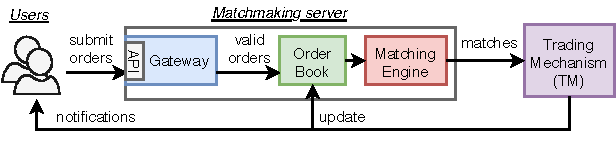
\includegraphics[width=\linewidth]{match/assets/central_exchange_architecture}
	\caption{A generic model for centralized matchmaking in peer-to-peer markets, using a single matchmaking server.}
	\label{fig:central_exchange_architecture}
\end{figure}

\section{Towards Decentralized Matchmaking}
\label{sec:centralized_order_matchmaking}
In our approach, users in a peer-to-peer market conduct the matchmaking process themselves.
To elaborate on the components used in our solution, we first devise a generic, centralized model for matchmaking.
We then identify technical concerns that arise when decentralizing this model.

\subsection{Centralized Matchmaking}
We devise a generic model for centralized matchmaking in peer-to-peer markets, see Figure~\ref{fig:central_exchange_architecture}.
This model is the starting point for our fair matchmaking solution and is inspired by existing architectures that have been widely used by financial markets~\cite{mavroudis2019libra,veit2003matchmaking}.
Users create \emph{orders}, which they then submit to the matchmaking server.
An order specifies interest to buy or sell assets, resources, or services (orders are further discussed in Section~\ref{sec:order_creation}).
Many markets deploy one or more gateways that filter out invalid orders and mitigate targeted attacks on the matchmaking server, such as a DDoS attack~\cite{mavroudis2019libra}.
Valid orders are inserted in the \emph{order book}, a local data structure that bundles all open and valid orders.

Upon the insertion of a new order in the order book, it is forwarded to the \emph{matching engine}.
This component searches for existing orders in the order book that match with the newly submitted order.
In particular, an incoming order should be matched with the current best compatible order(s).
Whether two orders match is predicated by a \emph{matching policy}.
For example, the price-time strategy is a predominant matching policy in financial markets where orders are first matched based on their price and then on their creation time (prioritizing older orders)~\cite{mavroudis2019libra}.
The matching engine can establish multiple matches for a single order, e.g., a buy order for a large number of assets can be matched with multiple (smaller) sell orders.
Established matches should be \enquote{executed}, which is an application-dependent operation.
In a financial exchange, for example, the specified assets in the matched orders should be exchanged between the order creators.
In a ride-hailing market, however, the driver and passenger should be put in contact with each other.
We model the component that executes established matches as the \emph{trading mechanism} (TM), which we consider external to the model in Figure~\ref{fig:central_exchange_architecture}.
After established matches have been executed by the TM, the affected orders in the order book are updated (or removed if they are completed), and the order creators are notified of the match execution.
%Upon receiving a notification from the trading mechanism, the order creator internally updates the state of their affected order.
%We assume that the TM executes matches in a first-come-first-serve manner.
%After a match has been executed, the matched orders in the order book are updated (or removed if the order is completed), and the order creators are notified about this event.
%This unit \enquote{executes} the established matches and ensures that the creators behind these orders trade the services as specified.
%The matching engine forwards established matches to the MPU, updates the matched orders in the order book accordingly, and notifies the user(s) behind the matched orders of the event. % The current state of the order book is updated and matched orders that are completed are removed.
%The order creators are then notified about the updated state of their order.
%A matchmaker bundles open orders in a local data structure known as an \emph{order book}.
%This order book is often optimized for fast order lookup and matching within a specific trading domain.
% to achieve load balancing and protection against 

%Figure~\ref{fig:central_exchange_architecture} illustrates the data flow when submitting a new order to a centralized order broker.\todo{explain}

%Figure~\ref{fig:centralized_matchmaking} visualizes the centralized matchmaking model, which is the most common approach to match orders.
%The most common model for order matchmaking uses a centralized approach to match platform participants, see Figure \ref{fig:centralized_matchmaking}.
%Traders send new offers and requests to a dedicated matchmaker, usually a centralized system (server).
%This model is widely adopted by commercialized marketplaces such as stock exchanges or peer-to-peer service markets like Uber.
%This matchmaker listens for new orders and matches incoming orders them with existing orders in the market.

\subsection{Decentralized Matchmaking}
\label{sec:towards_fair_reliable_matchmaking}
The model in Figure~\ref{fig:central_exchange_architecture} allows the server operator to conduct unfair matchmaking by manipulating the matching engine (or policy) to hide, prioritize, or delay specific orders.
To address this situation, we propose a solution where users (order creators) themselves carry out matchmaking while ensuring that no single user can authoritatively decide on how the orders of other users are executed.
We first consider a basic, decentralized architecture where every user operates a single matchmaking server.
A user then submits a new order to all matchmaking servers, and all servers forward established matches to the same TM.
The TM executes incoming matches in a FCFS manner.
%If an adversary now manipulates a strict subset of matchmaking servers, the TM would still be able to execute the best match for an order among all found matches by simply aggregating the incoming matches for a specific order during some time.
%If there is at least one honest matchmaker that has established the current best match for a specific order, the TM should execute this match, therefore nullifying the impact of the manipulation.
This approach, however, raises the following technical concerns:

\emph{1) How does a decentralized matchmaking architecture process matches of the same order found by distinct matchmaking servers?}
Deploying a single matchmaking server prevents the situation where distinct matchmaking servers submit the same or different (valid) matches for the same order to the TM.
Assuming a FCFS execution of incoming matches by the TM, having multiple matchmaking servers sending matches to the TM likely results in the situation where matches of the same order are executed multiple times, resulting in an incorrect order state.
To ensure correctness, our replicated matchmaking architecture requires additional coordination. % to avoid that the same match is executed multiple times.

One solution involves the periodic execution of a Byzantine fault tolerant consensus protocol by matchmaking servers to decide which matches are sent to the TM.
Unfortunately, reaching consensus is a resource-intensive process and existing protocols, e.g., PBFT~\cite{castro1999practical} or Proof-of-Work~\cite{gervais2016security}, do not scale when the number of matchmaking servers or orders increases~\cite{vukolic2015quest}.
We avoid the need for consensus by having users \emph{negotiate} trade agreements with potential counterparties (further described in Section~\ref{sec:order_negotiation}).
Upon a positive negotiation outcome, these trade agreements, digitally signed by both parties, are sent to the TM and executed.
Matchmakers only \emph{notify} users about potential matches for their orders.
Since it is in the best interest of users to correctly manage their orders, rational users will not sign trade agreements that would result in an incorrect order state.

%Users then initiate negotiation with potential trade counterparties (further described in Section~\ref{sec:order_negotiation}).
%Upon reaching a trade agreement, both parties forward this agreement to the TM.
%The TM executes incoming trade agreements.
%Negotiating parties submit the negotiation outcome to the TM if they reached a trade agreement, which is then executed.

\emph{2) Is it required to disseminate a new order to all matchmaking servers?}
In the architecture described above, a user sends a new order to all matchmaking servers.
This results in full replication of the order book, under the assumption that all matchmaking servers eventually receive every new order.
The problem is that a flooding-based dissemination strategy leads to severe performance degradation when the number of matchmaking servers increases, as illustrated by deployed peer-to-peer applications like Gnutella~\cite{chawathe2003making}.
We address this concern by sending a new order to a small, random subset of all matchmaking servers such that it is still likely that at least one honest matchmaking server receives compatible orders (further described in Section~\ref{sec:order_dissemination}).

%If we assume that the MPU processes orders in a first-come-first-serve manner, matchmakers with a malicious intent can attempt to be the first to submit a sub-optimal match for some order to the MPU.\todo{relate to on-chain matching}
%As an alternative, the MPU can collect multiple incoming matches and after some timeout, make a selection on which matches to execute.
%This approach, however, would require the MPU to run matchmaking logic 
%With this approach, however, the MPU resembles a centralized server that serializes incoming matches, and ignore invalid ones.

%In the replicated matchmaker architecture, matchmakers with malicious intent could match incoming orders according to their own matching logic and submit sub-optimal matches to the MPU.
%If the MPU would process matches in a FCFS order, it could accepts a sub-optimal match from a broker with low latency to the MPU.
%Furthermore, the MPU should not execute the same incoming match twice.\todo{relate to blockchain matching}
%\item \emph{How can we prevent that sub-optimal matches established by a malicious broker are accepted by the match processor?}

%In the remainder of this work, we further elaborate on our solution for fair order matchmaking, named \emph{MATCH}.

%We consider an architecture where the brokering functionality is replicated over $ n $ potentially adversarial entities in the network.
%Traders disseminate new orders to all $ n $ brokers in the network.
% what if a malicious broker is the first to submit a malicious order to the order processing engine?

%Given the deficiencies of centralized matchmaking, and the issues when replicating the matchmaker functionality, we formulate the overarching research question of this work as follows: \emph{how can we build a re-usable, decentralized middleware for fair and reliable order brokering, suitable to be deployed on the Internet?}

\section{System and Threat Model}
We address the aforementioned concerns and present a decentralized middleware for fair matchmaking, named \emph{MATCH}.
We now outline the system and threat model of MATCH.
%In this work, we specifically focus on resistance against matchmakers that pursue selfish interests.
%The aim of MATCH is not to find a Pareto-efficient matching, which is not how most electronic markets operate.
%This model is predominant choice of most electronic marketplaces.
%If incentives are required, the MPU can award the matchmakers upon finding a successful match.
%The threat model focusses on  fairness and reliability.
% Does not need to work for millions! What's a reasonable network size?
%\subsection{System Model}
%We first provide a system model that specifies the market and order model, actors, and assumptions on the network.

\textbf{Market and order model.}
%Matchmaking depends on the individual constraints and preferences of market participants.
%In most electronic markets, a participant includes this information in an \emph{order} that indicates their intention to buy and sell assets, resources, or services~\cite{veit2003matchmaking}.
%This order is then submitted to a broker.
%Each order can have multiple attributes attached, e.g., a price or a location.
%The main objective of a broker is a quick and effective mediation between incoming offers and requests.
We adopt a continuous market model where orders are matched in a FCFS manner.
This model is commonly used by peer-to-peer markets (e.g., by Uber).
To represent a two-sided market with supply and demand, we introduce two order types: \emph{offers} and \emph{requests}.
Offers, respectively requests, indicate interest to sell, respectively buy specific assets, services, or resources.
%Besides a few required fields (see Section~\ref{sec:order_creation}), the order specification is not fixed.
To ensure re-usability across different markets, matchmakers in MATCH can host multiple order books and manage orders with differing specifications.
Each order has a quantity $ q $, which is an integer value indicating the number of assets, services, or resources being offered or requested.
The state of an order can be either \emph{open} (when the order has a positive quantity, $ q > 0 $), \emph{completed} (when all quantity in the order has been traded, $ q = 0 $), \emph{cancelled} (when the order has been cancelled by its creator) or \emph{expired} (when the timeout of the order has expired).
The structure and content of an order are further elaborated in Section~\ref{sec:order_creation}.
%Offers and requests of the same type are stored in the same order book.
%Many electronic markets exclusively process homogeneous assets, services or resources that can be expressed with a fixed number of attributes.
%Therefore, we limit the expressiveness of orders in this work such that it considers only homogeneous items.
%Offers and requests specify the interest in or availability of homogeneous items.
%These orders can be expressed with a fixed number of attributes, and can be compared with each other without much computational overhead.
%In contrast, heterogeneous products possibly have many attributes and constraints and often expressed used an ontology.
%For instance, information in semantic matchmaking is often represented using an ontology with support for multi-dimensional attributes and rich metadata.
%.  % \todo{we limit to one-dimensional matchmaking}

\textbf{Actors.}
We refer to an entity in the MATCH network as a \emph{node}.
A node can act as a \emph{user}, \emph{matchmaker}, or take on both roles.
Users disseminate offers and requests to matchmakers.
MATCH requires the active participation of users to negotiate with other users and thus requires users to be online for their order to be completed (also see Section~\ref{sec:order_negotiation}).
%Matchmakers store incoming orders from users in their order books and attempt to match them with exiting ones.
%This incentive could further be improved further by introducing monetary incentives such as transaction fees, which is outside the scope of this work.
%MATCH requires users to remain online while their order is not completed. %, and to ensure availability when negotiate a trade with matched parties.
%Since users have an incentive to complete their order, we believe this is a reasonable requirement.
%A matchmaker aggregates market orders and therefore has knowledge that can be utilized when creating new orders.
%This is an incentive to act as matchmaker.

%Alternatively, one might design a protocol without dedicated matchmakers where a trader queries other traders to find potential trading partners (for example, by performing an exhaustive search).
%Since the maximum number of queries one has to perform then directly grows with the network population, this is not a scalable approach.
%Also, MATCH is not designed to find a Pareto-efficient (stable) matching set since this would require an offline algorithm where all orders are created before the matching algorithm starts~\cite{Brito2005DistributedSM}.
%This is infeasible in markets with a continuous, dynamic arrival of new orders.
%Instead, we use an opportunistic approach where matchmakers immediately attempt to match incoming offers and requests.

%The MATCH protocol handles the unavailability of traders, is asynchronous and does not require clock synchronization.
%The three protocol phases are now explained in more detail.
%In comparison to this work, their protocols are designed around a specific use case.

\textbf{Network.}
We aim for MATCH to be deployed in a WAN environment.
We consider an unstructured peer-to-peer network where each node knows the network addresses of active matchmakers.
This can be achieved by maintaining a list of matchmakers, e.g., on a website or through a decentralized publishing network like the Kademlia DHT~\cite{maymounkov2002kademlia}.
New matchmakers enrol themselves on this list while matchmakers leaving the network un-enrol from this list.
As we show in Section~\ref{sec:order_dissemination}, MATCH is able to deal with offline matchmakers that are still enrolled on the list.
Users periodically download the latest version of this list to keep up with the set of active matchmakers in MATCH.
%Users periodically synchronize their local copy of this list with the latest published version.

%Each peer in the network can act as a user, matchmaker, or both.
Each node possesses a public and private key.
The public key is used to identify the node in the network whereas the private key is used to sign all outgoing network messages.
%Messages between nodes are authenticated.
We assume that the digital identity of each node in MATCH is tied to a real-world identity, preventing uncontrolled identity creation (also known as the Sybil Attack)~\cite{douceur2002sybil}.
%Identity validation should be performed by a Registration Authority (RA) which is external to our system.
This is not an unrealistic requirement since many electronic marketplaces already impose identity verification in order to participate~\cite{damiani2003managing}.
Identity verification can, for example, be achieved by using the services of a centralized registration authority.
We note, however, that a centralized dependency might be undesirable in marketplaces with a decentralized structure.
In such marketplaces, we encourage the use of (semi-)decentralised solutions for identity management, like self-sovereign identities~\cite{muhle2018survey,stokkink2020truly}.

\textbf{Threat Model.}
\label{sec:threat_model}
In this work, our threat model orients around \emph{malicious matchmakers} that deviate from a standard matching policy and match incoming orders according to a custom policy.
For example, a matchmaker can deliberately match an incoming offer with the second-best request in their order book and match one of their own offers with the hidden request instead.
This threat model also captures collusion, the situation where a subset of matchmakers agrees to match orders according to a custom policy to gain economic benefit as a group.
Malicious matchmakers are often driven by economic incentives, e.g., when a matchmaker wants to prioritize its own orders or when a group of matchmakers collectively attempt to drive competitors out of business by ignoring their orders.
Malicious matchmakers directly affect market fairness since they treat incoming orders unequally.
We assume that cryptographic protocols are secure and that the computational power of adversaries is bounded.
%Specifically, an individual broker is able to deploy a custom matching policy which differs from the expected policy.
%One cannot distinguish a peer that went offline or a peer that deliberately refuses to respond to incoming messages.
%The MATCH protocol must take the presence of such peers into account.\todo{rewrite}
%This also means that any broker can decide to e incoming orders and not process then further, essentially censoring the orders created by specific peers.
%This is indistinguishable from the situation where a benign broker has crashed.

%By a real-world evaluation with a realistic ride-hailing and asset trading workload, we show that our middleware shows desired system properties, like accuracy, fault-tolerance and resistance against malicious matchmakers.

%in this architecture, participants can either voluntarily act as matchmaker for others or a committee of matchmakers is assembled.
%Each individual matchmaker maintains and acts on their own order book.
%Federated matchmaking has been evaluated by prior research work in the context of distributed resource allocation, where incoming jobs should be allocated to idle computer resources.
%More recently, this matchmaking approach is implemented by blockchain-based marketplaces such as 0x and ? that maintain an order book off-chain.
%In their approaches, matchmakers operate highly isolated from each other and there is no synchronization of order data amongst them.
%This results in order book fragmentation and potentially leads to missing better matches.
% divided on geographical properties... ?

%A platform participant sends their buy and sell orders to a single matchmaker.
%Each matchmaker maintains their own order book which does not necessarily contain a snapshot of all active buy and sell orders in the network.
%In this architecture, matchmakers do not share order information with other matchmakers.
%Matchmaker enrollment usually is an unpermissioned process that does not require approval.
%Federated matchmaking has been used to address the problem of distributed resource allocation, which goal is to allocate jobs to idle computer resources in a distributed fashion.
%Recent blockchain-based marketplaces also adopt this model to store and match orders.

% motivated by...

%In this work, we present MATCH, a decentralized, generic and scalable order matching middleware.
%Its distinguishing property is that order information is actively shared between matchmakers, see Figure \ref{fig:decentralized_matchmaking}.
%We design, implement and evaluate a generic middleware for order matching.
%Unlike much related work, we do not resolve our design around a class of orders with specific properties.
%This makes our middleware highly applicable across different domains, as we will demonstrate by an experimental evaluation with different workloads.
%Our work is motivated by the lack of scientific evaluation of fully decentralized and generic matchmaking architectures.
%The goal our work is to expand our knowledge of decentralized matchmaking architectures under changing network circumstances and in different trading situations.
%We particularly focus on fundamental distributed systems properties of our matchmaking middleware.
%An evaluation from an economics perspective can be found in related work~\cite{chan1998information}.

%In this work, we focus on \emph{decentralized matchmaking}, depicted in Figure X.
%The key difference between federated and decentralized matchmaking is that order information is shared between matchmakers in the latter model.
%The distinguishing property of this architecture is that matchmakers actively share order book information with each other.
%New buy and sell orders are disseminated in the network and matched by \emph{any} interested matchmaker.
%We are the first to perform a systematic evaluation of the performance of full decentralized matchmaking, to the best knowledge of the authors.
%Concretely, we design, implement and evaluate an order matching middleware which is highly generic and can be adopted in many market contexts.
%Our middleware resides between a peer-to-peer network and a trading mechanism.
%Unlike much related work, we do not make assumptions on the type of resources, goods or services being exchanged between participants.




% introduce architectures

%Numerous marketplaces like Uber, AirBnb and Nasdaq have to process and match thousands of new buy or sell requests every second.\todo{cite}
%Such marketplaces have deployed one or several servers which keep track of all incoming buy and sell orders. % which is fully owned and controlled by the market operator.
%This centralized method of matchmaking is shown in Figure X, where buyers and sellers directly submit new (buy or sell) orders to their matchmaker servers.
%However, centralized matchmaking leads to a few deficiencies in general.
%Centralized architectures tend to be less resistant against infrastructure failures and targeted attacks (e.g., a denial-of-service attack~\cite{mirkovic2004internet}).
%Second, the deployed matching logic of (commercial) market operators is rarely open for inspection by traders.
%This motivates market owners to exploit their prominent position.
%For example, it is suspected that Uber manipulates ride prices with their dynamic pricing mechanism (surge pricing)~\cite{chen2015peeking}.

%In recent years, much effort is spent on the design and deployment of decentralized blockchain-based exchanges, also called DEXes.
%The idea of DEXes is that order creation, matching and trade proceeds entirely on a distributed ledger (\emph{on-chain}).
%The first generation of DEXes either integrate matchmaking logic directly in the blockchain layer (BitShares) or deploy centralized matchmaking servers (IDEX).

%While DEXes allow for secure trading, it is inefficient to store the entire set of orders on the blockchain itself.
%Since each transaction requires a small fee to be paid by their issuer, trading on a DEX can be a costly process, especially since cancellation of orders also requires such fees.
%Second, there can be a considerable latency between submitting a new order and inclusion of this order on the blockchain ledger.

%More recent DEX architectures like 0x decouple storage of the order book and actual asset exchange.
%These architectures adopt a \emph{federated matchmaking} model where a few entities are in charge of matching .
%In this architecture, a trader selects a single matchmaker entity and submits their order to this entity.
%There is however no communication among these matchmaking entities, which may result in missing better matches and decreased market efficiency.

%In this work, we design and build a fully decentralized order matching mechanism, called MATCH.
%The design of MATCH is guided by identified issues with centralized and federated matchmaking policies.
%By rigorous scientific experiments, we explore key properties like scalability, fault-tolerance and efficiency of MATCH.
%MATCH is particularly useful in the presence of multiple types of order books, e.g. for cryptocurrency exchanges.
%We show how our middleware behaves when exposed to different workloads like stock trading and ride-hailing.

%\section{Background and Problem Formulation}
%\label{sec:background_problem_description}

%Automated order matching is an essential feature of many electronic marketplaces.
%We elaborate on existing approaches, used by academia and industry.
%Next, we formulate the main research question of this work.

%\subsection{Models for Order Matchmaking}
%\label{sec:matchmaking_models}

%\textbf{Federated matchmaking} - 
%Figure \ref{fig:federated_matchmaking} illustrates an alternative model for order matching: federated matchmaking.
%Instead of relying on a central matchmaker, multiple (independent) matchmakers individually maintain an order book.
%The group of matchmakers can either be static (e.g., elected by a committee or a voting mechanism), or dynamic (e.g., each peer can opt-in to become a matchmaker).
%A trader now submits new orders to their preferred matchmaker (for example, based on the reliability or trustworthiness of individual matchmakers).
%Blockchain-powered marketplaces based on the 0x and AirSwap protocols have adopted the federated matchmaking model~\cite{warren20170x}~\cite{swap}.
%This model has also been used in the context of resource allocation, where free computer resources are matched to incoming jobs~\cite{ebrahimi2004matchmaking}.
%Unavailability of an individual matchmaker is less likely to stall market activity since a trader can send their orders to another available matchmaker.
%However, matching effectiveness is lower since orders are fragmented across multiple matchmakers.

%\textbf{Decentralized matchmaking} - 
%Scalability limitations, low fault tolerance, and uneven load balancing are inherent issues of centralized and federated matchmaking.
%We propose the \emph{decentralized matchmaking} model, depicted in Figure \ref{fig:decentralized_matchmaking}.
%The main idea is that a single order is sent to multiple matchmakers simultaneously and matchmakers share their orders with other matchmakers.
%We identify two advantages of this model over centralized and federated matchmaking.
%First, sharing orders between matchmakers can yield the same matching effectiveness compared to centralized matchmaking, depending on the order synchronization details. %since orders can be synchronized amongst matchmakers.
%Second, decentralized matchmaking should show higher tolerance against failure of individual matchmakers.
%However, this model increases bandwidth usage since orders are sent to multiple matchmakers.
%Also, it might take longer before a new order is fulfilled in the case that it is sent to matchmakers that are unable to match this order immediately.
%, at the cost of increased communication overhead.

%The second issue is that it can take a considerable amount of time before new buy and sell orders are included within a block on the ledger.
%Even though the interval between block creation can be as low as a few seconds, it is still unsuitable for situations that require near-instant confirmation of market activity~\cite{schuh2015bitshares}.
%Examples of such situations include real-time bidding and high-frequency trading.

%The third issue is that traders often have to pay a fixed or percentage-based fee to get their orders included on the ledger.
%This fee is then collected by the users who donate their computing power to keep the ledger secure.
%While centralized marketplaces often charge transaction fees too, trading in large volume is costly on most blockchain-based marketplaces.

%Finally, it is questionable whether reaching global consensus on all market activity is an appropriate mechanism to effectively facilitate real-world trading.
%In particular, asset exchange often proceeds on segmented markets.
%For example, stock trading venues operate highly isolated from each other, based on geographical location.
%Another example is local energy trading where interactions are limited to a neighbourhood or a geographical district (since it is inefficient to transmit bought energy over a considerable distance)~\cite{mengelkamp2017trading}.
%We believe that establishing a global consensus on aggregated information, generated by traders on sharded markets, is unnecessary.
%The challenge is to design and build a marketplace with appropriate fraud measures but a less costly consensus model.

%Matchmaking in distributed systems is a problem with an extensive design space.
%In this work, we aim to explore this design space, while exposing our system to workloads with differing characteristics.
%From a technical perspective, we pursue an effective, scalable, load balanced and fault tolerant mechanism.

%\subsection{Problem Formulation}
%\label{subsec:problem_formulation}
%To maximize compatibility with existing market infrastructures, our middleware must support all three matchmaking models discussed in Section \ref{sec:matchmaking_models}.
%Implementing the centralized or federated matchmaking model is straightforward: since matchmakers independently match incoming orders, there is no need for network communication and order synchronization between them.
%In comparison, an implementation of the decentralized matchmaking model is challenging, due to the following two fundamental problems.
%This is different for the centralized matchmaking model, where we have to define how orders are disseminated to matchmakers, and how they are synchronized with other matchmakers.
%We now identify two fundamental problems when implementing decentralized matchmaking, and then formulate our research question.

%\textbf{Problem I: Correct order management} - 
%In the centralized and federated matchmaking model, a new order is matched by a single matchmaker.
%Likewise, when this order is matched and fulfilled, it is removed from the order book and not considered for matching by any matchmaker.
%With decentralized matchmaking, multiple matchmakers may receive and match the same order.
%Trade is established by a matched offer and request, and is often an automated process.
%However, distinct matchmakers can establish different matches for the same incoming order.
%As a result, there is a possibility that a specific trade is executed twice.
%This results in two issues.
%First, this results in order replication where the same order is duplicated across different order books, .
%Second, the same order can be matched multiple times by different matchmakers.
%The challenge now is not to execute a trade between participants twice in the situation where the same order is fully matched by different matchmakers.
%On the other hand, duplication increases availability of the matching system and toleration against network failures of individual matchmakers.
%Since this can lead to an inconsistent order status, it is a key requirement to ensure idempotency when multiple matchmakers match the same order.

%\textbf{Problem II: Order dissemination} - 
%Decentralized matchmaking requires a policy for the dissemination of new orders to matchmakers.
%The decentralized matchmaking model requires us to specify how new orders are disseminated to matchmakers, and how orders are synchronized between them.
%Different strategies on how new orders are disseminated in the network, and existing orders are shared amongst matchmakers, can lead to different results.
%In the centralized and federated matchmaking models, new orders are always sent to a single matchmaker.
%While this policy has minimal communication costs, single-target order dissemination most likely leads to ineffective matchmaking in the presence of multiple matchmakers. %, which could have been avoided if the same order is send to multiple matchmakers.
%An alternative policy is to disseminate new orders to all available matchmakers in the network.
%However, this has limited scalability when the matchmaker population grows to considerable size (e.g., in the order of millions).
%The issue is to define a suitable order dissemination policy that is scalable, effective and has reasonable bandwidth requirements in the presence of many matchmakers.

%Sending a new order to more matchmakers is beneficial in terms of fault tolerance or in the presence of matchmakers with Byzantine behavior.
%On the other hand, it increases 
%In networks of considerable size, flooding a single order throughout the whole network is unfeasible and inefficient.
%However, in the worst case, a new order has to reach a matchmaker "at the other side" of the network in order to be matched.
%In particular, we require an order dissemination that does result in excessive bandwidth usage and scales well when the size of the network grows.

%\textbf{Scalability} - 
%The single infrastructure used in the centralized matchmaking approach limits scalability capabilities.
%As the system grows, the matching infrastructure requires more resources like processing power and memory.
%Failure to scale infrastructure and account for an sudden increase of incoming orders impacts the overall platform. % A sudden increase in popularity of the market mechanism 
%For example, several centralized cryptocurrency exchanges failed to quickly scale up their infrastructures, which resulted in prolonged platform unavailability and poor user experience.
%This situation is partially resolved when federated matchmaking is used, however, the load is usually spread over a limited number of servers.
%Our goal is to devise an infrastructure that is able to deal with increasing load on the system, and potentially scale to millions of users.
%We aim for a system that balances the load evenly amongst matchmakers.

% partial matching!!!

% always on... bad?

%We now discuss three issues related to centralized and federated matchmaking.

%\textbf{Limited Scalability} - \todo{avoid global communication!}
%The first issue is related to scalability.
%Existing blockchain-based decentralized exchanges that host their order book on-chain suffer from scalability limitations.
%To secure the blockchain, a \emph{global consensus} mechanism is often used. %, responsible for securing the public ledger.
%This mechanism coordinates which user is able to append new blocks to the chain and resolves conflicts when there are two different (valid) versions of the blockchain ledger (also called forks).
%The first issue is that reaching global consensus is expensive in terms of resource usage.
%It impacts the overall efficiency of the ledger, namely the rate at which new blocks and transactions can be appended to the chain.
%The maximum throughput of blockchain applications is often constant.
%Gervais et al. found that traditional consensus mechanisms in blockchains, based on computing power, are limited to around 60 transactions per second at most~\cite{gervais2016security}.
%In comparison, The VISA credit card company handles over X transactions per second.\todo{fill in}
%Considering throughput needed to process payments world-wide, many blockchain applications are not scalable enough yet to provide viable alternatives for financial industry (leading credit card companies process thousands of transactions every second~\cite{zohar2015bitcoin}). % or are not mature enough to

%\textbf{Low Fault Tolerance} - 
%Centralized and federated matchmaking architectures exhibit low fault tolerance.
%Centralized matchmaking architectures are more vulnerable to targeted DDOS attacks, which could result in major downtime of the entire market platform.
%Federated matchmaking architectures also ... ?\todo{also: no sharing of order book -> leads to other problems}

%\textbf{Orderbook Fragmentation} - 
%The large range of different assets, resources and services being traded results in numerous disjoint order books and architectures.
%These architectures are incompatible.\todo{cluster order book operators together?}
%This results in order book fragmentation.
%In general, we distinguish two types of order book fragmentation.
%When two or more matchmakers host the same type of order book with different orders, we refer to it as \emph{horizontal order book fragmentation}.
%This is usually caused by matchmaking not synchronizing their order book, which particularly occurs in a federated matchmaking environment.
%Competitive motivations can be a potential incentives for matchmakers for not sharing their order book content with others.
%Horizontal order book fragmentation potentially leads to lower market efficiency and missing better matches.
%\emph{Vertical order book fragmentation} happens when there are different types of order books which are incompatible with each other.

%We envision a unified architecture, suitable for usage across a large range of domains and use-cases.\todo{what does this solve?}
%Sharing information about a specific order with exactly one matchmaker has the distinct advantage that it is trivial to keep the status of this order up to date.
%This becomes significantly harder when orders are copied among different matchmakers.
%The technical challenge is to keep order books up to date with the current state of orders.

%\textbf{Lack of scientific understanding} -
%Most decentralized marketplaces focus on the performance and security of settlement.
%The is a lack of understanding how order matchmaking behaves.
%While several whitepapers hint at decentralized matchmaking, these proposals are not backed by any scientific evaluation.
%We believe that a scientific evaluation of decentralized order book matching mechanisms is an important step towards decentralized market architectures.
%This work is the first to explore the performance of full decentralized matchmaking from a distributed systems perspective, to the best knowledge of the authors.

%Based on these fundamental problems, this work addresses and answers the following question: how can we devise a generic and effective middleware for order matching?

\begin{figure*}[t]
	\centering
	\begin{subfigure}{.7\columnwidth}
		\centering
		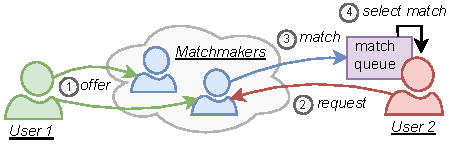
\includegraphics[width=\linewidth]{match/assets/matching_protocol_1}
		\caption{Order creation and dissemination.}
		\label{fig:matching_protocol_1}
	\end{subfigure}\vspace{0.5cm}
	\begin{subfigure}{.45\columnwidth}
		\centering
		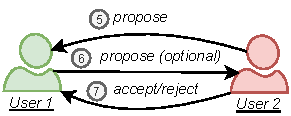
\includegraphics[width=\columnwidth]{match/assets/matching_protocol_2}
		\caption{Order negotiation.}
		\label{fig:matching_protocol_2}
	\end{subfigure}\vspace{0.5cm}
	\begin{subfigure}{.65\columnwidth}
		\centering
		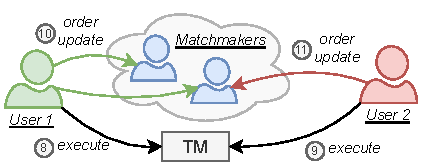
\includegraphics[width=\columnwidth]{match/assets/matching_protocol_3}
		\caption{Match execution and order updates}
		\label{fig:matching_protocol_3}
	\end{subfigure}
	\caption{High-level overview of the MATCH protocol and the message exchange between users and matchmakers.}
	\label{fig:match_data_flow}
\end{figure*}

\section{The MATCH Protocol}
\label{sec:protocol}
We visualize the MATCH protocol and the message exchange between users and matchmakers in Figure~\ref{fig:match_data_flow}.
The key idea behind our protocol is matchmakers only inform users about matches, and that users negotiate a trade directly with counterparties.
%In summary, the protocol proceeds as f.
First, users send new offers and requests to one or more matchmakers (\circled{1} + \circled{2}).
Matchmakers match incoming orders with existing orders in their order books and notify users about potential matches (\circled{3}).
Users aggregate potential matches of a specific order in a match queue.
Some period after receiving the first match for a specific order, a user starts to process matches in the associated match queue (\circled{4}), starting with the best match, and negotiates with the user behind the matched order (\circled{5} - \circled{7}).
When the negotiating parties reach a trade agreement (in other words, intend to fulfil their orders with each other), they execute the negotiated trade agreement by sending it to the TM (\circled{8} + \circled{9}).
The negotiating parties then inform the matchmakers about the executed trade so they can update the state of the affected orders accordingly (\circled{10} + \circled{11}).
The matchmakers are also informed about a negative outcome during the negotiation process.
If an order is still open, a user selects the next best item from the associated match queue, if it is non-empty, and initiates the next negotiation process.
This repeats until the match queue is empty or the order is completed.
The steps in the MATCH protocol are now further explained.

\begin{lstlisting}[language=json,firstnumber=1,float=b,caption=An order in a ride-hailing market (in JSON format).,label=lst:order_example]
{"timestamp": "2020-02-24T09:09:19+0000",
"type": "RIDE",
"timeout": 3600,
"is_offer": false, // request for transportation
"public_key": "82ae2f8f0c473cbdf63b920...",
"signature": "d54af87c8f8e6d917729d14...",
"identifier": 5,
"quantity": 1,
"data": {
"latitude": "40.712776",
"longitude": "-74.005974"
} }
\end{lstlisting}

\subsection{Order Creation}
\label{sec:order_creation}
In MATCH, users create new orders to indicate their willingness to buy or sell resources, services and assets.
Listing~\ref{lst:order_example} exemplifies the structure of an order in MATCH that specifies a transportation request in a ride-hailing market.
This order, in JSON format, includes the waiting location of the order creator in the \texttt{data} field.
The content of the \texttt{data} field is flexible and depends on the context in which the order is created.
It can contain many attributes and constraints that affect how the order is matched.
Each order has a \texttt{type} field which is a string value indicating the type of the order.
The order type is used by matchmakers to apply the right policies for validation and matching, and to store the order in the appropriate order book.
In Listing~\ref{lst:order_example}, the \texttt{RIDE} type indicates an order in a ride-hailing market.
Similarly, an order with type \texttt{EUR/USD} can indicate an order trading Euro for Dollar.
The \texttt{is\_offer} field is a flag that indicates whether the order is an offer or a request.
%An order contains the following fields: one or more attributes, the order creation timestamp, the order timeout, the public identity of the order creator, a digital signature, the type of the order (offer or request) and a unique identifier.
%To ensure a generic description of offers and requests, each order contains attributes, which are primitive data types such as numbers or text.
%In a ride-hailing market, created orders usually contain at least two numerical attributes that indicate the location of a driver or a passenger (in the form of a longitude and a latitude coordinate).
%This generic description of orders is also adopted by other systems in the domain~\cite{veit2003matchmaking}.
The identifier in an order is an integer value that indicates the position of the order in the sequence of all orders created by that user.
Together with the public key of the order creator, it uniquely identifies an order in the network.
The digital signature in an order allows matchmakers to verify its authenticity.
Inclusion of the \texttt{timeout} value prevents orders from being included in order books for an indefinite amount of time.
Finally, each order has a quantity, which is an integer value that specifies the amount of assets, services or resources being offered or requested.
After creation, a user serializes the order in an \texttt{order} message and sends it to matchmakers.
%With the inclusion of the public identity of the order creator and a digital signature, others can verify the authenticity of new orders and incoming messages from the network.
%We assume that each peer involved in the MATCH protocol owns a digital key pair, used when signing or verifying orders and messages.
%Moreover, we assume that digital signatures cannot be forged and that messages will eventually be delivered, if resubmitted often enough.

%A trader $ t $ creates a new order $ O $ as follows.
%First, $ t $ constructs either an \texttt{offer} or \texttt{request} message containing all fields of the order in serialized form, excluding its digital signature.
%$ t $ then signs the message, appends the signature to it, and sends it to one or more matchmakers.
%How $ O $ is exactly disseminated to matchmakers depends on the implemented order dissemination policy (see Section \ref{subsec:overlay_logic}).
%Upon reception of an incoming \texttt{offer} or \texttt{request} message, a matchmaker first validates the digital signature and the correctness of the order, according to a validation policy (Section \ref{subsec:overlay_logic}).
%If the incoming order is valid, it will be inserted in the order book of the matchmaker and immediately matched.

Users can cancel an open order, say $ O $, at any time by sending a \texttt{cancel} message with the identifier of $ O $ and its public key to matchmakers.
A \texttt{cancel} message for $ O $ should be sent to the same matchmakers as the \texttt{order} message that contained the description of $ O $.
Therefore, users keep track of the matchmakers to which they have sent an \texttt{order} message.
Upon reception of a \texttt{cancel} message, matchmakers remove the cancelled order from their order book.
%The MATCH protocol supports the cancellation of orders.
%When a matchmaker receives a \texttt{cancel} message for $ O $, it should remove $ O $ from its order book.

%\begin{figure}[t]
%	\centering
%	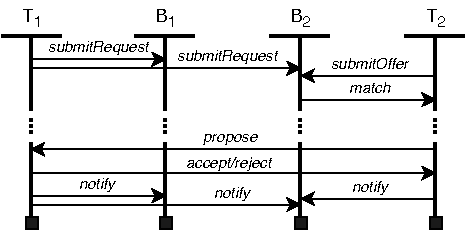
\includegraphics[width=\linewidth]{assets/sequence}
%	\caption{Sequence diagram of the messages exchanged between users and matchmakers in MATCH.}
%	\label{fig:match_sequence}
%\end{figure}

%\begin{figure*}[t]
%	\centering
%	\begin{subfigure}{.33\linewidth}
%		\centering
%		\includegraphics[width=.95\linewidth]{example-image-a}
%		\caption{Accuracy (adaptive $ f $)}
%		\label{fig:taxi_effectiveness_dynamic}
%	\end{subfigure}%
%	\begin{subfigure}{.33\linewidth}
%		\centering
%		\includegraphics[width=.95\linewidth]{example-image-b}
%		\caption{Bandwidth ($ f = 30 $)}
%		\label{fig:taxi_bandwidth_static}
%	\end{subfigure}%
%	\begin{subfigure}{.33\linewidth}
%		\centering
%		\includegraphics[width=.95\linewidth]{example-image-c}
%		\caption{Bandwidth (adaptive $ f $)}
%		\label{fig:taxi_bandwidth_dynamic}
%	\end{subfigure}
%	\caption{The influence of the network size, adversarial rate and message reach on the probability that a broker successfully match a compatible offer and request in MATCH.}
%	\label{fig:dissemination_strategy_experiments}
%\end{figure*}

\begin{figure}[t]
	\centering
	\includegraphics[width=.8\linewidth]{match/assets/matching_idea}
	\caption{The intuition behind order dissemination in MATCH.}
	\label{fig:matching_idea}
\end{figure}

\subsection{Order Dissemination}
\label{sec:order_dissemination}
%We now present the order dissemination model of MATCH.
In the replicated matchmaking model proposed in Section~\ref{sec:towards_fair_reliable_matchmaking}, a new order is disseminated to all matchmakers.
%This is not a scalable approach.
%Our replicated broker model discussed in Section \todo{X} assumes that each peer disseminates a new order to all available brokers.
We now address concern 2 from~Section~\ref{sec:towards_fair_reliable_matchmaking} and show how to considerably decrease the fanout of \texttt{order} messages (i.e., the number of matchmakers that a specific \texttt{order} message reaches) while still ensuring a high probability that a new order reaches a matchmaker with the current best matching order in their order book.
Specifically, we send a new order to a random subset of all matchmakers.
%Figure \ref{fig:matching_idea} illustrates the intuition behind this idea.
Let $ R_{req} $ and $ R_{off} $ indicate the sets of matchmakers that receive a specific request and offer, respectively.
The probability that at least one matchmaker will receive both a specific offer and request quickly goes to one, even when the order fanout is low compared to the number of matchmakers, also see Figure~\ref{fig:matching_idea}.
This phenomena is also known as the \enquote{birthday paradox} and is in practice exploited when computing hash collisions or when detecting a double spend attack in the Bitcoin network~\cite{schreiber2020k}.

Determining to how many matchmakers a new order is sent, is key.
In particular, we are interested in computing the probability that at least one matchmaker receives a matching offer and request.
If we consider a network with 1'000 matchmakers where new orders are disseminated to 50 matchmakers, this probability is given by $ \frac{1000-50}{1000} \cdot \frac{1000-50-1}{1000} \cdots \frac{1000-50-49}{1000} $.
%We indicate the set of matchmakers receiving a particular request and offer, as $ R_{req} $ and $ R_{off} $, respectively.
The probability that there is at least one matchmaker amongst all $ m $ matchmakers receiving both an offer and a request, with order fanout $ f $, is equal to:
%One of the problems of decentralized matchmaking is to ensure a sufficient amount of order duplication, while avoiding a network-wide dissemination of new orders (see Section \ref{subsec:problem_formulation}).
%Our solution is to send new offers and requests to $ f $ unique matchmakers, such that the probability that no matchmaker receives both this offer and request is low.
%We call $ f $ the order fanout.

\begin{equation}
P(R_{req} \cap R_{off} \neq \emptyset) = 1 - \mathlarger{\prod}_{i=0}^{f-1} \big(\frac{m - f - i}{m}\big)
\label{eq:dissemination}
\end{equation}

The value of $ P(R_{req} \cap R_{off} \neq \emptyset) $ quickly increases when $ f $ increases.
Even if $ m = 100'000 $ and $ f = 500 $ (i.e., orders are sent to only 0.5\% of all matchmakers), the probability that at least one matchmaker receives both a matching offer and a request, is already 97.7\%.
In this setting, it reduces the required fanout of an \texttt{order} message from 200'000 (when disseminating a new order to all matchmakers) to merely 1'000, thus significantly reducing the network traffic required for order dissemination.
%Figure \ref{fig:matching_idea} illustrates the intuition behind this idea.
%Applying the idea of Equation~\ref{eq:dissemination} requires an intuition on the total number of matchmakers, which can either be fixed by the software developers or be inferred using network estimation techniques~\cite{shames2012distributed}.
Note that the value of $ m $ is known to users in MATCH since they possess a list of all matchmakers.
Given a target value for $ P(R_{req} \cap R_{off} \neq \emptyset) $, users compute an appropriate fanout value themselves.
%In practice, the value of $ f $ should be tuned conservatively to account for network failures and matchmakers that are unreachable.
%Our evaluation (Section~\ref{sec:experiments}), we show that this dissemination strategy still results in a near-optimal matching of orders.

%Equation~\ref{eq:dissemination} assumes full network connectivity and an absence of adversarial brokers.
%Since these assumptions are unrealistic, we conduct simulations to better understand the properties of our order dissemination strategy when considering adversarial matchmakers.
%In particular, we experiment with the effects of the network size, fraction of adversarial matchmakers in the network and the reach of orders.
%These results are visualized in Figure~\ref{fig:dissemination_strategy_experiments}.\todo{explain}

\textbf{Malicious Matchmakers.}
Equation~\ref{eq:dissemination} assumes that all matchmakers in the set $ R_{req} \cap R_{off} $ follow the protocol and actually inform order creators when receiving matching orders.
This assumption violates our threat model since malicious matchmakers can respond with sub-optimal matches, or not respond with matches at all.
Therefore, we modify Equation~\ref{eq:dissemination} to account for the situation where a fraction $ r $ of all matchmakers is malicious.
Intuitively, this situation would require a higher value of $ f $ in order to reach at least one honest matchmaker.
%We adjust Equation~\ref{eq:dissemination} .
%We model a malicious matchmaker as a peer that does not respond to incoming offers and requests that match.
%Its behavior is therefore indistinguishable from being offline.
%This also accounts for the situation where a malicious matchmaker matches according to selfish interest, which can be considered as \enquote{invalid} matches.
Given a fraction of malicious matchmakers $ r $, $ P(R_{req} \cap R_{off} \neq \emptyset) $ is now equal to:

\begin{equation}
P(R_{req} \cap R_{off} \neq \emptyset) = 1 - \mathlarger{\prod}_{i=0}^{f-1} \big(\frac{(m - \left \lfloor{(1-r)f}\right \rfloor - i}{m}\big)
\label{eq:malicious_dissemination}
\end{equation}

%Equation~\ref{eq:malicious_dissemination} now accounts for matchmakers that are  who are not informing users about possible matches for their order, either intentionally (e.g., when hiding matches) or unintentionally (e.g., when the matchmaker has crashed).
We show in the next subsection that this is an appropriate modelling of malicious matchmakers.
The rationale behind this model is as follows.
The quality of matches from malicious matchmakers is likely to be lower compared to those received from honest matchmakers.
Therefore, there is a high probability that the effect of malicious matchmakers is negated upon receiving matches from an honest matchmaker, since a user will process the matches of honest matchmakers first.
Reaching honest matchmakers in the presence of malicious matchmakers requires a higher fanout value.

%A matchmaker immediately matches incoming, valid orders with existing ones in their order book.
%Orders are matched according to a matching policy, discussed in Section \ref{subsec:matching_engine}.
%For instance, in a ride-hailing market like Uber, a bid order created by a passenger is matched against only one ask order created by a driver.
When a matchmaker receives an \texttt{order} message describing an order $ O $, it matches $ O $ with existing orders in its order book with the same type, according to a matching policy (see Section~\ref{sec:architecture}).
For each order matched against $ O $, the matchmaker constructs a \texttt{match} message and sends it to the user that created $ O $ (step \circled{3} in Figure~\ref{fig:match_data_flow}).
A \texttt{match} message contains the full specifications of the matched orders, and the network address of the user behind the matched order.
This network address is used by the receiver of the \texttt{match} message to initiate the order negotiation process with the user behind the matched order.
%This message is then digitally signed by $ m $ and sent to the trader that initially created $ O $.\todo{why no reservation?}

%\begin{figure}[t]
%	\centering
%	\includegraphics[width=\linewidth]{assets/matching_idea}
%	\caption{Intuition behind the order dissemination strategy to brokers in MATCH.}
%	\label{fig:matching_idea}
%\end{figure}



%If the order fanout is relatively large (say $ f \geq 100 $), the message dissemination of \texttt{offer}, \texttt{request} and \texttt{CancelOrder} messages differs.
%Instead of sending a new message to $ f $ matchmakers directly, the message is first sent to some matchmakers, who then relay the message to other matchmakers.
%The number of hops that a message traverses is specified by a \emph{TTL} value included in the message.
%Upon receiving a new order from the network, the \emph{TTL} value is decremented by one and only forwarded if \emph{TTL} > 0.
%Our implementation supports gossiping-based message dissemination.

%We now present two basic order dissemination policies, based on the idea in Figure \ref{fig:matching_idea}.

%\textbf{Fixed broadcast (FIXEDBC)} - 
%The fixed broadcast policy, also called \texttt{FIXEDBC}, disseminates a new order to the same $ f $ unique matchmakers every time.
%This set should be fixed when a trader has discovered at least $ f $ matchmakers.
%The matchmakers selected by a trader that creates a large number of new orders have to receive and match incoming orders.
%Additionally, each broadcast order contains a \emph{TTL} value which indicates the maximum number of hops a new order traverses.
%Upon receiving a new order from the network, the \emph{TTL} value is decremented by one and forwarded if \emph{TTL} > 0.
%In this policy, load balancing is not as evenly spread as in the random broadcast policy: matchmakers withing \emph{TTL} hops of a trader that frequently submits orders will incur a higher load.

%The key difference between the random and neighborhood broadcast policies is that the destination set of orders in the latter policy is static.
%Subsequent orders, created by the same trader, should be inserted in the order books of the same matchmakers when neighborhood broadcast is used.


%\textbf{Random broadcast (RANDBC)} - 
%Under the random broadcast policy, also called \texttt{RANDBC}, traders send subsequent orders to $ f $ random, unique matchmakers every time.
%Assuming that these $ f $ matchmakers are uniformly sampled from the network, this policy has better load balancing properties since different matchmakers are selected each time traders broadcast a new order.
%This policy requires traders to discover more matchmakers when bootstrapping in the network, compared to the \texttt{FIXEDBC} policy.
%A potential trade off of this policy is matching effectiveness, since orders might not be matched in an optimal manner, depending on the matchmakers a specific order is sent to.
%We will discuss how to effectively pick the value of $ n $ further in this section.

\subsection{Match Queue}
\label{sec:match_queue}
Upon receiving a \texttt{match} message from a matchmaker, a user contacts the creator of the matched order and initiates a negotiation process (further discussed in Section~\ref{sec:order_negotiation}).
%After creating a new order, a trader can receive multiple \texttt{match} messages within a short period of time.
A potential strategy is that the user immediately contacts another user upon the arrival of a \texttt{match} message.
This possibly minimizes the time for an order to be completed.
However, this strategy leaves the user vulnerable to an attack where a malicious matchmaker is the first to send a specific \texttt{match} message to a user, which immediately triggers the negotiation process.
The quality of the received match described by the \texttt{match} message might be poor and the user might have received a match with a higher quality if it would have waited for additional matches from honest matchmakers.

\begin{figure*}[t]
	\centering
	\includegraphics[width=\linewidth]{match/assets/negotiation_diagram}
	\caption{The flow diagram (in UML format) when receiving a message during the negotiation process for a specific order.}
	\label{fig:order_negotiation_diagram}
\end{figure*}

To address this issue, incoming \texttt{match} messages for a specific order are first stored in a \emph{match queue}.
When a user receives the first \texttt{match} message for one of its offers (or requests), say $ O $, it creates a new match queue for $ O $.
Each entry in the match queue of offer (or request) $ O $ is a tuple $ (a, R) $ where $ R $ is a request (or offer) that matches with offer (or request) $ O $.
$ a $ indicates the number of failed negotiation attempts for $ R $.
The value of $ a $ is locally tracked by each user.
%The number of retries indicates how many times we unsuccessfully negotiated with the creator of $ O_2 $.
Removing items from the match queue is first based on $ a $ (item with a lower value of $ a $ have higher priority) and is then based on the quality of the match (the user prioritizes negotiation of matches with higher quality).
The quality of a match is an application-specific metric that can be considered as the \enquote{distance} between an offer and a request, and is computed by the matching policy.
An incoming \texttt{match} message can be inserted in multiple match queues, e.g., in the match queues for offers or requests with the same type and similar specifications.
%$ r $ is initially zero and is incremented by one each time trade negotiation fails (see Section~\ref{sec:order_negotiation}).
%Specifically, when a trader receives a \texttt{RejectTrade} message with this reason from the creator of $ O_2 $ during trade negotiation for his own order $ O_1 $, it adds the entry $ (r + 1, O_2) $ to the priority queue of $ O_1 $.
%Since a trading partner might have quantity reserved in their order that is released later, we try to send another trade proposal later in this situation.

%User store incoming \texttt{match} messages for a duration $ W_match $, after having received the first \texttt{match} message for a specific order.
Before a user starts to select items from a match queue, it waits for some duration $ W_{match} $, which we call the \emph{match window}.
The value of $ W_{match} $ should be carefully considered: a higher value of $ W_{match} $ increases the probability of receiving more and better matches but adds to the order completion time since a user has to wait longer before starting order negotiations.
Decreasing $ W_{match} $, however, might result in missing better matches.
$ W_{match} $ also depends on the link latency of the peer-to-peer network.
Furthermore, $ W_{match} $ is influenced by the trading domain, e.g., passengers in a ride-hailing market can usually tolerate an additional wait time of a few seconds, whereas this increase might be unacceptable when a user quickly wants to buy some assets in response to price fluctuations in an asset market.
When the match window expires, a user removes the entry $ (a, R) $ with the best quality from the match queue and initiates the order negotiation process with the user that created $ R $.
%Users prioritize the selection of items from the match queue first by the quality of the match, and then by $ r $.
%To prevent traders from sending out \texttt{ProposeTrade} messages at roughly the same time (and thus increasing load on individual traders), we introduce a small \emph{propose window} $ W_p $ which is a random duration between the removal of an entry from a match queue, and sending out a \texttt{ProposeTrade} message.
%Only when negotiation for an order fails or succeeds, the next entry is removed from the appropriate match queue, until the order is either canceled, expired or completed.
%If order $ O $ is completed, the match queue associated with $ O $ is deleted.

\subsection{Order Negotiation}
\label{sec:order_negotiation}

In MATCH, users negotiate about their orders with other users.
This negotiation approach increases resilience against malicious matchmakers since rational users choose to negotiate about the best incoming matches in order to get the best deal.
When two negotiating users reach a trade agreement, both users send the agreement to the TM, upon which the trade is executed.
This approach addresses question 1 in Section~\ref{sec:towards_fair_reliable_matchmaking} and avoids the need for network-wide consensus.

We now elaborate on the negotiation procedure between two users.
In the following, we assume that user $ U_1 $ created offer $ O $, user $ U_2 $ created request $ R $, and these two orders match.
Now, $ U_2 $ has received a \texttt{match} message from a matchmaker, informing $ U_2 $ about matching offer $ O $.
This puts entry $ (a, O) $ in the match queue associated with $ R $.
Order negotiation, based on match queue entry $ (a, O) $, starts by $ U_2 $ locking quantity in request $ R $.
How much quantity is locked depends on the available quantities in both $ O $ and $ R $.
Specifically, $ U_2 $ proposes to trade as much available quantity as possible, given the specifications of $ O $ and $ R $.
Explicitly locking quantity in an order prevents a user from engaging in parallel negotiations for the same resources.
MATCH does not enforce the locking of quantity since we assume that rational users will correctly manage their orders.
After locking the quantities in $ R $, $ U_2 $ sends a \texttt{propose} message to $ U_1 $, containing the full specifications of $ R $, the identifier of $ O $, and the proposed quantity to trade.

Figure~\ref{fig:order_negotiation_diagram} shows the control flow in UML format when a user receives specific messages during the order negotiation process.
We elaborate the negotiation process between users $ U_1 $ and $ U_2 $ according to Figure~\ref{fig:order_negotiation_diagram}.
When $ U_1 $ receives a \texttt{propose} message from $ U_2 $, it first checks if its offer $ O $, which identifier is contained in the \texttt{propose} message, is still open.
If $ O $ is expired, has been cancelled, or has been completed already, $ U_2 $ immediately responds with a \texttt{reject} message, containing the reject reason.
When $ U_2 $ receives the \texttt{reject} message from $ U_1 $, it unlocks the locked quantity for that negotiation and selects the next entry from the match queue of its request $ R $.
Since matchmakers might have outdated information about $ O $ (e.g., when $ O $ has been completed but the matchmaker has not been notified about this event), $ U_2 $ forwards the \texttt{reject} message to the matchmakers that informed $ U_2 $ about the match with $ O $.
Matchmakers then update the state of $ O $ accordingly when receiving a \texttt{reject} message.

If offer $ O $ is open, $ U_1 $ first determines if the incoming proposal is acceptable.
This step depends on the trading domain and specifically on the application-specific data in the order.
For example, a matchmaker in a ride-hailing market can establish a valid match between a passenger and driver.
However, this match might be unacceptable for one of the matched parties (e.g., when the geographic separation between the parties is too large).
If $ U_1 $ finds the proposal unacceptable, it sends a \texttt{reject} message to $ U_2 $.

If the proposal is acceptable, $ U_1 $ checks if it has any unlocked quantity in the offer $ O $.
If there is no unlocked quantity available for trade, $ U_1 $ responds with a \texttt{busy} message to $ U_2 $, indicating that it currently has no room for negotiation.
In this situation, $ U_1 $ is already engaged in negotiations for that order with other users.
Upon receiving a \texttt{busy} message, $ U_2 $ unlocks the locked quantity in $ R $ and re-adds the entry associated with the failed negotiation to the match queue of $ R $, incrementing $ a $ by one.
Re-adding this entry to the match queue will cause $ U_2 $ to initiate a negotiation with $ U_1 $ again later.
To prevent a user from immediately retrying a failed negotiation, a user waits a random period (between 1 and 2 seconds) before sending out another \texttt{propose} message when processing a match queue entry with $ a > 0 $.

If offer $ O $ has unlocked quantity, $ U_1 $ checks whether the full proposed quantity can be traded.
If so, $ U_1 $ sends an \texttt{accept} message to $ U_2 $, thereby accepting the proposal of $ U_2 $.
$ U_1 $ also forwards the \texttt{accept} message to the matchmakers that proposed the match so they can update the state of this order in their order book.
If the proposed quantity is unavailable in $ O $, $ U_1 $ makes a counter-proposal by locking as much quantity as possible in $ O $ and by sending a \texttt{proposal} message back to $ U_2 $ with this (lower) quantity.
$ U_1 $ and $ U_2 $ keep sending \texttt{propose} messages with differing quantities until one of them responds with either an \texttt{accept} or a \texttt{reject} message.

%During the second phase of the matching protocol traders negotiate a trade based on an incoming \texttt{match} message (see Figure \ref{fig:matching_protocol_2}).

%This phase starts when a trader, say $ t_1 $, receives a \texttt{match} message for its order $ O_1 $ from a matchmaker $ m $ that matched $ O_1 $ with another order $ O_2 $, created by $ t_2 $.
%When a trader receives a \texttt{match} message, it contact the trader behind the matched order directly, and try to negotiate a trade.
%This process is visualized in Figure \ref{fig:matching_protocol_2} and always involves the trader behind a matched ask and bid order.
%The recipient $ t_1 $ of a \texttt{match} message that matches order $ O_1 $ (created by $ t $) with another order $ O_2 $ (created by $ t_2 $) first checks whether his order is still open (since it could have been fulfilled already by other orders).
%If $ O_1 $ is expired, completed, or canceled, $ t_1 $ immediately sends a \texttt{DeclineMatch} message back to $ m $ and $ m $ then removes $ O_1 $ from its order book.
%Otherwise, $ t_1 $ reserves a part of (the assets, resources or services in) $ O_1 $ and sends a \texttt{ProposeTrade} message to $ t_2 $.
%This message contains full specifications of $ O_1 $ and a trade proposal with a quantity $ q $.
%During this phase, the sender digitally signs all their outgoing messages.

%When $ t_2 $ receives a \texttt{ProposeTrade} message from $ t_1 $, it first checks the status of its order $ O_2 $.
%If this order is expired, completed or canceled, $ t_2 $ immediately sends a \texttt{RejectTrade} message back to $ t_1 $.
%The same happens when there is no unreserved quantity available in $ O_2 $, e.g., when $ t_2 $ has an outstanding trade proposal with another trader.
%A \texttt{RejectTrade} message contains the reason why the trade proposal is rejected.
%If $ O_2 $ has at least $ q $ available quantity, $ t_2 $ sends an \texttt{AcceptTrade} message to $ t_1 $.
%Otherwise, if $ O_2 $ has available quantity but less than $ q $, $ t_2 $ can send a \texttt{CounterTrade} message to $ t_1 $, proposing an alternative quantity to trade.
%$ t_1 $ either accepts or rejects a counter proposal by responding with a \texttt{AcceptTrade} or \texttt{RejectTrade} message, respectively.
%At most, three messages are exchanged between $ t_1 $ and $ t_2 $ during this phase.
%At this point, $ t_1 $ and $ t_2 $ have either negotiated a trade, or one of the parties declined a trade proposal.

It could be that one of the involved parties does not respond during a negotiation, e.g., to deliberately lock quantity in the orders of another user.
%In this case, $ t_1 $ will never receive a response from $ t_2 $.
To address this situation, all outgoing messages during order negotiation have a fixed \emph{negotiation window}, indicated by $ W_{neg} $, after which the user leaves the negotiation.
When this window expires, any locked quantity for this negotiation is released and incoming messages regarding the expired negotiation are ignored.

%We prevent this by having a trader aggregate multiple incoming \texttt{matches} for the same order before sending out trade proposals.
%After receiving the first \texttt{match} message for a specific order, a trader waits for a fixed duration in seconds which we refer to as the \emph{matching window}, denoted by $ w $.
%A high value of $ w $ increases the probability of receiving good matches but delays the order completion process since one has to wait longer before sending out trade proposals.
%On the other hand, a small $ w $ might lead to missing better matches.

%\subsection{Avoiding Full Replication}
%TODO

%\section{The MATCH Protocol}
%\label{sec:protocol}
%To ensure correct order management (problem I), we design a three-phase protocol, named MATCH.
%We first briefly introduce the MATCH protocol and its phases, and then provide a more detailed description per phase.
%The design of the MATCH protocol is inspired by prior work of Raman et al., which proposes a related protocol to match resources and jobs in a centralized matchmaking environment~\cite{raman1998matchmaking}.

%In phase I, order creators submit new offers and requests to matchmakers and matchmakers notify these creators about potential trading parties with \emph{match notifications}.
%When receiving a match notification from a matchmaker, an order creator starts to negotiate directly with the matched party (phase II) and informs matchmakers about the outcome of the trade negotiation (phase III).
%Since order creators will collect incoming match proposals and process them accordingly, this protocol ensures correct behavior in the situation where multiple matchmakers match the same order.
%To prevent orders from being settled multiple times, matchmakers inform traders about potential trading partners, upon which traders start to negotiate a trade with the matched counterparty.\todo{why matchmaking at all?, pre-aggregate of information, exhaustive search}
%Since the creator behind an order will determine to which matches it responds and ensures their order is not fulfilled multiple times, different matchmakers can propose the same match to this order creator simultaneously. % it addresses the problem where the same order is matched by multiple matchmakers.

%We embed this  embedded in the design of the MATCH protocol, visualized in Figure \ref{fig:matching_protocol}.
%First, traders send new orders to matchmakers and  matchmakers match the orders of two traders.
%Next, a trader that is informed about a potential match directly contacts the matched counterparty and proposes to trade.
%When the trade is finished, the involved parties notify the matchmaker and their order books are then updated accordingly.

\subsection{Match Execution and Order Updates}
Upon reaching a trade agreement between two negotiating users, it should be executed by the trading mechanism.
To execute a trade agreement, one party sends the \texttt{propose} message to the TM and the other party sends the \texttt{accept} message to the TM (step \circled{8} and \circled{9} in Figure~\ref{fig:match_data_flow}).
Each message contains the digital signature of its creator.
The TM executes the trade after having received both these messages.
%Both users then internally update their order.
Next, each involved party individually inform the matchmakers that originally received their order about the match execution by sending an \texttt{update} message (step \circled{10} and \circled{11} in Figure~\ref{fig:match_data_flow}).
This message contains the order with an updated quantity, specifying the new interests of the order creator after the match has been executed.
The \texttt{update} message contains an order with quantity 0 if it has been completed.
%When $ t_1 $ and $ t_2 $ agree to trade, the trade should be executed by actually exchanging assets, services or resources.
%We assume that a negotiated trade is executed by an application-specific trading mechanism (its specifications are discussed in Section \ref{subsec:trading_mechanism}).
%When a trade has successfully been executed between $ t_1 $ and $ t_2 $, both parties notify the original recipients of the \texttt{offer} or \texttt{request} messages that contained $ O_1 $ or $ O_2 $, by broadcasting a signed \texttt{TradeComplete} message.
%A \texttt{TradeComplete} message contains full specifications of both orders, and the details of the executed trade between $ t_1 $ and $ t_2 $.
%Both $ t_1 $ and $ t_2 $ broadcast a \texttt{TradeComplete} message to the matchmakers where they initially sent their \texttt{ask} or \texttt{bid} message to.
Upon receiving an \texttt{update} message, matchmakers update the state of the changed order accordingly and remove orders that have been completed.

%If trade negotiation has failed or a trade proposal did time out, one of the involved parties (either $ t_1 $ or $ t_2 $) notifies the matchmaker $ m $ about the outcome by sending a \texttt{DeclineMatch} message, containing the reason of the failed trade negotiation.
%If a \texttt{DeclineMatch} message indicates that either $ O_1 $ or $ O_2 $ is completed, canceled, or expired, $ m $ removes this order from their order book.
%A \texttt{DeclineMatch} message is also sent back to $ m $ if the actual trade fails for reasons specific to the trading mechanism (see Section \ref{subsec:trading_mechanism}).

%\subsection{Order Book Synchronization}
%In MATCH, matchmakers periodically synchronize orders in the order book with other matchmakers.
%We refer to the duration between subsequent synchronizations of a single matchmaker as the \emph{synchronization window} $ W_{sync} $.
%A matchmaker $ m_1 $ synchronizes their order book with matchmaker $ m_2 $ as follows: periodically, $ m_1 $ sends a \texttt{sync} message to a random other matchmaker, say $ m_2 $.
%This message contains a Bloom filter $ B $, initialized with the identifiers of all offers and requests in the order book of $ m_1 $.
%The false positive rate of $ B $ is fixed to 5\%.
%When $ m_2 $ receives a \texttt{sync} message, it iterates over all offers and requests in its order book and assembles a set with order identifiers that have no membership in $ B $.
%To avoid synchronization of the entire order book, $ m_1 $ samples a random subset with $ b $ orders, where $ b $ is called the synchronization batch size.
%Upon reception of $ B $, $ m_2 $ sends up to $ b $ individual \texttt{order} messages to $ m_1 $.

%Which orders are being synchronized depends on an \emph{synchronization policy}.\todo{to BF or not to BF?}

%A matchmaker that wants to synchronize their order book with another peer first sends a message that contains two bloomfilters: one filled with the IDs of active orders in the order book, and another one that is filled with the IDs of canceled orders.\todo{why cancelled orders?}
%The receiving party now sends missing orders to the initiating party.

%\textbf{No synchronization} -
%While (periodic) order synchronization potentially increases matching effectiveness, the additional communication outweighs the increased matching effectiveness in specific situations.
%For example, order synchronization is less effective when a new order is already disseminated to a significant fraction of all matchmakers.
%Therefore, we also consider a policy where orders are not synchronized at all.
%No synchronization reduces communication costs but potentially leads to the miss of better matches.

\section{The MATCH Middleware Architecture}
\label{sec:architecture}
We now present the MATCH middleware architecture, visualized in Figure~\ref{fig:matching_architecture}.
Each user and matchmaker deploy a single instance of the MATCH middleware as a shared runtime library.
Communication with the middleware by external applications proceeds through an API, which specifications are included in our open-source implementation.
We now elaborate on the components in the MATCH middleware architecture.
%We now present the architecture of MATCH, our distributed order matching mechanism.
%The overall architecture and information flow is presented in Figure \ref{fig:matching_architecture}.
%We briefly elaborate on the individual components.

\textbf{Network layer.}
The network layer passes incoming messages to the MATCH overlay logic and routes outgoing messages to their intended destination.
This layer can be implemented using any networking library with support for peer-to-peer communication and authenticated messaging.
%We should note however that further optimizations can be made in network topology, depending on the domain to which MATCH is applied.
%This lowers generality and re-usability.
%The network has a random topology and each peer $ p $ maintains a connection to $ i $ other random peers.

\begin{figure}[t]
	\centering
	\includegraphics[width=.9\linewidth]{match/assets/matching_architecture}
	\caption{The MATCH middleware architecture.}
	\label{fig:matching_architecture}
\end{figure}

\textbf{Overlay logic.}
The overlay logic processes incoming messages received by the network layer. %, such as new orders, matches and received from the network. % various routines that execute when a specific message is received.
It inserts incoming \texttt{match} messages in the appropriate match queue, discussed in Section~\ref{sec:match_queue}.
It contains policies for order \emph{validation} which specify how the validity of an incoming order with a given type is determined.
The validation policy takes into consideration the attributes in the \texttt{data} field of the order (see Listing~\ref{lst:order_example}), and checks whether they are valid with respect to a trading domain.
For example, a validation policy for orders in a ride-hailing market should check whether the latitude and longitude coordinates are included and within a valid range (-90 to 90).
We envision that developers share the implementation of these policies through some distribution medium (e.g., a website).
To increase the trustworthiness and security of these policies, the policy implementations should be auditable and attestable by other developers and auditors.
These validation policies can then downloaded by users and matchmakers that are interesting in participation within a specific trading domain.
We provide developers the means to create custom validation policies, enabling order validation in different trading contexts.
Incoming orders deemed invalid by the validation policy are discarded and not processed.

%New incoming orders received by overlay logic are first checked for validity; if valid they are dispatched to both the order book (so they can be inserted) and the matching engine, which attempts to find matches for this new order.

\textbf{Order books.}
Each matchmaker can host multiple order books, coloured green in Figure~\ref{fig:matching_architecture}, which store orders with differing types.
For example, MATCH can maintain an asset trading order book that stores orders to buy or sell Euros for Dollars, and another ride-hailing order book that stores transportation requests and ride offers.
Maintaining multiple order books is a key property of MATCH and results in a single and reusable matchmaking solution that can be deployed across different domains.
%New order books are created on demand, based on the type of incoming orders.

\textbf{Matching engine.}
Valid incoming orders are passed to the matching engine, coloured red in Figure~\ref{fig:matching_architecture}.
The matching engine attempts to match incoming offers and requests with existing requests and offers, respectively.
It contains \emph{matching policies} which predicate whether a specific offer and request match, based on the order type and specifications.
%It takes a buy and a sell order as input and determines whether there is a match, based on one or more attributes of these orders.
For example, matchmaking in a ride-hailing market is often based on the geographic distance between a driver and a passenger.
Likewise, asset orders would match if the price of an offer is equal to or lower than the price of a request.
Similar to validation policies, matching policies are published on a website or on another public medium, and can be downloaded by interested matchmakers.
%Matchmaking can also be based on multiple, weighted attributes.
%A match found by the matching engine is passed to the overlay logic, converted into a \texttt{match} message, and send to the order creator.

\textbf{Negotiation stores.}
To correctly process incoming messages from negotiation counterparties, MATCH requires state storage of outgoing messages during order negotiation.
This state is stored in a \emph{negotiation store}, coloured yellow in Figure~\ref{fig:matching_architecture}.
For each negotiation, a new negotiation store is created, a unique identifier is generated, and this identifier is appended to each message associated with this negotiation.
Counterparties are required to include the same identifier in response messages.
Incoming negotiation messages containing an unknown identifier are discarded by users.
Negotiation stores time out after the negotiation window expires, on which the store and its contents are deleted.
%On timeout, the negotiation store is deleted and the overlay logic is notified about this event.

\textbf{Trading mechanism.}
Negotiated trade agreements are passed to the trading mechanism that executes the trade.
We consider this component external to MATCH.
%The trading mechanism requires the implementation of the \texttt{startTrade($ O_1, O_2, q $)} function which expects the two matched orders $ O_1 $ and $ O_2 $, and the agreed quantity to trade ($ q $) as arguments.
The trading mechanism notifies the overlay logic when the trade is executed.
This notification includes one or more transaction identifiers and a boolean value indicating whether the trade was successful or not.
We assume that the trading mechanism provides atomic guarantees: either the full negotiated match is executed or nothing is being executed.
This guarantee is, for example, provided by smart contracts, applications that runs on top of a blockchain (also see Section~\ref{sec:experiments_ethereum})~\cite{luu2016making}.
%The trading mechanism the notifies the overlay logic with the outcome of the trade.
%We consider three different trade outcomes: succeeded, when all assets have successfully been exchange between two parties, or failed, when an error occurred during the trading process.
%The trade outcome is then broadcast to matchmakers (see phase III in Section~\ref{subsec:protocol_phase_3}).

%\section{Model and Formalisms}
%MATCH is middleware that interacts with a peer-to-peer network and market trading mechanism.
%Prior to presenting the architecture of MATCH and the matching protocol, we discuss the model of our peer-to-peer network and trading mechanism.
%We start by defining the specifications and assumptions of the network layer and trading mechanism.
%Next, we formally define the data structures that MATCH requires, including orders, the order book and the matching function.
%These definitions will guide the design of our matchmaking protocol.

%\subsection{Trading Mechanism Model}
%We assume that there is a trading mechanism that handles the execution of a trade between two participants.
%The trading mechanism handles the trading process after two orders have been matched, and ensures that resources, services or assets between the entities that created the matched orders, are traded.
%This process might be executed by one or more centralized entities, e.g. financial institutions that transfers funds from one party to another.
%We assume that the asset exchange mechanism used in the market mechanism is secured against fraud.
%This could for instance be achieved by using atomic swaps where assets are exchanged between blockchain ledgers in a secure and atomic manner. %or a trusted central settlement institution.


%\subsection{Data Structures}
%The goal of MATCH is to match incoming orders in a decentralized manner.
%To keep our mechanism applicable in many market contexts, we specifically do not make assumptions about the content of individual orders.
%We now formally define various data structures which MATCH uses.
%MATCH is built to act as middleware between a peer-to-peer network and a trading mechanism.
%More specifically, we assume a trading environment where assets are being traded.

%First, we provide the definition of an asset.
%An asset represents either a tangible or intangible object with some value, e.g. some dollars, stocks or a taxi ride.
%We formally define an asset as follows:

%\begin{mydef}
%	(Asset) An asset $ A $ is defined as a pair $ (ID, A) $ where $ ID $ is a unique serializable identifier that represents the type of the asset and $ A = (a_1, a_2, ... a_n) $ denotes a set of $ n $ attributes.
%\end{mydef}

%In the context of stock trading, we can define a specific quantity of assets as $ (AAPL, \{amount=23\}) $ to indicate 23 stocks with the $ AAPL $ symbol.
%While an asset might intuitively be thought of as some physical or digital good, we can use Definition X to also model resources or services as assets.
%For example, a service request for transportation to a remote location in a ride-hailing market can be modelled as $ (RIDEREQ, \{pickup=(1, 2), dropoff=(1,2)\}) $.
%The methodology of modelling tangible and intangible assets or resources as digital tokens is a commonly adopted concept within various blockchain-based marketplaces. % approach is very  the "tokenization" of both tangible (physical) and intangible assets.

%In most electronic markets, two types of assets are being exchanged between traders, e.g. two types of currencies.
%Before we define what comprises an order in MATCH, we must first define an asset pair.

%\begin{mydef}
%	(Asset pair) An asset pair $ P = (A_1, A_2) $ is an ordered pair of two assets $ A_1 $ and $ A_2 $ where $ A_1.id $ is lexicographically smaller than $ A_2.id $.
%\end{mydef}

%We can now model the specifications of an asset exchange between two trades as an asset pair.
%For example, if a trader wants to sell 23 stocks of the AAPL symbol for a price of \$40 each, we can model this with the asset pair $ ((AAPL, \{amount=23\}), (EUR, 920)) $.
%With the definition of an asset pair, we can now formalize an order.

%\begin{mydef}
%	(Order)
%	An order $ O_t $ created by trader $ t $ is defined as a tuple $ (P, t_{pk}, i) $ where $ P $ is an asset pair, $ t_{pk} $ the public key of trader $ t $, $ i $ indicates the timeout of the order in milliseconds.
%\end{mydef}

%We now make the distinction between ask (sell) orders and bid (buy) orders.

%\begin{mydef}
%	(Ask order) An ask order $ A_t $ created by trader $ t $ is a sell order $ O_t $ where $ t $ intends to exchange $ O_t.P.A_1 $ for $ O_t.P.A_2 $.
%\end{mydef}

%\begin{mydef}
%	(Bid order) A bid order $ A_t $ created by trader $ t $ is a buy order $ O_t $ where $ t $ intends to exchange $ O_t.P.A_2 $ for $ O_t.P.A_1 $.
%\end{mydef}

%Recall that we restricted an asset pair to be ordered in Definition X.
%This is explicitly done to avoid symmetric orders.
%To elaborate, an ask with asset pair $ (A_1, A_2) $ is equivalent a bid with asset pair $ (A_2, A_1) $.
%To avoid duplication in the market, we enforce an order within the asset pair.

%Matchmakers organize known ask and bids within an \emph{order book}, which we formally define in the following definition.

%\begin{mydef}
%	(Orderbook) An order book $ B_{t1, t2} $ is defined as a set $ \{ O_1, O_2, ... O_n \} $ of $ n $ orders. We denote the size of order book $ B $ as $ |B| $.
%\end{mydef}

%Note that each order has a timeout.
%This attribute is included to prevent orders from being open for an indefinite amount of time and potentially polluting order books across the network.
%In addition, each order is digitally signed by its creator.
%This prevents other traders from creating orders under a different identity.

%Figure \ref{fig:order_book} shows an example of an order book used in a stock trading market, with three bid orders and three ask orders.
%When presenting an order book to traders, ask and bid orders are usually sorted, i.e. based on their price.
%For orders with a price, ask orders are sorted ascending on price and bid orders descending on price in the order book (the best orders are presented first).

%When a trader receives a new ask or bid from the network, it attempts to match this new order with existing orders in the order book.
%We now define a generic matching function, that takes a new order and order book as input, and output a set of orders that match.

%\begin{mydef}
%	(Matching function) A matching function $ M: (O, B) \rightarrow  $ returns matching ask or bid orders in an order book $ B $ for a new incoming bid or ask order respectively.
%\end{mydef}

%At this point, we should remark that the matching function highly depends on the type of assets being traded.
%The matching function usually takes in consideration one or more attributes of the assets defined in the order, e.g. a price in the context of stock trading or a pickup location when matching passengers and drivers a ride-hailing market.
%To illustrate this, assume that a new bid order arrives with a price of \$149.58 and with an amount of 800, and is matched against the content of the order book presented in Figure \ref{fig:order_book}. %, when a new bid order is submitted to the order book in Figure \ref{fig:order_book} , it will be matched with the following ask orders.
%Now, this bid order will be fully matched against the ask orders with ID \#7829 and ID \#7828 and the ask order with ID \#7820 will be partially matched for an amount of 104.
%When two or more orders are matched, their order book entries are updated or they are removed from the order book if the order is fulfilled.

%\section{Implementation Details}
%\label{sec:implementation}
%Request stores are organized in a dictionary with the request identifiers as keys and the individual request stores as values.
%The matching priority queue is implemented as a linked list that remains sorted whenever new entries are added to it.
%Different order books are organized in a dictionary whose keys are the order types, and the values are the individual order books.
%We provide both an implementation of a basic order book and a limit order book, optimized to store orders with pricing information.
%The basic order book structure contains two distinct sets with offers and requests, and can be used to store and match orders with any type of attributes.


%It matches orders first based on price, and then on time since order creation, while prioritizing orders that have been open for a longer time.
%Programmers can add custom matching policies by subclassing the \texttt{MatchPolicy} class and providing an implementation of the \texttt{match(order, order\_book)} method, which takes the order and a order book as parameters, and returns a set of matching orders.
%We provide a basic order validation policy that checks whether an incoming order has not expired yet and is not canceled already.
%Programmers can define advanced validation policies by subclassing the \texttt{ValidationPolicy} class and implementing the \texttt{isValid(order)} method, which takes the order to be validated as parameter and returns a boolean value.

%When a trader broadcasts a new order in the network, they can potentially receive a significant number of \texttt{match} messages within a short period of time, in particular when the order matches with multiple other ones, and the order fanout is large.
%To prevent a high load on a trader, we wait for a random duration between 0 and 1 second before sending an outgoing trade proposal to another trader the first time.
%Subsequent trade proposals to the same trader are queued for a duration between 1 and 2 seconds.
%Depending on the connectivity of the underlying peer-to-peer network, the wait duration might be increased.

%We now present various policies that specify how new orders are sent to matchmakers, and how existing orders are synchronized amongst them.
%In this section, we distinguish between \emph{synchronization} and \emph{dissemination} policies, and discuss each policy type in a separate section.

% Policies:
% - smart broadcast of new order
% - send new order to random matchmakers

% - neighbour sync
% - active sync amongst matchmakers + rand. walk
%

\begin{table}[t!]
	%\footnotesize
	\centering
	\begin{tabular}{|c|c|}
		\hline
		\textbf{Notation} & \textbf{Variable Description} \\ \hline
		$ W_{match} $ & Match window (fixed to 2 seconds) \\ \hline
		$ W_{neg} $ & Negotiation window (fixed to 5 seconds) \\ \hline
		$ m $ & Number of matchmakers \\ \hline
		$ f $ & Order fanout \\ \hline
		$ r $ & Fraction of malicious matchmakers \\ \hline
	\end{tabular}
	\caption{An overview of the variables used in Section~\ref{sec:experiments}.}
	\label{table:experiment_parameters}
\end{table}

\section{Experimental Evaluation}
\label{sec:experiments}
We implement the MATCH protocol and middleware in the Python 3 programming language, spanning a total of 6.511 lines of source code (SLOC), without comments.
The implementation uses the \texttt{asyncio} library for asynchronous event processing.
The network layer is implemented using our networking library, optimized for building peer-to-peer overlay networks and with built-in support for Network Address Translation (NAT) puncturing and authenticated messaging.\footnote{See \url{https://github.com/tribler/py-ipv8}}
For efficiency, message exchange between users and matchmakers uses UDP.
Order negotiation proceeds using TCP since this flow requires bilateral and reliable message exchange.
All software artifacts of MATCH (source code, tests, and documentation) are available online.\footnote{See \url{https://github.com/Tribler/anydex-core/tree/match-middleware20}}

In Section~\ref{sec:taxi_experiments} and~\ref{sec:asset_trading_experiments}, we subject the MATCH middleware to two workloads for ride-hailing and asset trading, reconstructed from real-world traces.
These experiments demonstrates that MATCH maintains high matching quality, is resilient against malicious matchmakers, and is reusable across different trading domains.
In Section~\ref{sec:experiments_ethereum}, we compare our solution to matchmaking on an Ethereum blockchain and show that MATCH uses considerably less bandwidth and has superior order fulfil latencies.
%Afterwards, we provide a summary with recommendations for each policy and their performance with regard to various system properties.

\begin{figure*}[t]
	\centering
	\begin{subfigure}{.5\columnwidth}
		\centering
		\includegraphics[width=\linewidth]{match/assets/plots/taxi_quality.pdf}
		\caption{Matching quality w. different fanouts $ f $}
		\label{fig:taxi_quality}
	\end{subfigure}%
	\begin{subfigure}{.5\columnwidth}
		\centering
		\includegraphics[width=\columnwidth]{match/assets/plots/taxi_fairness_fixed.pdf}
		\caption{Impact of selfish matching ($ f = 50 $)}
		\label{fig:taxi_fairness_fixed}
	\end{subfigure}\vspace{0.3cm}
	\begin{subfigure}{.5\columnwidth}
		\centering
		\includegraphics[width=\columnwidth]{match/assets/plots/taxi_fairness_adaptive.pdf}
		\caption{Impact of selfish matching (adaptive $ f $)}
		\label{fig:taxi_fairness_adaptive}
	\end{subfigure}
	\caption{The matching quality and impact of selfish matching when executing the ride-hailing workload in MATCH, while varying the number of matchmakers. In Figure (b) and (c), the order fanout $ f $ is either fixed  ($ f = 50 $) or adaptive such that $ P(R_{req} \cap R_{off} \neq \emptyset) \geq 0.95 $.}
	\label{fig:taxi_experiments}
\end{figure*}

%\subsection{Experimental Setup}
All experiments are conducted on our nation-wide university cluster, allowing us to run multiple instances of MATCH on different compute nodes~\cite{bal2016medium}.
It contains 48 compute nodes, each one equipped with dual 8-core E5-2630v3 CPU and 64GB of memory, running CentOS 6.
%More detailed specifications of the hardware and runtime environment are found online.
%On each compute node, we run at most 150 instances of MATCH when experimenting with the ride-hailing workload, and at most 64 instances under the asset trading workload (the latter workload results in a higher load on each compute node).
%We create a \emph{scenario} file which lists all operations that a peer executes during the experiment, e.g., order creation and cancellation.
To account for network latencies, we source a distribution from the PlanetLab latency dataset and uniformly sample from it when sending messages~\cite{zhu2016network}.
This also accounts for runtime variability of latency present in real-world networks.
Table~\ref{table:experiment_parameters} summarizes the variables that are used in this section.
The negotiation window ($ W_{neg} $) is fixed to five seconds, which is well above the highest observed round-trip time in the PlanetLab latency dataset.
The match window ($ W_{match} $) is fixed to two seconds.
These values should be increased when MATCH is deployed in networks with higher link latency, since it then can take longer for \texttt{match} or negotiation messages to arrive.
%We run each experiment at least five times (except for the load balancing and order fulfillment latency experiments) and average the results.
%Similar to the notation in Section~\ref{sec:order_dissemination}, in the following we use $ m $ to indicate the total number of matchmakers, $ f $ to indicate the order fanout, and $ r $ to indicate the fraction of malicious matchmakers.

%\begin{table}[t!]
%	\centering
%	\begin{tabular}{|c | c | c|} 
%		\hline
%		\textbf{Parameter Name} & \textbf{Ride-hailing} & \textbf{Asset trading} \\ \hline
%		Population ($ n $) & 2100 & 1000 \\ \hline
%		Matchmakers ($ m $) & 1100 & 1000 \\ \hline
%		Order fanout ($ f $) & 30 & 30 \\ \hline
%		Sync. interval ($ i $) & 30 sec. & 30 sec. \\ \hline
%		Sync. batch size ($ b $) & 10 orders & 10 orders \\ \hline
%		Match window ($ W_m $) & 2 sec. & 2 sec. \\ \hline
%		Propose window ($ W_p $) & 0 & $ W_p \sim U(0, 1) $ \\
%		\hline
%	\end{tabular}
%	\caption{Default experiment parameters for the ride-hailing and asset trading workloads.}
%	\label{table:experiment_parameters}
%\end{table}

\subsection{Ride-hailing Experiments}
\label{sec:taxi_experiments}
Unfair matchmaking in ride-hailing markets is a prominent threat to both drivers and passengers~\cite{bokanyi2019ride,calo2017taking}.
%Ride-hailing, popularized by companies like Uber and Lyft, is currently one of the largest peer-to-peer markets~\cite{kooti2017analyzing}.
We leverage the MATCH middleware to devise a decentralized alternative to ride-hailing platforms like Uber and Lyft. % where drivers perform fair matchmaking themselves. %, even when a subset of drivers match with selfish interest.
In this market, drivers perform matchmaking themselves.
The first set of experiments focuses on the matching quality and fairness of MATCH in a ride-hailing environment.
The used workload contains temporal information about ride offers and requests created by drivers and passengers, respectively.
Each order in the workload has a quantity of one, ensuring that a ride request is matched with at most one ride offer.

\textbf{Workload specification.}
The workload is reconstructed from historical traces of taxi rides published by the government of New York~\cite{tlc2017nyc}.
We analyse the traces and subtract 2'100 ride offers and requests during the busiest period in 2015: November 1, 00:59:57 to November 1, 01:01:16 (datasets published after 2015 did not include geographic information on drivers and passengers).
We assume a total of 1'100 drivers and 1'000 passengers, to resemble the situation where drivers are waiting idly for passengers.
First, drivers indicate their willingness to transport passengers by creating offers containing their waiting location, during 55 seconds (we wait 50 milliseconds between the creation of subsequent ride offers).
After this period, passengers submit requests containing their pick-up location, during almost 77 seconds.
After all passengers have submitted their request, we leave the experiment running for an additional 60 seconds, to ensure that all requests are matched with an offer.
Since the workload does not provide information on the identity of individual passengers or drivers, it is assumed that each passenger creates one request throughout the experiment. %, which is matched with one ride offer.
This assumption does not lead to skewed results since a passenger does not create multiple ride requests within short time~\cite{pham2017oride}.

For the this workload, we implement the matching policy such that it minimizes the distance between passengers and drivers, to reduce waiting times for passengers.
Specifically, the policy computes the geographic (haversine) distance between the locations included in offers and requests.
In this market, we define the matching quality as the average distance between matched passengers and drivers, which we also call the \emph{match distance}.
%We believe this is an adequate metric since it is directly correlated with the total distance that drivers have to traverse, which we aim to minimize.
This quality metric is also used by related work on matchmaking in ride-hailing markets~\cite{pham2017oride}.
%Matching is based on the great-circle distance between a driver and a passenger.
%Note that matching is one-to-one: each ride request is matched with exactly one ride offer.

\textbf{Matching quality.}
We first quantify the matching quality of MATCH under the ride-hailing workload when increasing the number of matchmakers for different values of the order fanout, see Figure~\ref{fig:taxi_quality}.
The horizontal axis shows the number of matchmakers ($ m $) and the vertical axis denotes the average match distance.
For this experiment, all matchmakers act honest and execute the same matching algorithm (in other words, $ r = 0 $).
As a baseline, we use the matching quality of a centralized matchmaking approach where a single server matches incoming orders in a FIFO manner (following the model in Figure~\ref{fig:central_exchange_architecture}).
This centralized approach results in an average match distance of 0.544km, and is indicated with a dashed horizontal line in the graphs of Figure~\ref{fig:taxi_experiments}.
%The horizontal axis denote the number of matchmakers and the vertical axis shows the matching effectiveness in terms of average matching distance in kilometers.
Figure \ref{fig:taxi_quality} shows that the average match distance increases when there are more matchmakers under a fixed order fanout.
Also, the match distance increases when the order fanout decreases.
In particular, It becomes less likely that (good) matches for offers and requests are found when either the number of matchmakers increases or the order fanout decreases.
The match distance increases significantly when $ f = 30 $ and $ m $ increases. E.g., for $ m = 2'000 $, the average match distance increases to 0.607km, 9.5\% higher compared to the baseline.
%For $ m = 2'000 $ and $ f = 60 $, each ride request required \todo{X} negotiations on average.

Remarkably, for lower values of $ f $ and $ m $, \emph{MATCH outperforms the performance of centralized matchmaking, in terms of matching quality.}
We explain this behaviour as follows.
With our ride-hailing workload, centralized matchmaking can immediately match a ride request with a ride offer.
The overall match quality, however, might be improved when batching incoming ride requests, since it could have been better to assign an already-matched driver to a passenger that created its request later during the experiment.
Call markets, for example, operate in batches, where incoming orders are first aggregated over time and then matched at predetermined time intervals.
In MATCH, users aggregate potential matches during the match window, $ W_{match} $, resembling this behaviour.
Therefore, the matching quality in MATCH can exceed that of centralized FIFO matchmaking because of match aggregation by users, at the cost of a larger order fulfil time.

\textbf{Impact of selfish matching.}
We show how selfish behaviour of malicious matchmakers impacts the matching quality.
We model a malicious matchmaker as a driver that matches an incoming ride request from a passenger with its own service offer first.
This captures the economic incentive of drivers to prioritize their own ride services.

Figure~\ref{fig:taxi_fairness_fixed} shows the average match distance under a fixed order fanout ($ f = 50 $) when increasing the number of matchmakers.
We vary $ r $, up to 75\% of all matchmakers ($ r = 0.75 $).
Figure~\ref{fig:taxi_fairness_fixed} shows that increasing both $ m $ and $ r $ has a negative impact on the matching quality in MATCH.
The problem is that a malicious matchmaker matches the requests of passengers with its own offer, while it likely would have established a better match if the matchmaker would have been honest.
Therefore, we also consider an adaptive order fanout, based on the values of both $ r $ and $ m $.
Specifically, $ f $ is fixed to the lowest integer value such that $ P(R_{req} \cap R_{off} \neq \emptyset) \geq 0.95 $.
Figure~\ref{fig:taxi_fairness_adaptive} visualizes these results with an adaptive order fanout.
The order fanout is 63 with $ m = 2'000 $ and $ r=0 $.
Formula~\ref{eq:malicious_dissemination} describes that when 50\% of the matchmakers prioritize their own ride offer ($ r=0.5 $), the order fanout increases to 78.
Figure~\ref{fig:taxi_fairness_adaptive} shows that the average match distance remains largely the same, even when increasing the total number of matchmakers.
These results show that in a network with 2'000 matchmakers, by increasing the order fanout by only 15, MATCH can tolerate with 50\% of all matchmakers acting maliciously and still produce a matching quality that is on par with the situation where all matchmakers are honest.
%We remark that by sending an order to 15 additional matchmakers in a network with 2'000 matchmakers, and with 50\% of these matchmakers acting malicious, MATCH still achieves a matching quality comparable to that of a centralized matchmaking approach.
In practice, the exact value of $ r $ is not known a-priori and MATCH developers should therefore fix the order fanout to account for an upper bound for the malicious fraction (e.g., many BFT consensus algorithms tolerate up to $ r = \frac{1}{3} $~\cite{castro1999practical}).

%Whereas a passenger is matched with exactly one driver, in the asset trading workload orders can be partially fulfilled by multiple other ones.
%Since matching is not one-to-one, each matchmaker can send multiple match messages for a single order and we suspect that this increases bandwidth usage and processing overhead.
%Another difference is that this workload contains order cancellations.
%This dataset allows us to evaluate the performance of MATCH under a considerable system load with real-world trading activity.

% Workload: Bitshares order book -> busiest trading activity
% optionally: merge Waves + Bitshares order book

% What are we interested in?
% --- matching efficiency ---
% Centralized vs federated vs decentralized
% X-axis: network size
% Y-axis: matching efficiency

% --- load balancing ---
% ?

% --- impact of waiting window ---
% X-axis: waiting delay before accepting match
% Y-axis: matching efficiency

% --- 

\begin{figure*}[t!]
	\centering
	\begin{subfigure}{.5\columnwidth}
		\centering
		\includegraphics[width=\linewidth]{match/assets/plots/asset_trading_quality.pdf}
		\caption{Matching quality w. different fanouts $ f $}
		\label{fig:asset_trading_quality}
	\end{subfigure}%
	\begin{subfigure}{.5\columnwidth}
		\centering
		\includegraphics[width=\columnwidth]{match/assets/plots/asset_trading_fairness_fixed.pdf}
		\caption{Impact of selfish matching ($ f = 50 $)}
		\label{fig:asset_trading_fairness_fixed}
	\end{subfigure}\vspace{0.3cm}
	\begin{subfigure}{.5\columnwidth}
		\centering
		\includegraphics[width=\columnwidth]{match/assets/plots/asset_trading_fairness_adaptive.pdf}
		\caption{Impact of selfish matching (adaptive $ f $)}
		\label{fig:asset_trading_fairness_adaptive}
	\end{subfigure}
	\caption{The matching quality and impact of selfish matching when executing the ride-hailing workload in MATCH, while varying the number of matchmakers. In Figure (b) and (c), the order fanout $ f $ is either fixed  ($ f = 50 $) or adaptive such that $ P(R_{req} \cap R_{off} \neq \emptyset) \geq 0.95 $.}
	\label{fig:asset_trading_experiments}
\end{figure*}

\subsection{Asset Trading Experiments}
\label{sec:asset_trading_experiments}
We now evaluate MATCH in an asset trading domain.
Driven by the popularity of blockchain-based assets, major peer-to-peer markets have emerged to facilitate cryptocurrency exchange between traders~\cite{bentov2019tesseract}.
MATCH enables traders to perform matchmaking of orders themselves in a fair manner, without entrusting their orders to a market operator.
Unlike our previous experiments, the workload used in our upcoming experiments involves offers and requests that be partially fulfilled and are commonly cancelled.
%When deploying MATCH in a domain where digital assets are traded, orders can often be partially fulfilled and are commonly cancelled (e.g., in high-frequency trading).
We conduct the same matching quality and fairness experiments described in Section~\ref{sec:taxi_experiments} with an asset trading workload. % the performance of MATCH is evaluated with an asset trading workload.
%Again, the focus is on the match quality and the impact of malicious matchmakers.

To the best of our knowledge, there is no standardized definition for the matching quality of orders with partial fulfilment.
Therefore, after each experiment with the asset trading workload, we determine the matching quality as follows: all orders that are not cancelled or fulfilled are added to a single order book, starting with the first order created.
When adding these orders to the order book, we sum the number of matches returned by the matching engine, which yields our matching quality.
%For the asset trading experiments, matching quality is defined as the additional number of matches found when adding all open orders to a single order book after the experiment ends, starting with the first order created. %after the experiment by adding all open orders to a single order book, starting with the first order created.
Intuitively, this definition indicates how many additional matches a central matchmaker would have found if it had knowledge of all open orders.
By definition, the matching quality of centralized matchmaking is zero and therefore optimal with FIFO order matching.
In the worst case, our middleware would have missed 6'450 matches, which is the situation where no matchmaker performs any matching.
When running the asset trading workload, the matching engine matches orders according to the \emph{price-time} matching policy~\cite{mavroudis2019libra}.

\textbf{Workload specification.}
The asset trading workload contains buy and sell orders that have been published on the blockchain ledger of BitShares~\cite{schuh2017bitshares}.
BitShares is a blockchain-based decentralized exchange where users can create, issue and trade digital assets.
New orders are submitted to dedicated validator nodes, which include incoming orders in a block on the blockchain.
We have analysed the entire BitShares blockchain since its inception and extracted all buy and sell orders, and order cancellations.
To generate load on our system, we determined when most orders were created for five minutes.
%Next, we take a subset of the orders that result in the highest load (trading activity) for a period of five minutes.
The result is a workload with 942 order cancellations, 12'253 offers and 3'342 requests involving 121 unique asset types.
On average, traders create 52 new orders every second.
Since our dataset does not contain temporal information on order creation and cancellation, we assume that each order is uniformly created in the time interval between the last block and the block that contains this specific order.
We believe this approximates the actual creation timestamp of the order and that this does not skew the experiment results.
Again, there is a 60 seconds experiment cooldown period after the creation of the last order.

\textbf{Matching quality.}
Figure~\ref{fig:asset_trading_quality} shows the matching quality while varying the number of matchmakers and order fanout.
By definition, a centralized approach to matchmaking would not miss any match.
Similar to the matching quality experiment with the ride-hailing workload (see Figure \ref{fig:taxi_quality}), matching quality decreases when there are more matchmakers and the order fanout is static.
It particularly interesting to observe how even a relative low order fanout of 30 results in less than ten missed matches on average (only 0.61\% of the maximum number of missed matches).
Further analysis of the workload reveals that various users create multiple orders for the same asset pair within short time.
Therefore, \texttt{match} messages for such orders received are inserted in multiple match queues, and thus re-used.
Users creating multiple smaller orders with similar specifications are reaching more matchmakers and can potentially negotiate better matches.
%For $ m = 2'000 $ and $ f = 60 $, each completed order required \todo{X} negotiations on average.

%Figure \ref{fig:bitshares_effectiveness_static} and \ref{fig:bitshares_effectiveness_dynamic} show the matching accuracy, both with a static and dynamic order fanout.
%The horizontal axis denotes the number of active matchmakers, and the vertical axis the amount of missed matches.

%Note how the \texttt{FIXEDBC} and \texttt{FIXEDBC+SYNC} policies lead to significantly more missed matches if $ m > 1200 $, compared to \texttt{RANDBC} and \texttt{RANDBC+SYNC} policies.
%The reason for this effect is that there are a few traders who create a large number of orders (there are ten traders whom each create over 100 orders).
%In particular, if the same trader sends their new orders to the same matchmaker every time, it could lead to many missing matches.
%This effect is less pronounced for the \texttt{RANDBC} and \texttt{RANDBC+SYNC} policies.
%Figure \ref{fig:bitshares_effectiveness_dynamic} suggests that differences in matching accuracy with a dynamic order fanout are minimal: on average, all evaluated policies only miss three matches.

\textbf{Impact of selfish matching.}
We demonstrate the effect of malicious matchmakers on the matching quality in our asset trading workload, both with a fixed and adaptive order fanout.
Under the asset trading workload, we model a malicious matchmaker as a node that purposefully does not inform the party behind an incoming order about the match with the best price.
Essentially, a malicious matchmaker \enquote{hides} order book entries from the order creator.
%Instead, the matchmaker intends to re-use this pricing information for one of its own orders later.

Figure~\ref{fig:asset_trading_fairness_fixed} shows the number of missed matches with $ f = 50 $ when increasing $ m $ and varying the $ r $.
More matchmakers negatively impacts the matching quality, although its effect is relatively minor.
In particular, even with $ r = 0.5 $ and $ m = 2'000 $, MATCH only misses less than ten matches on average.
We repeat the experiment while adapting the order fanout such that $ P(R_{req} \cap R_{off} \neq \emptyset) \geq 0.95 $, see Figure~\ref{fig:asset_trading_fairness_adaptive}.
It shows that for all settings, MATCH only misses under ten matches on average.

%\textbf{Message breakdown} -
%TODO

%\textbf{Synchronization batch size} - 
%We now consider the effect of sending more orders during an order book synchronization on the matching accuracy and bandwidth usage, see Figure \ref{fig:bitshares_sync_diff}.
%To observe this effect, we deliberately lowered the value of $ d $ and fixed it to 20 ($ TTL = 2 $, $ fanout = 4 $).
%Note how the \emph{RANDBC} only misses a few matches, even with a low value of $ d $.
%On the other hand, the \emph{NEIGHBC} policy misses a significant amount of matches.
%This is expected since orders are synchronized with neighbouring peers, which is less effective when new orders are always broadcast to the same neighbours.
%Also note that the average bandwidth usage shows a linear increase with the synchronization batch size.

%\begin{table*}[t!]
%	\centering
%	\begin{tabular}{|c | c c c c c c|} 
%		\hline
%		\textbf{Policy} & \textbf{Accuracy} & \textbf{Bandwidth Usage} & \textbf{Fault Tolerance} & \textbf{Fairness} & \textbf{Latency} & \textbf{Load Balancing} \\ \hline
%		Centralized & ++ & ++ & -{}- & -{}- & ++ & -{}- \\
%		FIXEDBC & o & o & + & ++ & - & + \\
%		FIXEDBC+SYNC & + & - & ++ & +  & -{}- & ++ \\ 
%		RANDBC & + & o & + & ++ & - & + \\ 
%		RANDBC+SYNC & ++ & -  & ++ & +  & -{}- & ++ \\ 
%		\hline
%	\end{tabular}
%	\caption{A summary of our middleware evaluation. Each entry in the table indicates performance with respect to an evaluated system property for a specific policy, which can be either very high (++), high (+), adequate (o), low (-) or very low (--).}
%	\label{table:evaluation_summary}
%\end{table*}

%\subsection{Summary}
%We have evaluated six system properties of MATCH with both a ride-hailing and asset trading workload.
%Table~\ref{table:evaluation_summary} summarizes our findings and shows the performance of implemented policies for our evaluated system properties.
%Centralized matchmaking provides good matching accuracy, low bandwidth usage, and low order completion times, compared to decentralized matchmaking.
%However, order completion time in a centralized setting also depends on the geographic location of the matchmaking infrastructure.
%For example, a trader might be geographically distant from the matchmaker and experience higher order completion times as a result.

%In general, the four evaluated decentralized matchmaking policies provide comparable matching accuracy and high fault tolerance, load balancing properties and resistance against unfair matchmakers at the cost of increased bandwidth usage and higher order completion times.
%The specific policy one should adopt highly depends on the trading context and the desired system properties.
%For instance, an additional order completion time of a few seconds is likely tolerated by passengers, whereas the same increase would be impractical in high-frequency trading.
%Similarly, the additional bandwidth usage of decentralized matchmaking has higher consequences when MATCH runs on a mobile phone, in comparison to the situation where MATCH runs on a stationary workstation.
%We believe, however, that the benefits of the decentralized matchmaking model outweigh its deficiencies in many real-world situations, in particular, when low order completion time is not an essential requirement.
%Decentralized matchmaking provides strong fault tolerance, fairness and load balancing, at the cost of order fulfill latency and bandwidth usage.
%The matching accuracy of decentralized matchmaking is competitive compared to the centralized setting.

\begin{figure}[t!]
	\centering
	\begin{subfigure}{.5\columnwidth}
		\centering
		\includegraphics[width=\linewidth]{match/assets/plots/ethereum_bandwidth.pdf}
		\caption{Total bandwidth usage}
		\label{fig:ethereum_bandwidth}
	\end{subfigure}%
	\begin{subfigure}{.5\columnwidth}
		\centering
		\includegraphics[width=\linewidth]{match/assets/plots/ethereum_memory.pdf}
		\caption{Maximum memory usage}
		\label{fig:ethereum_memory}
	\end{subfigure}\vspace{0.3cm}
	\begin{subfigure}{.5\columnwidth}
		\centering
		\includegraphics[width=\columnwidth]{match/assets/plots/ethereum_experiment_latencies.pdf}
		\caption{Order fulfil latency}
		\label{fig:ethereum_latencies}
	\end{subfigure}
	\caption{The total bandwidth usage and the distribution of order fulfil latencies of on-chain matchmaking on Ethereum and in MATCH, under the ride-hailing and asset trading workloads.}
	\label{fig:ethereum_experiments}
\end{figure}

\subsection{Comparison with On-chain Matchmaking}
\label{sec:experiments_ethereum}
We compare the bandwidth usage and order fulfil latencies of MATCH with that of matchmaking on an Ethereum blockchain, using both the ride-hailing and asset trading workloads.
%Specifially, we conduct matchmaking on a private Ethereum blockchain.
Ethereum is the most mature blockchain platform that enables the execution of generic-purpose smart contracts, and is the most used platform to deploy smart contracts in general~\cite{wood2014ethereum}.

We setup a private Ethereum network consisting of 400 instances running \texttt{geth}, an Ethereum client written in Go.\footnote{See \url{https://github.com/ethereum/go-ethereum}}
Ethereum uses a Proof-of-Work consensus mechanism in which participants, also called miners, compete to include transactions on the blockchain.
Specifically, each miner continuously solves an algorithmic puzzle and the first miner to find a valid solution to the puzzle, can extend the blockchain with one block with transactions.
We fix \texttt{geth} such that each instance mines on at most one CPU core.
We fix the gas limit (indicating the maximum amount of computation that can be done within a block) to 10'000'000, in line with the public Ethereum network.
To accurately compare the performance of MATCH and Ethereum, we run both workloads in MATCH with 400 instances, and adjust our workload accordingly.
We fix $ m = 400 $, $ f = 30 $ and $ r = 0 $.
Since a smart contract enforces the correct execution of a particular matching policy, we run MATCH with 400 honest matchmakers.

\textbf{Smart contracts.}
For both workloads, we implement a smart contract in the Solidity programming language.
The smart contract for the ride-hailing workload maintains two lists containing open offers and requests.
Submission of a new ride offer and request is done by issuing a transaction with geographic information that invokes the \texttt{ride\_offer} and \texttt{ride\_request} methods in the smart contract, respectively.
Invocation of these methods triggers a loop through the list of active offers or request, and finds the matching order that minimizes the distance between the passenger and driver.
The algorithmic complexity when matching a single offer and request is $ O(n) $ where $ n $ is the number of open requests and offers, respectively.
To avoid computationally expensive trigonometry operations when computing the Haversine distance, latitude and longitude coordinates are projected to Universal Transverse Mercator (UTM) coordinates and the Manhattan distance is used as a norm in the smart contract.
This results in an accuracy loss of only 0.35\%.

For the asset trading workload, we adopt an existing and deployed order book implementation.\footnote{See \url{https://github.com/makerdao/maker-otc/tree/master/src}}
This smart contract implements a market to trade digital tokens that reside on the Ethereum blockchain.
Orders are bundled in a limit order book and organized in distinct price levels.
This allows for a strategic search for order matches and avoids the need for a full linear scan through all offers and requests.
This order book organization is predominantly used by financial exchanges.
To quantify the overhead of order matchmaking, we remove the operation that transfers token ownership after matching from the smart contract but leave the implemented price-time matchmaking logic intact.

\textbf{Bandwidth usage.}
We measure the aggregated bandwidth usage of all instance of MATCH and Ethereum, see Figure~\ref{fig:ethereum_bandwidth}.
Ethereum requires over 20GB of network traffic for the ride-hailing workload.
In comparison, MATCH uses dramatically less bandwidth compared to Ethereum-based matchmaking.
MATCH only requires 41.6MB of aggregate network traffic under the ride-haling workload, and 20.7MB under the asset trading workload.
The high bandwidth usage of Ethereum is a direct consequence of the full replication of state.
Specifically, each transaction and block is disseminated to all active Ethereum instances, resulting in a significant amount of network traffic.

\textbf{Memory usage.}
We measure the maximum memory usage of all running MATCH and Ethereum instances, see Figure~\ref{fig:ethereum_memory}.
At peak, Ethereum requires 2.8GB of memory to store pending transactions.
This is partially due to the specifications of the mining algorithm in Ethereum, which requires the storage of a 1GB graph in memory.
Furthermore, each Ethereum instance maintains all unconfirmed transactions and recent blocks in memory.
In comparison, MATCH only requires around 50MB of memory for both workloads, most of which is overhead of the Python interpreter.

\textbf{Order fulfil latencies.}
In Figure~\ref{fig:ethereum_latencies}, we show the time it takes to complete orders in MATCH and Ethereum, for both workloads.
Specifically, this is the time between order creation and order fulfilment.
For the ride-hailing workload, we only consider the completion time of requests made by passengers, since drivers are waiting for incoming requests.
Figure~\ref{fig:ethereum_latencies} shows that the average order completion time of MATCH under the ride-hailing workload is 2.46 seconds and increases under the asset trading workload to 5.02 seconds.
Since users aggregate \texttt{match} messages during the match window, the order fulfil latency in MATCH is at least $ W_{match} $ (which is fixed to two seconds in our experiments).
In comparison, the average order fulfil latency in Ethereum is 258.2 and 53.6 seconds under the ride-hailing and asset trading workload, respectively.
We argue that in a ride-hailing market, the latencies experienced when performing matchmaking on an Ethereum blockchain would be unacceptable for both passengers and drivers.

\begin{figure}[t]
	\centering
	\includegraphics[width=.8\linewidth]{match/assets/plots/tx_pool}
	\caption{The size of the transaction pool during our Ethereum experiments, under the ride-hailing and asset trading workloads.}
	\label{fig:ethereum_tx_pool}
\end{figure}

\textbf{Ethereum transaction pool.}
To further analyse the large differences in order fulfil latencies between MATCH and Ethereum, we visualize the size of the Ethereum transaction pool (as maintained by a single Ethereum instance) during the experiment in Figure~\ref{fig:ethereum_tx_pool}.
This figure shows the time into the experiment on the horizontal axis and the number of transactions in the pool on the vertical axis.
The transaction pool contains transactions that are not yet included in a block on the blockchain by a miner.
Note how Ethereum becomes congested under the asset trading workload quickly after starting the experiment.
Around 70 seconds into the asset trading experiment, the transaction pool contains 1'713 unconfirmed transactions that are buying or selling assets.
285 seconds after the start of this experiments, all orders are included in a block on the Ethereum blockchain.

The ride hailing experiment starts by drivers submitting ride offers to Ethereum instances.
All ride offers are included on the Ethereum blockchain after 58 seconds into the experiment.
Passengers start to submit ride requests 100 seconds into the experiment.
Similar to the asset trading workload, the size increase of the Ethereum transaction pool shows that the blockchain is unable to handle the load of incoming transaction, causing congestion.
180 seconds into the experiment, the number of unconfirmed transactions decreases.
Further inspection of the blockchain reveals that only around ten transactions with a ride request are included in each block.
We explain this behaviour as follows.
In Ethereum, the sum of gas usage of all transactions in a block cannot exceed 10'000'000 gas.
The gas cost of matching ride requests scales with the number of open ride offers and decreases during the experiment since there are less offers to compare with.
Note how after 500 seconds into the ride-hailing experiment, the number of unconfirmed transactions decreases quickly.

%Overall, our comparison experiments highlight the resource costs associated with transparent matchmaking.

\section{Related Work}
Matchmaking (or brokering) is a core concept in publish/subscribe (Pub/Sub) architectures.
In centralized Pub/Sub architectures, a single server brokers incoming messages between publishers and subscribers~\cite{Carzaniga2001DesignAE}.
Decentralized approaches either flood events through the entire network, or route these events based on their topic or content~\cite{banavar1999efficient,carzaniga2004routing}.
In contrast to Pub/Sub systems, MATCH does not ensure that events (orders) are eventually delivered to all subscribers (matchmakers).

%We believe that decentralized, content-based routing of orders (events) can be a promising starting point for an alternative order matching mechanism~\cite{Li2005CompositeSI}.
%Traders then act as publishers and route orders (events) to matchmakers, which subscribe to specific types of orders. % a distributed order book mechanism can be modelled as a content-based publish-subscribe system where subscribers (potential buyers) subscribe to order events generated by publishers (potential sellers).
%However, publish/subscribe architectures aim for eventual delivery to \emph{all} interested subscribers, which is not a scalable approach when many orders are submitted.

Resource allocation, the assignment of compute resources to incoming jobs, also requires matchmaking~\cite{czajkowski1998resource}.
%Various matchmaking architectures have been proposed in the context of resource allocation.
Most work on resource allocation aims to find an optimal assignment between resources and jobs, whereas our work focuses on establishing any match~\cite{ludwig2012matchmaking}.
In this context, we identify two matchmaking approaches described in literature.
The first approach is to use market mechanisms that coordinate the matchmaking process, e.g., by a continuous double auction mechanism~\cite{gomoluch2003market,mihailescu2010distributed,Buyya2002EconomicMF}.
Market-based matching approaches increase allocation efficiency but compromise on computational efficiency since it requires synchronization mechanisms.
The second approach to matchmaking is to deploy one or more dedicated (centralized) brokers~\cite{raman1998matchmaking,frey2002condor,ebrahimi2004matchmaking}.

Motivated by the scalability and load balancing issues of centralized matchmaking, various researchers explored the usage of multiple, independent matchmakers~\cite{azab2008adaptive,edinger2016decentralized,abdullah2010effect,sigdel2005framework}.
Matchmakers usually operate within their own administrative domain, acting as a broker for a specific set of nodes.
%The work of Sigdel et al. specifically addresses load balancing issues and present a hybrid solution where matchmakers are automatically deployed when the system load increases~.
%While comparable to the federated matchmaking model, their architecture lacks scientific evaluation under a realistic workload.
The work of Shafran et al. evaluates a distributed matchmaking model where orders are cached by intermediate agents~\cite{shafran2008towards}.
Their work, however, only considers one-to-one matching.

With the proliferation of blockchain-based tokens, there have been various proposals for matchmaking architectures that complement decentralized exchanges.
These architectures aim to avoid transaction fees and expensive on-chain matchmaking by relying on an off-chain order matching service, and on-chain order execution.
IDEX, an Ethereum-based decentralized exchange, uses a centralized server for order matchmaking~\cite{idex}.
In AirSwap, \emph{indexers} mediate trade between makers, nodes who create an order, and takers, who fulfil existing orders~\cite{swap}. %, and act as matchmakers.
In contrast to MATCH, a user can only send a new order to a single AirSwap indexer.
The 0x protocol uses a similar matchmaking approach since traders send a new order to exactly one matchmaker~\cite{warren20170x}.
The Loopring protocol is similar to the decentralized matching model of MATCH since traders submit orders to one or more \emph{relay nodes}~\cite{loopring}.
The protocol description, however, lacks details on the dissemination strategy of orders to matchmakers.

Auctions are related to order matchmaking since they also provide a mechanism to allocate resources from sellers to buyers.
PeerMart is a decentralized auction mechanism that uses sets of distributed brokers~\cite{haussheer2005decentralized}.
There have been various proposals to run Ethereum-based auctions while preserving the privacy of bidders~\cite{galal2018verifiable,galal2018succinctly}.
Yet, auctions and order matchmaking are different economic primitives with differing goals.
In contrast to order matchmaking, timeframes (and time limitations) are critical in auctions.
Furthermore, auctions have higher security requirements and need (time-bounded) coordination amongst participants, e.g., to determine the winning bidder.

% Focus on economics
%We identify two major differences between our MATCH infrastructure and existing matchmaking infrastructures for blockchain-managed tokens.
%First, MATCH focusses on system properties such as scalability and fault tolerance, whereas related work mostly approaches matchmaking from a governance and economics perspective.
%Second, we noticed that most related work discussed above lacks any scientific grounding and experimental evaluation of the proposed ideas.
%This work is the first to systematically evaluate properties of decentralized order matchmaking, to our best knowledge.

\section{Conclusions}
We have presented MATCH, a decentralized middleware for fair matchmaking in peer-to-peer markets.
Our work addresses fairness concerns associated with the use of in-house, proprietary solutions controlled by a market operator.
In the MATCH protocol, users send new orders to a small, random subset of matchmakers, which inform users about potential matches.
Users then engage in peer-to-peer negotiation about matches with other users.
This approach makes MATCH resilient against matchmakers who deviate from a standard matching policy.
We have devised the MATCH middleware architecture, suitable for deployment in a WAN environment.
%We improved upon existing matchmaking models and introduced the decentralized matchmaking paradigm, where orders are sent to multiple matchmakers and actively shared between them.
%The decentralized matchmaking model yields high fault tolerance and good load balancing, at the cost of additional communication overhead and order fulfill latency.
%We have presented both a novel three-phase matching protocol, based on match notifications and peer-to-peer trade negotiation, and a middleware with effective order dissemination and synchronization policies.
We have experimentally proven resistance against malicious matchmakers in a ride-hailing and asset trading domain, showing that MATCH still establishes high-quality matches.
Our comparison experiments have showed that the resource usage of MATCH is considerably lower compared to that of matchmaking on an Ethereum blockchain.
\chapter{XChange: Generic Asset Trading in Resource-constrained Environments}
\label{chapter:xchange}

\emph{An increasing number of industries rely on Internet-of-Things devices to track physical resources.
	Blockchain technology provides primitives to represent these resources as digital assets on a secure distributed ledger.
	Due to the proliferation of blockchain-based assets, there is an increasing need for a generic mechanism to trade assets between isolated platforms.
	To date, there is no such mechanism without reliance on a trusted third party. }
	
\emph{In this work, we address this shortcoming and present XChange.
	%Unlike existing approaches for decentralized asset trading, we decouple trade management and the actual exchange of assets.
	XChange mediates trade of \emph{any} digital asset between isolated blockchain platforms while limiting the fraud conducted by adversarial parties.
	We first describe a generic, five-phase trading protocol that establishes and executes trade between individuals.
	This protocol accounts full trade specifications on a separate blockchain.
	%We show with a theoretical analysis that the effectiveness of fraud conducted by adversarial parties is limited.
	We then devise a lightweight system architecture, composed of all required components for a generic asset marketplace.}
	
\emph{We implement XChange and conduct real-world experimentation.
	We leverage an existing, lightweight blockchain, TrustChain, to account all orders and full trade specifications.
	By deploying XChange on multiple low-resource devices, we show that a full trade completes within half a second.
	To quantify the scalability of our mechanism, we conduct further experiments on our compute cluster.
	We conclude that the throughput of XChange, in terms of trades per second, scales linearly with the system load.
	Furthermore, we find that XChange exhibits superior throughput and order fulfil latency compared to related decentralized exchanges, BitShares and Waves. }

\newpage

\section{Introduction}
Advancements in wireless technology, sensor networks, and hardware capabilities have resulted in exponential growth of low-resource devices operating within the Internet-of-Things (IoT)~\cite{makhdoom2018blockchain}.
%This is achieved by the deployment of numerous devices, often with low hardware capabilities, that communicate with each other.
IoT technology holds the potential to address societal challenges such as food security, sustainable agriculture, and renewable transportation~\cite{atzori2017understanding}.
Gartner estimates that by 2020, the Internet-of-Things consists of 20 billion Internet-connected devices worldwide~\cite{hung2017leading}.
%Internet-of-Things is said to be the breakthrough to enable a \enquote{smart society} and further espouses the digital transformation of many companies operating within industrial markets such as energy, healthcare and the automotive sector.

Many industries have deployed devices for the global traceability of assets, resources, or services.
%These devices keeps track of a \enquote{virtual biography} of the life of a specific asset.
For example, a smart meter installed at the home of a consumer keeps track of the energy usage of a specific household and reports these values to the energy provider.
Likewise, a GPS tracker installed in taxis calculates the traveled distance, so the driver knows how much to charge its passengers for a ride.
Such use-cases require an accountability mechanism to securely record the events that influence the state of an asset, e.g., physical movement or ownership change.

One of the solutions that can bring accountability features to the Internet-of-Things is blockchain technology.
Blockchain is a paradigm to create, manage and transfer digital assets in a tamper-proof manner.
This management is achieved by maintaining a distributed ledger that enables secure recording of transactions between digital entities, even within the context of mutual distrust.
The distributed ledger, also called a blockchain, is operated by network participants themselves without any dependency on trusted third parties.
From a business perspective, it fosters collaboration between companies since it provides the means to securely record interactions and share data. % that do not necessarily trust each other.
%Numerous companies acting within the sharing economy, health care and energy sector are researching how blockchain technology can digitalizes existing (often labor-intensive) business processes.

% Tokenization of physical assets and the impact of IoT and AI (https://www.eublockchainforum.eu/sites/default/files/research-paper/convergence_of_blockchain_ai_and_iot_academic_2.pdf)

Various industries are using a blockchain to keep track of assets within their domain.
Representing assets on a distributed blockchain is also called \emph{tokenization}~\cite{TokenizationOP}.
The introduction of the Bitcoin cryptocurrency and the popularity of blockchain technology in general have resulted in a proliferation of different types of digital assets, fragmented across many blockchain implementations.
Currently, almost 200.000 different assets are being managed on the Ethereum blockchain only.\footnote{https://etherscan.io/tokens} % implemented only on the Ethereum blockchain.
While there is an abundance of different types of digital assets, there is no generic mechanism to exchange (trade) these assets between isolated blockchain platforms without the involvement of a trusted third party.
We argue that such a mechanism is a growing necessity, as more industries are relying on blockchain technology and tokenization of their resources.

%\begin{figure}[t]
%	\centering
%	\includegraphics[width=\linewidth]{assets/idea}
%	\caption{A visualization of \ModelName{}, a blockchain-based mechanism for generic asset trading. The network maintain a distributed ledger that stores all market activity such as orders and trades. To exchange assets, peers communicate with external platforms such as Bitcoin, Ethereum or banks.}
%	\label{fig:idea}
%\end{figure}

We present \emph{\ModelName{}}, a blockchain-based mechanism for generic asset trading in resource-constrained environments.
In stark contrast to existing approaches, \ModelName{} enables the exchange of digital assets between practically \emph{any} blockchain platform without need for trusted third parties that mediate between market participants.
%\ModelName{} stores assets of the same type in wallets and mediates the trade between wallets in a lightweight manner.
\ModelName{} is highly applicable in situations where many different assets have to be managed and exchanged.
These situations include peer-to-peer energy trading, supply chain management, and service exchange within the sharing economy.

The key idea of \ModelName{} is to account full trade specifications on a blockchain.
%This includes all orders created by traders, and details on payments performed during a trade between two parties.
This accounting enables traders to accurately track the progress of ongoing trades.
A trade in \ModelName{} is modelled as a sequence of unilateral payments (asset transfers) between two trading parties.
\ModelName{} prevents a trader from initiating a trade with someone that currently have an obligation to initiate a payment to another trader during an ongoing trade.
This addresses the situation where an adversarial party steals assets by refusing to initiate a payment back to some counterparty after having received some assets.
As a result, an adversary can only commit this kind of fraud once.
To further reduce the gains of adversarial parties, \ModelName{} allows that each trade is divided in multiple payments.
We call this mechanism \emph{incremental settlement}.

%The fundamental design principle of \ModelName{} is to \emph{decouple trade management and the exchange of assets between traders}.
%The key design principle of \ModelName{} is to \emph{decouple order management and asset management}.
%Our approach is visualized in Figure~\ref{fig:idea} and originates from the observation that existing blockchain-based marketplaces for asset trading utilize the same underlying data structure to manage trade and to exchange assets.\todo{remove/rewrite?}
%Therefore, trade management is subject to the same security requirements as the exchange of assets between trading parties.
%By decoupling these two practices, we increase overall market throughput, since trade management requires different (lower) security guarantees than the exchange of assets.
%Peers in the \ModelName{} network maintain a distributed ledger that stores all orders and trade activity.
%These peers interact with external platforms to transfer assets to other traders.
%To store market activity , we build on a scalable blockchain ledger that is optimised for data accounting.
%By accounting full trade specifications, we show that the effectiveness of fraud conducted by adversarial parties is limited.

The main contribution of this work is five-fold:
\begin{enumerate}
	\item The \ModelName{} \emph{trading protocol} which specifies how cross-chain trade between two parties proceeds, and how fraud conducted by adversaries is limited. (Section \ref{sec:protocol}). %The protocol is compatible with any type of distributed ledger that supports tamper-proof storage of data items.
	\item A lightweight \emph{system architecture} for generic, cross-chain trade (Section \ref{sec:architecture}).
	%\item Anti-fraud measures through full accounting of trade records, such that the effectiveness of fraud conducted by adversarial parties is limited (Section \ref{sec:security}).
	\item An improvement of TrustChain \cite{otte2017trustchain}, the consensus-less blockchain solution used by \ModelName{}, that enables concurrent transactions and increases scalability (Section~\ref{sec:blockchain_accounting}).
	\item A fully functional, open source \emph{implementation} of the \ModelName{} trading protocol and system architecture (Section \ref{sec:implementation}).
	\item \emph{Experimentation} around the resource usage and scalability of \ModelName{}, conducted on multiple low-resource devices and our compute cluster (Section~\ref{sec:exp_trading_low_devices}, \ref{subsec:scalability_experiment} and \ref{sec:experiment_comparison}).
\end{enumerate}

\section{Background and Problem Description}
This work focuses on how to trade digital assets that are stored on different blockchains, without the need for a trusted market operator that mediates in the trading process.
We first provide background on electronic marketplaces and elaborate how blockchain technology enables decentralized asset marketplaces.
We then formulate the problem description and pose the cardinal research question that this work answers.
%For brevity reasons, we assume that asset trading also encompasses the exchange of resource and services since they can be interpreted (tokenized) as digital assets.

\subsection{Electronic Marketplaces}
For decades, the ability to facilitate trading at a global scale has been at the core of many established companies operating on the Internet.
In 1995, Craigslist already offered an unmoderated mailing list where strangers could negotiate, meet, and trade physical goods.
eBay formalized the concept of online trading by introducing a reputation system where buyers and sellers rate each other.
More recently, leading companies acting within the sharing economy, deployed global marketplaces for ride-hailing (Uber), accommodation (AirBnb), freelance labour (TaskRabbit), and many other services.
%We argue that decentralization is the next step, the ability to establish trade without the need for any trusted market operator.

The primary responsibility of electronic marketplaces is two-fold.
First, market operators have to ensure a quick and effective mediation between supply and demand.
In most electronic marketplaces, participants create supply and demand by submitting \emph{orders} to the market operator.
In general, literature distinguishes between two types of orders: \emph{offers} that indicate the willingness of traders to sell specific assets, and \emph{requests}, created by a party interested in specific assets.
Electronic marketplaces aggregate submitted offers and requests, and match them, based on their specifications.
This process is also called \emph{order matchmaking}.
%Specifically, traders that want to buy or sell assets submit orders to the platform to specify their intentions.
The second responsibility of electronic marketplaces is to execute trade between traders, as soon as a matching between an offer and a request is found.
The market operator either owns the items subject to trade (e.g., in forex markets), or acts as arbitrator in case of a dispute (e.g. AirBnb).
%However, in some electronic marketplaces, the platform is merely responsible for connecting traders together.

\subsection{Centralized Marketplaces}
To date, most electronic marketplaces are operated by a single market owner, responsible for defining and controlling the environment in which trade is executed~\cite{yarom2004decentralized}.
While it is a common practice to deploy marketplaces with a centralized authority and system architecture, it leads to a few deficiencies in general.
%First, reputation accumulated by traders is often locked to a single platform and cannot easily be transferred elsewhere.
%This results in fragmentation of one's trading history and makes it harder to estimate trustworthiness of other traders.
The first problem is that centralized systems tend to be less resistant against infrastructure failures and targeted attacks (e.g., a denial-of-service attack~\cite{mirkovic2004internet}).
Since digital assets are often stored on a single or a few servers, they pose an interesting target for attackers.
Second, the deployed business logic of (commercial) market operators is rarely open for inspection by traders.
The lack of audibility motivates market owners to exploit their prominent position.
For example, it is suspected that Uber manipulates ride prices with a dynamic pricing mechanism~\cite{chen2015peeking}.

The emergence of cryptocurrency exchanges, facilitating the trade of blockchain-based assets, further highlights issues underlying marketplaces under central control~\cite{moore2013beware}.
While a few of these exchanges process transactions worth millions of dollars in total daily, many market operators lack the knowledge or resources to quickly scale up their infrastructure to meet increasing demand.
More than once, the fragile infrastructure of centralized cryptocurrency exchanges has resulted in poor trading experiences, prolonged platform unavailability, and even the inability to withdraw assets from digital wallets by users~\cite{centralizedexchanges}.
The events surrounding the Mt. Gox cryptocurrency exchange in 2014, where hackers compromised Bitcoin worth around \$450 million, demonstrates that inadequate security measures can lead to irreversible reputational damage.

\subsection{Decentralized Marketplaces}
The shortcomings of centralized marketplaces motivate the deployment of blockchain-powered decentralized markets, or \emph{DEXes}.
On these DEXes, users can issue, manage and trade digital assets that are stored on a blockchain.
Furthermore, traders remain in full control of their assets, instead of having them managed by a single market operator.
DEXes leverage blockchain technology to transfer ownership of different types of assets at the same time, without the risk of these assets being compromised by an adversarial party.
Notable DEXes include Waves and BitShares, which obtained a market capitalization of \$80 million and \$83 million respectively at the time of writing~\cite{wavesplatform}~\cite{schuh2015bitshares}.
To date, there are more than 250 DEXes and over than 4.000 active traders across all DEXes~\cite{han2019optionality}.

A common characteristic of DEXes is that all orders created by traders are stored and processed on a blockchain.
To match compatible offers and requests, DEXes either execute matchmaking logic during transaction validation or they rely on a centralized server to conduct order matchmaking.
Although the market volume of DEXes is increasing, a DEX is limited to facilitate the trade of assets that are stored on its underlying blockchain.

%Compared to centralized market infrastructures, DEXes are more robustness against large-scale efforts to compromise assets, since wallets are not stored in a single location.
%However, decentralized market infrastructures introduce new problems.
%These problems include fraud management, dispute resolution, decentralized reputation management, and effective dissemination of market information.
%However, the performance (transaction throughput) of DEXes is often low due to the security requirements when managing digital assets.

\subsection{Asset Trading Between Different Blockchains}
Centralized cryptocurrency exchanges are able to trade assets stored on different blockchains through intermediate wallets owned by the market operator.
However, there are increasing trust issues around the companies operating these cryptocurrency exchanges~\cite{chohan2018problems}.
Although DEXes enable trust-less asset exchange without trusted third party, the trading is limited to assets managed on the blockchain used by a specific DEX.
The exchange of digital assets residing in two different blockchain platforms, e.g., exchanging Bitcoin and Ethereum assets, is a non-trivial problem.

The \emph{atomic swap} protocol addresses the problem of exchanging assets between different blockchains, without need for a trusted third party~\cite{herlihy2018atomic}.
Atomic swaps enable two parties to exchange blockchain-based assets in an atomic manner: the asset exchange either succeeds or fails for both parties at any given time.
The key technology underlying the atomic swap protocol is the Hashed Time-locked Contract, or HTLC~\cite{bowe2018hashed}.
This is a special type of blockchain transaction where a party must provide a pre-image of a cryptographic hash before some deadline, usually 24 hours, in order to claim his or her assets.
If this deadline is exceeded and a party did not provide the pre-image, the assets go back to the original owner.
Atomic swaps eliminate the \emph{counterparty risk} of losing assets to an adversarial trader while trading.
Counterparty risk is a serious concern in many electronic marketplaces that facilitate peer-to-peer trading~\cite{peters2016understanding}.

Although atomic swaps enable risk-free and cross-chain trading, we identify two deficiencies.
%We argue that atomic swaps are not a generic solution for trading assets between blockchain, for the following two reasons.
First, atomic swaps only work when trading assets between blockchains with support for specific programming constructs.
An atomic swap involving a blockchain platform without support for HTLCs is not possible.
Second, the atomic swap protocol is complicated to implement, and a single implementation mistake can result in the loss of funds.
We aim for a generic, cross-chain trading solution that does not rely on the availability of specialized transaction types.

\subsection{Problem Description}
\label{sec:problem_description}
%Most decentralized marketplaces address the problems inherent to decentralization using a blockchain ledger~\cite{subramanian2017decentralized}.
%Exchanges that are powered by blockchain technology are also called \emph{DEXes}.


%One might believe that atomic swaps are a solution to enable generic trade between different blockchain ledgers~\cite{herlihy2018atomic}.
%Atomic swaps are a technique to trade assets between two different blockchain implementations.
%The atomic swap is a recent innovation that allows two users to trade blockchain-based assets, e.g., Bitcoin and Ethereum, without the risk that any of the involved parties loses their assets to the counterparty.
%This risk is also called \emph{counterparty risk} and is a severe concern in many electronic marketplaces that allow for peer-to-peer trading~\cite{peters2016understanding}.
%The atomic swap process is cryptographically secured and does not involve any trusted third party.

%The second issue is that atomic swaps is not a mature technology yet.
%There are still various open attacks, e.g., the situation where a party that is currently involved in an atomic swap gets compromised.

In this work, we address the challenging problem of generic trade of digital assets between different blockchain platforms.
Due to the proliferation of blockchain-based assets, we believe that the availability of such a trading mechanism is becoming a necessity.
Based on the aforementioned deficiencies of existing centralized and decentralized marketplaces, we formulate three requirements for our cross-chain trading mechanism:

\begin{enumerate}
	\item \textbf{Generic}. We require that our trading mechanism enables generic trade of assets between different blockchain platforms. In particular, the trade of assets with our mechanism should not be limited to a selected number of blockchain architectures with specific design requirements. We do not consider the atomic swap protocol an adequate solution for such a trading mechanism since it requires support for HTLCs.
	\item \textbf{Decentralized}. We require that the architecture of our trading mechanism is decentralized, and that users themselves remain in control of the assets involved in a trade. More specifically, decentralization in the context of this work is achieved when there is not a single authority that controls the environment in which order matchmaking and trade execution take place. Trade should emerge and proceed through direct information exchange between traders and peer-to-peer payments.
	\item \textbf{Limited counterparty risk}. During a trade, a counterparty might actively try to fraud the other party for economic benefit. In centralized marketplaces, counterparty risk is usually addressed by the (trusted) market operator which mediates the asset exchange between two parties. In decentralized marketplaces, counterparty risk is reduced since blockchain technology allows a trust-less transfer of assets. Our solution requires adequate measures to limit counterparty risk while trading.
\end{enumerate}

These requirements directly lead to the following research question: \emph{how can we devise a generic and decentralized mechanism to trade assets that are stored on different blockchains, with limited counterparty risk?}

\section{Solution Outline}
In this section, we outline our solution for generic, cross-chain asset trading.
During the following example, we assume that two traders, Alice and Bob, exchange blockchain-based assets.
Prior to the actual asset exchange, they have signed a contractual agreement containing all details of the upcoming trade.
These details include the negotiated exchange price and wallet addresses, and is further explained in Section~\ref{sec:protocol}.
The trade agreement between Alice and Bob is public and can be inspected by anyone.
Assume that Alice wants to sell her Bitcoin (BTC) to Bob, in return for some of his Ethereum gas (ETH).
A peer-to-peer asset exchange involves at least a transfer of BTC assets from the Bitcoin wallet of Alice to the Bitcoin wallet of Bob, and a transfer of ETH assets from the Ethereum wallet of Bob to the Ethereum wallet of Alice.

\begin{figure}[t]
	\centering
	\includegraphics[width=.9\linewidth]{xchange/assets/xchange}
	\caption{High-level overview of our \ModelName{} trading mechanism. In this example, Alice trades her Bitcoin for Bob's Ethereum tokens. Full trade specifications are stored on a separate blockchain.}
	\label{fig:xchange}
\end{figure}

\subsection{Naive Approach}
We first consider a naive approach to trade the BTC and ETH assets between Alice and Bob, without any trusted third party.
W.l.o.g., we assume that Alice initiates the trading process and has to initiate the trade by sending assets to Bob.
She does so by submitting a transaction to the Bitcoin blockchain which transfers BTC assets from her Bitcoin wallet to the Bitcoin wallet of Bob.
When this transaction is included on the blockchain, she notifies Bob about the conducted payment.
As soon as Bob verifies that the BTC arrived his Bitcoin wallet, he initiates a transfer of ETH from his Ethereum wallet to the Ethereum wallet of Alice.
Both these asset transfers are included as individual transactions in the Bitcoin and Ethereum blockchains, and are publicly visible to other interested parties.
%These transactions are publicly accessible, embedded in both the Bitcoin and Ethereum ledger.
Therefore, others can verify that all assets have been transferred between Alice and Bob and that both parties fulfilled all obligations as specified in the trade agreement.
The exchange of assets during a trade is also called \emph{settlement}.

A major problem with this trade procedure, however, is that Bob can commit \emph{counterparty fraud} by simply refusing to transfer his ETH to Alice as soon as Alice has transferred her BTC to him.
Likewise, if Bob would initiate the first payment to Alice, Bob is exposed to the counterparty risk of losing his ETH to Alice.
Centralized exchanges usually address this counterparty risk by active mediation during an asset exchange between two parties.
In this situation, both Alice and Bob transfer their BTC and ETH respectively to wallets owned by the market operator.
The market operator then transfers the BTC assets to the Bitcoin wallet of Bob and the ETH assets to the Ethereum wallet of Alice.

\subsection{Our Solution}
This work aims to limit counterparty risk during the asset exchange process by relying on \emph{accountability}.
The key idea of our trading mechanism, called \emph{\ModelName{}}, is to store full specifications of each trade on a separate blockchain.
Our approach is visualized in Figure~\ref{fig:xchange}, which shows (parts of) the Bitcoin and Ethereum blockchain in the lower part of the figure, and the separate blockchain used by \emph{\ModelName{}} in the upper part of the figure.
Technical requirements of the \ModelName{} blockchain are discussed in Section~\ref{sec:blockchain_accounting}, and for now we assume that this blockchain is capable of storing arbitrary data elements in a secure manner.

The trade between Alice and Bob now proceeds as follows: first, one of the parties publishes the dual-signed trade agreement on the \ModelName{} blockchain (in Figure~\ref{fig:xchange}, this agreement is included in the block with sequence number 68.356).
%The trade between Alice and Bob now proceeds as follows: both Alice and Bob create an offer and request respectively, and include it within a transaction on the \ModelName{} blockchain.
%These offers indicate their interest in selling and buying some assets, and are indicated as a red and green transaction respectively in Figure~\ref{fig:xchange}.
%We assume that the created offer and request match, and the creators behind these orders are willing to trade with each other.\footnote{In our trading mechanism, \emph{matchmakers} bring potential traders together. This is further discussed in Section~\ref{sec:protocol}.}
%Alice and Bob now communicate with each other to create and sign a trade agreement, which is then included by one of the parties within a transaction on the \ModelName{} blockchain.
%This trade agreement is irrefutable and commits the involved traders to the upcoming trade. %, and is stored on the \ModelName{} blockchain within a single transaction by one of the parties.
Next, the settlement process starts, and Alice and Bob initiate payments to each other.
W.l.o.g., assume Alice starts the trade by initiating a transaction to send her BTC to the Bitcoin wallet of Bob.
In Figure~\ref{fig:xchange}, this transaction is included in the block with sequence number 486 on the Bitcoin blockchain.
Next, Alice records this payment within a transaction on the \ModelName{} blockchain, which includes the identifier of the transfer transaction on the Bitcoin blockchain.
When Bob wants to verify that Alice has indeed transferred the BTC to his Bitcoin wallet, he can inspect the BTC transaction and check it for validity and finality.
When Bob has confirmed that Alice indeed sent the BTC to his Bitcoin wallet, he initiates a payment to Alice by submitting a transaction to the Ethereum blockchain.
In Figure~\ref{fig:xchange}, this transaction is included in the block with sequence number 9.868 on the Ethereum blockchain.
Next, Bob records this payment within a transaction on the \ModelName{} blockchain.
Alice now verifies whether Bob has sent the promised ETH assets to her Ethereum wallet.
If so, both parties explicitly publish a transaction on the \ModelName{} blockchain (e.g. block 68359 in Figure~\ref{fig:xchange}) to indicate that the trade has completed successfully.

Note that the above solution requires that the assets subjected to a trade can be publicly traced.
We believe this is not a major limitation since ownership change of a vast majority of blockchain-based assets is public information.
Furthermore, we assume that Alice and Bob can query the transaction in both the Bitcoin and Ethereum blockchain, e.g., by requesting the required information from a node that knows about all transactions on a specific blockchain (often referred to as a full node).
We consider privacy concerns beyond the scope of this work since they also apply to existing decentralized exchange solutions.

\subsection{Limiting Counterparty Risk}
\label{sec:limit_risk}
An important observation is that the above mechanism does not address counterparty risk when trading without trusted intermediary.
Our solution is still vulnerable when an adversary does not fulfil their obligations and steals assets from a counterparty.
Therefore, we extend our solution with two risk mitigation strategies:
\begin{enumerate}
	\item \textbf{Limiting the number of outstanding trades with risky parties}. \ModelName{} relies on full accounting of trade specifications to limit the number of outstanding trades with risky parties.
	A party is considered risky if it is currently responsible for the next payment during an ongoing trade.
	By careful inspection of the information on the \ModelName{} blockchain, others can determine whether a specific party currently holds such a responsibility.
	If so, the inspecting party should refuse to trade with the party that holds responsibility.
	If all participants adhere to this strategy, an adversarial party can only commit counterparty fraud once.
	Before others engage in a trade with a risky party, it must pass on the responsibility to a counterparty by initiating the next payment during an ongoing trade.
	Nonetheless, a trader can still start a trade \textit{at its own risk} with a party that holds responsibility in a trade, e.g., with parties that a trader trusts.
	\item \textbf{Incremental settlement}. In the example given above, a trade between Alice and Bob consists of two payments in total: one that transfers BTC assets and one that transfers ETH assets.
	To further reduce counterparty risk, we can incrementally settle the trade by dividing each payment in $ n $ partial payments ($ n $ defaults to one).
	The value of $ n $ should be included in the trade agreement.
	For example, with $ n = 2 $, Alice first sends half of the agreed amount of BTC to Bob.
	Bob then sends half of the agreed amount of ETH to Alice.
	Incremental settlement decreases the economic benefit for adversarial parties when committing counterparty fraud, but prolongs the trade duration since more payments have to be made.
\end{enumerate}

The implementation of the \ModelName{} trading mechanism compromises of a five-phase trading protocol and a system architecture.
The formal specifications of the trading protocol are given in the next section whereas the system architecture of \ModelName{} is elaborated in Section~\ref{sec:architecture}.

\section{The \ModelName{} Trading Protocol} \label{sec:protocol}
In this section, we present the \ModelName{} trading protocol for generic asset trading between isolated blockchains.
The protocol describes how matchmakers match new orders submitted by traders, and coordinates the execution of a trade between trading parties.
%\ModelName{} enables a trader to trade its assets between different asset platforms.
%\ModelName{} provides that a trader with a need for bartering its assets
%\begin{enumerate}
%	\item finds another trader with a reciprocal trade request,
%	\item mutual payments are recorded in a tamper-proof ledger that is strongly tied to the identity of traders, and
%	\item no third party intervenes the negotiation and execution of trade once peers are introduced to each other.
%\end{enumerate}
%We first give the assumptions of the protocol and the possible user roles in Section \ref{sec:model_preliminaries}. 
%After giving an overview of the protocol in Section \ref{sec:model_overview}, we present the phases of trading in detail in Sections \ref{sec:phase_matching} to \ref{sec:phase_execution}. We conclude the section with an analysis of performance guarantees of the \ModelName{} trading protocol.
The protocol design is based on five assumptions, which are stated below:

\begin{enumerate}
	\item \textbf{Strong identities}. The digital identity of each peer uniquely identifies a specific end-device in the network. 
	%Identity validation should be performed by a Registration Authority (RA) which is external to our system.
	%This could for instance be a government or a trusted third party.
	Well-established digital identities are necessary to prevent misbehaviours such as a Sybil Attack and a distributed denial-of-service attack~\cite{douceur2002sybil}\cite{Specht2004DistributedDO}.
	This is not an unrealistic assumption since many electronic marketplaces already impose some form of identity validation.
	Well-established digital identities are supported at the \textit{things layer} of IoT systems~\cite{wang2018privacy}.
	%Since many electronic marketplaces impose identity verification requirements in order to participate, well-established digital identities is not an unrealistic requirement~\cite{damiani2003managing}.	
	\item \textbf{Public-private keys}. Each peer in the network is in possession of a cryptographical key pair, consisting of a public and a private key. 
	The public key $ PK_p $ of a specific peer $ p $ is known to other peers and uniquely identifies this peer in the network. 
	Their private key, $ SK_p $, is used to digitally sign data such as outgoing messages and new orders. 
	We assume that adversarial parties cannot forge digital signatures.
	\item \textbf{Reliable network}. The transport layer of the network guarantees that messages eventually arrive their destinations if resubmitted often enough.
	\item \textbf{Availability}. Traders remain online while their orders are being matched and fulfilled.
	Since traders have an incentive to remain online to get their orders fulfilled, we believe this is a realistic assumption.
	\item \textbf{\ModelName{} blockchain}. Full trade specifications are stored on the \ModelName{} blockchain. This blockchain is denoted by $ \mathcal{B} $ during the protocol description.
	%	\item \textbf{Logging}. The logs of operations carried out by peers using the protocol are stored in a distributed ledger. We expand on this assumption in the following subsection.
\end{enumerate}

Besides storing trade specifications on $ \mathcal{B} $, \ModelName{} maintains an \emph{off-chain} network where traders negotiate trade and matchmakers bring traders together.
Matchmakers bundle unfulfilled orders they know about in their order books, and inform traders of potential trading partners.
An order book is an efficient data structure that stores orders and is optimized for finding the set of matching orders for an incoming order.
Every trader can act as a matchmaker within the \ModelName{} network at the cost of increased resource (to maintain an order book) and increased bandwidth usage (to process the orders sent by traders).
We denote the set of all available matchmakers in the network by $ \mathcal{M} $.
%Due to required transaction fees associated with the creation of new orders and the cancellation of existing ones, we deliberately choose not to store individual orders on the \ModelName{} blockchain.
Our off-chain order book follows the decentralized approach adopted by the trading protocols AirSwap and 0x~\cite{airswap}\cite{warren20170x}.
Specifically, each trader sends a new order to one or more matchmakers.
The focus of this work is on the trading mechanism and we provide a full analysis of decentralized matchmaking in our ongoing work.\footnote{Omitted due to ongoing double-blind review, available on request.}

We now elaborate on each of the five phases during the \ModelName{} trading protocol.

%\subsubsection{User Roles} 
%Each user of \ModelName{} may have at least one of the two roles: \textit{trader} or \textit{matchmaker}.
%A \textit{trader} is a peer who uses \ModelName{} to exchange its assets with another asset type.
%Traders submit offers and requests to the market to indicate their willingness to sell or buy specific assets, respectively. 

%A \textit{matchmaker} is a user who is involved in the process of matching offers and requests.
%Specifically, matchmakers 
%1) continuously listen for incoming offers and requests created by traders, 
%2) store these orders in their order books which is a data structure to store active orders, 
%3) attempt to match incoming orders with their stored orders and find a pair of peers whose interests overlap, 
%4) inform the parties of a prospective trade, and 
%5) update the status of stored orders when an order is (partially) fulfilled, expired or canceled so that the order book does not include invalid orders. 
%Throughout the paper, we denote the set of all matchmakers in the network by $ \mathcal{M} $.

%By default, every entity in the network fulfills the trader role.
%\ModelName{} allows any peer in the network to fulfill the matchmaker role. 
%However, since the matching of orders requires a peer to have additional storage (to store the set of active orders) and processing power (for doing an extensive search to find suitable matchings among orders), lightweight end-devices in the \textit{things layer} of an IoT network are unsuitable to perform these operations. 
%Edge devices (such as smartphones, routers or home servers) in the \textit{edge layer} of IoT are more suitable for the matchmaker role~\cite{wang2018privacy}.
%The role of matchmaking can be encouraged by incentives such as giving preferential treatment to active matchmakers, e.g., by establishing better matches for their orders.
%Incentive alignment for matchmaking is beyond the scope of this work.

%\subsubsection{Distributed Ledger} 
%\label{subsubsec:protocol_distributed_ledger}
%\ModelName{} uses a distributed ledger to store transactions in an ordered and tamper-proof way. We denote the distributed ledger by $ \mathcal{L} $.
%The \ModelName{} protocol is designed to be agnostic of the specifications and organization of $ \mathcal{L} $ and system designers can use any secure distributed ledger that can store data.
%However, since accounting of market activity requires different security guarantees than the management of digital assets, we consider accountability-oriented distributed ledgers the most suitable to host market activity.
%Our implementation uses a lightweight and tamper-proof blockchain ledger, see Section \ref{sec:implementation}.

%\subsubsection{Role-specific Data Structures}

%Peers in the \ModelName{} network uses specific data structures according to their roles.
%A trader can hold multiple \textit{match queues} to store all trading candidates proposed by matchmakers.
%We elaborate on these \textit{match queues} in Section \ref{subsec:match_priority_queue}.
%A matchmaker maintains multiple \textit{order books} to store all incoming orders, for which the matchmaker is supposed to find a match.
%Order books are discussed in Section \ref{subsec:order_book}.

%\subsection{Overview} \label{sec:model_overview}

%Before elaborating on each phase of the \ModelName{} trading protocol, we provide a high-level protocol overview.
%Each peer is considered to have the role of \textit{trader}, and any trader is allowed to be a \textit{matchmaker}. 
%Without the loss of generality, we consider that every peer in the network has a pre-determined motivation to be involved in the network, either by being a trader or a matchmaker. 
%Each matchmaker informs other peers in the network that it is a matchmaker. 
%Each trader knows a set of matchmakers and can further explore the network to learn about more matchmakers.

%Over time, traders become interested in exchanging assets.
%To indicate interest in an asset exchange, a trader creates an \TROrder{} record in the distributed ledger $ \mathcal{L} $ and sends the order to matchmakers with a \MsgOrder{} message. 
%The order includes the type and amount of the asset that the trader offers (sells), and the type and amount of the asset that trader requests (buys).
%If a trader wants to cancel an existing order, it creates a \TRCancelOrder{} record in $ \mathcal{L} $ and sends a \MsgCancelOrder{} message to matchmakers.

%Matchmakers listen for incoming orders. 
%A matchmaker may act according to its own policy to match these incoming orders.
%Once a matchmaker finds a pair of orders whose interests overlap, it informs one of the order creators by sending a \MsgMatch{} message. 
%A matchmaker also chooses one of the parties to be the initiator of the trade.

%Once a trader is informed about matching of (one of) its orders with a \MsgMatch{} message, it starts a negotiation process with the counter-party using a \MsgTrdProp{} message. 
%Two parties negotiate with \MsgTrdNegotiate{} messages until one of them either sends a \MsgTrdAccept{} or a \MsgTrdReject{} message. 
%The former signifies that they reach an agreement, while the latter means that one of the parties decides to leave the negotiation. 
%Parties inform matchmakers about a negative outcome of the negotiation process with a \MsgCancelMatch{} message.

%If two parties agree to trade, they both create a \TRAgreement{} record on $ \mathcal{L} $, containing a pointer to the related orders. 
%The trade initiator is responsible for making the first \TRAgreement{} record, even though the counterpart could create it first.
%Only after both parties create \TRAgreement{} records, they exchange wallet information by sending a \MsgWallet{} message and then initiate a sequence of payments. 
%The initiator is again responsible for the first payment to the counter-party. %, even though the order of the payments may change.
%Parties inform each other about their payments using \MsgPayment{} messages, as well as creating \TRPayment{} records in $ \mathcal{L} $. 
%When both parties have finished their payments, they create a \TRTradeDone{} ledger record, indicating the completion of a trade.

%In the following subsections, the protocol is elaborated in more detail. 
%We provide pseudo-codes of the protocol in Listings \ref{alg:phase1}-\ref{alg:phase3}.
%For simplicity, in pseudo-codes, we assume that traders do not delay transactions and execute them as soon as they can.

\begin{lstlisting}[firstnumber=1,caption={Phase I: Order creation and matching.},label={alg:phase1},captionpos=b,numbers=left,float=t, tabsize=2, basicstyle=\footnotesize\ttfamily, mathescape=true, emph={while, if, then, do, Procedure, record, send, remove, insert, put, receive, in, foreach, ignore, else},emphstyle=\bf, frame=TB]
Procedure create_order($ timeout, asset\_pair $):
$ O $ $ \leftarrow $ $ (id, seq, timestamp, timeout, asset\_pair) $
send Order($ O $) to $ m \subseteq \mathcal{M} $ 

Procedure cancel_order($ O $):
send CancelOrder($ O.id $, $ O.seq $) to $ m \subseteq \mathcal{M} $ 

On receive of Order($ O $) or CancelOrder($ id $, $ seq $) message by peer $ p $:
if message.type is Order and $ validate(O) $:
insert $ O $ in order book
$ find\_matches\_in\_order\_book(O) $
else if message.type is CancelOrder:
remove $ (id, seq) $ from order book

Procedure find_matches_in_order_book(O)
$ M \leftarrow $ matches(order_book, $ O $)
foreach $ O_m $ in $ M $:
send Match($ O, O_m $) to $ O.id $

On receive of Match($ O, O_m $) message from $ m $ by peer $ p $:
if $ p.has\_trade\_interest(O, O_m) $
put Match($ O, O_m $) into $ match\_queues[O] $
else:
send RejectMatch($ O, O_m, reason $) to $ m $

On Timeout of $ match\_queues[O] $:
$ select\_trader\_from_\_queue(O) $

Procedure select_trader_from_queue($ O $):
$ counterparty $ $ \leftarrow $ $ select(match\_queues[O]) $
$ verify\_trader(O, counterparty) $ # See phase II

On receive of RejectMatch($ O, O_m, reason $) message:
$ update\_order\_book(O, reason) $
$ find\_matches\_in\_order\_book(O) $	
\end{lstlisting}

\begin{figure}[h]
	\centering
	\includegraphics[width=0.7\linewidth]{xchange/assets/xchange_protocol_1}
	\caption{Phase I of the \ModelName{} trading protocol: traders (depicted in green and red) send new orders to matchmakers (shown in blue). Matchmakers notify traders about matches for their orders. }
	\label{fig:matching_protocol_1}
\end{figure}

\subsection{Phase I: Order Creation and Matching} \label{sec:phase_matching}

During the first phase of the \ModelName{} protocol, traders create new orders (offers and requests) and send these orders to matchmakers.
Matchmakers match incoming orders with existing orders in the order book, and notify order creators about trading opportunities.
Figure~\ref{fig:matching_protocol_1} visualizes the operations performed by traders and matchmakers during this phase, and Listing \ref{alg:phase1} lists the pseudo-code associated with this phase.

When a trader intends to exchange assets that it holds with assets that it wants to have, it creates a new order by calling the \texttt{create\_order} procedure (line 1, Listing \ref{alg:phase1}).
Each order $ O $ created by trader $ t $ is uniquely identified by ($ PK_t, O_{ind} $) where $ PK_t $ is the public key of $ t $ and $ O_{ind} $ is an ordinal positive integer indicating the order's position in the sequence of all orders of $ t $.
Furthermore, $ O $ contains a timestamp, indicating when the order has been created, a timeout, which specifies how long the order should remain valid, and a boolean value indicating whether the order is an offer or a request.
Inclusion of the timeout prevents orders from being open for an indefinite amount of time.
The content of $ O $ is digitally signed by $ t $ with $ SK_t $, to ensure non-repudiation and authenticity.
Finally, $ O $ contains specifications on the assets that $ t $ desires to buy or sell.
This information is provided as a tuple of assets, or an \emph{asset pair}.
If Alice wants to sell 1 BTC for 1 ETH, she creates an offer with asset pair (1 BTC, 1 ETH).
Similarly, if Bob wants to buy 1 ETH for 1 BTC, he creates a request with asset pair (1 BTC, 1 ETH).
The order creator includes the new order in a \MsgOrder{} message and disseminates it to a subset of all matchmakers (line 6), according to an order dissemination policy (see Section~\ref{subsec:overlay_logic}).
%which then includes the order in their order book.
%\textbf{TODO: Is it required?} Modeling orders is also adopted by other systems in the domain~\cite{veit2003matchmaking}.

% 
%Once a trader has prepared $ O $, it embeds the data in an \TROrder{} transaction and submits it for inclusion in $ \mathcal{B} $. 
%The trader waits until the confirmation for the transaction's inclusion in the ledger. 
%Note that the time before a transaction is finalized on $ \mathcal{B} $ highly depends on the specifications of $ \mathcal{B} $, as it may range from a few milliseconds to hours. 
%If $ L $ uses a proof of work consensus mechanism like Bitcoin, this confirmation can take up to an hour \textbf{Note: Is it really 1 hour. In some sources it is said to be 10 mins.}. 

Traders are able to cancel an unfulfilled order $ O $ by sending a (signed) \MsgCancelOrder{} message with $ O_{ind} $ to matchmakers (line 6).
If a matchmaker receives such a message, it immediately deletes the cancelled order from its order book (line 13).

When a matchmaker $ m $ receives an \MsgOrder{} message (line 9), it extracts the order from the incoming message, validates its digital signature, and assesses correctness of the incoming order according to an order validation policy (see Section \ref{subsec:overlay_logic}).
If the incoming order is invalid or expired, $ m $ discards it and does not consider it for matching. 
If the incoming order is valid, it will be inserted in the order book of $ m $ and immediately matched with any existing orders with a mutual interest (line 16). 
If the matchmaker establishes a match, it informs the trader that created the incoming order about the trade potential.
In the situation that an order matches multiple orders, each matched order couple is considered as a different prospective trade. 
For instance, if an order of a trader $ t $ matches with $ n $ reciprocal orders, there are $ n $ potential trades in question, each of which includes $ t $ as one trading partner.
For each established match, the matchmaker sends a \MsgMatch{} message to the trader that creates the incoming order (line 18).
A \MsgMatch{} message contains full details on the matched orders.

%Upon the arrival of new orders, a matchmaker evaluates whether there are orders with overlapping interests. 
%Order matching can either be on a one-to-one basis (e.g., in a ride-hailing market, one driver is matched with one passenger) or one-to-$n$ (e.g., in a stock trading market a stock offer can be matched with multiple stock requests).

The receiver of a \MsgMatch{} message is called the \emph{initiator}.
The initiator fulfils an important role if the match leads to a trade.
%An initiator is needed to manage conflicts during the negotiation and executions of the trade, as to be discussed in the next phase of the protocol.
When trader $ t $ receives a \MsgMatch{} message from $ m $, it first checks whether its order is still valid, i.e., whether it still has an interest in trading the respective assets. 
If so, it remembers the matched order by adding it to a queue (line 22).
Otherwise, $ t $ sends a \MsgRejectMatch{} message back to $ m $ with a reason (line 24).
Upon reception of a \MsgRejectMatch{} by a matchmaker, it updates the status of the respective orders in their order book (line 34) and attempts to find new matches (line 35).

For each order, a trader $ t $ maintains a \emph{match priority queue} which contains the set of matched counterparties, nominated by matchmakers to $ t $. 
Each trader can have its own decision mechanism to select one trader amongst the others in the match priority queue.
An example decision mechanism would be to set a timer for the order and select the trader who has been nominated by the highest number of matchmakers when the timer expires. 
We motivate and elaborate on matching priority queues in Section \ref{subsec:match_priority_queue}.
We call the trader selected from the matching queue the \textit{counterparty} of a prospective trade.
Once $ t $ selects a counterparty, phase II of the \ModelName{} trading protocol starts and the initiator verifies the counterparty (line 31). 
Furthermore, the initiator reserves (\enquote{locks}) these assets to the counterparty which prevents the situation where it would incorrectly respond to a \MsgTrdProp{} message for a specific order while having an outstanding trade proposal for the same order.
%This prevents an order from being fulfilled twice.

\begin{figure}[h]
	\centering
	\includegraphics[width=0.6\linewidth]{xchange/assets/xchange_protocol_2}
	\caption{Phase II of the \ModelName{} protocol: two matched traders negotiate a trade.}
	\label{fig:matching_protocol_2}
\end{figure}

\subsection{Phase II: Trade Negotiation}
\label{sec:phase_negotiation}

The second phase of the \ModelName{} trading protocol is illustrated in Figure \ref{fig:matching_protocol_2} and formalized in Listing \ref{alg:phase2}.
During this phase, traders carry out off-chain trade negotiation with a sequence of network messages, without the involvement of matchmakers or other parties.
%The \MsgTrdProp{} message includes both the initiator's and counterpart's original orders.
%Even so, note that the initiator may change the amount of the assets to be exchanged, e.g., if a part of its order is already fulfilled. 
When an initiator has selected a counterparty for a potential trade, it first validates the counterparty by checking whether it holds responsibility during one of its ongoing trades (line 2, Listing~\ref{alg:phase2}).
Recall that a counterparty holds responsibility if it is their turn to initiate a payment to another party during an ongoing trade.
This can be verified by inspection of the transactions on $ \mathcal{B} $ that involves the counterparty.
Note that the presence of a \TRPayment{} transaction on $ \mathcal{B} $ is not enough to ensure that a party has actually transferred the promised assets.
Further inspection of the transaction identifier inside the \TRPayment{} transaction is necessary, which involves a transaction lookup in another blockchain.
An initiator following the \ModelName{} trading protocol will not engage in a trade with a counterparty that holds some responsibility.
This is a crucial property to address counterparty fraud in \ModelName{}.

\begin{lstlisting}[firstnumber=1,caption={Phase II: Trade negotiation.},label={alg:phase2},captionpos=b,float=t,numbers=left,tabsize=2, basicstyle=\footnotesize\ttfamily, mathescape=true, emph={while, if, then, do, Procedure, record, send, receive, in, foreach, ignore, else},emphstyle=\bf, frame=TB]
Procedure verify_trader($ O, counterparty $):
if $ check\_responsibilities(counterparty, \mathcal{B}) $
send TradeProposal($ proposal $) to $ counterparty $
remove $ counterparty $ from $ match\_queues[O] $
else
$ select\_trader\_from\_queue(O) $

On receive of TradeProposal($ proposal $) or Negotiate($ proposal $) message by peer $ p $:
$ result $ $ \leftarrow $ $evaluate(msg.proposal) $
if $ result $ = ACCEPT:
send TradeAccept($ proposal $) to $ msg.sender $
if p is initiator:
start_trade()
if $ result $ = NEGOTIATE:
send Negotiate($ proposal $) to $ msg.sender $
if $ result $ = REJECT:
send TradeReject($ proposal $) to $ msg.sender $
if p is initiator:
send RejectMatch($ proposal.O, proposal.O_m, reason $) to $ m \subseteq \mathcal{M} $
$ select\_trader\_from\_queue(O) $

On receive of TradeReject($ proposal $) message:
if initiator:
send RejectMatch($ proposal.O, proposal.O_m, reason $) to $ m \subseteq \mathcal{M} $
$ select\_trader\_from\_queue(O) $

On receive of TradeAccept($ proposal $) message by peer $ p $:
if p is initiator:
$ construct\_trade\_agreement(proposal)	$  # See phase III
\end{lstlisting}

If the initiator wishes to trade with a counterparty after the verification of their responsibilities, it sends a \MsgTrdProp{} message (line 3).
This message contains the order of the initiator, the identifier of the (matched) order of the counterparty, and a trade proposal.
When the counterparty receives a \MsgTrdProp{}, it has a chance to negotiate by sending \MsgTrdNegotiate{} message back to the initiator (line 15).
This might happen when the counterparty already fulfilled a part of their order and the initiator proposes to trade more assets than the counterparty is willing to.
This situation could occur if the matchmaker has outdated information on the status of the counterparty's order.

Trade negotiation may continue by an exchange of \MsgTrdNegotiate{} messages between the initiator and the counterparty, until one of the two sides eventually accept or reject the last negotiation offer by a \MsgTrdAccept{} or \MsgTrdReject{} message, respectively.
If one of the parties has sent a \MsgTrdAccept{} message, the initiator immediately starts the preparation of trade, entering phase III of the trading protocol (line 29). 
%If the counterparty accepts a trade proposal, it only sends a \MsgTrdAccept{} and waits for the initiator to start the construction of a trade agreement (during the next phase of the protocol).
In the situation where one side has sent \MsgTrdReject{} message, the initiator will send a \MsgRejectMatch{} message to the matchmaker to inform them about the failed negotiation, and select a new counterparty from the match priority queue, if available (lines 19 and 25).
The outcome of the negotiation phase is an asset pair which specifies which and how many assets will be exchange between the involved traders.

%\textbf{TODO: Rethink this part!, Do we really need to inform matchmakers? Can we just select another peer from the matching queue?}

%\textbf{TODO: I removed the check for fulfillment of order from the description, because I think it is not needed. \textit{c.u.i.}}

%
%
%
%Assume that trader $ A $ receives a \texttt{match} message from a matchmaker, matching one of their requests with an offer created by another trader $ B $.
%First, $ A $ checks the current state of their matched buy order since it could have been fulfilled already or expired.
%For instance, this happens when an order has been completed but matchmakers that have this order included in their order book are not notified about this fulfillment, leaving the fulfilled order in their order book and eligible for matching (see step X).
%If request of $ A $ is open and has not expired yet, it checks whether $ B $ is already involved in a trade with another trader.
%This should be detected with a linear scan of the distributed ledger $ \mathcal{L} $ and an inspection of all blocks created by $ B $.
%XChange stores full trade details in such a way that is it possible to detect whether a specific trader is currently involved in a trade.
%The exact specifications of this checks are outlined in Section X.\todo{Where?}
%If $ B $ is already trading with another party, $ A $ declines the \texttt{match} message and informs the matchmaker about this.
%The property to only be involved in a trade with a single counterparty at once is cardinal to limit the effectiveness of fraud, which we discuss in Section \ref{sec:security}.
%There could also be other reasons why $ A $ does not want to trade with $ B $.\todo{clearing policy}
%For example, $ A $ might prefer to only trade assets with traders that are geographically nearby.
%
%If $ A $ is willing to trade with trader $ B $,  $ A $ sends a \texttt{TradeProposal} message to $ B $.
%This message contains the intended asset quantity that $ A $ wants to exchange with $ B $.
%For instance, if $ A $ wants to buy 1 BTC for \$100 and $ B $ sells 2 BTC for \$200, $ A $ will send a trade proposal to buy 1 BTC for \$100.
%When $ B $ receives the \texttt{TradeProposal} message, it verified that its matched order is not fulfilled already or expired.
%$ B $ also determines whether $ A $ is currently involved in a trade, and whether there are any other reasons not to trade with $ A $.
%A trade proposal is now either accepted by sending a \texttt{AcceptProposal} message to $ B $, or rejected by sending a \texttt{RejectProposal}.
%When $ A $ receives an \texttt{AcceptProposal} message from $ B $, both traders will prepare for asset exchange and enter phase III.
%If $ A $ receives a \texttt{RejectProposal}, it informs the matchmaker about this event which then updates their order book accordingly.
%Alternatively, $ B $ can send a \texttt{CounterProposal} message back to $ A $, which contains a different proposal for the quantities to trade (if an order is already fulfilled partially).
%This counter proposal can then either be accepted or rejected by $ A $, by sending an \texttt{AcceptProposal} or \texttt{RejectProposal} message respectively.

\begin{lstlisting}[firstnumber=1,caption={Phase III: Constructing a trade agreement between an initiator and a counterparty.},label={alg:phase3},captionpos=b,float=t,numbers=left,tabsize=2, basicstyle=\footnotesize\ttfamily, mathescape=true, emph={while, if, then, do, Procedure, record, send, receive, in, foreach, ignore, else},emphstyle=\bf, frame=TB]
Procedure construct_trade_agreement($ proposal $)
$ A_{partial} \leftarrow proposal.to\_agreement() $
$ A_{partial}.add\_wallet\_info() $
send PartialAgreement($ A_{partial} $) to $ proposal.counterparty $

On receive of PartialAgreement($ A_{partial} $) message:
$ A \leftarrow A. add\_wallet\_info() $
send Agreement to $ A_{partial}.initiator $

On receive of Agreement($ A $) message:
$ \mathcal{B}.publish(A) $
$ trade \leftarrow A.to\_trade() $
insert $ trade $ in $ trades $
$ send\_payment(trade) $ # See phase IV
\end{lstlisting}

\begin{figure}[h]
	\centering
	\includegraphics[width=0.6\linewidth]{xchange/assets/xchange_protocol_3}
	\caption{Phase III of the \ModelName{} protocol: the initiator and counterparty construct a trade agreement, which is published on the \ModelName{} blockchain by the initiator.}
	\label{fig:matching_protocol_3}
\end{figure}

\subsection{Phase III: Constructing a Trade Agreement} \label{sec:phase_agreement}

In the third phase of the trading protocol, traders enter into an irrevocable trade agreement and publish this agreement on the \ModelName{} blockchain.
This phase is visualized in Figure \ref{fig:matching_protocol_3} and formalized in Listing \ref{alg:phase3}.

When one of the parties accept the trade proposal, the initiator starts the third phase of the trading protocol by constructing a partial trade agreement, including local information regarding the upcoming trade (line 1, Listing~\ref{alg:phase3}).
This information includes the wallet address(es) of the initiator where the counterparty is expected to send assets to, the public keys (identifiers) of both traders, and the asset pair that is negotiated during the negotiation phase.
The trade agreement also contains information on whether incremental settlement is used, and if so, the number of expected payments originating from each side.
The initiator embeds this information in a \MsgPartialAgreement{} message, signs it, and sends to the counterparty (line 4).
When the counterparty receives the \MsgPartialAgreement{} message, it verifies the included information and creates an \MsgAgreement{} message which includes the wallet address(es) of the counterparty (line 6-8).
The counterparty signs the \MsgAgreement{} message and sends it back to the initiator, who then publishes the dual-signed trade agreement on $ \mathcal{B} $ (line 11).
Each trade agreement contains a \emph{publication deadline}.
If the trade agreement is published on $ \mathcal{B} $ after the publication deadline passed, the trade agreement is considered invalid.
Inclusion of this deadline addresses the attack scenario where an initiator purposefully withholds a dual-signed trade agreement to avoid taking responsibility in the trade specified by the agreement.
%The trade initiator is responsible for sending the first \MsgWallet{} message. 

%Once the parties have exchanged their wallet information, they both create a \TRAgreement{} transaction on $ \mathcal{L} $.
%This transaction includes the public identifiers, wallet information of both traders, and a trade agreement that includes the number of assets each party committed to pay.
%If the distributed ledger $ \mathcal{L} $ supports bilateral transactions where both parties could sign a single transaction, the parties only have to create one \TRAgreement{} transaction. 
%Even though the \textit{counterpart} can sign the transaction first, it is the \textit{initiator}'s responsibility to create the first \TRAgreement{} transaction. 

\begin{lstlisting}[firstnumber=1,caption={Phases IV: Execution of a trade.},label={alg:phase4},captionpos=b,numbers=left,float=t, tabsize=2, basicstyle=\footnotesize\ttfamily, mathescape=true, emph={while, if, then, do, Procedure, record, send, initiate, receive, in, foreach, ignore, else},emphstyle=\bf, frame=TB]
Procedure send_payment(trade)
$ payment \leftarrow trade.get\_next\_payment() $
$ payment.txid \leftarrow conduct\_payment(payment) $ # Transfer assets on blockchain
$ \mathcal{B}.publish(payment) $
send Payment($ payment $) to $ trade.counterparty $
if $ trade.complete() $:
$ construct\_trade\_done(trade) $ # See phase V

On receive of Payment($ payment $) message by peer $ p $:
$ trade \leftarrow payment.trade\_id $
$ valid \leftarrow payment.validate() $ # Is the payment initiated by the other side?
if $ valid $ and not $ trade.complete() $:
$ send\_payment(trade) $
elif $ valid $ and $ trade.complete() $ and is initiator:
$ construct\_trade\_done(trade) $ # See phase V
\end{lstlisting}

\begin{figure}[h]
	\centering
	\includegraphics[width=0.7\linewidth]{xchange/assets/xchange_protocol_4}
	\caption{Phase IV of the \ModelName{} protocol: The trade is executed by a sequence of payments. In this figure, Bitcoin are exchanged with Ethereum assets, and the trade consists of two payments.}
	\label{fig:matching_protocol_4}
\end{figure}

\subsection{Phase IV: Trade Execution} \label{sec:phase_execution}

During the fourth phase of the \ModelName{} trading protocol, parties execute the trade and exchange assets in accordance with the trade agreement.
This phase is visualized in Figure~\ref{fig:matching_protocol_4} and the pseudo-code is provided in Listing \ref{alg:phase4}.

A trade usually consists of two payments (asset transfers), but more payments are required if the parties agreed on using incremental settlement.
%In this section, we consider a generalized trade where both parties make payment to each other.
The initiator always has the responsibility to make the first payment in a trade.
%Having signed the \TRAgreement{} transaction, the initiator of the trade cannot create any other record in the ledger until it makes the payment.
The initiator initiates a payment $ p $ by initiating an asset transfer on the blockchain that hosts the assets subject to trade (line 3, Listing~\ref{alg:phase4}).
This should result in a transaction identifier associated with the payment, say $ tx_p $.
The initiator then publishes the payment information on $ \mathcal{B} $ which includes $ tx_p $.
The \TRPayment{} transaction contains sufficient information for the counterparty to assess whether the initiator actually made the payment.
The transaction also includes a reference to the trade agreement.
The initiator then sends a \MsgPayment{} message to the counterparty to inform them about the payment (line 5).
The counterparty now polls its asset wallet to verify whether the promised assets have arrived (line 11).
If so, the counterparty initiates a payment back to the initiator.
This process repeats until all payments have been made and all assets have been transferred between the initiator and the counterparty.
At that point, the initiator finalizes the trade during the last phase of the trading protocol (lines 7 and 15).

%The counterpart may choose to wait for the initiator to make the payment first. 
%However, if the initiator makes the payment, creates the relevant record in the ledger and send the \MsgPayment{} message; the counterpart cannot create any other record in the ledger until it makes the payment.

%During the execution of a trade, the trader who makes the first payment takes a risk since the counterpart may leave the network after receiving the first payment.
%\ModelName{} has obstructive features to discourage such behavior. 
%First of all, when a party is next to make a payment, it is easily detected by a linear search in $ \mathcal{L} $. 
%For a party to continue using \ModelName{} and engage in other trades, it has to finalize the ongoing trade first. 
%Secondly, to reduce the value at risk, \ModelName{} supports \emph{incremental settlement}, where a single asset transfer is split up into several payments.
%The value of $ n $ should be increased when more value is exchanged, and initial risk-taking is higher.
%Incremental settlement decreases the value at risk but may prolong the overall trade.

\begin{figure}[h]
	\centering
	\includegraphics[width=0.7\linewidth]{xchange/assets/xchange_protocol_5}
	\caption{Phase V of the \ModelName{} protocol: The trade is finalized and matchmakers are informed about the conducted trade.}
	\label{fig:matching_protocol_5}
\end{figure}

\subsection{Phase V: Trade Finalization}
\label{sec:phase_finalization}
Once both parties have completed all payments and have created the \TRPayment{} transaction on $ \mathcal{B} $, they finalize the trade using a dual-signed transaction.
\ModelName{} explicitly finalizes, or \enquote{closes} a trade between two parties in order for others to quickly verify that a trade has been completed successfully, without having to verify individual \TRPayment{} transactions.
This process is visualized in Figure~\ref{fig:matching_protocol_5} and the associated pseudo-code is given in Listing~\ref{alg:phase5}. % is similar to the construction of a trade agreement (see Section~\ref{sec:phase_agreement}).
The initiator of a trade first sends a signed \MsgPartialTradeDone{} message to the counterparty (line 3, Listing~\ref{alg:phase5}).
This message is sent to the counterparty and contains the identifiers of the \TRAgreement{} and all \TRPayment{} transactions included on $ \mathcal{B} $.
Upon reception of this message by the counterparty, it signs the partial \MsgPartialTradeDone{} (line 6) and informs the matchmakers about the completed trade (line 8).
The counterparty then sends a \MsgTradeDone{} message back to the initiator (line 7).
When the initiator receives this message, it publishes the dual-signed trade finalization in a \TRTradeDone{} message on $ \mathcal{B} $ (line 11) and informs matchmakers about the completed trade (line 12).
%Finally, both parties involved in a completed trade broadcast the \TRTradeDone{} message to the matchmakers.
When a matchmaker receives a \MsgTradeDone{} message, it updates the status of the orders of the initiator and counterparty in their order book.

\begin{lstlisting}[firstnumber=1,caption={Phases V: Finalization of a trade.},label={alg:phase5},captionpos=b,numbers=left,float=t, tabsize=2, basicstyle=\footnotesize\ttfamily, mathescape=true, emph={while, if, then, do, Procedure, record, send, initiate, receive, in, foreach, ignore, else},emphstyle=\bf, frame=TB]
Procedure construct_trade_done(trade)
$ D_{partial} \leftarrow trade.to\_trade\_done() $
send PartialTradeDone($ D_{partial} $) to $ trade.counterparty $

On receive of PartialTradeDone($ D_{partial} $) message by peer $ p $:
$ D \leftarrow p.sign(D_{partial}) $
send TradeDone(D) to $ m \subseteq \mathcal{M} $
send TradeDone(D) to $ trade.initiator $

On receive of TradeDone($ D $) message:
$ \mathcal{B}.publish(D) $
send TradeDone(D) to $ m \subseteq \mathcal{M} $

On receive of TradeDone($ D $) message by matchmaker $ m $:
$ update\_order\_book(D) $
\end{lstlisting}

\subsection{Security Analysis} \label{sec:analysis}
We now present a basic security analysis of the \ModelName{} trading protocol and analyse the consequences of an adversarial trader that diverts from the protocol.
%In Section~\ref{sec:blockchain_accounting}, we discuss desired specification of $ \mathcal{B} $.
We leave a discussion of the security guarantees of the blockchain used by \ModelName{} to other work since these guarantees highly depend on the specifications of $ \mathcal{B} $.
The following analysis highlights potential attacks during the \ModelName{} trading protocol where an adversarial party attempts to purposefully compromise assets or stale  the activity of ongoing trades.
%For each phase in the \ModelName{} trading protocol, we consider threats to security where a specific party can negatively impact another party.

\textbf{Order creation and matching (phase I)}.
During the first phase, matchmakers may intentionally match orders according to their own desires.
For example, a matchmaker could give preferential treatment to orders made by specific traders, and report better matches for their orders.
However, since a trader disseminates new orders to multiple matchmakers simultaneously, there is a high probability that at least one matchmaker honestly reports matches back to the trader.
This probability increases if the order is sent to more matchmakers after its creation.

\textbf{Trade negotiation (phase II)}.
During the second phase, a trader first verifies the responsibilities of a counterparty before sending out a \MsgTrdProp{} message.
This is a key mechanism to limit counterparty fraud.
If $ t $ skips this verification, it opens a window of opportunity for the counterparty to commit fraud with multiple parties simultaneously, including $ t $.
If $ t $ acts rational, it is in their best interest to perform this verification by inspecting the outstanding trades of the counterparty to lower the risk of losing assets.

During the trade negotiation, any party can leave ongoing negotiations without repercussions by sending a \MsgTrdReject{} message to the other side.
This includes the situation where one of the parties does not respond with a \MsgTrdNegotiate{} or \MsgTrdAccept{} message in a timely manner.
The party that left the negotiations can now start new negotiations with another potential trading partner.
%Sending a \MsgTrdAccept{} will cause the initiator to start the construction of a trade agreement.

\textbf{Constructing a trade agreement (phase III)}.
While constructing a trade agreement, the initiator does have an incentive to defer the publication of a dual-signed trade agreement on $ \mathcal{B} $.
Specifically, as soon as the trade agreement is published on $ \mathcal{B} $, the initiator takes on responsibility during the agreed trade.
Inspection of the responsibilities of the initiator by others will reveal his position in the agreed trade, and other parties will refuse to trade with the initiator.
To ensure that the initiator publishes the agreement in a timely manner on $ \mathcal{B} $, the trade agreement contains a publication deadline (see Section~\ref{sec:phase_agreement}).
A trade agreement published after its publication deadline by the initiator is considered invalid by others, and the two parties that signed the expired agreement will not continue to the next phase of the trading protocol.
The publication deadline also forces the counterparty to respond to an incoming \MsgPartialAgreement{} message in a timely manner.

\textbf{Trade execution (phase IV)}.
During trade execution, a trader $ t $ might refrain from initiating a payment to the counterparty after having received assets from the counterparty.
However, other rational traders will not engage in a trade with $ t $ until $ t $ has passed on its responsibility.
Since \ModelName{} assumes that the identity of each trader is verified, $ t $ cannot easily re-enter the network under a new identity when it has committed fraud.
Also note that rational traders are not likely to refrain from publishing their \TRPayment{} transaction on $ \mathcal{B} $, since doing so will pass on their responsibility during an ongoing trade.

\textbf{Trade finalization (phase V)}.
When a trade between two parties enters the finalization phase (see Section~\ref{sec:phase_finalization}), all required payments have been made and all required \TRPayment{} transactions have been published on $ \mathcal{B} $.
Even if one of the parties actively delays the finalization phase, others can still assess that the trade has been completed by inspection of the last \TRPayment{} transaction.

%On one hand, an initiator might refuse to initiate the construction of a trade agreement, by not sending a \MsgPartialAgreement{} to the counterparty.
%This does not negatively impact the counterparty since there is no public, irrefutable evidence of the negotiation outcome and the prospective trade at this point. % not incur any responsibility
%On the other hand, the counterparty could refuse to sign for the (partial) trade agreement, or the initiator could withhold the dual-signed trade agreement.
%In this case, the initiator could \enquote{unlock} the assets they reserved for the counterparty, exchange these assets with another (honest) trader, and decide not to publish the trade agreement on $ \mathcal{B} $ once the counterparty sends the dual-signed trade agreement back.
%Finally, we consider the scenario where 

%\textbf{Counterparty fraud analysis}.
%Full accounting of trade information within transactions on $ \mathcal{L} $ is the cardinal property to limit the effectiveness of counterparty fraud.
%Recall that counterparty fraud happens when a party fails to meet their obligations to another party during a trade, e.g., when a trader purposefully does not initiate a payment.
%We now provide an informal proof that a trader cannot conduct this form of fraud with multiple parties at once.

%\ModelName{} supports concurrent trades.
%However it establishes strict trade rules for parties to limit the effectiveness of counterparty fraud. 
%We make the following analogy to prove the concurrency of trades. 
%We conceptualize each specific trade as a process of \textit{token-passing} between two peers. 
%Holding a token at a specific time means having a \textit{responsibility} to perform a task. 
%The token appears at the hands of the initiator of a trade when the traders sign a \TRAgreement{} transaction on $ \mathcal{L} $, and disappears when both parties create \TRTradeDone{} transactions. 
%When a peer performs its task, it passes the token to the counterpart of the trade, by a simple linear scan of $ \mathcal{L} $. 
%Any peer in the network can validate at any time if a specific trader holds a token.
%In other words, when it is the turn of a trader to make a move within the context of a trade (such as initiation, payment or finalization), it cannot hide this responsibility from the others.
%Holding a token prevents other peers from passing their tokens.
%Nonetheless, a trader can still start a trade \textit{at its own risk} with a party already engaged in an ongoing trade.

%\begin{figure}[t]
%	\centering
%	\includegraphics[width=\linewidth]{assets/trade_normal_ledger}
%	\caption{TODO.}
%	\label{fig:trade_normal_ledger}
%\end{figure}

%\begin{itemize}
%\item \textbf{Proof of assets}. A trader can only enter into agreement if it has enough assets to satisfy the terms of the agreement.

%\ModelName{} guarantees that a trader cannot make an agreement that he is unable to adhere to. There are a couple of ways to ensure it. 
%First of all, when a trader informs the matchmakers about an order, the matchmakers could validate the order by checking whether the trader has what it promises to have.
%Secondly, after the trade negotiations, when the parties of the trade try to enter into an agreement, they exchange their wallet information by \MsgWallet{} messages. 
%Any party of the trade can validate the existence of promised assets in the wallet of the counterpart.
%Thirdly, during the execution of the trade, just before a trader makes a payment, it can check the account of the counterpart. 
%Fourthly, the party, who executed the payment and created the related ledger record (\TRPayment{}) before the counterpart, enables the other traders in the network to see that the counterpart is obliged to make the payment. 
%To see this, assume there are two ongoing trades in the network, one between traders $ A $ and $ B $, and the other between traders $ B $ and $ C $. 
%Assume also that $ A $ has rendered its payment before $ B $ and created the relevant transaction in $ \mathcal{L} $. 
%Now consider the trade between $ B $ and $ C $. 
%Even if $ B $ can prove the existence of its assets for the transaction between $ B $ and $ C $, its assets might not be enough for fulfilling both of the trades. 
%However, in this case $ C $ would easily evaluate $ \mathcal{L} $ and, after seeing $ B $'s assets are enough, $ C $ refrains from agreement with $ B $.
% The state of holding a token can be evaluated by any peer in the network . 
% Holding a token prevents other peers to pass their tokens \textbf{TODO: Define rules}

%	\item (\textbf{Atomicity of a trade.}) An agreed trade is eventually cleared off, given that the traders continue making transactions. 
%	
%	\ModelName{} prevents a trader to start a new trade before fulfilling its responsibilities brought by currently ongoing trades. 
%	\ModelName{} also assumes that the traders are online and continue to make transactions. 
%	Therefore, a trader having at least one responsibility must fulfill one of its responsibilities when it makes a new transaction. 
%	Since the responsibilities of a trade is finite (agreement, payment and finalization) and it cannot start a new trade before finalizing the existing ones, an initiated trade is eventually cleared off.
%	\item (\textbf{Prevention of \todo{Find a better name} Denial of Service.}) If a trader fulfills its responsibilities, it cannot be locked by any other trader. 
%	
%	To prove this guarantee, we revisit the token-passing analogy. 
%	When a trader holds a token, the others prevent entering into trade with or carrying out their responsibilities to her. 
%	
%\end{itemize}

%\textbf{TODO: This subsection will provide proofs for the following:}
%\begin{itemize}
%\item a trader cannot make an agreement for something he does not have
%\item An agreed trade is subject to be finalized, or the party who does not fulfill its responsibilities 
%\end{itemize}

\section{The \ModelName{} System Architecture}
\label{sec:architecture}
We now present the \ModelName{} system architecture, visualized in Figure \ref{fig:mechanism_architecture}.
Each active peer in the \ModelName{} network runs a single implementation of this system architecture as a shared library.
We briefly explain each component and highlight how interaction proceeds between components.

\subsection{Network Layer}
\label{subsec:network_layer}
The network layer passes incoming messages to the overlay logic and routes outgoing messages to their intended destination.
This layer can be implemented using any networking library with support for peer-to-peer communication (for example, libp2p\footnote{https://libp2p.io}).
The \ModelName{} trading protocol does not make assumptions about the topology of the network layer, except for the fact that each peer should know the network address of some matchmakers that can match their orders.
In our implementation, we use a bootstrapping mechanism where new peers in the network immediately attempt to discover some available matchmakers.
The networking library manages this bootstrapping process.
%The order dissemination policy (see Section X) specifies how many matchmakers a trader should know.
Attacks targeted at the network layer (e.g., the Eclipse Attack~\cite{singh2006eclipse}) are beyond the scope of this work.
%We should note however that further optimizations can be made in network topology, depending on the domain to which MATCH is applied.
%This lowers generality and re-usability.
%The network has a random topology and each peer $ p $ maintains a connection to $ i $ other random peers.
The Sybil Attack is addressed by the requirement for strong identities, as discussed in Section \ref{sec:protocol}.

\begin{figure*}[t]
	\centering
	\includegraphics[width=\linewidth]{xchange/assets/xchange_architecture}
	\caption{The system architecture of \ModelName{}, our mechanism for generic trade at scale. Arrows between two components indicate interaction or data exchange.}
	\label{fig:mechanism_architecture}
\end{figure*}

\subsection{Overlay Logic}
\label{subsec:overlay_logic}
The \ModelName{} overlay logic (depicted in blue in~Figure \ref{fig:mechanism_architecture}) reacts to incoming network messages and optionally passes the information in these messages to the relevant components.
For example, an incoming order (embedded in an \MsgOrder{} message) is passed to the order book and stored there.
Similarly, the information in an incoming \MsgMatch{} message is passed to the match priority queue.
The overlay logic interacts with the trade execution engine when a new trade is about to start, e.g., when receiving a \MsgTrdAccept{} message.
It also passes information about an incoming \MsgPayment{} message to the trade execution engine.
The overlay logic defines three different policy types, for order dissemination, order validation, and (trade) clearing.
These policies are explained next.

\textbf{Dissemination policy}.
The dissemination policy specifies how a new order is disseminated to matchmakers.
It contains information to which matchmakers a new order should be send.
The number of matchmakers that receive a new order is also called the \emph{order fanout}.
Sending a new order to more matchmakers potentially speeds up the matching of this order, but it also increases the load on matchmakers since they have to process more incoming \MsgOrder{} messages.
%A performance analysis of decentralized order matching under different dissemination policies can be found in our other work.

\textbf{Clearing Policies}.
The clearing policies predicate whether a specific peer should send out a trade proposal to another trader, or accept an incoming trade proposal that it received (during phase II of the \ModelName{} trading protocol, see Section \ref{sec:phase_negotiation}).
\ModelName{} enables programmers to define distinct and multiple clearing policies for orders with differing specifications.
For example, a clearing policy could specify that a trader can only exchange assets with other traders that are within geographic proximity.
Another clearing policy could implement trading restrictions governed by regional or local legislation.
We have implemented the strategy that a trader only interacts with traders to do not hold any responsibility during trade as a clearing policy.
This policy is enabled by default.

\textbf{Validation Policies}.
The validation policies implement validation rules for new incoming orders.
Similar to the clearing policies, multiple validation policies can be applied to orders with differing specifications.
An order validation policy often takes into consideration the information in each order and determines whether this attribute data is valid with respect to a specific domain
%For example, a validation policy to verify stock trading orders should check whether the quantity of stocks that a trader wants to buy or sell is a positive number
(e.g.\ whether the quantity of stocks is non-negative).
The overlay logic immediately discards orders that are classified as invalid by any applied validation policy.

\subsection{\ModelName{} Blockchain}
%We discuss the details of the distributed ledger underlying \ModelName{} in the next section.
The \ModelName{} trading protocol assumes the availability of a blockchain on which full trade specifications are stored.
The popularity of the Bitcoin cryptocurrency bootstrapped the development of an extensive range of blockchain platforms with varying security and performance guarantees.
Most of these ledgers are designed to securely manage and transfer cryptocurrencies or digital tokens.
The distributed ledger used by \ModelName{} does not necessarily need the required security level of managing digital currencies.
Instead, we require a blockchain that merely allows for the tamper-proof storage of trade specifications.
We explore suitable blockchains for the \ModelName{} trading mechanism in Section \ref{sec:implementation}.

\subsection{Order Book}
\label{subsec:order_book}
An order book is a data structure that stores (active) orders.
It lists the specific assets that are being bought or sold within the market and provides traders with a convenient view of the current supply and demand.
Depending on the trading environment, orders in the order book often contains the identity of its creator, and sometimes the reputation scores of the order creator (for instance, eBay shows the trustworthiness of merchants).
%Figure \ref{fig:order_book} shows an example of an order book used in a stock trading market, with three bid orders and three ask orders.
%An order book often show orders in distinct lists, as visualized in Figure~\ref{fig:order_book}.
%This order book contains three buy orders and three sell orders.
When presenting an order book to traders, orders are usually sorted on one or more attributes, e.g., based on their price.
For orders with pricing information attached, the order book usually lists the \enquote{best} orders at the top.

In \ModelName{}, each matchmaker can operate multiple order books for different order types (coloured green in Figure~\ref{fig:mechanism_architecture}).
Specifically, orders exchanging the same asset pair are stored in the same order book.
An \emph{asset pair} specifies the pair of assets that are being traded in an order book and uniquely identifies each order book.
For example, an order book identified by the BTC/ETH asset pair contains orders that buy or sell Bitcoin and Ethereum gas.
%Since a buy order in the AAPL/USD order book is equivalent to a sell order in the USD/AAPL order book, \ModelName{} only maintains order books which asset pair is lexicographically sorted.
%Internally, it treats a buy order in the USD/APPL order book as a sell order in the APPL/USD order book.
%Likewise, a sell order in the USD/APPL order book is treated as a buy order in the APPL/USD order book.
Maintaining distinct order books at the same time enables order management with a single infrastructure across different trading domains.
%New order books can be created on demand when a matchmaker receives valid orders from the network.

%Market orders rarely end up in the order book as open order, since they are often fulfilled instantly.
%A defining metric used by traders is the difference between the price of the highest ask order and the price of the lowest bid order, also called the \emph{bid-ask spread}.
%For the order book shown in Figure \ref{fig:order_book}, the bid-ask spread is \$149.57 - \$149.54 = \$0.03.
%This metric also indicates market liquidity, the degree to which assets can be quickly bought or sold.
%A liquid market is often characterized by a low bid-ask spread.

%The number of different price levels at a specific time is called the \emph{order book depth}.
%Some markets ignore or reject orders with a price beyond a specific depth.\todo{example?}
%The order book depth is a metric used by traders to determine where the price of a particular asset could be heading in the near future.

%Centralized trading venues store their order book on one or more servers.
%The implementation of the order book and how the data is exactly stored, is determined by the market operator and rarely disclosed. %owned and maintained by the market operator.
%Some markets, like stock or (crypto)currency exchanges, have to deal with a high arrival rate of new orders.
%Efficient insertion of new orders in the order book and quick modification of existing ones is important to facilitate low-latency trading (usually within milliseconds).
%It is common to optimize order book operations so they can be carried out in $ O(1) $ or $ O(log\ n) $ time (where $ n $ corresponds to the number of ask or bid orders in the order book).

%As we will elaborate in Section \ref{sec:market_blockchain}, \ModelName{} explores market data stored on the distributed ledger (the blockchain) and aims to find orders created by other traders.
%When \ModelName{} discovers a new order, the validity of the order is checked.
%The validation function will verify if the order has not expired yet and whether it is valid with respect to the rules of the trading environment.
%Only if an order is deemed valid, it will be inserted in a local order book. % and if it is valid, it will be added to the local order book.
%Expired orders are automatically removed from a local order book.
%Newly inserted order book entries are passed to the order matching engine.
%When \ModelName{} discovers that the status of an order has changed, the corresponding order book entry is updated accordingly.

%This work does not focus on pricing mechanisms and decentralized price discovery.
%These topics are covered by related work in the field of economics\todo{cite}.
%We note however that such mechanisms often rely on specific order organizations or trading domain.
%Instead, our trading mechanism should be independent of the type of assets or services being traded.
%Various components of the architecture in Figure~\ref{fig:mechanism_architecture}, like the matching engine and the local order book, could be adapted to better match the trading environment in which \ModelName{} is being used.
%For the experiment presented in Section  we build a stock trading market with our architecture. % for real-world trading traces of the Apple stock symbol.
%The exact specification of pricing is likely to differ between different types of market (resource allocation within distributed computing, energy markets or ride-hailing).

\subsection{Matching Engine}
\label{subsec:local_order_book}
The matching engine (coloured red in Figure~\ref{fig:mechanism_architecture}) matches incoming new orders with existing orders in order books.
Marketplaces operated by a central authority often deploy an in-house order matching engine, fully controlled by the market operator.
DEXes sometimes integrate the order matching process in the transaction validation process.
In \ModelName{}, each matchmaker operates a matching engine and immediately attempts to match new incoming orders.
Established matches for an incoming order are passed to the overlay logic, embedded in a \MsgMatch{} message and sent to the order creator.

The matching engine can contain multiple \emph{matching policies}.
A matching policy predicates whether an offer and request match, and is applied to a single type of order book.
It takes a single offer and request as input and determines whether these orders match, based on their specifications.
In the context of cryptocurrency trading, whether two orders match depends on the asset price contained in the order.
%On the other hand, in a ride-hailing marketplace like Uber, matchmaking is usually based on the geographical distance between a driver and a passenger.
The most common matching strategy in financial markets is the \emph{price-time matching strategy}, where orders are first matched based on their price, and then based on order creation time in case of a tie-breaker (older orders are prioritized).
\ModelName{} allows programmers to define custom matching policies.
%The technicalities of this process are elaborated in Section~\ref{sec:implementation}.

\subsection{Request Stores}
To correctly process incoming \MsgTrdAccept{} and \MsgTrdReject{} messages during trade negotiation (phase II of the \ModelName{} trading protocol, see Section~\ref{sec:phase_negotiation}), \ModelName{} stores the state of outgoing \MsgTrdProp{} and \MsgTrdNegotiate{} messages.
The state of outgoing messages is stored in distinct \emph{request stores} (coloured yellow in Figure~\ref{fig:mechanism_architecture}).
For each outgoing message that has a state attached, a unique identifier is generated, a new request store containing this identifier is created and the generated identifier is appended to the outgoing message.
Traders that receive a message with this identifier are required to include the same identifier in their response message.
Incoming response messages with an unknown identifier are discarded and not processed further.
Each request store can have an optional timeout, indicating the duration after which the request store times out.
On timeout of a request store, it is deleted, and the overlay logic is notified about this event.

\subsection{Match Priority Queue (MPQ)} 
\label{subsec:match_priority_queue}
%Incoming \MsgMatch{} messages are stored in a matching priority queue and removed when this message is about to be processed.
%New match priority queues can be dynamically created when a peer receives a \texttt{match} message of a specific order for the first time.

After creating a new order, a trader can receive multiple \MsgMatch{} messages from matchmakers within a short period of time.
A basic approach is to process incoming \MsgMatch{} messages on a first-in-first-out (FIFO) basis.
However, this approach leaves the mechanism vulnerable to an attack where a malicious matchmaker is the first to send a specific \MsgMatch{} message with low quality to a trader, which is then immediately processed by this trader.
The trader might have received a better match from an honest matchmaker if it would have waited longer before processing incoming \MsgMatch{} messages.

This issue is addressed as follows: incoming \MsgMatch{} messages for a specific order are first collected and stored in MPQ, coloured purple in Figure \ref{fig:mechanism_architecture}.
When a trader receives the first \MsgMatch{} message for their specific order $ O_1 $, it creates a new match priority queue for $ O_1 $.
Each entry in the MPQ of order $ O_1 $ is a two-dimensional tuple $ (r, O_2) $ where $ r $ indicates the number of retries, and $ O_2 $ is the order that matches with $ O_1 $.
Removing items from the matching queue is first based on $ r $ (item with a lower value of $ r $ have a higher priority) and then based on the quality of the match (better matches have a higher priority).
The number of retries $ r $ in each entry $ (r, O_2) $ indicates how many times we tried to negotiate a trade with the creator of $ O_2 $.
This value is initially zero and incremented by one each time a trade proposal is denied for the reason that a counterparty does not have any unreserved assets.
Specifically, when a trader receives a \MsgTrdReject{} message for this reason from the creator of $ O_2 $ during trade negotiation for his own order $ O_1 $, it adds the entry $ (r + 1, O_2) $ to the MPQ of $ O_1 $.
%Since a trading partner might have quantity reserved in their order that is released later, we try to send another trade proposal later in this situation.

Before trade negotiation with a specific trader starts, incoming matches for each order are stored in MPQ for some duration $ W_m $, also called the \emph{match window}.
The value of $ W_m $ should be carefully considered: a high value of $ W_m $ increases the probability of receiving good matches but adds to the order completion time since a trader has to wait longer before sending out trade proposals.
On the other hand, decreasing the match window might lead to missing better matches.
When the match window expires, a trader removes an entry $ (r, O) $ from the MPQ, verifies the counterparty and sends out a \texttt{ProposeTrade} message to the trader that created $ O $ when the the trader wishes to trade with the counterparty (also see Section~\ref{sec:phase_negotiation}).
%To prevent traders from sending out \texttt{ProposeTrade} messages at roughly the same time (and thus increasing load on individual traders), we introduce a small \emph{propose window} $ W_p $ which is a random duration between the removal of an entry from a match queue, and sending out a \texttt{ProposeTrade} message.
Only when trade negotiation for an order fails or succeeds, the next entry is removed from the appropriate MPQ if there is still trading opportunity for order $ O $.
If $ O $ is fulfilled, the MPQ associated with $ O $ is deleted.

\subsection{Blockchain Auditor}
\label{subsec:ledger_auditor}
The blockchain auditor (coloured green in Figure~\ref{fig:mechanism_architecture}) inspects the transactions that are stored on the \ModelName{} blockchain and reports this information to the trade execution engine or the overlay logic.
Conceptually, it converts the information in transactions stored on the distributed ledger to domain-specific knowledge that can be used by different components.
For example, prior to trade negotiation between two traders, the overlay logic invokes the blockchain auditor to determine whether a trader $ t $ holds responsibility in an outstanding trade with another party (which is determined by inspecting the transactions which involve $ t $).

\subsection{Trade Execution Engine}
\label{subsec:trade_execution_engine}
The trade execution engine manages and controls the trading process.
It tracks the current state of a specific trade and interacts with the \ModelName{} blockchain to store trade agreement, payment specifications and trade finalizations.
%For example, upon reception of a \texttt{payment} message from a counterparty, it will poll wallets whether assets have been received and if so, initiates a payment to the counterparty if the trade has not been completed yet.

\subsection{Wallets}
\label{subsec:wallets}
\ModelName{} organizes different types of assets within wallets.
These wallets organize the information provided by external blockchain platforms (e.g., Bitcoin or Ethereum) in a generic manner.
Wallets are designed to store information on any digital asset such as cryptocurrencies or digital tokens.
Wallets expose functionality to transfer available assets to others, to query the current balance and to fetch past transactions.
Each wallet is uniquely identified by a \emph{wallet address}, usually a public key.
The addresses of wallets where assets should be sent to are included in a \TRAgreement{} transaction on the \ModelName{} blockchain.

\subsection{External Blockchain Platforms}
As outlined in the protocol description, the \ModelName{} blockchain stores full trade specifications.
\ModelName{} interacts with external blockchain platforms, such as the Bitcoin or Ethereum platform, to transfer assets to the counterparty.
Specifically, wallets invoke operations to query external blockchain platforms whether assets have been received, or to transfer assets.
%Settlement providers manage digital assets and carry out the operation of transferring these assets to others if instructed to do so.
%Notable examples are cryptocurrency networks such as Bitcoin or Ethereum, and financial institutions like banks.
%We assume that settlement providers are trusted parties and do not collude with an adversarial party.
%Many settlement providers provide a public interface to transfer assets to others or to query one's asset balance.
%By relying on the services of settlement providers, our trading mechanism supports generic trade of any digital asset, even beyond blockchain-based currencies and tokens.
%In \ModelName{}, asset exchange between two traders is a sequence of bilateral asset transfers that only involve both trading parties and settlement providers.
%This trading process is similar to how trade proceeds on many electronic marketplaces, like eBay.

\section{Blockchain-based Accounting of Trade Specifications}
\label{sec:blockchain_accounting}
The \ModelName{} trading protocol (see Section~\ref{sec:protocol}) requires a blockchain to store full trade specifications.
The popularity of blockchain technology has resulted in much interest to design and deploy distributed ledgers with different scalability and security guarantees.
In this section, we review different blockchain organizations and show which structures synergies with the \ModelName{} trading protocol.

%\begin{figure}[t]
%	\centering
%	\includegraphics[width=.6\linewidth]{assets/bitcoin_ledger}
%	\caption{A blockchain ledger with a linear organization of blocks, used by Bitcoin and Ethereum. Each block contains a one or more of transactions, a nonce (used by the consensus mechanism) and the root hash of the Merkle tree with all hashes of transactions within the block.}
%	\label{fig:bitcoin_ledger}
%\end{figure}

\subsection{Traditional Blockchain Ledgers}
%Widely used blockchain applications like Bitcoin and Ethereum deploy a single and linear ledger, fully maintained by individuals in the network itself.
%Figure \ref{fig:bitcoin_ledger} shows a simplified representation of such a blockchain, with three blocks.
%Each block contains one or more transactions, a nonce (which is used by the consensus mechanism to secure the ledger) and the root hash of the Merkle tree with all hashes of transactions in the block.
%By inclusion of this root hash, one can verify in $ O(log\ n) $ time whether a transaction is included in a specific block.
%Each block has a specific height, indicating the index of the block with respect to the first block in the ledger (which has a height of 1).

% is crucial to build trust in a network with mutual distrust amongst members. %but severely limits throughput of the overall system and increases complexity.
In most traditional blockchain ledgers, there is a global consensus mechanism that periodically determines a leader amongst all consensus participants, or \emph{miners}.
This leader is then allowed to extend the blockchain with exactly one block.
In the Bitcoin network, a new block is appended roughly every ten minutes~\cite{nakamoto2008bitcoin}.
%Users participating in the consensus mechanism are called \emph{miners}.
For Bitcoin and Ethereum, each miner in the network attempts to solve a computational puzzle and the first miner to solve the puzzle can append a new block to the blockchain ledger (Proof-of-Work).
Verifying the correctness of a proposed solution is computationally efficient and can be performed in $ O(1) $ time.
The difficulty of the computational puzzle grows with the overall computing power of the network.
%As the overall computing power of the network grows, so does the difficulty of the puzzle.
%The miner that is selected by the consensus mechanism, influenced by the amount of computing power each individual invested in the network (also called Proof-of-Work consensus).
%Selecting a miner based on computing power is also called Proof-of-Work.
Other consensus mechanisms might select a leader based on the miner's stake in the network (Proof-of-Stake) or by election of a committee that produces blocks (Delegated Proof-of-Stake)~\cite{bentov2014proof}.
%Without a \emph{global} (network-wide) consensus mechanism that controls the growth of the blockchain ledger, the network would be void of agreement on the current blockchain state.
For \ModelName{}, and even within Internet-of-Things applications in general, we consider the usage of blockchain ledgers secured by global consensus impractical for the following two reasons.\footnote{Still, the \ModelName{} trading protocol can leverage any distributed ledger that is secured by global consensus and has accounting capabilities.}

\begin{enumerate}
	\item \textbf{Inefficient.} Reaching a global, network-wide consensus is often an expensive process in terms of CPU power, bandwidth usage and storage requirements.
	It negatively impacts the throughput of a blockchain in terms of finalized transactions per second.
	%This makes it impractical for resource-constrained devices operating within the Internet-of-Things to maintain a blockchain ledger secured by global consensus\todo{cite}.
	The theoretical throughput of a blockchain ledger is often bounded by a constant value.
	Gervais et al. found that global consensus mechanisms based on computing power (Proof-of-Work) can achieve up to around 60 transactions per second before security issues arise~\cite{gervais2016security}.
	Considering the throughput needed to process payments at a global scale, many blockchains are by far not scalable enough to provide viable alternatives for financial use-cases such as asset marketplaces.
	\item \textbf{Transaction fees.} To incentive participation in the consensus mechanism, miners are rewarded by transaction fees.
	These transaction fees are covered by users that initiate a transaction.
	Depending on the blockchain used by \ModelName{}, the transaction fees required to get the transactions included during a trade might be relatively high, especially if a trader only desires to exchange a few assets with relatively low value.
	%Furthermore, a trader has to pay transaction fees to include a new order in the \ModelName{} blockchain and when cancelling existing orders.
	Transaction fees potentially make asset trading with \ModelName{} a costly process.
\end{enumerate}

%The second issue is that it can take a considerable amount of time before new buy and sell orders are included within a block on the ledger.
%Even though the interval between block creation can be as low as a few seconds, it is still unsuitable for situations that require near-instant confirmation of market activity~\cite{schuh2015bitshares}.
%Examples of such situations include real-time bidding and high-frequency trading.

%The third issue is that traders often have to pay a fixed or percentage-based fee to get their orders included on the ledger.
%This fee is then collected by the users who donate their computing power to keep the ledger secure.
%While centralized marketplaces often charge transaction fees too, trading in large volume is costly on most blockchain-based marketplaces.

%Second, it is questionable whether reaching a global consensus on all market activity is an appropriate mechanism to effectively facilitate real-world trading.
%In particular, asset exchange often proceeds on segmented markets.
%For example, stock trading venues operate highly isolated from each other, based on geographical location.
%Another example is local energy trading where interactions are limited to a neighbourhood or a geographical district (since it is inefficient to transmit bought energy over a large distance)~\cite{mengelkamp2017trading}.
%We believe that establishing a global consensus on aggregated information, generated by traders on isolated markets, is unnecessary.

\subsection{DAG-based Blockchains}
As an attempt to increase the throughput of distributed ledgers, various platforms reorganize the structure of their blockchain and maintain a Directed Acyclic Graph (DAG) structure instead~\cite{sompolinsky2018phantom}.
Notable applications that deploy a DAG structure include IOTA, Nano and Dagcoin~\cite{popov2016tangle}~\cite{lerner2015dagcoin}.
Its distinguishing property is that each transaction can be referenced by multiple other ones and as such, it forms a DAG of transactions.
Transactions in a DAG are linked, and each transaction verifies one or more prior transactions.

Since DAG-based ledgers allow for more efficient and localized consensus models, we argue that they are better suited for the accounting of trade specifications in \ModelName{}.
However, many DAG-based ledgers violate on decentralization.
Since some implementations are not properly tested at scale yet, appending transactions to the ledger is controlled by a centralized coordinator (e.g., IOTA).
Other implementations compromise on decentralization by assembling a fixed group of witness nodes that verify transactions and include them in the ledger (e.g., Nano and Dagcoin).
We specifically aim to avoid authorities with leveraged permissions to prevent (strategic) censorship of the transactions that are submitted to the \ModelName{} blockchain.

\subsection{TrustChain: A Scalable Blockchain for Accounting} \label{sec:trustchain}
Based on the idea of DAG-based blockchains, Otte et al. designed and deployed TrustChain, a blockchain that is optimized for lightweight, tamper-proof accounting of data elements~\cite{otte2017trustchain}.
The key idea is that individuals maintain and grow their \emph{individual ledger} with transactions they have initiated and have been involved in.
Individual ledgers are intertwined (i.e.\ entangled) with each other and form a DAG structure.
TrustChain does not aim to prevent fraud like the double spend attack but instead guarantees eventual \emph{detection} of such fraud.
This yields superior scalability compared to other ledgers but allows for the situation where some fraud targeted at the blockchain layer might go undetected for some time.
Individuals in TrustChain are not required to store all transactions in the network and might choose to store different parts of the global DAG ledger.
Consensus is only reached between interacting parties and not on a global scale.

\begin{figure*}[t]
	\centering
	\begin{subfigure}[t]{.33\textwidth}
		\centering
		\captionsetup{width=.9\linewidth}
		\includegraphics[width=.35\linewidth]{xchange/assets/trustchain_tutorial_1}
		\caption{A block with a transaction (\emph{Tx}) between two users ($ A $ and $ B $). Each block contains a single transaction, two digital signatures and two digital identities.}
		\label{fig:trustchain_tutorial_1}
	\end{subfigure}%
	\begin{subfigure}[t]{.33\textwidth}
		\centering
		\captionsetup{width=.9\linewidth}
		\includegraphics[width=\linewidth]{xchange/assets/trustchain_tutorial_2}
		\caption{A blockchain of transactions. Each block in the chain contains a hash that describes the prior block.}
		\label{fig:trustchain_tutorial_2}
	\end{subfigure}%
	\begin{subfigure}[t]{.33\textwidth}
		\centering
		\captionsetup{width=.9\linewidth}
		\includegraphics[width=.7\linewidth]{xchange/assets/trustchain_tutorial_3}
		\caption{To increase security, each block also references the previous block in the chain of the other transaction participant.}
		\label{fig:trustchain_tutorial_3}
	\end{subfigure}
	\par\bigskip
	\begin{subfigure}[t]{.33\textwidth}
		\centering
		\captionsetup{width=.9\linewidth}
		\includegraphics[width=.7\linewidth]{xchange/assets/trustchain_tutorial_4}
		\caption{To improve scalability, we extend the TrustChain structure to support concurrent block creation.}
		\label{fig:trustchain_tutorial_4}
	\end{subfigure}\hspace{0.05\textwidth}%
	\begin{subfigure}[t]{.33\textwidth}
		\centering
		\captionsetup{width=\linewidth}
		\includegraphics[width=\linewidth]{xchange/assets/trustchain_tutorial_5}
		\caption{By extending the number of pointers and signatures, we add support for multi-party agreements.}
		\label{fig:trustchain_tutorial_5}
	\end{subfigure}
	\caption{Recording transactions in TrustChain.}
	\label{fig:trustchain_tutorial}
\end{figure*}

We argue that TrustChain is a suitable blockchain to use during the \ModelName{} trading protocol for the following five reasons.
%We identify five major advantages of TrustChain over other distributed ledgers that motivate usage of TrustChain during the \ModelName{} protocol. % is a suitable distributed ledger for \ModelName{} for the following five reasons.
First, it is a blockchain that is optimized for efficient and tamper-proof accounting of generic data items within transactions.
The accounting capabilities of TrustChain enable \ModelName{} to securely persist trade specifications.
Second, TrustChain does not require network-wide replication of all transactions but enables individuals to selectively share parts of their individual ledger with others.
This highly reduces storage requirements and allows \ModelName{} to also run on devices with storage limitations.
Third, TrustChain does not require any trusted authority for the creation, validation, or storage of transactions.
This satisfies our requirement for decentralization, avoiding any reliance on trusted third parties during the \ModelName{} trading protocol.
Forth, the TrustChain structure is optimized for bilateral interactions that are signed by two parties but also supports the creation of unilateral transactions.
This aligns well with the \ModelName{} trading protocol since several operations benefit from support for bilateral transactions (e.g., trade agreements).
Finally, TrustChain is already being used by various decentralized applications that require scalable accounting~\cite{pouwelse2017laws}.
At the time of writing, the global TrustChain ledger contains over 64 million transactions, created by 41.098 unique identities.\footnote{http://explorer.tribler.org}

%We emphasize that \ModelName{} can be built on \emph{any} distributed ledger with accounting capabilities.
%Our proposed trading protocol in Section \ref{sec:xchange_protocol} can leverage other distributed ledger technologies besides TrustChain.
%However, depending on the specifications of the ledger being used this could introduce the inefficiencies that we specifically try to avoid.

\subsection{Recording TrustChain Transactions}
We now outline how a transaction between two interacting users $ A $ and $ B $ is recorded in TrustChain, see Figure \ref{fig:trustchain_tutorial}.
Figure \ref{fig:trustchain_tutorial_1} highlights one block containing a transaction between $ A $ and $ B $.
Each block contains a single transaction (\emph{Tx}).
A transaction is a generic description of any interaction between users, for instance, making an agreement or recording a trade.
%We consider a transaction to be the result of \emph{any} interaction between users, like transferring assets or recording agreements. %We intentionally consider a transaction to be a description of any interaction between two users.
% As a result, it can describe almost every interaction between two or more users, like asset transfers or generic agreements.
Both transacting parties digitally sign the transaction they are involved in by using any secure digital signing algorithm.
These signatures are included in the block and ensure that participation by both parties is irrefutable.
It also confirms that both parties agree with the transaction itself.
Digital signatures can be effectively verified by others.
After all required signatures have been added to a record, the transaction is committed to the local databases of the two interacting parties.
%Each transaction has a \emph{type} field, indicating its purpose.
%Blocks are linked together by a (hash) pointer that points to the prior block in each individual ledger.
%Both transacting parties digitally sign the transaction they are involved in by using any secure digital signing algorithm (TrustChain uses the ECDSA algorithm).
%These digital signatures are included in a block, which ensures that participation by both parties is irrefutable.
%It also confirms that both parties agree with the content within the transaction.
%Others can efficiently verify digital signatures in blocks since the digital identities of both interacting parties (their public keys) are also included in a block.
%After all required signatures have been added to a block, the block is appended to the individual ledgers of the two interacting parties and committed to their local databases.
%TrustChain also allows unilateral transactions without any counterparty.
%The block with a unilateral transaction is only signed by the issuing party and then committed to their individual ledger.

The security of stored blocks is improved by linking them together, incrementally ordered by creation time.
In particular, each block is extended with a description (hash) of the prior block.
Each block has a sequence number that indicates its position in the individual ledger.
This yields the blockchain structure as shown in Figure \ref{fig:trustchain_tutorial_2}.
%The hash of each block can be effectively computed with any cryptographically secure hashing algorithm (our implementation uses SHA256).
As a result, each user maintains their own local chain which contains all transactions in which they have participated.
This sets TrustChain apart from the structure of traditional blockchains, where the entire network maintains a single, linear ledger.

Note how the blockchain structure in Figure \ref{fig:trustchain_tutorial_2} allows user $ A $ to modify blocks in their individual ledger without being detected by others.
In particular, $ A $ can reorder the blocks in its individual ledger since validity can quickly be restored by recomputing all hashes.
In most blockchain applications, the global consensus mechanism prevents this kind of manipulation.
TrustChain uses a more efficient approach: each block is extended with an additional (hash) pointer that points to the prior block in the individual ledger of the transaction counterparty.
This is visualized in Figure \ref{fig:trustchain_tutorial_3}.
Each block now has exactly two incoming and two outgoing (hash) pointers, except for the last block in an individual ledger, which only has two incoming pointers.
Modifications of the individual ledger by $ A $, like reordering or removing blocks, can now be detected by a transaction counterparty.
To prove this fraud, the transaction counterparty reveals both the correct block and the invalid block created by $ A $.

When two parties transact and create a block, their chains essentially become entangled.
%This property makes fraud impractical to hide since a counterparty is able to proof malicious activities by revealing his block with the disputed transaction.
When users initiate more transactions with others, it leads to the directed acyclic graph (DAG) structure as shown in Figure \ref{fig:trustchain}.
Figure \ref{fig:trustchain} shows seven blocks, created by seven unique users.
%For clarity, the figure hides digital signatures in a block.
Each block is added to the local chains of all parties involved in the transaction exactly once.
For a more advanced analysis of the technical specifications and security of TrustChain, we refer the reader to the original paper by Otte et al.~\cite{otte2017trustchain}.

\begin{figure}[t]
	\centering
	\includegraphics[width=.8\linewidth]{xchange/assets/trustchain}
	\caption{The TrustChain ledger, with seven blocks created by seven participants.}
	\label{fig:trustchain}
\end{figure}

\subsection{Improving TrustChain Scalability}
According to Otte et al., TrustChain is designed to scale~\cite{otte2017trustchain}.
However, we identify that its design limits a user to one pending block creation at once.
The main issue is that the digital signature of the transaction counterparty is required before a new block can be appended to an individual ledger (since the input for the hash of each new block includes all signatures in the previous block).
This enables an attack where a malicious user can purposefully slow down the block creation of others by delaying the signing process of a bilateral transaction it is involved in.
It also limits the growth rate of individual ledgers and reduces the overall scalability of TrustChain.

We contribute to TrustChain and improve its scalability by adding support for \emph{concurrent block creation}.
The idea is to remove the requirement for a digital signature of the counterparty when appending new blocks to an individual ledger.
We believe that this concurrency is necessary since it allows traders to engage in transactions with different parties while being engaged in a trade.

Our solution is visualized in Figure \ref{fig:trustchain_tutorial_4}.
It shows a transaction between users $ A $ and $ B $, initiated by $ A $.
We partition a block in two parts, and each block partition is appended to the individual ledger of exactly one party.
Construction of a block between $ A $ and $ B $ now proceeds as follows: first, user $ A $ initiates a transaction by constructing a block partition with the transaction content and its digital signature.
User $ A $ adds this block partition to its individual ledger immediately (note that it does not include the digital signature of $ B $).
$ A $ now sends the block partition to $ B $.
If $ B $ agrees with the transaction, it signs the block partition created by $ A $, adds it to its individual ledger and sends his block partition (with their signature) back to $ A $.
User $ A $ stores the block partition created by $ B $ in its local database.
Participation of both parties in this transaction can now be proven with both block partitions.
This mechanism allows users to be involved in multiple transactions and block constructions at once.

We further improve upon the TrustChain design and enable support for multi-party agreement, see Figure \ref{fig:trustchain_tutorial_5}.
By extending the number of pointers and signatures, we can securely record transactions between more than two parties.
Block partitions can now be represented as a tree, where the root node is the block partition created by the transaction initiator.
While we do not currently use this mechanism in \ModelName{}, we believe this allows for more advance features like support for $n$-way trades~\cite{wang2018loopring}.

\subsection{Storing Trade Specifications on TrustChain}
We now outline how trade specifications are stored within transactions on TrustChain.
Figure \ref{fig:trustchain_market} shows a part of the TrustChain ledgers of traders $ A $ and $ B $.
It includes a sequence of transactions that indicate a finished trade between $ A $ and $ B $.
Trade agreements, created during phase III in the \ModelName{} trading protocol, are stored within a bilateral \TRAgreement{} transaction which is digitally signed by both involved traders.
Individual payments are stored within bilateral \TRPayment{} transactions.
A \TRPayment{} transaction that indicates an asset transfer from trader $ A $ to $ B $ is only signed by $ A $ if the assets are successfully transferred, and only signed by $ B $ if the assets are observed in one of their wallets.
Finally, trade finalizations are stored within bilateral \TRTradeDone{} transactions.

\begin{figure}[t]
	\centering
	\includegraphics[width=\linewidth]{xchange/assets/trustchain_market}
	\caption{A part of the TrustChain ledger, storing an offer and request created by traders $ A $ and $ B $ respectively, and full specifications of a finished trade between $ A $ and $ B $.}
	\label{fig:trustchain_market}
\end{figure}

Since the overhead of creating new TrustChain transactions is low, we also store offers and requests as unilateral transactions.
Figure~\ref{fig:trustchain_market} shows a \TROffer{} transaction, created by user $ A $, and a \TRRequest{} transaction, created by user $ B $.
Each of these transactions only contain a digital signature of its creator.
%New orders are stored on TrustChain within unilateral transactions.
%These transactions only contain the digital signature of the peer that created the transaction.
Note that new orders stored on individual ledger of a specific peer are not locked in time until this peer initiates a bilateral transaction with another peer.



%\section{Counterparty Fraud Analysis}
%\label{sec:security}
%We now analyse the effectiveness of counterparty fraud conducted by an adversary $ A $.
%Recall that the goal of our adversary is to conduct counterparty fraud and compromise assets from other traders.
%Our first observation is that $ A $ is unable to interfere in the asset exchange between two other traders, say $ B $ and $ C $.
%In particular, trade between $ B $ and $ C $ only involves these two traders and settlement providers.
%As such, the adversary is unable to conduct counterparty fraud during their trade without control over the settlement providers, which we have assumed to be trusted parties.

%If our adversary $ A $ aims to conduct counterparty fraud, it must be engaged in a trade with another party, say $ D $.
%Recall that the trader initiating the first asset transfer takes some risk since it is uncertain whether the counterparty will fulfil its obligations and transfer assets back.
%If the first asset transfer moves assets from $ D $ to $ A $, $ A $ can disconnect from the network after having received assets from $ D $.
%Note here that incremental settlement limits the effectiveness of this fraud to $ \frac{1}{n} $ of the total value exchange (where $ n $ is the total number of asset transfer operations initiated by $ D $).
%If $ A $ would disconnect after receiving assets from $ D $, it has successfully conducted counterparty fraud and compromised assets.

%Our adversary $ A $ now wants to engage in a trade with another trader $ E $ and conduct counterparty fraud with them.
%During the trade negotiation phase between $ A $ and $ E $, $ E $ would detect the pending asset exchange between $ A $ and $ D $ by inspection of the individual ledger of $ A $ (also see step 4 in Section \ref{sec:xchange_protocol}).
%As such, $ E $ refuses to trade with $ A $ until $ A $ and $ D $ completed their trade, and $ A $ is only able to conduct counterparty fraud with a single trading partner.
%This property significantly reduces the possibility of $ A $ to conduct counterparty fraud with multiple trading partners in \ModelName{}.

%We should note that $ A $ can prevent a trading partner $ E $ from trading with others by purposefully delaying the settlement process.
%To address this, we propose a minor modification to the trading protocol where a trader only refuses to trade with the counterparty that has an asset transfer operation pending to another trading partner.
%This can be detected when a reference to a publicly available transaction is included in a \texttt{Payment} block.
%How to detect pending asset transfers when the asset ecosystem cannot be queried by other traders, remains an open research question.


\section{Implementation and Evaluation}
\label{sec:evaluation}
%We have implemented the \ModelName{} architecture and protocol in the Python 2.7 programming language, and published its code on GitHub\footnote{Can be requested through the Program Chair.}.
We present the open-source implementation of \ModelName{} and an experimental evaluation.
The evaluation answers the following three questions: (1) what is the duration of a single trade when \ModelName{} is deployed on low-resource devices? (2) How scalable is \ModelName{} in terms of throughput and bandwidth usage when increasing the system load? And (3) how does the scalability of \ModelName{} compare with that of state-of-the-art decentralized asset exchanges?

\subsection{Implementation Details}
\label{sec:implementation}
We have implemented the \ModelName{} trading protocol and system architecture in the Python 3 programming language.
%Our implementation spans a total of 4.702 lines of code.
%This number excludes any source code related to the unit tests.
%The correctness of the code is verified by 213 unit tests, covering 92\% of the code in the \emph{core} package (which contains the overlay logic and most of the components in the \ModelName{} system architecture).
The implementation is open source and all software artifacts (source code, tests, and documentation) are published on GitHub.\footnote{https://github.com/tribler/anydex-core}

\textbf{Networking.}
We have built \ModelName{} on top of an existing networking library
%Since TrustChain is built upon the IPv8 decentralized networking library, we decided to adopt it for all network communication generated by \ModelName{}.
%Our motivation for this is that TrustChain utilizes the same networking library.
which provides the functionality to devise decentralized overlay networks and has built-in support for authenticated network communication, custom message definitions, and UDP hole punching.\footnote{https://github.com/tribler/py-ipv8}
For efficiency reasons, the UDP protocol is used for message exchange between peers.
The \ModelName{} implementation uses request stores to handle message timeouts and transmission errors.
%It requires no central server to run, except for bootstrapping in the live network.
%Our implementation of \ModelName{} defines 15 distinct types of network messages, of which 11 are used to notify traders about matched orders and to manage execution of trade.

\textbf{Architecture.}
We have implemented all components of the \ModelName{} system architecture, presented in Figure~\ref{fig:mechanism_architecture}.
Request stores are organized in a dictionary with the request identifiers as keys and the individual request stores as values.
The matching priority queue is implemented as a linked list that remains sorted whenever new entries are added to it.
Different order books are organized in a dictionary whose keys are an asset pair, and the values are the individual order books.
We provide both an implementation of a basic order book and an implementation of a limit order book.
The basic order book structure can be used to store and match orders with any attributes.
The limit order book is optimized to store asset trading orders with pricing information and organizes orders with the same price in a so-called \emph{price level}.
It traverses through the set of orders based on these price levels during order matching.
%The timeout for \texttt{ProposeTrade} messages, $ T_p $, is fixed to five seconds, which is well above measured Internet round-trip times~\cite{Acharya1998ASO}.
%This value should be increased when MATCH is deployed in networks with higher round-trip times.

\textbf{Wallets.}
Our implementation contains a \texttt{Wallet} base class that can be extended by programmers to create wallets that store different types of assets.
For testing purposes, we have implemented a \texttt{DummyWallet}, which is used when executing the unit tests and when running our experiments.
This wallet does not interact with any settlement provider.
For practical reasons, we also provide a \texttt{BitcoinWallet} that invokes the \emph{bitcoinlib} library to query Bitcoin balance or to transfer Bitcoin to other wallets.\footnote{http://github.com/1200wd/bitcoinlib}
This library communicates with full nodes operating in the Bitcoin network.

\textbf{Policies.}
The implementation contains base classes for the different policies that \ModelName{} requires.
Developers can implement their own advanced policies by subclassing these base classes.
For example, programmers can add custom matching policies by subclassing the \texttt{MatchPolicy} class and by providing an implementation of the \texttt{match(order, order\_book)} method.
This method accepts the order being matched and an order book as parameters and returns a list of orders that matches the passed order.
We provide an implementation of the \emph{price-time} matching policy.
This policy is used when matching assets that contain a price expressed in terms of another asset.
%It matches orders first based on price, and then on time since order creation, while prioritizing orders that have been open for a longer time.
The experiments in this section use this matching policy to match new orders.
We implement and use a basic validation policy that checks whether an incoming order has not expired yet.
Finally, we provide a basic order dissemination policy where a new order is sent to the same subset of matchmakers every time.

\subsection{Trading on Low-resource Devices}
\label{sec:exp_trading_low_devices}
The first experiment determines the total duration of a trade between two traders when running \ModelName{} on low-resource devices.

\textbf{Setup.}
This experiment is conducted with two hosted Raspberry Pis (3rd generation, model B+).
The devices run the Raspbian Stretch operating system and the Python 3.5 interpreter.
Each device creates an order, and the two created orders indicate mutual interest in a trade.
One device assumes the identity of trader $ A $ and the other device acts as trader $ B $.
To avoid the transmission of redundant \MsgMatch{} messages, only one of the two devices acts as a matchmaker.
The experiment is executed in an isolated environment: there is only network communication between the two Raspberry Pis.
For this experiment, we use two different subclasses of \emph{DummyWallet}.
We configure these wallet such that assets instantly arrive when being transferred to another wallet.
We do so to measure the overhead of \ModelName{} itself, and not that of asset transfer operations.

During the experiment, we log the timestamp of several events. %, such as the creation of new orders, the transmission of trade proposals and acceptance of trade proposals.
At $ t=0 $, both orders are created.
The trade is finished when both trading parties have signed a \TRTradeDone{} transaction and have committed the transaction to their individual ledgers.

\begin{figure}[t]
	\centering
	\includegraphics[width=\linewidth]{xchange/assets/trade_timeline}
	\caption{A timeline of the events during a single trade between two traders $ A $ and $ B $. The experiment is conducted on two hosted Raspberry Pis (3rd generation, model B+). The total duration of the trade is 493 milliseconds.}
	\label{fig:trade_timeline}
\end{figure}

\textbf{Results.}
Figure \ref{fig:trade_timeline} shows a timeline of the events during a single trade between the two Raspberry Pis.
The full trade sequence, from the moment of order creation to mutual possession of a dual-signed \TRTradeDone{} transaction, completes in 493 milliseconds, less than half a second.
Almost half of the trade duration, 254 milliseconds, is spent in phase III of the \ModelName{} trading protocol, the trade negotiation phase.
During this phase, a trader determines whether a matched counterparty is already involved in a trade by inspection of the entries in their TrustChain ledger.
Note that at the start of the trade negotiations, both traders have a single transaction in their individual TrustChain ledger, containing specification of their created order.
%These blocks are then exchanged during ledger inspection by the counterparty.

\textbf{Conclusion.}
This experiment shows that a full trade, including order creation, can be completed within half a second on low-resource devices if asset transfer would be instant.
Since orders are published as unilateral transactions on TrustChain, order creation is almost instant.
This duration is significantly lower than the block creation times of state-of-the-art DEXes.
For example, the average block creation time of the NEM blockchain platform is around 60 seconds on average~\cite{nem2018nem}.
This means that it can take up to a minute before a new order is confirmed on the NEM blockchain.

An implementation of \ModelName{} in a real Internet-of-Things environment would be viable since its communication and transaction creation overhead is minimal compared to existing decentralized asset trading marketplaces (see Section~\ref{subsec:scalability_experiment}).
However, our trading protocol requires periodic queries of other blockchain ledgers during an ongoing trade.
Since maintaining the full transaction history is not realistic given the storage restrictions of IoT devices, \ModelName{} should rely on dedicated full nodes that maintain synchronized with all transactions on a specific blockchain.
We believe that devices with less processing capabilities than the Raspberry Pis used during this experiment are capable of maintaining and securing individual TrustChain ledgers.
This should be verified with a small-scale deployment of \ModelName{} in an IoT environment where blockchain-based assets are managed.

While the low trade duration on low-resource devices is a promising result, the experiment is not representative of a realistic trading environment where there are many traders creating orders and exchanging assets simultaneously.
Therefore, our next experiment focuses on the scalability of \ModelName{} and reveals how our mechanism behaves under a higher system load.

\subsection{Scalability of \ModelName{}}
\label{subsec:scalability_experiment}
We now perform scalability experiments to quantity the performance of \ModelName{} as the system load and network size increases.

\textbf{Setup.}
To explore the limitations of \ModelName{}, we conduct scalability experiments on our university cluster.
The detailed specifications of the hardware and runtime environment can be found online.\footnote{https://www.cs.vu.nl/das5/}
Our infrastructure allows us to reserve computing nodes and deploy instances of \ModelName{} on each node.
We use the Gumby experiment framework to orchestrate the deployment of \ModelName{} instances onto computing nodes and to extract results from experiment artifacts.\footnote{https://github.com/tribler/gumby}
The scalability experiment is controlled by a \emph{scenario file}, a chronologically ordered list of actions which are executed by all or by a subset of running instances, at specific points in time after the experiment starts.
Each run is performed at least five times, and the results are averaged.

We increase the system load, namely the number of new orders being created every second.
As the system load grows, so does the number of traders in the network.
With a system load of $ l $ new orders per second, we deploy $ 0.5l $ \ModelName{} instances.
We devise a synthetic dataset to determine the performance of \ModelName{} under a predictable arrival rate of orders.
In a network with $ n $ peers running \ModelName{}, $ n $ orders are created every half a second.
Each peer alternates between the creation of an offer and a request.
To avoid the situation where all instances create new orders at the same time, the starting time of this periodic order creation is uniformly distributed over all peers, based on their assigned IDs (ranging from 1 to $ n $).
Each peer acts as a matchmaker and sends a new order to four matchmakers, which each peer randomly selects when the experiment starts.
The experiment lasts for 30 seconds, after which $ 60n $ orders are created in total.
We fix the price of each new offer and request to \$1 and the asset quantities to 1, to make matchmaking a predictable process.
After 30 seconds, the experiment is terminated.

We test the scalability of \ModelName{} under a combination of different risk mitigation strategies.
The $ RESTRICT(t) $ policy denotes the policy where a trader will not trade with a counterparty that currently holds responsibility in $ t $ or more ongoing trades (see Section \ref{sec:limit_risk}).
With the $ INC\_SET(n) $ policy, we refer to the incremental settlement strategy where each trader makes $ n $ payments to the counterparty during a single trade.
We consider four experiment settings in total, with combinations of the $ RESTRICT(1) $ and $ INC\_SET(2) $ policies, and when no risk mitigation policy is active.
Scalability is measured as follows:
first, we analyse the peak \emph{throughput} observed during the experiment, in terms of trades per second.
Second, we consider the average order fulfil \emph{latency}, which is the time between the creation of an order and the time until this order has been completed (the order creator has exchanged all assets as specified in the order).

\begin{figure*}[t]
	\centering
	\begin{subfigure}[t]{.5\textwidth}
		\centering
		\captionsetup{width=.9\linewidth}
		\includegraphics[width=.95\linewidth]{xchange/assets/experiments/scalability}
		\caption{Peak throughput}
		\label{fig:scalability}
	\end{subfigure}%
	\begin{subfigure}[t]{.5\textwidth}
		\centering
		\captionsetup{width=.9\linewidth}
		\includegraphics[width=.95\linewidth]{xchange/assets/experiments/latency}
		\caption{Average order fulfil latency}
		\label{fig:latency}
	\end{subfigure}%
	\caption{The peak throughput and order fulfil latencies as the system load increases.}
	\label{fig:scalability_latency}
\end{figure*}

%We consider three different (clearing) policies.
%The \texttt{NOCHECK} policy does not verify whether a counterparty holds responsibility for any trade it is engaged in, i.e., the content of their ledger is not inspected during trade negotiation.
%This means that a trader can be involved in trade with an unlimited number of counterparties at the same time under this policy.
%With the \texttt{CHECK} policy active, a trader will check a counterparty during trade negotiation but it will not refuse to trade if the counterparty holds responsibility in an ongoing trade.
%The \texttt{CHECK+LIMTRADE} both checks a counterparty during trade negotiation and refuses to trade if the counterparty is already involved in a trade (this is the default policy that \ModelName{} adopts).
%Although the \texttt{NOCHECK} and \texttt{CHECK} policies do not limit counterparty fraud, a separate evaluation of these policies helps to understand the impact of inspecting the distributed ledger of trading counterparties during the negotiation phase.

\textbf{Results.}
The results of the scalability experiments are presented in Figure~\ref{fig:scalability_latency}.
We run each experiment with a specific system load up to 1.000 deployed instances (which is close to the limitations of the used hardware).
Figure~\ref{fig:scalability} shows how the peak throughput (expressed in trades per second, vertical axis) behaves with respect to the system load (horizontal axis).
All experiment settings hint at linear scalability as the system load increases.
Furthermore, enabling risk mitigation policies does not appear to have a notable effect on the peak throughput.
Experimentation on more compute nodes should reveal whether this trend continues when the system load exceeds 2.000 new orders per second.
%However, when the network size increases beyond 300 deployed instances, the throughput increase slows down for the \texttt{CHECK} and \texttt{CHECK+LIMTRADE} policies.
%We explain this as follows: when the network size increases, more trades are being made, resulting in more transactions in each individual ledger.
%Since more TrustChain blocks have to be exchanged and verified during the trade negotiation phase, it takes longer before a trader sends out a trade proposal, or accepts an incoming trade proposal.

Figure~\ref{fig:latency} shows the average order fulfil latency when the system load increases, for the four evaluated experiment settings.
The average order fulfil latency remains largely constant when the system load grows.
Applying the restriction and incremental settlement policies increases the average order fulfil latency, since more operations have to be performed to successfully complete an order.
We observe that there is a moderate increase of latency when applying the $ RESTRICT(1) + INC\_SET(2) $ policies when the system load grows to 2.000 trades per second.
The high system load is likely to increase the duration of individual trades beyond 0.5 seconds, which means that the $ RESTRICT(1) $ policy prevents traders from initiating a new trade with others.
Since a trader now has to find a new party to trade with, the average order fulfil latency increases.

%The average bandwidth usage under the \texttt{NOCHECK} policy remains constant when the network consists of more traders.
%When checking the ledgers of counterparties during trade negotiation, bandwidth usage increases significantly and grows roughly linear as the network size increases.
%Even when running the experiment with only 50 XChange instances, the total bandwidth usage increases by a factor 11, compared to the \texttt{NOCHECK} policy.
%Further inspection reveals that this bandwidth increase is indeed caused by the overhead of requesting TrustChain transactions from counterparties.

\textbf{Conclusion.}
The main finding of this experiment is that the throughput (trades per second) scales linearly with respect to the system load and network size.
We also observe that the average order fulfil latency remains largely constant as the system load grows.
Further experimentation should reveal whether these trends continue with a higher order creation rate.

\subsection{Scalability comparison}
\label{sec:experiment_comparison}
%We compare the scalability of \ModelName{} with related systems in the domain of decentralized asset trading.
We compare the scalability of \ModelName{} with that of state-of-the-art DEXes.
This work is the first to present a systematic scalability comparison between DEXes, to the best knowledge of the authors.
For the following experiment, we compare \ModelName{} with the BitShares and Waves DEXes respectively.
BitShares and Waves have attained significant market capitalization (\$80 million and \$83 million respectively), and have employed consensus mechanisms that are fundamentally different compared to the TrustChain blockchain used by \ModelName{}.
We briefly discuss BitShares and Waves.

\textbf{BitShares.}
BitShares enables users to issue, manage and trade their own assets, which are stored on a single blockchain~\cite{schuh2015bitshares}.
%The BitShares decentralized exchange is build upon the Graphene open-source blockchain.
To coordinate block creation, BitShares uses the Delegated Proof-of-Stake (DPoS) consensus mechanism~\cite{larimer2014delegated}.
DPoS utilizes approval voting to decide on a committee of so-called \emph{witnesses}.
Witnesses are able to append a new block to the blockchain (produce a block), in a round-robin fashion, and are rewarded by the sum of transaction fees in a block they have added to the ledger.
If a witness acts malicious, i.e. by deliberately failing to produce a new block, the witness will eventually be removed from the committee by stakeholders.
%The developers of BitShares claim a theoretical throughput of 100.000 transactions per second on a single machine.
%Their analysis however, does not consider limitations incurred by message exchange in peer-to-peer network, which 
All orders are stored on the BitShares blockchain.
Matching of orders proceeds by a deterministic algorithm during transaction validation.
Specifications on resulting matches are not stored on the blockchain, to improve efficiency (but they can be deduced by replaying transactions).
%They can be reconstructed by users that  % are able to replay the blockchain and determine how orders were matched.

We compile BitShares version 3.3.2.
During our experiments, we deploy a committee with 21 witnesses that produce blocks, comparable to the committee in the BitShares mainnet at the time of writing.
We fix the block creation interval to five seconds.

\textbf{Waves.}
Similar to BitShares, the Waves platform also allow users to create and manage custom assets~\cite{wavesplatform}.
%Waves was proposed in earlier 2016 and launched in November 2016.
The adopted consensus mechanism is Waves-NG, a protocol that combines Proof-of-Stake and Bitcoin-NG~\cite{eyal2016bitcoin}.
%According to their website, Waves-NG is capable of supporting 42 transactions per second.
%Users are also able to 'lease' stake to miners in the network and receiving rewards proportional to their invested stake.
Although the blockchain in Waves is a decentralized data structure, order matchmaking in Waves is largely centralized and traders submit new orders to a single matchmaking instance.
The submitted order can then only be matched with other orders this matchmaker knows about.
When two orders are matched by a matchmaker in Waves, the resulting assets are exchanged on the blockchain and this trade is then recorded as a transaction.
The matchmaker collects the transaction fees in both matched orders.

We compile Waves version 1.1.5 and adopt all default settings when deploying a Waves development network.
%Waves is configured to use a base target of 100, the default setting when creating a private testnet.
To ensure a relatively quick block creation, the average time between creation of two blocks is lowered to five seconds.
We configure each deployed Waves instance to run a matchmaker.
Each Waves instance sends new orders to another Waves instance, which remains fixed throughput the experiment.

\textbf{Setup.}
Similar to the prior experiment, we increase the system load and observe the peak throughput and average order fulfil latency of each system.
%For each run with XChange, BitShares and Waves, we increase the system load, or the number of new orders per second.
For each run with BitShares or Waves, we initiate the experiment by starting a single BitShares/Waves instance, which creates two new types of digital assets on the blockchain.
This instance then transfers sufficient assets to all other instances, so they can create new orders and trade these assets with others.
%After five seconds, we start the other $ n - 1 $ instances which then connect to the first instance.
When each instance has sufficient funds to create numerous orders, they start to create a new order every half a second, for one minute in total.
We adopt the same synthetic workload as in the previous scalability experiment.
For \ModelName{}, we enable the $ RESTRICT(1) $ and $ INC\_SET(2) $ risk mitigation policies.
%We use the synthetic workload described in Section \ref{subsec:dataset} and subject each of the implementations to exactly the same trading workload.
%Instances create orders during a period of five minutes.
%Each run during this experiment is executed once.

%We define the maximum transaction throughput observed during each run as our scalability metric. %, or transactions
%When the experiment ends, we determine the peak throughput, expressed in transactions per second.
In the prior experiments, we have adopted the peak number of trader per second as our scalability metric.
In order to fairly compare the scalability between \ModelName{}, BitShares, and Waves, we modify the throughput metric and quantify the peak number of \emph{operations} per second observed during the experiment.
%Since there is no standardized way to compare throughput between the tested systems, we first have to define what we consider as a transaction.
For BitShares, we count the number of operations included in a transaction.
For Waves, we consider a new transaction on the blockchain as a single operation. % that are the result of two orders matched by a matchmaker.
For XChange, we consider the creation of a block in an individual ledger as a single operation. % and determine the second during which the most of such blocks are created.

\begin{figure*}[t]
	\centering
	\begin{subfigure}[t]{.5\textwidth}
		\centering
		\captionsetup{width=.9\linewidth}
		\includegraphics[width=.95\linewidth]{xchange/assets/experiments/scalability_comparison}
		\caption{Peak throughput}
		\label{fig:scalability_comparison}
	\end{subfigure}%
	\begin{subfigure}[t]{.5\textwidth}
		\centering
		\captionsetup{width=.9\linewidth}
		\includegraphics[width=.95\linewidth]{xchange/assets/experiments/latency_comparison}
		\caption{Average order fulfil latency}
		\label{fig:latency_comparison}
	\end{subfigure}%
	\caption{The peak throughput and order fulfil latencies of \ModelName{}, BitShares and Waves, as the system load increases.}
	\label{fig:scalability_latency_comparison}
\end{figure*}

\textbf{Results.}
Figure~\ref{fig:scalability_latency_comparison} shows the scalability of \ModelName{}, BitShares and Waves.
Figure~\ref{fig:scalability_comparison} shows how the peak throughput in terms of operations per second behaves as the system load increases.
The peak throughput of Waves does not exceed 89 operations per second.
Furthermore, we observe that a majority of the deployed Waves instances crashes due to memory limitations when increasing the system load to 300 new orders per second.
The consensus mechanism of Waves is not able to keep up with the increasing system load.
Up to a system load of 400 new orders per second, BitShares shows a linear increase in peak throughput.
Surprisingly, when the system load exceeds 400 new orders per second, peak throughput grows faster.
We found that BitShares has issues keeping up with a higher load, and the inclusion of orders in the BitShares blockchain might be deferred.
Even though the system load is predictable throughout the experiment, the number of transactions inside new blocks on the BitShares blockchain becomes more uneven when the system load grows.
Figure~\ref{fig:scalability_comparison} reveals that \ModelName{} exhibits a near-linear increase in peak throughput.
The TrustChain ledger as used by \ModelName{} achieves the creation of 7.000 new blocks (operations) per second.

Figure~\ref{fig:latency_comparison} shows the average order fulfil latency of \ModelName{}, BitShares and Waves as the system load increases.
The order fulfil latency of Waves increases up to almost 48 seconds, and then starts to decline.
Up to a system load of 400 new orders per second, BitShares shows an average order fulfil latency of around 2.5 seconds.
This is expected since the block creation interval is fixed to five seconds and on average, it takes 2.5 seconds for a new order to be fulfilled.
When the system load grows, so does the average order latency, confirming our finding that the inclusion of incoming orders in a block becomes a less predictable process.
Finally, note how the average order fulfil latency of \ModelName{} remains sub-second during this experiment.

\textbf{Conclusion.}
\ModelName{}, in combination with the TrustChain ledger, shows excellent scalability compared to the BitShares and Waves DEXes.
At this point, we should note that TrustChain, unlike BitShares and Waves, does not incorporate global consensus and therefore has different security guarantees.
Also, during this experiment we assume that \ModelName{} assets are exchanged instantly between trading parties, which is done to quantify the limitations of \ModelName{}.
In reality, a trader most likely has to wait one or more block creation intervals in order to guarantee that a payment is finalized.
This further adds to the order fulfil latency.

%We note that the current implementation of \ModelName{} queries all transactions that a peer does not have in its local TrustChain database during trade negotiation.
%This process causes significant bandwidth overhead (as revealed by Figure~\ref{fig:bandwidth_usage}) and adds latency before a trade proposal is accepted or rejected.
%We propose two optimizations to address this issue.
%The first optimization is to store more information in each transaction created during the XChange protocol, e.g., a pointer to an ongoing trade.
%This highly reduces the number of transactions that each trader requires during the \ModelName{} trading protocol, at the cost of a marginal increase in storage requirements.
%The second optimization is to periodically request blocks from random traders while not being involved in a trade and to verify them.
%The rate at which new blocks are requested from others can be adapted to match the hardware specifications of the device that runs \ModelName{}.
%We leave these optimizations and an analysis of their impact on performance as further work.

%\begin{table*}[t]
%	\small
%	\centering
%	\begin{tabular}{| p{4.5cm} | p{2.7cm} | p{2cm} | p{5cm} | }
%		\hline
%		\textbf{Function} & \textbf{CPU time} & \textbf{Calls} & \textbf{Description} \\ \hline
%		\texttt{crypto\_sign\_open} & 15.8\% & 13,416 & Verification of a digital signature. \\ \hline
%		\texttt{\_a\_decode\_dictionary} & 7.91\% & 54,517 & Deserialization of a dictionary. \\ \hline
%		\texttt{\_a\_decode\_unicode} & 3.24\% & 218,806 & Deserialization of textual data. \\ \hline
%		\texttt{pack} & 2.99\% & 271,729 & Serialization of data into wire format. \\ \hline
%		\texttt{ord} (built-in) & 2.88\% & 766,218 & The built-in \texttt{ord} function, converting a character to an integer representation. \\ \hline
%	\end{tabular}
%	\caption{Performance breakdown of the \ModelName{} instance of a single peer. We show the five functions that require the most CPU time.}
%	\label{tab:performance_table}
%\end{table*}

%\subsection{Performance Breakdown}
%\label{sec:performance_breakdown}
%We now provide a performance breakdown of the \ModelName{} instance of a single peer during the previous experiment.
%The purpose of this breakdown is to get insight into the behavior of \ModelName{} from a performance perspective and to identify bottlenecks.

%\textbf{Setup.}
%We re-run the experiment described in Section~\ref{subsec:scalability_experiment}, with a network size of 500 peers and with the \texttt{CHECK+LIMITTRADE} policy.
%During the experiment, we attach a Yappi profiler\footnote{https://pypi.org/project/yappi/} to the \ModelName{} implementation of a single peer.
%After the experiment finishes, we write all data collected by the profiler to a file and analyze it.

%\textbf{Results.}
%Table~\ref{tab:performance_table} shows the performance breakdown of the profiled \ModelName{} instance.
%The table shows the five functions that consume the most CPU time within the function itself.
%Only the time measured inside each function itself is measured, and the time spent in functions that are called by the measured function is excluded from the analysis.
%For each function, we provide its name, the number of times it is called, and a short description.
%The function that consumes the most CPU time, 15.8\%, is \texttt{crypto\_sign\_open}.
%This function is invoked by the \emph{libnacl} cryptography library to verify the correctness of a digital signature.
%In \ModelName{}, this function is called when verifying the digital signature of an incoming message or a TrustChain block.
%This result is most likely related to a large number of TrustChain blocks being exchanged during trade negotiation.

%The \texttt{\_a\_decode\_dictionary} (7.91\% CPU time) and \texttt{\_a\_decode\_unicode} (3.24\% CPU time) functions deserialize a dictionary or some textual data respectively.
%These functions are called when validating the transaction content embedded in a TrustChain block.
%We note that the \texttt{\_a\_decode\_dictionary} function can recursively call itself if it has to deserialize a nested dictionary.

%Less than 6\% of all CPU time is spent within the \texttt{pack} and \texttt{ord} functions.
%The \texttt{pack} function serializes data elements into wire format, which can then be embedded in a network message.
%This function is called each time that a data element is packed within a message.
%Deserialization of incoming messages is more CPU efficient as it uses only 1.05\% of CPU time.
%The built-in \texttt{ord} function converts a character to an integer representation and uses 2.88\% of CPU time during the experiment.
%An interesting observation is that almost 96\% of all calls to the \texttt{ord} function originates from the \texttt{\_a\_decode\_dictionary} function.

%\textbf{Conclusion.}
%The main finding of this experiment is that performance can be increased by revisiting the serialization and deserialization mechanisms of both TrustChain transactions and network messages.
%Serialization and deserialization of TrustChain transactions is currently performed by a custom (unoptimized) implementation, and we believe that optimization of these procedures could yield up to a 10\% decrease in CPU time.
%Doing so, however, would break compatibility with the existing format of TrustChain transactions or the format of network messages.
%We consider this effort beyond the scope of this work.

\section{Related Work}
\label{sec:related_work}
In this section we report on literature related to the problem domain of \ModelName{}. 
For an extensive discussion on the usage of blockchain-based systems in IoT, we refer the readers to \cite{christidis2016blockchains} and \cite{reyna2018blockchain}. 
We first report on two features related to \ModelName{}, namely 1) auctioning, and 2) decentralizing blockchain-based marketplaces.
We then inform of studies that implement decentralized accountability without network-wide (global) consensus.

% FGCS articles:
% On blockchain and its integration with iot. challenges and opportunities << they also perform a RPI experiment
% Blockchain’s adoption in IoT: The challenges, and a way forward << they state performance requirements
% Internet-of-Things, Blockchain and Shared Economy Applications << some stories/inspiration?
% Blockchains and Smart Contracts for the Internet of Things << focus on marketplaces/asset exchange
% TrustChain: Establishing Trust in the IoT-based Applications Ecosystem Using Blockchain << case study for data sharing
% Blockchain and the Internet of Things in the Industrial Sector
% Tokenization of physical assets and the impact of IoT and AI

\textbf{Auctioning}.
The act of matching traders in \ModelName{} is closely related to the auctioning problem, where buyers and sellers make bids for a specific asset and eventually determine the price of that asset. 
Considerable effort has been spent on the decentralization of the auctioning process, which is the act of conducting an auction without trusted third parties~\cite{fontoura2005decentralized, despotovic2004towards, ogston2002peer, hausheer2005peermart}. 
In \cite{fontoura2005decentralized}, the authors use so-called \textit{law governed interaction} to define rules for auctioning. 
Their framework assumes a single asset type and regulates only one side of the trade, namely sellers. 
In~\cite{despotovic2004towards}, traders regularly broadcast their (buy or sell) prices to all peers in the network and wait for answers from all interested peers.
This is an inefficient way of communication since it floods the network with messages. 
Advanced solutions use so called \textit{brokers} to pre-aggregate market information.
Brokers are similar to matchmakers in the \ModelName{} protocol.
In \cite{ogston2002peer}, peers build clusters and select one leader to be the broker for a specific cluster.
Selecting the cluster sizes raises a trade-off between effectiveness of trade and scalability. 
In PeerMart, a set of brokers is selected deterministically for each service to be traded~\cite{hausheer2005peermart}. 
However, full synchronization among brokers causes significant communication overhead in PeerMart.
We note that our \ModelName{} trading protocol considers asynchronous operation of matchmakers, without the need for round synchronization. 
Unlike all decentralized auctioning protocols mentioned above, \ModelName{} also involves the execution of a trade (the actual asset exchange).

\textbf{Blockchain-based marketplaces}.
\ModelName{} assumes the availability of a blockchain to record trade specifications. 
There have been substantial amount of attempts to design marketplaces that leverage the features of distributed ledgers. 
%In~\cite{malinova2017market} authors address key market design decisions related with the distributed ledger technologies, and argue that .
Beaver combines the features of a public ledger-based consensus protocol and an anonymous payment system for building a privacy-preserving e-commerce system~\cite{soska2016beaver}. 
Similar to \ModelName{}, all marketing activity, as well as payments, are stored on a distributed ledger. 
However, Beaver relies on network-wide consensus on the ledger, while our protocol supports any distributed ledger that has accounting capabilities. 
In~\cite{klems2017trustless}, authors present Desema, a prototype for trading software services. 
Instead of service metadata, it stores references to trade data in the ledger. 
Desema assumes bipartite relationship between users, as each user can either be a service provider or consumer. 
FairSwap considers the fair exchange of digital goods~\cite{dziembowski2018fairswap}. 
It uses smart contracts which are stored in and managed by distributed ledgers.
FairSwap has strong synchronization requirement where every peer in the network is aware of the actual round.
All the works mentioned in this section up to this point consider the trade of goods or services with using a specific asset type (such as Bitcoin) as the medium of exchange. 
\ModelName{}, however, is designed for the trade of \emph{any} asset types.

%\ModelName{} guarantees that 


%Overall, the disadvantages of blockchain-based decentralized markets have not been researched in-depth.
%This work highlights some of the weaknesses of using traditional blockchain technology to facilitate trade.
%The success of the Bitcoin cryptocurrency interested researchers in the potential of blockchain technology to exchange assets~\cite{nakamoto2008bitcoin}.


%Sikorski et al.~\cite{sikorski2017blockchain} show how blockchain technology can be used to facilitate a machine-to-machine electricity market.
%Lee~\cite{lee2015new} elaborates how blockchain technology can be used to exchange assets securely and improve traditional stock trading.
%The recently proposed FairSwap mechanism~\cite{dziembowski2018fairswap} shows how to digital goods can be exchanged by using smart contracts.
%Malinova et al.~\cite{malinova2017market} present a market design for trading with blockchain technology.
%Yet, these marketplaces and trade mechanisms are built on traditional blockchain ledgers which often suffer from the inefficiencies described in this work.

\textbf{Accountability-oriented distributed ledgers}.
\ModelName{} supports distributed ledgers which do not rely on network-wide (global) consensus for providing accountability.
PeerReview maintains local records of messages and guarantees that deviation of a peer from expected behaviour is eventually detected~\cite{haeberlen2007peerreview}. 
TrustChain uses a similar approach to design a blockchain data structure and provides tamper-proofness by the entanglement of local transaction records~\cite{otte2017trustchain}.
Ongoing research justifies the integrity of these approaches by proving that one does not need consensus to implement a decentralized accounting mechanism~\cite{Guerraoui2019AT2}.

\section{Conclusions}
We have presented \ModelName{}, a blockchain-based mechanism for generic asset trading in resource-constrained environments.
%Unlike most decentralized markets built with blockchain technology to date, our trading mechanism does not require global consensus.
The key idea is to account full trade specifications on a blockchain.
\ModelName{} is generic since it can facilitate cross-chain trade without relying on special transaction types.
Moreover, \ModelName{} is decentralized since it does not rely on trusted third parties to mediate in the trading process, and to bring traders together.
Finally, by careful inspection of the ongoing trades involving a potential trade counterparty, we have limited the effectiveness of counterparty fraud conducted by adversaries.
Incremental settlement further reduces counterparty risk by splitting each payment into multiple smaller ones.

With an open-source implementation and an experimental evaluation, we have demonstrated the viability of trading on devices with low hardware capabilities.
A single trade can be completed within half a second if asset transfers on external blockchain platforms would complete instantly.
With a scalability experiment at scale, we achieved over 1.000 trades per second and found that the throughput of \ModelName{} in terms of trades per second scales linearly with the system load and network size.
Finally, we have compared the scalability of \ModelName{} with that of the state-of-the-art DEXes BitShares and Waves, and conclude that \ModelName{} exhibits superior scalability.
%The \ModelName{} mechanism is highly applicable to situations where many different assets are managed and traded.

%By building upon a scalable blockchain called TrustChain, we account all orders and trade records, and limit the effectiveness of fraud.
%With an experimental evaluation, we compared our work with related blockchain-based marketplaces.
%We conclude that \ModelName{} shows superior scalability compared to BitShares and Waves, and is resilient against crash failures of running instances.

%Our future work consists of a large-scale deployment of \ModelName{} for trading Ethereum and Bitcoin.
%Also, we aim to conduct an analysis of other types of fraud on the market layer, e.g., selfish order matching.
\chapter{Internet-of-Money: Real-time Money Routing by Trusting Strangers with your Funds}
\label{chapter:iom}

\emph{We explore a new stage in the evolution of digital trust, trusting strangers with your funds.
We address the trust issues when giving money to others and relying on them to forward it.
For fraud identification, we leverage our deployed blockchain which gradually builds trust between interacting strangers.
Our blockchain fabric, called \emph{TrustChain}, records interactions between entities in a scalable manner.
This work represents a small step towards a generic infrastructure for trust, moving beyond proven single vendor platforms like eBay, Uber and Airbnb.}

\emph{Expanding upon established trust relations, we designed, implemented and evaluated an overlay network: \emph{Internet-of-Money}.
Internet-of-Money routes money to different banks through individuals, so-called \emph{money routers}.
This removes the need for central banks, to handle a payment.
Our network reduces the duration of traditional inter-bank payments from up to a day and even a few days during weekends, to mere seconds.
Internet-of-Money is fully decentralized, scalable and privacy-preserving.}

\emph{With real-world experimentations, we prove that Internet-of-Money enables fast money forwarding.
We show that the overlay network is capable of discovering a majority of available money routers within a minute.
Finally, we demonstrate how profit of cheating routers is limited and that misbehaviour is punished.}

\newpage

\section{Introduction}
% One of the first systems, craigslist, unmoderated... 
Creating trust between strangers is at the core of numerous successful Internet companies.
Starting 22 years ago, Craigslist offered an unmoderated mailing list of advertisements and gossip on which buyer and seller could be trusted.
eBay formalised this in 1997 and introduced a star-based rating system that enables traders to build a trustworthy profile~\cite{resnick2002trust}.
The e-commerce platform was launched at a time when people were still hesitant to use their credit card on a technology called The Internet.
Nowadays, people let strangers sleep in their houses using Airbnb (since 2008).
We trust Uber (since 2009) with our physical security and get into cars late at night with a driver that has never undergone a criminal background check or given a government license.
%Airbnb transformed the notion of letting strangers sleep in your house from an uncomfortable idea to a viable business model.
These influential milestones in the evolution of digital trust are shown in Figure \ref{fig:trust_evolution}.

We continue this evolution of building trust.
We created an operational platform for one of the most challenging and sensitive applications, having others handle your money.

Bitcoin created money without the need for banks~\cite{nakamoto2008bitcoin}.
In the past, people were required to trust a central bank and a host of other intermediaries when making payments~\cite{kokkola2011payment}.
The fundamental technology of Bitcoin, blockchain, radically reduced the need to trust financial middlemen.
It bootstrapped an economy where no one can be stopped from spending their money.
Despite widespread speculation and ecosystems being worth billions, blockchain in general suffers from scalability issues due to inefficient mechanisms for fraud prevention.
Bitcoin is theoretically limited to seven transactions per second and Ethereum has a throughput of around 20 transactions per second~\cite{vukolic2015quest}.
Despite various scalability efforts like proof-of-stake and sharding, broader adoption of blockchain stays out.
%Broader adoption is limited since blockchain applications are fragmented with low interoperability.

\begin{figure*}[!t]
	\centering
	\includegraphics[width=\linewidth]{iom/assets/timeline}
	\caption{Influential milestones in the evolution of digital trust.}
	\label{fig:trust_evolution}
\end{figure*}

%A majority of Internet usage takes place on handful of platforms that are operated by large companies.
While a majority of Internet users trust the company behind popular platforms, the events involving Mt. Gox highlighted how digital trust can be established and compromised~\cite{mcmillan2014inside}.
Mt. Gox was at one point the largest Bitcoin exchange worldwide.
In 2014, hackers stole Bitcoin, worth around \$460 million at that time. %Mt. Gox, at that time the largest Bitcoin exchange operational.
This event, together with major data breaches in 2017 at high-profile companies like Uber and Equifax, exposed the weakness of centralized architectures~\cite{uber2017hack}.
They motivate research around decentralized technologies, like blockchain. %, not owned or operated by a single authority.
%Other data breaches challenge high-profile companies like Uber and Equifax to consider their 

%We explore a new stage in the evolution of digital trust and address the challenging problem of \emph{how to trust strangers with your money}.
The generic problem of building trust between strangers resides on the edge of technology, sociology and behavioural science~\cite{yan2008trust}.
%Our work devises a protocol for creating trust.
The question whether someone can be trusted, depends on properties like personality, level of authority, culture and past behaviour. % https://www.researchgate.net/publication/267260663_Social_Trust_A_Cognitive_Approach
In this research, we address the trust problem from a technological perspective, using tamper-proof interactions on a scalable blockchain.
This structure is built to detect fraudulent behaviour and misrepresentation.
%This work demonstrates how to build trust between strangers in such a way that we can trust others with your funds.
We explore whether a trust model based merely on historical encounters is sufficient to trust strangers with your money.

With established trust relations, we demonstrate how one can transfer money within seconds between different banks by relying on others to act as financial intermediaries.
In comparison to most proven platforms, our solution is designed to be fully decentralized and autonomous. %, similar to the design principles of The Internet itself.
Our work is motivated by slow money transfers to other banks using existing systems. %and high costs when moving funds cross-border.
Inter-banking payments often take up to a day or even a few days during weekends to arrive in the account of a beneficiary.

The main contributions of this work are as follows:
\begin{enumerate}
	\item A trust model, based on repeated interactions and stored on a tamper-proof, scalable blockchain.
	\item \emph{Internet-of-Money}, a novel overlay network that allows real-time money routing to other banks.
	\item Experimental quantification of the performance of our trust model, the speed of money transfers and the efficiency of our overlay network.
	\item A framework to interface with multiple banks and to initiate payments to others using Internet-of-Money.
	% \item An Android application, capable of transferring money to other bank accounts within seconds.
\end{enumerate}

%The Internet shaped dynamics of human interaction and therefore, altered how trust relations are commenced and maintained.
%The ubiquitous, open nature of the Internet allows strangers to interact, collaborate or trade from anywhere on the world, at any time.
%Wide-spread adoption of mobile technology permits individuals to be part of a digital community and manage relations, both in a professional and personal context, without immediate access to a personal computer.
%Social networks like Facebook, Twitter and LinkedIn lower the barrier for people to meet and interact with strangers.
%Nowadays, a large part of our social lives resolves around maintaining digital connections with family, friends and colleagues.

%Figure \ref{fig:trust_evolution} highlights influential milestones in the evolution of digital trust.
%Craigslist is one of the earliest platforms operating on the Internet that provides utility to users beyond discussion by digitalizing advertisements that usually were placed in traditional media like newspapers or journals.
%Craigslist was founded in 1995 and is operational in 70 countries as of 2017.

% Directed trading using a trusted intermediary
%In the same year, eBay built a digital platform that allows online sales between customers and businesses. % was founded and boomed the popularity of e-commerce activities on the Internet by facilitating auctions between strangers.
%Whereas users traditionally had to meet in person to make sure that the other party acts legitimate and can be trusted, eBay removed the geographical requirement for actions and generic trade.
%The platform pioneered the concept of e-commerce, today a market worth billions.
%Trust between traders is established by leaving public feedback on the platform, effectively creating a trace of past transactions for each trader.
%In turn, each trader has a personal log of historical transactions and feedback associated with each transaction.
%Before e-commerce became mainstream, individuals had to rely on newspapers and had to meet face-to-face to make sure that the other party acts legitimate.

%The next milestone in digital trust resolves around collaborative consumption within \emph{the sharing economy}.
%Companies like Airbnb (2008, house sharing) and Uber (2009, ride hailing), advanced trust relations and facilitate service exchange through digital platforms.
%Similar to eBay, trustworthiness of participants is quantified by a public reputation mechanism where transacting parties rate each other and leave reviews.
%Most services operating in the sharing economy are offered by centralized entities, responsible for managing trust relations.

%The introduction of Airbnb in 2008 and Uber in 2009 defined a new stage in digital trust: \emph{the sharing economy}.
%Users use the Airbnb platform to let potential strangers sleep in their houses or to find an accommodation.
%Uber provides online ride-hailing services where people can offer or request transportation to a remote location.

%In 2014, over an half million Bitcoins were compromised on the Mt. Gox cryptocurrency exchange by hackers.
%This violation of trust highlighted one of the weaknesses of centralized architectures and catalysed the motivation for decentralized exchanges, not owned or operated by a single authorization.

%In 2016, OpenBazaar got introduced, facilitating peer-to-peer trading between users without relying on a centralized authority that maintains trust relation.
%In OpenBazaar, users are free to open their personal store and sell goods to others.
%The decentralized platform is powered by blockchain technology.
%Blockchain technology holds the promise to redefine the way the economy works by providing trust when transacting with individuals that are inherently untrusted.
%Various successful platforms like Bitcoin and Ethereum has shown the viability of blockchain to build a trustful environment, without a central point of control.

\section{Problem Description}
Trust and fraud are essential problems to address when trusting others with your money. % let them forward it.
%These problems stem from the incentive to keep money sent to you by strangers. 
%We aim to bring digital trust to the next level by exploring how we can rely on others to hold on our funds and eventually forward it to others.
While most cryptocurrencies use a lottery system to stumble upon trustful executors, we rely on game theory to ensure honest behaviour has the largest rewards.
We focus on the effective detection and punishment of fraudulent behaviour.
While it is a common belief that money transfer systems should be safe against all kinds of fraud, we argue that it is sufficient for fraud to be detectable and punishable.
This is comparable to the operation of credit card companies, which have to deal with a considerable amount of fraud on a daily basis.
Detection of such fraud is non-trivial.
%Real-time detection of credit card fraud is non-trivial.

%Our system is specifically designed where honest behaviour consistently has the largest reward,
%To this end, we assume a simple but generic \emph{send and forward} model where a specific entity first sends funds to someone else and then instructs him to forward it. % handle according to your instructuions/handle as instructed
%The receiver of the funds now holds the money until an event is observed with specifications to forward the received money to someone else.
%The essential problem to address now is \emph{how to trust strangers with your money and rely on them to forward it}.
%The requirement for trust stems from the incentive by intermediaries to not forward the money to another bank account and keep the money.
%In particular, our design should punish intermediaries who act malicious.

% Broad research area, not solved yet, hard problem, fake accounts in facebook, twitter (low costs Sybil attack)
% 36000 twitter accounts have been found linked to Russia and Ukrain, for future use

%We believe the solution for this problem lies in a public and decentralized reputation mechanism that assigns trustworthiness scores to individuals, based on past interactions.
%While reputation systems are highly in use, however, a high reputation does not prevent users from abusing their standing.
%For instance, a user can first build a high reputation by acting honest for a long period of time and use this reputation to abuse a trust relation in such a way that it benefits this user.
%This is also referred to as the \enquote{pump and dump} method.
%Another challenging attack in decentralized networks is the Sybil Attack, where an individual creates multiple fake identities and initiate transactions with them to increase his or her reputation.
%The Sybil Attack is often prevented by introducing trusted third parties (TTPs), responsible for validating identities that join the network.

The trust problem in this work can be modelled by the prisoner's dilemma, where two entities can either cooperate or betray each other~\cite{kreps1982rational}.
Betrayal is also called \emph{defection}.
In the iterative prisoner's dilemma, players cooperate or deflect iteratively and are able to punish opponents for their past decisions.
We assume a \emph{send and forward} model where a user first sends money to another user, who in turn forwards the money to someone else.
Forwarding funds is considered cooperation whereas keeping the money is seen as defection.
Detecting whether an entity has defected is a key requirement.
Not cooperating should be punished by digital ostracism.
%We propose a zero-tolerance policy, where further interactions are blocked as soon as a network participant commits fraud or deflects.
%While this might be considered as an unpleasant policy, we believe it's adequate for a system particularly susceptible to fraud.

%Both Uber and Airbnb impose a reputation mechanism where users rate each other.
%eBay built a rating system where buyers and sellers reflect on their transaction.
Many companies rely on centralized reputation mechanisms to manage trustworthiness of platform participants.
In general, this leads to two problems.
%The commercial motivation of many companies to rely on centralized reputation mechanisms for trustworthiness leads to two problems.
First, a solid track record built in one platform is often not reusable on other platforms.
Second, building and maintaining an interaction history on multiple platforms simultaneously leads to fragmentation of one's trustworthiness scores.
Users are increasingly being protected from such data silos by regulation~\cite{koops2014trouble}.
Our aim is to devise a decentralized and generic reputation mechanism. %, not governed by a single entity.

A mature research community exists around the design of decentralized reputation systems~\cite{delaviz2012sybilres}\cite{kamvar2003eigentrust}\cite{srivatsa2005trustguard}.
A notorious attack in decentralized systems occurs when a user first builds a high reputation by acting honest for some time and then abuses this accumulated trust for personal enrichment.
This is also called the \enquote{pump and dump} method.
Another challenging attack in decentralized networks is the Sybil Attack, where an individual creates multiple fake identities and initiate transactions with them to increase his or her standing in the community~\cite{douceur2002sybil}.
The Sybil Attack is hard to solve without trusted third parties, particularly in decentralized networks.
%These problems are addressed with application-specific mechanisms.

%While designing a reputation mechanism that records transfer of funds between users, privacy is an important requirement.
%When we expose all past transactions of users in public, malicious users might be able to infer information about available funds in specific accounts.
%Our mechanism should be able to provide sufficient information to conclude whether an intermediary can be trusted but should not expose sensitive or personal information.

\section{Settlement of Traditional Payments}
% Banks have for thousands of years the monopoly of trusted transfer of funds.
% We focus on the network between banks because it lacks innovation
% The largest network is Swift, which has a 45-year old legacy system.

Prior to elaborating how we can use trust and individuals to realise real-time money transfers, we briefly explore the process of performing a payment with existing infrastructure.
International payment systems are often proprietary and lack transparency.
The largest inter-bank communication network is SWIFT, the Society for Worldwide Interbank Financial Telecommunication~\cite{swift}.
In April 2017, SWIFT recorded an average of 28.38 million payments per day or around 328 per second.
This legacy network was founded in the 1970s and programmed in a language from the 1950s (COBOL).
While a majority of financial institutions worldwide rely on SWIFT, joining the network is an expensive and involved process.
Due to the high costs when initiating cross-border payments, many users and companies are shut out of the system.
It is estimated that back-office costs for international payments need to drop by 90\% to 95\% for banks to remain competitive~\cite{mckinsey2016payments}.
%Central banks are operating at the centre of existing payment systems and handle the bulk of the international money transfers.

The SWIFT network exposes high processing or \emph{settlement} times for inter-bank payments, in particular for international payments. %, ranging from a day to several days during weekends.
%In particular, foreign payments take a long time to complete and show high transaction fees.
%Digitalization of the financial landscape demands immediate services and instant information for customers and companies.
While many companies and banks are working on new platforms to enable instant (international) payments, there are various issues that should be addressed.
These include real-time fraud detection and robust messaging standards~\cite{mckinsey2016payments}.
%These include real-time fraud detection, robust messaging standards and convenient access to the payment system for all parties.
% bron: McKinsey global payments report 2016

%Consider the situation where a buyer pays to a seller using the mobile application provided by the bank where the buyer holds his or her account.
%After submitting a payment to the bank, the sending bank verifies it.
%This includes automated validation whether the sender has sufficient funds, the payment is valid from a legal perspective and whether the beneficiary is eligible to receive funds.
%When this payment is considered valid, it is submitted to the inter-bank communication network and processed.
%We define the payment to be \emph{settled} when it is complete and the beneficiary received the funds.
%When a payment is settled, it is often irrevocable and unconditional.
%The set of all activities performed prior to the transaction being finalized, is called \emph{clearing}.

A payment to another bank usually involves an intermediate settlement institution that is responsible for settling a payment between two parties~\cite{kokkola2011payment}.
This is often a central bank.
The settlement institution acts as an intermediary in the payment chain and reduces settlement risks.
Instead of handling a large number of payment instructions and settling them individually, settlement institutions usually aggregate outstanding payments and settle them all at once on predetermined times.
This is called \emph{net settlement} or \emph{netting}.
%In contrast, \emph{gross settlement} settles payments one-by-one and is more efficient.

While inter-bank payments take a considerable amount of time to settle, moving funds within the books of the same bank is significantly faster.
%When the banks used by two transacting parties are part of the same financial institution, the transaction can be handled within the books of the banks concerned.
This is called an \emph{in-house payment}.
In-house payments have a relatively low settlement duration, usually a few seconds, since no inter-bank communication is required.

%If Alice and Bob hold accounts with different banks, bilateral agreements should be made by the involved banks.
%Exchange of information between these banks often proceeds over a communication network.

% Depending on the specifications of settlement cycles as imposed by central banks, duration for inter-bank payment settlement ranges from a few hours up to a few days when considering cross-border payments.

\begin{figure}[!t]
	\centering
	\includegraphics[width=.8\linewidth]{iom/assets/android}
	\caption{Our Android application to interface with different banks and to route money in real-time.}
	\label{fig:android_app}
\end{figure}

\section{Our Money Routing Mechanism}
% We provide the first alternative for trust provided by banks.
% We offer an intrastructure where any indivual can route money between bank accounts.
% Our first step is to provide sub-second money transfers and a basic trust system.
% We believe over time, this approach could be faster, cheaper and safer than the legacy banking system.

%Our work mixes existing bank accounts with blockchain technology.
Our mechanism to perform real-time payments is based on the observation that in-house payments are settled fast.
For the banks that we tested, intra-bank money transfers are settled within mere seconds (see Section \ref{sec:settlement_inhouse_experiment}).
Instead of using a central bank as settlement institution, we build a network of individuals that have bank accounts with multiple banks to perform settlement on a gross basis.
This works as follows: assume a Dutch buyer holding a Rabobank account, intends to pay a British merchant that holds a bank account with HSBC.
When this buyer initiate a payment with existing software to the merchant, then the funds can take several days to arrive in the bank account of the merchant.
However, when using an intermediary holding accounts both at Rabobank and HSBC, the buyer first sends the funds to the Rabobank account of this intermediary after which the buyer instructs the intermediary to forward the same amount of money from his HSBC account to the HSBC account of the merchant.

\begin{figure}[t]
	\centering
	\includegraphics[width=\textwidth]{iom/assets/internet_of_money.png}
	\caption{The essence of the Internet-of-Money architecture: the smartphone in the middle acts as a money router using both ING and ABN AMRO bank accounts.}
	\label{fig:internet_of_money}
\end{figure}

Since this way of sending money only involves two in-house payments, the merchant receives the funds within a few seconds.
We call this process a \emph{fast payment}
We call the intermediary settling the transaction a \emph{money router}.
%The money transfer from buyer to merchant using money routers is called a \emph{fast payment}.
We use the terms \emph{initiator} and \emph{beneficiary} to indicate the initial sender and final receiver of a fast payment, respectively.
A fast payment can be facilitated by multiple routers to increase efficiency and availability.
%Depending on router availability, one might utilize multiple money routers for a single payment.
Note that fast payments lead to mutations in the account balances of the involved money routers.
This problem is addressed in Section \ref{sec:system_design}.
%This imbalance can be restored by a single payment by the intermediary at fixed time intervals, for instance, at midnight.

Fast payments have three major advantages for users.
First, it creates an open ecosystem for settlement activities, which benefits transparency and reduces the need for a central bank.
Second, inter-bank settlement durations are significantly decreased, from days to seconds. % when using others as financial intermediary.
Third, we reduce costs for inter-bank payments since no communication between banks is required, except when restoring balances (see Section \ref{sec:system_design}).
%We only rely on inter-bank payments when restoring balances between accounts of a money router.

Our system shares characteristics with services provided by Transferwise.
Transferwise is a currency exchange service to offer a cheaper alternative to established institutions when making international payments.
It routes payments not by transferring the sender's money directly to the recipient, but by redirecting them to the recipient of an equivalent transfer going in the opposite direction.
The essential idea is to convert international money transfers into a sequence of local transactions.
Their approach is comparable with our money router mechanism, as it also aims to reduce fees and improve efficiency of traditional payments.
However, international payments with Transferwise can still take a few days to complete, depending on the settlement duration of involved banks.

In the remainder of this work, we elaborate our trust model and technical specifications of money routing.
This includes an overlay network where any individual is able to quickly route money between bank accounts.
A screenshot of our built Android application is shown in Figure \ref{fig:android_app}\footnote{Android mobile application:http://www.ds.ewi.tudelft.nl/fileadmin/pds\\/homepages/vos/iom/iom.apk}.
The mobile application allows interfacing with different banks and the initiation of real-time payments using our overlay network.

%We implemented this idea and built an Android application, capable of communicating with different banks.
%A screenshot is presented in Figure \ref{fig:android_app}. 
%Finally, it is built upon existing infrastructure, reducing the barrier for adoption.

% We believe over time, this approach could be faster and cheaper for customers while providing a future-proof overlay, capable of replacing legacy banking systems.
% By building an open ecosystem, we aim to increase competition and efficiency of traditional payments.

%Essentially, Internet-of-Money is a two-sided, open market for clearing and settlement, operated by individuals acting as financial  intermediaries and others utilizing these.

%To elaborate our idea further, consider a transaction between Alice and Bob where Alice holds a bank account with Rabobank and Bob is a customer of ING.
%Further assume that there is an entity who owns bank accounts with Rabobank and ING, say Caroline.
%If Alice would send money directly to the bank account of Bob, settlement would take a considerable amount of time due to slow settlement cycles of the central bank.
%Instead, Alice first sends the money to the Rabobank account of Caroline and notifies her of the sent funds.
%We refer to Caroline as a \emph{money router}.
%Next, Caroline forwards the same amount of money from her ING account to the ING account of Bob.
%Note that this procedure only involves in-house payments and Bob receives the funds within seconds.

%After Caroline forwarded the received funds to the bank account of Bob, the distribution of balances on Caroline's accounts has changed.
%She is able to restore this balance by initiating transferring funds from her ING to her Rabobank account, essentially \enquote{recharging} her bank accounts.
%She can perform this transaction at any desired time.
%It is important to note that the capacity of a money router is limited by available balances on the accounts of a router.

%Throughout the remainder of this work, we will elaborate on trust estimation of money routers, fraud detection and discovery of eligible intermediaries.

\begin{figure*}[t]
	\centering
	\begin{subfigure}[t]{.33\textwidth}
		\centering
		\captionsetup{width=.9\linewidth}
		\includegraphics[width=.35\linewidth]{iom/assets/trustchain_tutorial_1}
		\caption{A transaction (\emph{Tx}) between two users ($ A $ and $ B $), with two digital signatures.}
		\label{fig:trustchain_tutorial_1}
	\end{subfigure}%
	\begin{subfigure}[t]{.33\textwidth}
		\centering
		\captionsetup{width=.9\linewidth}
		\includegraphics[width=\linewidth]{iom/assets/trustchain_tutorial_2}
		\caption{A blockchain of transactions. Each record in the chain points back to the previous one.}
		\label{fig:trustchain_tutorial_2}
	\end{subfigure}%
	\begin{subfigure}[t]{.33\textwidth}
		\centering
		\captionsetup{width=.9\linewidth}
		\includegraphics[width=.7\linewidth]{iom/assets/trustchain_tutorial_3}
		\caption{To increase security, each record also references a record in the chain of the other transaction participant.}
		\label{fig:trustchain_tutorial_3}
	\end{subfigure}
	\caption{Recording a transaction between two users $ A $ and $ B $ in Trustchain.}
	\label{fig:trustchain_tutorial}
\end{figure*}

\begin{figure}[t]
	\centering
	\includegraphics[width=.8\linewidth]{iom/assets/trustchain}
	\caption{The tamper-proof Trustchain data structure to record transactions.}
	\label{fig:trustchain}
\end{figure}

\section{Building Trust using Blockchain Constructs}
\label{sec:trust}
%We now present our blockchain-based trust model, used to determine trustworthiness of intermediaries and to exclude malicious nodes from the community.
We now explain our deployed, scalable blockchain fabric to gradually build trust between fast payment initiators and money routers: \emph{Trustchain}.
Trustchain is designed around transacting entities and is able to accurately capture interactions between users.
We have successfully explored usage of TrustChain for bandwidth accounting, attestations and decentralized trading in prior work~\cite{pouwelse2017laws}. % , and stores historical interactions.
%In Trustchain, every network participant operates his own chain of historical record.
%This is a fundamental difference with traditional blockchain solutions like Bitcoin or Ethereum where there is single ledger secured by the efforts of the network.
For an elaborate evaluation of Trustchain, we refer the reader to our published article~\cite{otte2017trustchain}.

Figure \ref{fig:trustchain_tutorial} illustrates how a transaction is recorded between two users on Trustchain.
Figure \ref{fig:trustchain_tutorial_1} shows a single transaction (\emph{Tx}).
Both parties sign the transaction with any cryptographically secure digital signature algorithm (our implementation uses ECDSA).
This makes participation irrefutable and acts as an agreement for the transaction specifications.
These digital signatures can efficiently be verified by others.
After signing, the transaction is committed to the local databases of both transacting users.

A natural way to order records in a database is to chain them together, ordered by creation time.
This is shown in Figure \ref{fig:trustchain_tutorial_2} where each record is extended with a pointer that points back to the prior record.
In particular, this pointer is a hash computed from the description of the prior record using any cryptographically secure hashing algorithm (our implementation uses SHA256).
Each record is equipped with a sequence number $ s \in \mathbb{Z} $ (the sequence number of the genesis record is 1).
This database organisation resembles a blockchain data structure.
While cryptocurrencies like Bitcoin and Ethereum operate on a global blockchain, Trustchain gives each user their own personal chain.

Outside for the user operating a chain, the structure shown in Figure \ref{fig:trustchain_tutorial_2} is void of any control.
Consequentially, a user is able to tamper with his historical transactions.
For instance, individuals are able to remove transactions that are not beneficial for their standing in the network.
After modification of a record, validity of the chain can simply be restored by recomputing all prior pointers.
To protect against local modifications, we extend each record with an additional pointer that points to the prior record in the chain of the transaction counterparty.
This ensures that each record has exactly two incoming and two outgoing pointers, as shown in Figure \ref{fig:trustchain_tutorial_3}.

When two users transact, their chains essentially become interleaved or \enquote{entangled}.
This property makes fraud impractical to hide since a counterparty is able to proof malicious activities by revealing his record of the disputed transaction.
%This reveals his perspective on the transaction.
When users initiate more transactions with others, they quickly become entangled in the network, leading to a directed acyclic graph (DAG) structure as shown in Figure \ref{fig:trustchain}.
This figure shows seven records, created by seven unique participants.
Users are able to collect records stored by others.
This ensures adequate replication of Trustchain records throughout the network.
%The Trustchain data structure is our core mechanism to build trust.

\subsubsection*{Recording Payments}
We use the Trustchain data structure to record money transfers between individuals.
%By constructing Trustchain records between individuals sending money to each other, we can keep track of.
Each payment and fast payment is assigned a unique identifier.
We define two different transaction types:
\begin{enumerate}
	\item \emph{commit}: This transaction is a public commitment by a money router to forward received funds.
	It is signed by the initiator of a fast payment and other money routers, prior to transferring any money. The transaction includes the identifier of a fast payment and account address of the money router that should forward funds.
	\item \emph{sent}: This transaction type is signed by two parties involved in an in-house payment and implies that money has been sent and received. This transaction includes the fast payment identifier and a boolean that is true if and only if the payment volume is above a threshold $ t $. 
\end{enumerate}
We deliberately choose to hide the exact payment volumes due to privacy considerations, at the cost of reduced information.
%We consider investigating the value of $ t $ outside the scope of this work.
%Initially, we fix this value to the median of payments made in the SWIFT system.

\subsubsection*{Detect and Punish Fraud}
The most challenging scenario occurs when a money router promises to forward money, but fails to do so.
Since Trustchain provides us with a public ledger, disputes can be detected between transacting entities.
Consider the situation when a router promised to forward money to Alice and claimed to have done so but Alice has not observed these funds (yet).
Other individuals are informed of this situation when they observe a \emph{commit} transaction, signed by both parties, and a \emph{sent} transaction that is only signed by the money router that didn't forward the funds yet.
As soon as such a dispute is detected, we do not consider this money router as intermediary for future fast payments until the dispute has been resolved.
Note that a dispute can also occur when a router is unable to forward money, due to downtime of involved banks or insufficient account balance.
%Distinguish between these situations could be made by relying on status reports by the involved banks.

In addition to the aforementioned scenario, a user can intentionally lie that he or she has not received funds from a money router. %, and slander a specific money router.
It is impossible to make statements about the status of a specific payment without access to both bank accounts involved in a payment.
To resolve disputes, we propose to use input from a dispute arbitrator in the form of an official, digitally signed statement.
The dispute arbitrator can be any company that is able to query bank accounts, for instance, the bank involved in a fast payment.
A statement provides the status of a fast payment with a specific identifier and should be published on the Trustchain ledger.
To discourage users from purposely creating disputes, the arbitrator should charge a small fee for publishing a statement, say \euro 0.10.
This fee should be covered by the party that made a false statement about money being sent or received.
Note that dispute arbitration enables a new business model for banks.
%Note that this enables a new business model for banks.
%To resolve a dispute, we propose input from the involved financial service providers is required in the form of an official, signed bank statement.


% Bank statement

%This type of fraud can either occur intentionally or unintentionally, due to technical issues in the banking system.

\subsubsection*{Quantifying Trustworthiness}
\label{sec:estimate_trust}
We now discuss a mechanism to quantify trustworthiness of honest money routers.
%While fraud detection is an essential primitive, we also require a mechanism to quantity trustworthiness of honest routers.
Our proposed solution is based on past settlement services provided by money routers.
%We now describe a reputation mechanism to estimate trustworthiness scores to money routers, based on settlement services provided in the past.
We define a credit network $ G $ that models how much money a participant trusts to another individual.
The graph is built using collected, dual-signed Trustchain transactions from others.
Let $ T_{a,b,R} $ indicate a successful money transfer from user $ a $ to $ b $ using the routers in the set $ R $. % (indicated by \emph{commit}/\emph{sent} transactions).
Let $ (a, b, w) $ indicates a directed edge in $ G $ from user $ a $ to $ b $ with weight $ w $.
Now, each identity in our Trustchain network is modelled as a node in $ G $.
For each $ T_{a,b,R} $ and each router $ r \in R $, we create two directed edges: $ (a, r, w) $ and $ (b, r, w) $ where $ w = min(0.01, t) $ (the minimum monetary value we trust to someone is \euro 0.01).
These edges represent trust in routers that have forwarded incoming money in the past.

To determine trust scores, we use an algorithm which has been studied extensively in related work, personalised PageRank~\cite{page1999pagerank}. %each user executes the personalized PageRank algorithm on $ G $, which assigns a score between 0 and 1 to each node in $ G $~\cite{page1999pagerank}.
The algorithm assigns a score between 0 and 1 to each node in $ G $.
These scores are used to pick intermediaries for money forwarding (see Section \ref{sec:system_design}).
We consider the node in $ G $ that performs the computation as trusted source.
Using a reputation algorithm based on random walks is attractive due to its high scalability and low computational complexity.
However, one might consider using a reputation algorithm based on maximum network flow to compute trust scores.
In particular, we believe the Bazaar algorithm is suitable for this use case and provides additional security at the cost of increased computational requirements~\cite{post2011bazaar}.

\subsubsection*{Preventing the Sybil Attack}
%Our current model allows manifestation of a Sybil Attack where an attacker operates multiple entities that use the same bank account for money routing.
We propose a mechanism called \emph{router validation} to ensure that a specific bank account can only be operated by a single money router.
The effectiveness of this method comes from the difficult and costly process of opening many accounts with different banks internationally. %, in particular internationally.
This addresses the challenging Sybil Attack, where an attacker operates multiple entities that use the same bank account for money routing.
A router first registers a bank account by sending \euro 0.01 to a trusted third party (TPP), for instance, a bank.
The digital identity of TPPs are publicly available.
TPPs sign and store a so-called \emph{verify} transaction on Trustchain together with a money router when the payment is observed.
This transaction uniquely connects a bank account to a money router.
Routers reusing accounts across multiple identities can be identified by querying Trustchain records.

\section{System Design of Internet-of-Money}
\label{sec:system_design}
We expand upon fast payments and our trust model by designing a novel overlay network named \emph{Internet-of-Money}.
It operates on top of existing inter-bank payment systems, similar to how The Internet was built on top of the legacy telephone infrastructure.

\subsubsection*{The Money API}
Except for the German FinTS payment protocol, there are no open standards yet for online banking.
European legislation called PSD2 is forcing all EU banks to create open interfaces (APIs)~\cite{cortet2016psd2}.
We created one of the first open implementations capable of communicating with numerous banks. % online banking 
%Based on existing networking protocols of banks, we created an unpermissioned, unified interface for online banking.
%This results in each company building applications around their own requirements, resulting in a large number of non-compatible communication protocols.
%We combined the proprietary protocols of banks.
%As a first step towards sub-second money transfers, we combine the proprietary protocols of banks.
We combined banks in the Netherlands (Rabobank, ING and ABN Amro), the British bank HSBC and the Luxembourg payment provider PayPal~\cite{doe2015vulnerability}\cite{awesome2015vulnerability}.
We devised a single API to communicate with all these banks, called \emph{The Money API}.
The Money API provides primitives to login, fetch account balance, query mutations, initiate payments to other accounts and register devices.
This library is designed to be extendible and we have partial support for banks in Italy, Greece, Sri Lanka, Turkey and Germany.
Our open source\footnote{The Money API source code:\\http://www.ds.ewi.tudelft.nl/fileadmin/pds/homepages/vos/\\iom/internet\_of\_money.zip} library is currently being tested.

%We are currently unable to publicly release the implementation of our unified interface yet due to open legal considerations.
%Ongoing collaboration with business partners focusses on exploring legal considerations of the Money API.

\subsubsection*{Money Routers}
Each money routers must offer settlement services with at least two different bank accounts.
Having many money routers in the network directly benefits availability and load balancing.
A study conducted by NGData indicated that 37.7\% of the respondents held accounts at different banks and are able to act as settlement intermediary for money transfers~\cite{ngdata2014consumer}.
To create incentives for users to operate a money router, we include transaction fees.
%To incentivize users to operate a money router, Internet-of-Money allows specification of transaction fees that users have to pay to make fast payments.
Transaction fees can be either fixed, defaulting to \euro 0.01, or a percentage of a fast payment volume.
These fees are necessary to cover costs enforced by banks when initiating cross-border payments or when using business accounts to route money.
In addition, users can specify a minimum account balance to avoid taking costs when their balance becomes negative.
In the remainder of this work, we assume transaction fees are fixed.
We also consider an analysis of monetary incentives out of scope and not fundamental for the prototype evaluated in this work.

Note that our design also allows the role of money router to be fulfilled by a single trusted third party or by a few selected trustworthy entities (i.e. financial institutions).
A more centralized architecture would mitigate some of the trust and security issues that arise from full decentralization.
However, we consider open enrollment (the opportunity for any user to act as a money router) a cardinal property of our system.
% Huidige users kunnen nu geen money routers worden

\subsubsection*{Router Discovery}
\label{sec:peer_discovery}
%For discovery of available money routers in the network, we do not rely on a centralized service.
We designed a gossip protocol for discovery of available money routers, based on utility.
Like all our proposed infrastructure, it does not depend on any server, company, or other central entity.
%Discovery of available money routers in the network relies on a decentralized gossiping mechanism.
%Instead, router availability is disseminated with a decentralized gossiping mechanism.
%We devised a protocol to gossip routers based on utility provided by each router.
If Alice wishes to discover a new router, she asks one of her known peers, say Bob, to introduce a router to her.
Now, Bob tries to introduce a router to Alice through which she can route money. %an entity Trudy when Alice is able to route money using the bank accounts owned by Trudy.
In general, the algorithm prioritizes routers that provide the most benefit to Alice.
%Next, we prioritize routers with a higher variety of bank accounts since they are able to provide additional services.
If Bob has no router in his set of known peers that are able to provide new services to Alice, he will introduce a random router to Alice.
Repeating this gossiping protocol quickly converges to a network with connections between individuals able to provide routing services for each other.
An evaluation of this mechanism is given in Section \ref{sec:router_discovery_evaluation}.

\subsubsection*{Building a Money Circuit}
Prior to transferring money, an initiator of a fast payment starts by selecting eligible routers that are capable of handling the upcoming fast payment.
We define a \emph{money circuit} as the set of peers that are involved in a fast payment.
This set contains at least one initiator and one beneficiary, and optionally one or more money routers.
A money circuit that contains $ n $ money routers, is called a $n$-hop circuit.
Building a money circuit proceeds in a depth-first manner and starts with the initiator selecting a router, say $ r $, that is capable of routing money to another account.
Next, the initiator sends an \emph{extend} message to $ r $ which contains the payment volume and the destination bank account of the fast payment.
$ r $ responds with a boolean that indicates whether $ r $ has sufficient funds to handle the transfer.
The response also includes a list of routers that are able to extend the money circuit, and the transaction fee charged by $ r $.
If $ r $ is able to handle the transfer, the initiator picks a router to extend the circuit with and sends an \emph{extend} message again.
These routers are picked based on trustworthiness scores.
This process repeats until the initiator built a money circuit that can handle the fast payment. % to the account of the beneficiary.
Users are able to change the maximum number of routers in a circuit, which defaults to 3.
%Once a circuit is established, the initiator queries transaction fees of each router.
%The sum of these fees give the total transaction fees for a specific fast payment.

%When assigning a trustworthiness score, we only consider historical behaviour of a money router.
The trust model discussed in Section \ref{sec:trust} is based purely on past transactions.
It is useful to consider other properties when picking eligible money routers, such as transaction fees, availability, reliability or network latency. 
Depending on the situation, one might favour low network latency or competitive transaction fees over trustworthiness.

%However, when selecting an eligible money router for a fast payment, it is helpful 

\subsubsection*{Transferring Money}
We now elaborate the process of transferring money over a $ n $-hop circuit.
%First, an initiator generates a random identifier, used to track fast payments going over a money circuit.
If $ n = 0 $, money is sent directly to the beneficiary using exactly one in-house payment and no money routers.
A single \emph{sent} transaction is created between the fast payment initiator and beneficiary.

When a money circuit involves one or more money routers ($ n \geq 1 $), the fast payment is facilitated by intermediaries.
Let $ r_i $ indicate the $ i $-th router in the circuit ($ r_1 $ represents the first router).
The initiator starts by sending a message to $ r_1 $, containing the payment volume and all subsequent routers involved in the money circuit, including the final beneficiary of the fast payment.
Next, the initiator initiates a \emph{commit} transaction with $ r_1 $ and sends the money.
$ r_1 $ now starts to poll for the money and finally constructs a \emph{sent} transaction when funds are observed.
%Recall that one \emph{commit} and one \emph{sent} record are created for each payment between two bank accounts.
%Now, $ r_1 $ creates a \emph{commit} record with $ r_2 $, initiates a payment to the bank account of $ r_2 $ and constructs a \emph{sent} record with $ r_2 $.
$ r_1 $ forwards the funds to the next router or the beneficiary and this process repeats until the money arrives in the bank account of the beneficiary.
The final transfer to the beneficiary does only result in a \emph{sent} transaction.
Thus, a fast payment with $ n $ intermediaries results in $ 2n+1 $ new records.

%first, the initiator construct a \emph{commit} record with $ R_1 $.
%Next, the initiator transfers the funds (including the sum of transaction fees) to $ R_1 $ and they construct a \emph{sent} record.
%This process repeats by the initiator creating a \emph{commit} record with $ R_2 $, sending the funds to this router and constructing a \emph{sent} record.
%By repeating this process, one is able to transfer money using multiple intermediary routers to any destination account.
%Note that this procedure only relies on in-house payments that settle relatively fast.

\subsubsection*{Risk Mitigation}
In addition to our trust model, we propose two risk mitigation techniques to reduce counterparty risk when using money routers:
\begin{enumerate}
	\item \emph{Incremental settlement}: A key risk mitigation technique is to avoid making a single, large payment at once. Instead, a payment is divided into $ n $ smaller inter-bank payments. While this increases duration of a fast payment by a factor $ n $, it significantly reduces risk and incentives for intermediaries to compromise money. We believe that reduced risk for some increased latency is a desirable trade-off in Internet-of-Money.
	\item \emph{Multi-flow payments}: We uniformly divide a fast payment amongst multiple, distinct money circuits. This results in smaller payments through intermediaries.
\end{enumerate}
While these individual strategies are viable to mitigate counterparty risk, combining them results in a significant reduction of the value at stake, at the cost of additional latency and communication overhead.
We evaluate the effectiveness of these strategies in Section \ref{sec:fraud_experiment}.

\subsubsection*{Router Recharging}
Since funds arrive in one account and leave another, money routers might become insolvent at one point in time, unable to route additional funds.
This can be addressed by handling fast payments going in the opposite direction, which restores account balances.
However, initiation of these fast payments is outside the control of money routers.
Balances can also be restored by initiating a payment from the account with excessive balance to the other bank account.
Since this involves an inter-bank payment, settlement might be slow and in turn, this negatively impacts router availability.

We envision an infrastructure where routers help each other to restore balances, effectively creating a two-sided market with capacity supply and demand.
For instance, a router can offer PayPal capacity in return for HSBC funds.
While this is an efficient method to restore balances, only requiring in-house payments, we consider the design and implementation of such a mechanism as future work.

%We should realise that this approach is susceptible to errors which might lead to money not being transferred over a money circuit.
%This includes faults in our overlay, downtime of the financial service providers or insufficient funds by an individual to forward money.
%This highly motivates the requirement for a fault-tolerance mechanism.
%We address this issue by introducing a rollback operation, that is automatically initiated soon as a router is unable to forward money to the next router, for any of the reasons previously mentioned.
%During a rollback, a router automatically returns the money to the payment initiator and sends a message informing the initiator about the rollback\myworries{nog meer om fault-tolerance te garanderen?}.

%\subsubsection*{Router Validation}
\label{sec:switch_validation}
%During the router discovery mechanism, routers are able to claim that they own bank accounts that are actually not under their control.
%This opens possibilities for a Sybil Attack where malicious routers can create numerous fake identities and share access to a specific bank account to provide settlement services as intermediary.
%Additionally, when an identity does not forward received funds, he or she can simply create a new identity and operate under that.

%We address these attacks by proposing a mechanism called \emph{router validation} which uniquely links a digital identity to a bank account.
%In particular, it ensures that each bank account can only be operated by a single digital identity.
%The rationale of this mechanism is based on the fact that it takes some effort to open new bank accounts, in particular in countries foreign to a user.
%Switch validation is performed by trusted third parties (TPPs) that operate in the network.
%These validators publish their digital identity online and are able to handle account validation requests.

%Various financial institutions have a requirement for bank account validation when operating in their environment.
%This is often part of the Know Your Customer (KYC) regulation that aims to prevent such institutions from participating in illegal money laundering activities.
%Validation often proceeds by the customer being validated transferring a small amount of money to a specified bank account, sometimes with a specific payment description.
%Duration of this validation is limited by settlement cycles of the financial intermediaries and often takes multiple business days to complete.

%Duration of our validation mechanism takes mere seconds.
%It proceeds as follows: first, the user that wishes to validate a specific bank account, connects to one of the trusted validators and queries a challenge, which is simply a short random string.
%Next, the user performs a payment to the bank account of the validator where the challenge is embedded in the description of the payment and informs the validator about the payment (we assume the validator opened accounts with all supported banks).
%When the validator receives the funds, which should only take a few seconds since it considers an in-house payment, it compares the payment description \emph{for an exact match} with the required challenge and sends a verification response to the user being validated.
%This prevents an attack where a user use money routers to validate ownership of an account.
%When validation succeeds, the account address is linked to a specific public key by sign and this information is broadcast in the network by the validator.
%This allows network participants to query bank account validity of entities in the network.

\section{Experiments and Evaluation}
We now evaluate the performance of money routers, speed of router discovery within Internet-of-Money and the effectiveness of our trust model.

\subsection{Performance of Money Routing}
This section concentrates on the performance of fast payments using money routers.
All these experiments are conducted with real bank accounts and real money.

\begin{figure}[t]
	\centering
	\includegraphics[width=.7\linewidth]{iom/assets/intrabank_annotated}
	\caption{Settlement durations of in-house payments for four supported banks.}
	\label{fig:intrabank_speed}
\end{figure}

\begin{figure}[!t]
	\centering
	\includegraphics[width=.7\linewidth]{iom/assets/router_discovery_times}
	\caption{Performance of router discovery under a varying number of maximum hops in a money circuit.}
	\label{fig:router_discovery_times}
\end{figure}

\subsubsection*{Settlement duration of in-house payments}
\label{sec:settlement_inhouse_experiment}
%We determine the settlement duration of in-house payments. %performed within the same bank.
To determine settlement duration of in-house payments for each bank, we send \euro 0.01 ten times between two accounts with different holders, within the same bank.
By adding a unique identifier to the description field of a payment, we are able to track payments and accurately measure settlement times.
The experiment is executed with two clients on two different computers, with a polling interval of 500 milliseconds, to avoid hammering the bank servers.
Polling starts when the payment request has been finished by the sending party.
The results are shown in Figure \ref{fig:intrabank_speed}, with a non-linear vertical axis.
Only one bank, ABN AMRO, has sub-second settlement times with an average duration of 320 milliseconds.
ING is slower with 1109 milliseconds on average.
PayPal and Rabobank show settlement durations that are an order of magnitude slower, averaging to 4.82 and 7.61 seconds respectively.
When performing measurements for the Rabobank, we observed a notable outlier with a settlement time of 320 milliseconds.
This observation can be explained if we assume that similar internal payments might be handled in different ways by the Rabobank.
This experiment demonstrates that in-house payments are usually settled within seconds.
%An interesting observation is that Rabobank payments show a relative high variance in settlement duration, with a notable outlier of 320 milliseconds.

\subsubsection*{International Real-time Money Routing}
Next, we focus on the performance of an international fast payment and measure the duration of a money transfer from Rabobank to ABN AMRO, using two money routers.
This experiment aims to show the viability and speed of Internet-of-Money.
Figure \ref{fig:speedball_experiment} shows the experimental setup and timeline of our experiment.

First, an initiator sends funds from his or her Rabobank account to the first router (holding an account at Rabobank and PayPal), and informs it about the sent funds.
Next, the first router starts polling for incoming funds, with an interval of 500 milliseconds.
When the first router observes the funds, it forwards them to the second router (holding an account at PayPal and ABN AMRO) and informs this router.
When the second router observes the funds, it forwards the money from it's ABN AMRO account to the ABN AMRO account of the beneficiary.
In total, three in-house payments are made, with six different bank accounts.
%Unfortunately, we were unable to include ING accounts in this experiment since they were blocked shortly after conducting the previous experiment.

From Figure \ref{fig:speedball_experiment}, we conclude that it takes 15.85 seconds in total for money to arrive in the bank account of a beneficiary when using two intermediate routers.
A significant amount of time is spent on waiting for the funds to arrive in the PayPal account of the second router, around 6 seconds or 38\% of the total duration.
The average time to perform a payment is 2.14 seconds and initiation of payments take 41\% of the total duration.
The average time that a transaction is in transit is 3.02 seconds.
%40.5\% of the total time is spent on requests to perform payments.
The total time to perform a fast payment is heavily influenced by the type and number of intermediate routers.
This experiment demonstrates that Internet-of-Money is capable of real-time money routing to other banks.

\begin{figure}[!t]
	\centering
	\includegraphics[width=.7\linewidth]{iom/assets/fraud_experiment}
	\caption{The effectiveness of fraud prevention, with different risk mitigation strategies.}
	\label{fig:fraud_experiment}
\end{figure}

\begin{figure*}[t]
	\centering
	\includegraphics[width=0.84\linewidth]{iom/assets/speedball}
	\caption{Timeline of an international fast payment from Rabobank to ABN AMRO, using two money routers.}
	\label{fig:speedball_experiment}
\end{figure*}

\subsection{Overlay Evaluation}
The purpose of the following experiments is to quantify the performance of our money router overlay.
This includes an evaluation of our trust model and effectiveness of fraud detection.
We implemented our trust model and Internet-of-Money overlay network in the Python programming language.
Our implementation is built upon the Dispersy framework, providing primitives for peer discovery, decentralized communication and secure messaging~\cite{zeilemaker2013dispersy}.
%We evaluate our trust model and overlay using a real-world emulation, with a particular focus on router discovery and fraud detection.

\subsubsection*{Experimental Setup}
The following real-world emulations are executed on the DAS-5 supercomputer, using 50 instances per node~\cite{bal2016medium}.
We deploy our experiment using the Gumby framework and we create a scenario file where we schedule actions at specific times.
All code used during these experiments is open source\footnote{https://github.com/devos50/gumby/tree/iom\_experiment}.
Due to the limited number of accounts we own and to avoid a large load on the banking infrastructure, simulated accounts are used during this experiment.
We assume a total of five different banks and devised a basic RESTful banking server that handles account creation, payments, balance queries and mutation requests.
Distribution of bank accounts amongst users follows the data as published in the NGData customer banking survey (we assume that every user owns at least one bank account)~\cite{ngdata2014consumer}.

\subsubsection*{Router Discovery}
\label{sec:router_discovery_evaluation}
We evaluate the efficiency of the router discovery protocol discussed in Section \ref{sec:peer_discovery}.
%We consider quick bootstrapping in the network important since fast payment initiators might not always be online.
During the experiment, we record the connected peers for each user at a fixed interval (every 5 seconds).
We determine whether this user is capable of transferring money to all five different bank accounts, using at most one, two and three intermediate money routers respectively.
%After starting the experiment, we log the connected peers for each user in the network every five seconds and determine whether this user is capable of transferring money to all five different bank accounts, using at most one, two and three intermediate money routers respectively.

Figure \ref{fig:router_discovery_times} shows the performance of router discovery in the Internet-of-Money overlay.
The horizontal axis denotes the time into the experiment.
The vertical axis indicates the percentage of users that are able to make fast payment to all five banks, or are fully connected.
We vary the maximum number of routers in a money circuit.
As expected, it takes longer before users are able to build circuits to all other banks using only one router, compared to three routers.
However, the differences are marginal.
In general, router discovery happens fast: 50\% of all users are able to make fast payments to all banks within 25 seconds after the experiment starts.
40 seconds into the experiment, this percentage increased to 90\%.
Note that it takes longer before \emph{all} users are fully connected using at most one intermediate router: 140 seconds.

\subsubsection*{Fraud Detection}
\label{sec:fraud_experiment}
Our final experiment focusses on the effectiveness of fraud detection (see Section \ref{sec:trust}). %, in particular, our mechanism to prevent fraud.
To this end, we emulated 200 users with one or more bank accounts.
Every five seconds, each user with a single account initiates a fast payment to another entity that has exactly one account of a different type.
This forces a money router in the established circuits.
The volume of each fast payment is picked from a uniform random distribution between \euro 0.01 and \euro 1000.
We challenge ourselves and assume that every user with at least two different bank accounts is malicious and has a 50\% probability of committing fraud and not forwarding received funds during a fast payment.
To improve router availability, we connect all peers together before the experiment starts.
In total, we schedule payments which volume sums to \euro 1,251,848.35.

The results are shown in Figure \ref{fig:fraud_experiment}.
The horizontal axis denotes the time into the experiment in seconds, after users start performing fast payments to each other.
The vertical axis shows the total amount of committed fraud in Euro.
We run the experiment four times with different risk mitigation strategies, namely incremental settlement (we split each fast payment in five equal parts) and/or multi-flow payments.
The figure hints that the amount of fraud is capped and that malicious routers are successfully excluded from money circuits.
Without any risk migration strategy, malicious routers are able to steal \euro 1,544 on average during the whole experiment, indicating that fraudulent routers are able to commit fraud multiple times.
This can be addressed to the fact that they are included in multiple money circuits roughly at the same time. 
If we consider risk mitigation strategies, we see that the combination of multi-flow payments and incremental settlement leads to the lowest amount of fraud possible, on average \euro 174.
Using exclusively incremental settlement leads to a slightly higher amount of fraud.

\section{Discussion}
\label{sec:discussion}

We now discuss this research from various perspectives.

\subsubsection*{Legal}
The idea of directly sharing funds with others, without a central bank involved, challenges existing regulation.
Routing money through other bank accounts resembles activity performed by financial settlement institutions and might require a legal prerequisite in the form of a banking license.
The PSD2 regulation states that trusted third parties (TPPs) can be authorized by end-users to perform financial activities on their behalf~\cite{cortet2016psd2}.
However, it is unclear whether the definition of a TPP includes money routers.
Another consideration is responsibility when a mistaken payment is initiated.
Finally, compatibility of our system with (inter)national anti-money laundry regulations is uncertain.
Exploring legal compliance of this work is a fundamental requirement for broader adoption.

\subsubsection*{Limitations}
While we have proven the viability of our idea, there are several limitations that must be addressed prior to broader adoption.
We noticed that banks are not used to our dynamic way of initiating money transfers and our accounts got blocked several times due to suspected fraudulent behaviour.
An open ecosystem for settlement demands changes by banks and it is an open question whether they are willing to do so.
On the other hand, many banks are already forced to innovate their legacy systems to remain competitive~\cite{mckinsey2016payments}.

Additionally, we observed that some banks require two-factor authentication when transferring funds to unknown bank accounts.
This limits automation of money transfers since a manual action by the user is required for a payment to proceed.
%A future-proof solution for this is outside our control and demands changes by banks.

\subsubsection*{Privacy}
%To establish trust, we publish transactions on our Trustchain ledger.
We consider privacy an important requirement of our open platform and expose minimal information about money flows.
The current privacy model in Internet-of-Money is effective but open for extension.
Decentralized path-based transaction networks, for instance, SpeedyMurmurs, aim to solve this specific problem~\cite{roos2017settling}.

%The open nature of our data structure, similar to the Bitcoin data structure, raises privacy questions.
%Recall that each transaction involving a money switch publishes a record, containing potential sensitive information about the flow of money.
%By analysing past transactions, information regarding the available funds on a bank account could be exposed.
%While we consider the privacy problem outside the scope of this work, cryptography protocols like zero-knowledge constructions and asymmetric encryption are able to securely hide this information while still providing ability to infer meaningful statements about past interactions.

%\section{Mobile Payments}
%Internet-of-Money has been designed for ubiquitous usage on any platform that is capable of running Python code.
%A survey conducted by ING under almost 15.000 respondents, indicate that 48\% of the population uses mobile services for banking.
%Motivated by this data and advances in mobile authentication technologies, we designed and implemented an Android application.
%The mobile application allows customers to register multiple bank accounts of supported banks, query balance and past mutations and initiate payments to others.
%When the application is connected to the Internet-of-Money overlay, users can perform fast payment to others.
%Finally, the application is capable of acting as intermediate money router for others.
%The mobile application is scheduled for release in the summer of 2018.

%\begin{figure}[t]
%	\centering
%	\includegraphics[width=0.48\columnwidth]{assets/android_2.png}
%	\includegraphics[width=0.48\columnwidth]{assets/android_1.png}
%	\caption{The Internet-of-Money application for Android.}
%	\label{fig:android_app}
%\end{figure}

\subsubsection*{Scalability}
Our overlay network is scalable, due to the absence of global consensus.
However, techniques like incremental settlement lead to additional payments and a higher load on the banks.
In addition, the choice of reputation mechanism used in Internet-of-Money influences scalability.

\section{Related Work}
% blockchain-based solutions
The last few years, there has been a steep increase in Fintech start-ups, eager to disrupt existing financial services.
Hawala is an informal system to transfer value, without actually moving money~\cite{jost2003hawala}.
It consists of a network of hawala brokers, that take a small commission.
In contrast to our system, trust in hawala is cultivated in an analogue manner whereas our model depends on a digital solution.

Innovation in the financial sector has been catalysed by the popularity of Blockchain technology, aiming to build trust between strangers without involvement of centralized authorities.
Bitcoin has proven that a sustainable currency can be built without a central bank in control~\cite{nakamoto2008bitcoin}.
However, wide-spread adoption stays out due to its volatile pricing, high transaction fees, relatively slow confirmation times and unsure future.
The Lightning Network aims to improve scalability of Bitcoin by providing bi-directional payment channels between users~\cite{poon2015bitcoin}.
Payments between two users not directly connected with a payment channel, are realised by routing payments through channels of other users.
This has similarities with money routing in Internet-of-Money.
New usages of blockchain technology are focussed around the way users transfer money and other assets.
%Byteball is a decentralized system that creates a directed, acyclic graph that stores units of value and uses an internal currency that should be paid when adding data to the global database~\cite{churyumov2016byteball}.
The Ripple project, supported by various major banks, attempts to build a connected network of financial institutions and payment providers~\cite{schwartz2014ripple}.
Their solution aims to significantly speed up traditional money transfers, lower costs and provide support for high-volume transactions.
R3 Corda can be compared to Trustchain since they share the idea that a ledger with global consistency is often not necessary~\cite{brown2016introducing}.

While blockchain solutions are slowly being adopted, the aforementioned systems all aim to increase utility by building a financial network from scratch.
In comparison, Internet-of-Money is built upon existing, proven infrastructure, making migration towards our system effortless.
%In particular, users are able to operate in the network by using payment primitives familiar to them.
%In particular, users act in the network with currencies supported by their banks and do not have to convert between unfamiliar assets.

%Tor, an overlay network to provide anonymous communication between entities in a network, uses a mechanism similar to money circuits and intermediate nodes.
%This mechanism, also called \emph{onion routing}, routes encrypted data over a circuit of nodes to guarantee privacy.

%The generic problem of establishing trust between strangers has been researched for decades.
%The work of Castelfranchi et al. use a cognitive approach to shed light on the notion of social trust and define trust both as a mental state and as a social attitude and relation. % https://www.researchgate.net/publication/267260663_Social_Trust_A_Cognitive_Approach
%Paul Marsh formalises trust as a computational concept and presents a formalism for trust which provides the reader with a tool for precise discussion, ready to be embedded in an artificial agent.
%Many researchers tried to establish trust using reputation mechanisms, however, a generic solution stays out~\cite{delaviz2012sybilres}\cite{kamvar2003eigentrust}\cite{srivatsa2005trustguard}\cite{post2011bazaar}.

% Sybil resistance of reputation mechanisms

\begin{figure}[h]
	\centering
	\includegraphics[width=1\textwidth]{iom/assets/internet_of_money_network.png}
	\caption{Fast international money transfers and currency conversion using Internet-of-Money. Distinct money circuits are indicated by different arrow styles.}
	\label{fig:internet_of_money_network}
\end{figure}

\section{Conclusions and Future Work}
We explored a new stage in the evolution of digital trust and addressed the problem of trusting strangers with your money.
The tamper-proof Trustchain structure provides a scalable and public trace of historical interactions, and allows detection and punishment of potential fraud.
We expand upon this with an overlay network to transfer money within seconds to others, using other network participants as financial intermediaries.
This mechanism depends on the fast settlement of in-house payments.
%No changes to existing infrastructure is required to support this idea.
Our open ecosystem dramatically improves speed when initiating cross-border payments while preserving privacy and scalability.
Our experiments demonstrated the efficiency of in-house payments and effectiveness of money routers.
Additionally, we have proven that our fraud detection mechanism, together with incremental settlement and multi-flow payments, limits misuse and punishes malicious behaviour.
However, there are various legal issues and limitations that should be addressed, mostly by financial institutions, before broader usage can be realised.

This work is an important milestone in our ambitious vision to create the \emph{programmable economy}.
Ongoing work towards this goal addresses self-sovereign identity, scalable blockchain consensus compatible with Trustchain, and decentralized marketplaces.
Upcoming experimentation will focus on expanding Internet-of-Money to support additional banks, currency conversion and international bank transfers.
For this experiment, we utilize additional type of money switches to send money across the globe in seconds.
This structure is presented in Figure \ref{fig:internet_of_money_network} and is the first step towards fast and trusted international payments.
\chapter{DevID: Blockchain-based Portfolios for Software Developers}
\label{chapter:devid}

\emph{Decentralized applications, also known as dApps, are the new paradigm for writing business-critical software.
Recruiting developers with appropriate qualifications and skills for this activity is key, yet challenging.
The main problem is that the portfolio of developers is usually scattered across centralized platforms like GitHub and LinkedIn, and vendor locked.
This can result in an incomplete impression of their capabilities. }

\emph{We address this problem and introduce \emph{DevID}, a blockchain-based portfolio for developers.
Over time, this portfolio enables developers to build up a trustworthy collection of records that showcase their capabilities and expertise.
They can import data assets from third parties into a unified DevID portfolio, add projects and skills, and receive endorsements.
All portfolio records are stored on a scalable distributed ledger and owned by developers themselves.
The essential idea is to exploit the tamper-proof property of the blockchain while providing durable storage.}

\emph{To demonstrate the practical value of DevID, we build the competition-based platform, \emph{dAppCoder}, for the development of decentralized applications.
On dAppCoder clients are able to submit their ideas and developers can find work.
dAppCoder utilizes DevID portfolios to match these clients and developers.
We fully implement our ideas and conduct a deployment trial.
Our trial demonstrates that DevID is efficient at storing portfolio records. }

\newpage

\section{Introduction}
\label{sec:introduction}
Decentralized applications, also known as dApps, allow for contractual logic that runs without the need for trusted intermediaries.
Finding the right talent to develop these business-critical applications is becoming a real problem~\cite{shortage2016nasdaq}.
Yet, many software developers are looking for work.
Matching clients and reputable developers is at the core of profit-driven companies such as Upwork.
However, each platform only provides access to a subset of all available work and developers.

The main problem is that centralized approaches lead to \emph{fragmentation} and \emph{lock-in} effects~\cite{pouwelse2017laws}.
Many software developers have their data fragmented across multiple platforms, like GitHub and LinkedIn.
Each platform only yields a partial impression on the capabilities and background of a developer.
Moreover, data assets are usually locked to one platform and cannot easily be reused across different services.

Another issue with centralized approaches is \emph{data authority}.
It raises much discussion in our society, mainly controlled by data-driven corporates.
By agreeing to the terms of service of a company, one essentially gives them authority over most of the personal data being shared.

There currently is no independent platform for developer portfolios without fragmentation, lock-in, and autonomy over all data.
Availability of such a platform would increase efficiency and effectiveness when matching reputable developers looking for work and clients that are in need of talent.

We address this deficiency and present \emph{DevID}, a unified portfolio specifically made for dApp developers.
An impression of such a portfolio is given in Figure~\ref{fig:devid}.
DevID portfolios are powered by a scalable blockchain ledger, used for durable storage of records.
Developers can add tamper-proof records to their portfolio.
These records are fully managed and owned by developers themselves.

\begin{figure}[t]
	\includegraphics[width=\columnwidth]{devid/resources/devid_smaller.jpeg}
	\caption{An impression of a DevID portfolio.}
	\label{fig:devid}
\end{figure}

To show the practicality of DevID, we build a competition-based platform for crowdsourcing the development of decentralized applications, named \emph{dAppCoder}.
Crowdsourcing is a relatively new model for software development, where an open call is made for the documentation, design, coding, and testing of software~\cite{latoza2016crowdsourcing}.
We believe that a single, public, and open market is preferable compared to a centralized solution with fragmentation and lock-in effects.

The main contributions of this work are tri-fold:
\begin{itemize}
	\item \emph{DevID}: a unified portfolio specifically for dApp developers, powered by a pairwise distributed ledger (Section~\ref{sec:devid_architecture}).
	\item \emph{dAppCoder}: our application to crowdsource the development of decentralized applications (Section~\ref{sec:dappcoder}).
	\item A deployment trial of DevID and dAppCoder, which demonstrates the practicality of our work (Section~\ref{sec:experiments}).
\end{itemize}

\section{Problem Description}
\label{sec:problem_description}
The main challenge is to create a digital portfolio that gives an accurate impression of the capabilities and expertise of a developer.
We now elaborate on two requirements for this portfolio and clarify the problems we have to address.

First, we require that developers are able to import existing data from other platforms into their portfolio.
This streamlines the bootstrapping process of a portfolio with relevant records.
The problem, however, is to ensure that data being imported actually belongs to the user importing it.
This is an essential requirement to ensure trustworthy portfolios.

Second, we require our developer portfolio to be independent of any trusted intermediary.
Blockchain technology is increasingly being used as middleware for building powerful decentralized applications without centralized authority.
For example, platforms like Ethereum and EOS enable developers to write and deploy smart contracts, self-executing code that enforces agreements between two or more parties~\cite{szabo1997formalizing}.
However, most blockchain fabrics are not suitable for large-scale storage of portfolio records, or for data storage in general.

Given these two requirements, the research question of this work is as follows:
\textit{How can we provide software engineers with a unified developer portfolio, efficient at storing tamper-proof and accurate data records they control themselves?}
\begin{figure}[t!]
	\includegraphics[width=.8\linewidth]{devid/resources/architecture.pdf}
	\caption{The architecture of DevID and dAppCoder.}
	\label{fig:system_architecture}
\end{figure}

\section{DevID: Blockchain-based Portfolios for Software Developers}
\label{sec:devid_architecture}
We now present our unified portfolio, named \emph{DevID}.
The architecture is given in Figure \ref{fig:system_architecture}.
This figure also includes the architecture of dAppCoder, our platform to crowdsource the development of decentralized applications.
dAppCoder itself is discussed in Section~\ref{sec:dappcoder}.

\subsection{Supporting Generic Storage}
We show how DevID portfolios support generic storage of records and elaborate on different record types.

\textbf{Statistics:}
The first record type we consider is statistics, quantifiable and verifiable numbers that represent a specific developer metric.
For example, these records could represent developer statistics like the number of years of programming experience, or the total number of code reviews given.
A visualization of these records is shown in Figure~\ref{fig:devid} under the section \enquote{Developer in Numbers}.

\textbf{Projects:}
Developers can add projects that they worked on to their DevID portfolio.
In Figure~\ref{fig:devid}, this information is displayed under the section \enquote{Top Projects}.
Optionally, references to projects can be added to a DevID portfolio, like a link to a GitHub repository or to the hash of a specific commit.

\textbf{Skills:}
Developers can add skills to their DevID portfolio.
We consider the ability to highlight proficiency in specific programming languages and familiarity with blockchain platforms an essential feature of a developer portfolio.
It aids programmers in finding projects that match their expertise, and it enables clients to find developers that fit their projects best.
For instance, applications that have access to DevID portfolios can filter available developers on one or multiple skills.
%Figure~\ref{fig:devid} shows two skills under the section \enquote{Programming Skills}.

\textbf{Endorsements:}
The final record type we define is endorsements.
Developers can endorse other developers (e.g., by writing a letter of recommendation) or endorse specific skills of others.
Skills and endorsements can also be imported from other platforms like LinkedIn.
How we achieve this, is discussed in the next section.

\subsection{Unifying Developer Data}
\label{subsec:unifying_data}
We now discuss how to import developer data from multiple platforms and how to verify it for correctness.

\textbf{Importing developer data:}
DevID allows developers to import relevant information from different platforms into their portfolio.
For example, they can import data from LinkedIn (e.g., skills or past projects) or from GitHub (e.g., the number of followers and code contributions).
Importing can be done by querying their public interfaces (APIs) and request the relevant data.
To store the data in the portfolio, one can either add a reference to the (external) data or copy the data assets into the portfolio.
To reduce dependency on third-party services, we choose to copy the data and store it within a portfolio record.

\textbf{Verifying developer data:}
As discussed in Section~\ref{sec:problem_description}, it is essential to ensure that imported data actually belongs to the developer importing it.
We propose two solutions to achieve trustworthy importation of data: \textit{challenges} and \textit{TLS auditing}.

The first solution is to pose a challenge where the developer importing the data, proves that they have control over this data.
For example, when importing data from GitHub, we can require a public identifier (e.g., a public key) of the developer to be part of the \enquote{bio} profile field.
This information can then be verified for correctness by other users who query the public GitHub API.
We call users who verify data \emph{witnesses}.
While this is a basic mechanism to ensure the accuracy of imported data, it heavily depends on the availability of a public API.

The second solution is TLS auditing~\cite{tlsnotary2014whitepaper}.
The key idea is to proxy a TLS connection through a random witness, which then verifies and signs the data after the TLS connection terminates.
When the TLS session finishes, the client gives the witness the private key used to decrypt HTTPS responses from the web service.
Note that this way the witness is not able to decrypt the request made to the web service, which likely includes credentials or access tokens.
The role of a witness can either be fulfilled by other entities in the network, or by a trusted notary service.
Depending on the significance of data being imported, multiple witnesses can be used for this.
Compared to challenges, TLS auditing works when access to a public API is absent but is more advanced.
Our lab has implemented an advanced TLS auditing mechanism, which is currently under a security audit.

\subsection{Verified Identities}
\label{subsec:strong_identities}
To further improve trustworthiness of DevID portfolios, developers can optionally verify their digital identity.
A verified identity is uniquely linked to a real-world entity.
Software built on DevID can give preferential treatment to developers that have verified their identity.
For example, an application can ignore endorsements that are given by unverified developers.

Identity verification can be done with an attestation given by a trusted third party like the government or a notary.
Enforcing strong, long-lived identities in DevID is comparable with account validation that many centralized platforms use (e.g., the verification of a phone number).
The requirement for verified identities addresses the Sybil Attack, where an adversary assumes multiple fake identities to influence or subvert the network~\cite{douceur2002sybil}.

\begin{figure*}[t!]
	\centering
	\begin{subfigure}[t]{.3\textwidth}
		\centering
		\captionsetup{width=.9\linewidth}
		\raisebox{4mm}{\includegraphics[width=\linewidth]{devid/resources/blockchain_single}}
		\caption{Linear ledger (Ethereum).}
		\label{fig:blockchain_single}
	\end{subfigure}\hfill%
	\begin{subfigure}[t]{.3\textwidth}
		\centering
		\captionsetup{width=.9\linewidth}
		\includegraphics[width=\linewidth]{devid/resources/blockchain_dag}
		\caption{DAG ledger (IOTA).}
		\label{fig:blockchain_dag}
	\end{subfigure}\hfill%
	\begin{subfigure}[t]{.3\textwidth}
		\centering
		\captionsetup{width=.9\linewidth}
		\includegraphics[width=\linewidth]{devid/resources/blockchain_pairwise}
		\caption{Pairwise ledger (Nano).}
		\label{fig:blockchain_pairwise}
	\end{subfigure}%
	\caption{Three different structures of distributed blockchain ledgers. Each arrow points to the subsequent block in the chain.}
	\label{fig:blockchain_structures}
\end{figure*}

\subsection{Efficient Blockchain Storage}
\label{subsec:scalable_blockchain}
DevID requires a blockchain fabric that can store tamper-proof and accurate data records.
We now explore three common blockchain structures, displayed in Figure~\ref{fig:blockchain_structures}.

\textbf{Linear ledger:} Figure~\ref{fig:blockchain_single} shows the linear blockchain ledger used by Ethereum.
The fundamental property of this ledger is that at least a majority of users agree on the exact sequence of transactions.
A global consensus mechanism like Proof-of-Work or Proof-of-Stake prevents the double-spend attack where a malicious user intentionally creates a fork of their chain~\cite{vukolic2015quest}.
While providing a high level of consistency, the transaction throughput of these ledgers is often not high enough to facilitate record creation and modification by millions of users.
This motivates us to consider different blockchain structures for portfolio storage.

\textbf{DAG ledger:} Another blockchain structure is the Directed Acyclic Graph (DAG) ledger, where each block can be referenced by multiple other blocks.
This ledger structure, shown in Figure~\ref{fig:blockchain_dag}, is adopted by blockchain platforms like IOTA and Dagcoin~\cite{popov2018tangle}~\cite{lerner2015dagcoin}.
IOTA is optimized for micro-payments within Internet-of-Things, and Dagcoin advertises itself as data storage for arbitrary data (e.g., documents or ownership records).
Since these ledgers allow for different consensus mechanisms, transaction throughput is often superior compared to that of linear ledgers.
However, they usually do not have the same consistency guarantees.
While these ledger structures are more suitable for data storage, we consider current implementations unfit for developer portfolios.
The reason is that they either rely on a centralized coordinator (IOTA) or a fixed group of witness nodes (Dagcoin).
Instead, our goal is to devise a portfolio infrastructure without any authority with leveraged permission.

\textbf{Pairwise Ledger:} A third blockchain structure we consider is the pairwise distributed ledger.
The key property of this ledger, given in Figure~\ref{fig:blockchain_pairwise}, is that each user maintains and grows their individual chain with transactions.
Each block holds exactly one transaction and optionally contains a (hash) pointer to a transaction in the individual chain of another user.
Blockchain fabrics like R3 Corda, Nano, and TrustChain, use pairwise ledgers as their underlying data structure~\cite{otte2017trustchain}~\cite{lemahieu2017raiblocks}~\cite{brown2017introducing}.
These platforms address the double-spending attack either by a trusted notary (Corda), a weighted voting system (Nano) or by guaranteed eventual consistency (TrustChain).
In general, they provide superior scalability compared to linear ledgers as used by Bitcoin and Ethereum but lack global consensus.

We strongly believe that the pairwise distributed ledger is a suitable data structure to store portfolio records as transactions.
Compared to linear and DAG ledgers, all data of a portfolio owner is local to their own individual ledger and maintained by themselves.
Pairwise distributed ledgers enable selective queries of data stored on the chains of other members, without the need for full data replication across the network.
In DevID, each individual ledger stores all data associated with a single portfolio, in a tamper-proof manner, and without global agreement.

\begin{figure*}[t!]
	\centering
	\includegraphics[width=0.99\textwidth]{devid/resources/gui_smaller.png}
	\caption{The user interface of DAppCoder, our application to crowdsource the development of decentralized applications.}
	\label{fig:dappcoder}
\end{figure*}

\subsection{Storing Large Data Assets}
While pairwise distributed ledgers are suitable for storing small portfolio records, they are not suitable for storing arbitrary large data assets.
Such data assets can include source code, documentation, and reviews.
To overcome this, we introduce an off-chain distributed storage solution that offers data immutability and scalability.
Figure~\ref{fig:system_architecture} shows the distributed storage, which comprises the lowest layer in our architecture.

Suitable distributed storage solutions for our work are a Distributed Hash Table (DHT) like Kademlia, a BitTorrent swarm or the InterPlanetary File System (IPFS)~\cite{maymounkov2002kademlia}~\cite{cohen2008bittorrent}~\cite{benet2014ipfs}.
These solutions enable users to store large data assets, without involvement of a trusted third party.
Large data is inserted in the distributed storage back-end, and a reference to the data (i.e., a content hash) is included in the on-chain transaction.

\section{dAppCoder: Crowdsourcing Development of Decentralized Applications}
\label{sec:dappcoder}
By extending the DevID portfolio architecture and record types, we create a competition-based crowdsourcing platform for the development of decentralized applications.
Running completely without servers, our platform named dAppCoder matches clients and dApp developers.
The architecture of dAppCoder is presented in the upper layer of Figure~\ref{fig:system_architecture} and the user interface is shown in Figure~\ref{fig:dappcoder}.
We now elaborate on the main functionalities of dAppCoder.

\subsection{Creating Projects}
Clients that want their idea realized (e.g., the implementation of a specific smart contract) can create a new project in dAppCoder.
Creating a new project requires the client to specify a project title, requirements, a submission deadline, the number of testers needed for each submission, and a list of skills needed to work on the project.
When creating a new project, a single portfolio record with all project information is constructed, appended to the individual ledger, and disseminated in the network.
Since the project requirements might be of arbitrary length, we store it in the distributed storage back-end and embed a pointer to it in the portfolio record.
For each new project, the client generates a \textit{project keypair}, which consists of a public and private key.
These keys are used when releasing the submissions for a project, which is discussed in Section~\ref{subsec:create_submissions}.

To incentivize developers to work on a particular project, each project has a fixed monetary reward which is disbursed by the client to the developer with the best submission.
Prior to posting a new project, the client determines the height of the reward and transfers it to a \textit{Trusted Notary Service} (shown in Figure~\ref{fig:system_architecture}).
This compensation, put into escrow, directly addresses an attack where clients flood the system with invalid or irrelevant projects.
The trusted notary can either be a centralized authority or an (Ethereum) smart contract that interacts with the dAppCoder application through oracles.

Each project goes through two phases during its lifetime: a \emph{submission} and a \emph{testing} phase.
During the submission phase, developers can create submissions for a project until the submission deadline (which is determined by the client).
The duration of the testing phase depends on the time it takes for the project to accumulate the required number of testers.

\subsection{Creating Submissions}
\label{subsec:create_submissions}
Developers looking for work can browse through the list of open projects, or filter them based on the skills they have added to their DevID portfolio.
When a developer has found an interesting project, they work towards a submission.
A submission must consist of source code and documentation, which are inserted in the distributed storage back-end.
For each submission, a new portfolio record is created with a pointer to the project and submission files.
Incoming submissions after the submission deadline has passed, will not be considered for testing.

To prevent a free-riding attack where a developer copies the solution of another participant, the content of each submission is encrypted with the (public) project key~\cite{zhang2015keep}.
To ensure that testers can decrypt submissions, the client sends the private project key to them after the submission deadline has passed.

\subsection{Testing Submissions}
\label{subsec:review_submissions}
After the submission deadline passed, all submissions should be tested by other developers.
For simplicity, we assume that the client selects appropriate testers for submissions, based on their expertise (indicated by their DevID portfolio) and the total number of submissions tested in the past.
To incentivize developers to test submissions, testing activities will be prominently displayed on their DevID portfolio.
The testing phase consists of two phases, where tests are written and verified.
To avoid collusion between developers, we require that individuals who have created a submission, written tests, and verified these tests, are not affiliated.

\textbf{Writing tests:}
First, testers write tests to verify the correctness of a submission.
These tests can be used to expose critical vulnerabilities or programming errors in business-critical code.
If a tester found such an error, they can mark the submission for exclusion and should provide a test that highlights it.

Besides writing tests, each tester grades the submission based on compliance to the specifications.
The given score can range from "very low" (-2), "low" (-1), "neutral" (0), "sufficient" (1) or "high" (2).

\textbf{Verifying tests:}
Second, developers inspect the tests, written by testers in the previous phase.
In particular, thoroughness and completeness of the tests written by a specific tester will be graded by giving a similar score as in the previous phase.

\subsection{Paying Out Developers}
\label{subsec:dappcoder_payout}
When the testing phase of a project ends, the best submission is determined by having the highest average score rating.
The developer with the best submission is compensated for the effort.
Since all reviews are public, the trusted notary service is able to transfer the reward to the eligible developer.
This reward is transferred to cryptocurrency wallets, which can be added to dAppCoder.

\section{Implementation and Deployment Trial}
\label{sec:experiments}
Next, we elaborate on the implementation of both the DevID portfolio and the dAppCoder application.
We also discuss our deployment trial and present the results.

\subsection{Our Implementation}
We have implemented both DevID and dAppCoder in the Python programming language.
Our implementation consists of all components shown in Figure~\ref{fig:system_architecture}, except for the trusted notary service.
The graphical user interface of dAppCoder is implemented with the Qt5 library and communicates with the back-end over a RESTful API.
The open source implementations of both DevID and dAppCoder are available online.\footnote{https://github.com/tribler/dappcoder}

We build DevID, and by extension dAppCoder, on the TrustChain ledger introduced by Otte et al~\cite{otte2017trustchain}.
We identified two advantages of TrustChain over other pairwise distributed ledgers like R3 Corda and Nano.
First, TrustChain focuses on fraud \emph{detection} instead of \emph{prevention} and as a result does not require network-wide consensus.
This makes TrustChain a lightweight and simple data structure.
Second, TrustChain is already used as transaction fabric within a self-sovereign, decentralized identity system, described in the work of Stokkink et al~\cite{stokkink2018deployment}.
Availability of a self-sovereign identity system aligns with our requirement for strong, long-lived identities (see Section~\ref{subsec:strong_identities}).
We use the InterPlanetary File System (IPFS) to store large data assets like project specifications, submissions and code reviews.
Users can import statistics from their GitHub profile using the challenge mechanism described in Section~\ref{subsec:unifying_data}.

\begin{figure}[t!]
	\includegraphics[width=.75\columnwidth]{devid/resources/experiment/experiment_1_unit.eps}
	\caption{Results from our deployment trial.}
	\label{fig:experiment_graph}
\end{figure}

\subsection{Deployment Trial}
To assess the feasibility of dAppCoder and to get insight into the efficiency of the TrustChain ledger, we conduct a deployment trial.
We present the trial setup and results.

\textbf{Setup:}
For our trial, we recruited 15 participants among local staff and students of our faculty.
To bootstrap the application, we initiated dAppCoder with five projects ourselves.
Two of these projects asked developers to resolve one or more bugs in a piece of Python code.
The other three projects asked the developer to implement a small application.
Since only a fraction of our users is familiar with the development of decentralized applications, we accepted submissions in other programming languages during our trial, like Java.
We collected data and observed the growth of the distributed ledger over a period of five working days.
During this time, developers were free to use the application as they see fit.

\textbf{Results:}
Figure~\ref{fig:experiment_graph} shows the growth of the TrustChain ledger when more participants join the trial.
Each entry on the horizontal axis represents the state of the ledger after a participant was introduced, and the vertical axis shows the transaction count for the six different types of transactions.
When more participants join, the distribution of transaction types on the ledger changes slightly.
We observe that the growth of projects over time decreases, and users focus more on creating submissions and reviews.
Another observation is that the number of skills added by each developer grows rapidly, but the growth of endorsements stays behind.

At the end of our deployment trial, the average transaction size in serialized form is 0.6 kB.
The total size of all transactions stored on the distributed ledger is 65.4 kB.
Each individual ledger stores on average 7.2 transactions, with an average size of 4.1 kB.
In comparison, when using a linear ledger like Bitcoin, each user is required to store the entire global ledger or parts of it.  
The time required to append new transactions to the TrustChain ledger is in the range of milliseconds and not of influence on the user experience.
The initial results of the trial look promising, and we are ready for further evaluation of dAppCoder and DevID portfolios. 

\section{Related Work}
We are the first to build a tamper-proof and unified developer portfolio, to the best of our knowledge.
Already in 1995, research has been conducted, that explores the advantages of online electronic portfolios over traditional resumes, particularly within an educational environment~\cite{riggsby1995electronic}~\cite{barrett2000electronic}.
The emergence of the open source software paradigm enabled developers to use code contributions as proof of verifiable technical expertise and to build an online reputation~\cite{riehle2015open}.
The work of Cai et al. explores how this data can be used to construct a theoretical reputation model, and what metrics would be best suited for this~\cite{cai2016reputation}.
Other work is focused on visualization tools to highlight contributions of the individual developer on platforms like GitHub or StackOverflow~\cite{jaruchotrattanasakul2016open}~\cite{saxena2017know}~\cite{chen2016supporting}.
Their research is primarily focused on the design and evaluation of models to represent the technical skills, based on data from open source projects.
The focus of this work is on combining records from different platforms and presenting them in a unified portfolio.

The evolution of crowdsourcing and the benefits are well-studied topics with an extensive literature corpus~\cite{latoza2016crowdsourcing}.
TopCoder Inc. is an example of a crowdsourcing platform where clients can outsource software contributions to developers in a competition-based environment~\cite{lakhani2010topcoder}.
In 2017, Li et al. introduced CrowdBC, a decentralized blockchain-based framework for crowdsourcing~\cite{li2017crowdbc}.
CrowdBC is a platform to crowdsource generic micro-tasks and is not suitable to crowdsource development of decentralized applications.
Lu et al. devised a privacy-preserving crowdsourcing mechanism on top of an open blockchain~\cite{lu2018zebralancer}.
Buccafurri et al. introduce TweetChain and show how to build a crowdsourcing application which stores all information on Twitter timelines~\cite{buccafurri2017tweetchain}.
TweetChain is comparable with individual ledgers in TrustChain but depends on a central authority for dissemination and storage of data (Twitter).
In comparison to most of the research performed on blockchain-based crowdsourcing, this work focuses on a specific use-case, namely crowdsourcing the development of business-critical applications.

\section{Conclusion}
We have presented DevID, a blockchain-based portfolio for developers.
DevID addresses the fragmentation and lock-in of developer data across different platforms with a mechanism to import data from third-party services.
By building upon a pairwise distributed ledger, DevID is capable of storing tamper-proof records and does not depend on any trusted party.
Portfolio records are fully managed by developers themselves.

We have proven the potential of DevID by building a crowdsourcing application for the development of decentralized applications.
Our application, dAppCoder, matches clients and reputable developers.
With a deployment trial, we have demonstrated that dAppCoder is feasible.

Future work is focused on a large-scale deployment of dAppCoder and better support for specific bug bounties.
We schedule to release in the first quarter of 2019.
Using our TLS auditing mechanism, we plan to expand DevID with additional record importation from other platforms, in particular, LinkedIn and StackOverflow.
Finally, we aim to explore the use of DevID within other domains besides crowdsourcing.
%\chapter{XChange: A Scalable Asset Marketplace based on Accountability}
\label{chapter6}

\section{Introduction}
TODO

\section{Background and Problem Description}
TODO

\section{Protocol Specification}
TODO

\section{System Architecture}
TODO

\section{Experimental Evaluation}
TODO

\subsection{Implementation}
TODO

\subsection{Experimental Setup}
TODO

\subsection{Dataset}
TODO

\subsection{Results}
TODO

\section{Related Work}
TODO

\section{Conclusion}
TODO

\newpage

\addcontentsline{toc}{section}{References}

\bibliographystyle{unsrt}
\bibliography{introduction}
%\chapter{DevID: Blockchain-based Portfolios for Software Developers}
\label{chapter7}

TODO

\section{Introduction}
TODO

\section{Background and Problem Description}
TODO

\section{Protocol Specification}
TODO

\section{System Architecture}
TODO

\section{Experimental Evaluation}
TODO

\subsection{Implementation}
TODO

\subsection{Experimental Setup}
TODO

\subsection{Dataset}
TODO

\subsection{Results}
TODO

\section{Related Work}
TODO

\section{Conclusion}
TODO

\newpage

\addcontentsline{toc}{section}{References}

\bibliographystyle{unsrt}
\bibliography{introduction}

\chapter{Conclusions}
\label{conclusion}

In this thesis, we have introduced five novel mechanisms to decentralize and disintermediate all aspects of blockchain-based marketplaces.
Using our universal \TrustChain{} accounting mechanism, market information can securely be stored in a decentralized manner by peers themselves.
With our decentralized MATCH middleware, participants do not have to rely on a centralized matchmaker to match their orders in peer-to-peer markets.
Our XChange trading mechanism enables asset trading between permissioned blockchains without any requirement for a trusted third party that performs settlement.
The decentralized Internet-of-Money overlay enables fast and international money transfers without settlement by a central bank.
Finally, software developers using DevID can build self-hosted, durable portfolios without their data being managed by a central party can and showcase these portfolios on the decentralized crowdsourcing platform DAppCoder.

\section{Conclusions}
The main conclusions of this thesis are as follows:

\begin{enumerate}
	\item In Chapter~\ref{chapter:trustchain}, we have built \TrustChain{}, a universal accounting mechanism.
	With a two-year deployment trial of \TrustChain{} in our peer-to-peer application \Tribler{}, we have successfully addressed free-riding behaviour in our Tor-like overlay.
	Our \TrustChain{} mechanism is highly suitable for accounting data within different application domains that can tolerate fraud to remain undetected for a short period.
	In this thesis, we have leveraged the accounting capabilities of \TrustChain{} to store data elements in the XChange (Chapter~\ref{chapter:xchange}), Internet-of-Money (Chapter~\ref{chapter:iom}) and dAppCoder/DevID (Chapter~\ref{chapter:devid}) mechanisms.
	
	\item Our decentralized MATCH middleware, presented in Chapter~\ref{chapter:match}, is highly resilient against manipulation during order matchmaking.
	This manipulation is a significant concern in peer-to-peer markets under central ownership.
	MATCH performs high-quality matchmaking and does so with bandwidth and memory overhead orders of magnitude lower compared to matchmaking on a blockchain.
	We are the first to experiment with a fair and decentralized alternative to the Uber ride-hailing market.
	
	\item In Chapter~\ref{chapter:xchange}, we have presented a novel approach for asset trading between permissioned blockchains.
	Compared to existing trading approaches that either require third party intervention or modifications to deployed blockchain logic, our approach is fully decentralized and is compatible with all permissioned blockchains.
	Peers record all trading activity in a distributed log, and users will not trade with suspected fraudsters until an identified dispute is resolved.
	This approach significantly reduces the economic damage that adversaries can cause in the system.
	
	\item In Chapter~\ref{chapter:iom}, we show how we have reduced the settlement duration of intra-bank payments from days to mere seconds.
	Our decentralized overlay, Internet-of-Money, circumvents slow settlement by a central bank by routing funds through the bank account of intermediate money routers.
	By accounting all money transfers between users and money routers, we can detect if a money router compromises funds.
	Our Internet-of-Money mechanism does not require changes to existing banking infrastructure.
	
	\item In Chapter~\ref{chapter:devid}, we introduce \Dappcoder{}, a decentralized crowdsourcing platform for the development of dApps.
	A key component of this platform is DevID, unified, blockchain-based portfolios.
	DevID solves the problem that the portfolio of developers is usually scattered across centralized platforms, and vendor locked, making it hard to get an accurate impression of the developers' skills.
	Our fully decentralized software crowdsourcing leverages DevID portfolio to match clients with developers, without any requirement for trusted intermediaries.
\end{enumerate}

\noindent The following three conclusions transcend single chapters:

\begin{enumerate}[resume]	
	\item \emph{Pair-wise accounting} is an efficient and effective approach to devise market mechanisms without central authority or trusted intermediaries.
	We have used the \TrustChain{} mechanism to implement this approach in the XChange (Chapter~\ref{chapter:xchange}), Internet-of-Money (Chapter~\ref{chapter:iom}) and DevID (Chapter~\ref{chapter:devid}) mechanisms to detect fraudulent behaviour and to store information generated by peers.
	
	\item \emph{Detecting} fraud, instead of preventing it, is an efficient and often overlooked approach that can improve the performance of blockchain-based marketplaces.
	In Chapter~\ref{chapter:trustchain}, we have demonstrated that fraud, targeted at the \TrustChain{} data structure, can be detected within seconds.
	In Chapter~\ref{chapter:xchange}, we detect fraud and violate the liveness of malicious peers, preventing them from causing further harm.
	Finally, in Chapter~\ref{chapter:iom}, we leverage fraud detection to identify malicious money routers and show that the economic gains by adversaries are manageable.
	
	\item \emph{Incremental settlement}, the act of breaking up an individual payment into multiple smaller ones, is an effective risk mitigation strategy.
	We have successfully applied this strategy to reduce value-at-stake in our XChange trading mechanism (Chapter~\ref{chapter:xchange}) and our Internet-of-Money overlay (Chapter~\ref{chapter:iom}).
	
\end{enumerate}

\section{Future Directions}
Many opportunities remain to decentralize and disintermediate the aspects of blockchain-based marketplaces.
We end this thesis by outlining per chapter ideas for further research.

\begin{enumerate}
	\item in Chapter~\ref{chapter:trustchain}, we have introduced the universal accounting mechanism \TrustChain{}.
	As we also point out in Chapter~\ref{chapter:trustchain}, \TrustChain{} would benefit from privacy-preserving enhancements that reduce the amount of sensitive information one can extract with transaction analysis.
	Other future work could focus on improving the probability of fraud detection further when sharing records.
	We believe that more sophisticated dissemination techniques can further improve the security of our mechanism.
	For example, the dissemination of records can take the record payload into consideration.
	Applications then share \enquote{important} records amongst more peers.
	%Another research angle can focus on an adaptive number of back-pointers in records, where \enquote{important} records bear more links.
	
	\item In Chapter~\ref{chapter:match}, we have presented MATCH, our decentralized middleware for fair matchmaking in peer-to-peer markets.
	Even though we show that MATCH is highly resistant against malicious matchmakers, we considered the identification of such matchmakers outside the scope of our work.
	A natural extension of MATCH would be to leverage \TrustChain and account order dissemination and proposed matches.
	By replaying the matching events in ones personal ledger, a user can detect a deviation from a particular matching policy.
	This would, however, incur additional resource usage.
	We also suggest to explore statistical approaches for the detection of malicious behaviour.
	Specifically, our random dissemination model results in a particular distribution of the order book entries over peers in the network.
	By inspecting incoming match proposals, long-term deviation from a matching policy can then be detected.
	
	\item In Chapter~\ref{chapter:xchange}, we have introduced a universal asset trading mechanism between permissioned blockchains.
	An important question that remains is how our mechanism can be used to trade assets between public blockchains, for example, Ethereum.
	The critical problem when deploying our mechanism in a public setting is the ability to quickly generate a new identity after committing fraud, i.e., the Sybil Attack.
	We envision that the use of collateral deposits can help to alleviate this threat.
	
	\item In Chapter~\ref{chapter:iom}, we have presented our international money transfer mechanism, named Internet-of-Money.
	A shortcoming of our approach is that the magnitude of an intra-bank payment is limited by the balance constraints of money routers in the circuit.
	Once a money router has depleted its balance in one connected bank account, this router might be unable to route further payments.
	Rebalancing the router requires a conventional payment which can be slow.
	A potential research avenue is to rebalance money routers using Internet-of-Money functionality itself.
	
	\item In Chapter~\ref{chapter:devid}, we have introduced blockchain-based portfolios for software developers.
	We also designed and implemented a decentralized crowdsourcing market.
	We believe that there are opportunities to devise new processes for securely linking third-party assets with DevID portfolios.
	Possible research efforts can focus on large-scale deployment of DAppCoder and integration of our tools in collaboration software like GitHub.
	%This would also include a cryptocurrency-based remuneration system.
\end{enumerate}

%% Use letters for the chapter numbers of the appendices.
%\appendix

%\include{appendix-a/appendix-a}

%% Turn off thumb indices for unnumbered chapters.
\thumbfalse

\chapter*{Bibliography}
\addcontentsline{toc}{chapter}{Bibliography}
\setheader{Bibliography}

%URLs in this thesis have been archived on Archive.org. Their link target in digital editions refers
%to this timestamped version.

\bibliographystyle{unsrt}
% argument is your BibTeX string definitions and bibliography database(s)
\bibliography{references_intro,references_trustchain,references_match,references_xchange,references_iom,references_devid}

%% \chapter*{Glossary}

%\glsaddall
%\printglossary[type=\acronymtype,title={Glossary}]
%\addcontentsline{toc}{chapter}{Glossary}
%\setheader{Glossary}

\chapter*{Curriculum Vit\ae}
\addcontentsline{toc}{chapter}{Curriculum Vit\ae}
\setheader{Curriculum Vit\ae}

%% Print the full name of the author.
\makeatletter
\authors{\@firstname\ {\titleshape\@lastname}}
\makeatother

\noindent
\begin{longtable}{p{.225\textwidth} p{.70\textwidth}}
    09-03-1993 & Date of birth in Sint-Maartensdijk, The Netherlands \\\\
    
    \large{\textbf{Education}} & \\\\
    2011-2014 & BSc Computer Science\\
    & Delft University of Technology, Delft, The Netherlands \\\\
    
    2013-2014 & Minor Education\\
    & Delft University of Technology, Delft, The Netherlands\\\\
    
    2014-2016 & MSc Computer Science\\
    & Thesis title: \emph{Identifying and Managing Technical Debt in Complex Distributed Systems}\\
    & Delft University of Technology, Delft, The Netherlands\\\\
    
    2016-2021 & PhD Candidate\\
    & Distributed Systems\\
    & Delft University of Technology, Delft, The Netherlands\\\\
    
    \multicolumn{2}{l}{\large{\textbf{Work Experience}}}\\\\
    
    2014-present & Business Owner\\
    & CodeUp\\
    & Delft, The Netherlands\\\\
    
    2016-2021 & PhD Candidate\\
    & Distributed Systems\\
    & Delft University of Technology, Delft, The Netherlands\\\\
\end{longtable}

\chapter*{List of Publications}
\addcontentsline{toc}{chapter}{List of Publications}
\setheader{List of Publications}
\label{publications}

%% We use the 'etaremune' environment (the reverse of 'enumerate') to get a
%% numbered list of publications in reverse chronological order. If the list of
%% authors is long, it might be useful to emphasize your own name with \textbf.
\begin{etaremune}{%\small
\item[1.] Bulat Nasrulin, \textbf{Martijn de Vos} and Johan Pouwelse, Revealing the Limitations of Blockchain Performance Through Transaction Benchmarking\\
\emph{Under review.}

\item[2.] Jan Rellermeyer, \textbf{Martijn de Vos}, Quinten Stokkink, Can Umut  and Johan Pouwelse, The Future of Blockchain Is Not (Just) a Chain\\
\emph{Under review.}

\item[\faFileTextO~~3.] \textbf{Martijn de Vos} and Johan Pouwelse, ConTrib: Maintaining Fairness in Decentralized Big Tech Alternatives by Accounting Work\\
\emph{Under review.}

\item[\faFileTextO~~4.] \textbf{Martijn de Vos} and Johan Pouwelse, ConTrib: Universal and Decentralized Accounting in Shared-Resource Systems\\
In \emph{Proceedings of the 1st International Workshop on Distributed Infrastructure for Common Good (DICG'20)}, Delft, The Netherlands, 2020.

\item[5.] Ayman Esmat, \textbf{Martijn de Vos}, Yashar Ghiassi-Farrokhfal, Peter Palensky, Dick Epema, A Novel Decentralized Platform for Peer-to-Peer Energy Trading Market with Blockchain Technology\\
In \emph{Applied Energy}, 2020, Elsevier.

\item[\faFileTextO~~6.] \textbf{Martijn de Vos}, Georgy Ishmaev, and Johan Pouwelse, MATCH: A Decentralized Middleware for Fair Matchmaking In
Peer-to-Peer Markets\\
In \emph{Proceedings of the 20th International Middleware Conference (Middleware'20)}, Delft, The Netherlands, 2020. Acceptance Rate 25\% (30/119)

\item[\faFileTextO~~7.] \textbf{Martijn de Vos}, Can Umut Ileri and Johan Pouwelse, XChange: A Universal Mechanism for Asset Exchange between Permissioned Blockchains\\
\emph{Under review.}

\item[8.] \textbf{Martijn de Vos} and Johan Pouwelse, XChange: A Decentralized, Blockchain-based Mechanism for Generic Trade at Scale\\
Presented and discussed at the \emph{ninth Erasmus Liquidity Conference}, Rotterdam, The Netherlands, 2019 (no proceedings). Acceptance Rate \textbf{9.4\%} (11/117)

\item[\faFileTextO~~9.] \textbf{Martijn de Vos}, Mitchell Olsthoorn and Johan Pouwelse, DevID: Blockchain-based Portfolios for Software Developers\\
In \emph{Proceedings of the 1st IEEE International Conference on Decentralized Applications and Infrastructures (DAPPCON'19)}, San Fransisco, United States of America, 2019.

\item[\faFileTextO~~10.] \textbf{Martijn de Vos} and Johan Pouwelse, Real-time Money Routing by Trusting Strangers with your Funds\\
In \emph{Proceedings of the 17th International IFIP TC6 Networking Conference}, Zurich, Switzerland, 2018. Acceptance Rate 24\% (55/225)

\item[11.] Pim Otte, \textbf{Martijn de Vos} and Johan Pouwelse, TrustChain: A Sybil-resistant scalable blockchain\\
In \emph{Future Generation Computer Systems, Special Issue on Cryptocurrency and Blockchain Technology}, 2017, Elsevier.

\item[12.] Johan Pouwelse, André de Kok, Joost Fleuren, Peter Hoogendoorn, Raynor Vliegendhart, \textbf{Martijn de Vos}, Laws for creating trust in the blockchain age\\
In \emph{European Property Law Journal}, 2017, De Gruyter.

}\end{etaremune}

\vspace{0.5cm}
\noindent
\faFileTextO~~Included in this thesis.\\
%\faTrophy~~Won a best paper, tool demonstration, or proposal award.

%%%%%%%%%%%%%%%%%%%%%%%%%%%%%%%%%%%%%%%%%%%%%%%%%%%%%%%%%%%%%%%%%%%%%%%
%%%%%%%
%
% IPA Dissertation Series.
%
% (c) Jan Joris Vereijken <janjoris@acm.org>
%
% Time-stamp: <Mon Oct 13 13:32:28 MET DST 1997, snd.2941
%janjoris@wsinfm14>
%
%
% Modified by Pedro R. D'Argenio <dargenio@cs.utwente.nl>
%         and Judi Romijn <judi@cs.kun.nl>
%
% Time-stamp: <Wed Sep  1 13:09:47 MET DST 1999>
%
% Package 'multicol' required.
%


\newcommand*{\promitem}[4]{\noindent \textbf{#1}. \emph{#2}. #3.~\mbox{#4}\medskip}

\clearpage \pagestyle{empty}

%% \chapter*{IPA Dissertation Series since 2015}
%% \addcontentsline{toc}{chapter}{IPA Dissertation Series since 2015}
%% \setheader{IPA Dissertation Series since 2015}
%% \label{ipa}

%\footnotesize
\setlength{\columnsep}{2em}
\begin{multicols}{2}
        [\subsection*{Titles in the IPA Dissertation Series since 2015}]



%\promitem{J.O. Blanco}
%         {The State Operator in Process Algebra}
%         {Faculty of Mathematics and Computing Science, TUE}
%        {1996-01}

%\promitem{A.M. Geerling}
%         {Transformational Development of Data-Parallel Algorithms}
%         {Faculty of Mathematics and Computer Science, KUN}
%         {1996-02}

%\promitem{P.M. Achten}
%         {Interactive Functional Programs: Models, Methods, and
%          Implementation}
%         {Faculty of Mathematics and Computer Science, KUN}
%         {1996-03}

%\promitem{M.G.A. Verhoeven}
%         {Parallel Local Search}
%         {Faculty of Mathematics and Computing Science, TUE}
%         {1996-04}

%\promitem{M.H.G.K. Kesseler}
%         {The Implementation of Functional Languages on Parallel
%          Machines with Distrib.\ Memory}
%         {Faculty of Mathematics and Computer Science, KUN}
%         {1996-05}

%\promitem{D. Alstein}
%         {Distributed Algorithms for Hard Real-Time Systems}
%         {Faculty of Mathematics and Computing Science, TUE}
%         {1996-06}

%\promitem{J.H. Hoepman}
%         {Communication, Synchronization, and Fault-Tolerance}
%         {Faculty of Mathematics and Computer Science, UvA}
%         {1996-07}

%\promitem{H. Doornbos}
%         {Reductivity Arguments and Program Construction}
%         {Faculty of Mathematics and Computing Science, TUE}
%         {1996-08}

%\promitem{D. Turi}
%         {Functorial Operational Semantics and its Denotational Dual}
%         {Faculty of Mathematics and Computer Science, VUA}
%         {1996-09}

%\promitem{A.M.G. Peeters}
%         {Single-Rail Handshake Circuits}
%         {Faculty of Mathematics and Computing Science, TUE}
%         {1996-10}

%\promitem{N.W.A. Arends}
%         {A Systems Engineering Specification Formalism}
%         {Faculty of Mechanical Engineering, TUE}
%         {1996-11}

%\promitem{P. Severi de Santiago}
%         {Normalisation in Lambda Calculus and its Relation to Type
%          Inference}
%         {Faculty of Mathematics and Computing Science, TUE}
%         {1996-12}

%\promitem{D.R. Dams}
%         {Abstract Interpretation and Partition Refinement for Model
%          Checking}
%         {Faculty of Mathematics and Computing Science, TUE}
%         {1996-13}

%\promitem{M.M. Bonsangue}
%         {Topological Dualities in Semantics}
%         {Faculty of Mathematics and Computer Science, VUA}
%         {1996-14}

%\promitem{B.L.E. de Fluiter}
%         {Algorithms for Graphs of Small Treewidth}
%         {Faculty of Mathematics and Computer Science, UU}
%         {1997-01}

%\promitem{W.T.M. Kars}
%         {Process-algebraic Transformations in Context}
%         {Faculty of Computer Science, UT}
%         {1997-02}

%\promitem{P.F. Hoogendijk}
%         {A Generic Theory of Data Types}
%         {Faculty of Mathematics and Computing Science, TUE}
%         {1997-03}

%\promitem{T.D.L. Laan}
%         {The Evolution of Type Theory in Logic and Mathematics}
%         {Faculty of Mathematics and Computing Science, TUE}
%         {1997-04}

%\promitem{C.J. Bloo}
%         {Preservation of Termination for Explicit Substitution}
%         {Faculty of Mathematics and Computing Science, TUE}
%        {1997-05}

%\promitem{J.J. Vereijken}
%         {Discrete-Time Process Algebra}
%         {Faculty of Mathematics and Computing Science, TUE}
%         {1997-06}

%\promitem{F.A.M. van den Beuken}
%         {A Functional Approach to Syntax and Typing}
%         {Faculty of Mathematics and Informatics, KUN}
%         {1997-07}

%\promitem{A.W. Heerink}
%         {Ins and Outs in Refusal Testing}
%         {Faculty of Computer Science, UT}
%         {1998-01}

%\promitem{G. Naumoski and W. Alberts}
%         {A Discrete-Event Simulator for Systems Engineering}
%         {Faculty of Mechanical Engineering, TUE}
%         {1998-02}

%\promitem{J. Verriet}
%         {Scheduling with Communication for Multiprocessor
%          Computation}
%         {Faculty of Mathematics and Computer Science, UU}
%         {1998-03}

%\promitem{J.S.H. van Gageldonk}
%         {An Asynchronous Low-Power 80C51 Microcontroller}
%         {Faculty of Mathematics and Computing Science, TUE}
%         {1998-04}

%\promitem{A.A. Basten}
%         {In Terms of Nets: System Design with Petri Nets and Process
%          Algebra}
%         {Faculty of Mathematics and Computing Science, TUE}
%         {1998-05}

%\promitem{E. Voermans}
%         {Inductive Datatypes with Laws and Subtyping -- A Relational
%          Model}
%         {Faculty of Mathematics and Computing Science, TUE}
%         {1999-01}

%\promitem{H. ter Doest}
%         {Towards Probabilistic Unification-based Parsing}
%         {Faculty of Computer Science, UT}
%         {1999-02}

%\promitem{J.P.L. Segers}
%         {Algorithms for the Simulation of Surface Processes}
%         {Faculty of Mathematics and Computing Science, TUE}
%         {1999-03}

%\promitem{C.H.M. van Kemenade}
%         {Recombinative Evolutionary Search}
%         {Faculty of Mathematics and Natural Sciences, UL}
%         {1999-04}

%\promitem{E.I. Barakova}
%         {Learning Reliability: a Study on Indecisiveness in Sample
%          Selection}
%         {Faculty of Mathematics and Natural Sciences, RUG}
%         {1999-05}

%\promitem{M.P. Bodlaender}
%         {Scheduler Optimization in Real-Time Distributed Databases}
%         {Faculty of Mathematics and Computing Science, TUE}
%         {1999-06}

%\promitem{M.A. Reniers}
%         {Message Sequence Chart: Syntax and Semantics}
%         {Faculty of Mathematics and Computing Science, TUE}
%         {1999-07}

%\promitem{J.P. Warners}
%         {Nonlinear approaches to satisfiability problems}
%         {Faculty of Mathematics and Computing Science, TUE}
%         {1999-08}

%\promitem{J.M.T. Romijn}
%         {Analysing Industrial Protocols with Formal Methods}
%         {Faculty of Computer Science, UT}
%         {1999-09}

%\promitem{P.R. D'Argenio}
%         {Algebras and Automata for Timed and Stochastic Systems}
%         {Faculty of Computer Science, UT}
%         {1999-10}

%\promitem{G. F\'abi\'an}
%         {A Language and Simulator for Hybrid Systems}
%         {Faculty of Mechanical Engineering, TUE}
%         {1999-11}

%\promitem{J. Zwanenburg}
%         {Object-Oriented Concepts and Proof Rules}
%         {Faculty of Mathematics and Computing Science, TUE}
%         {1999-12}

%\promitem{R.S. Venema}
%         {Aspects of an Integrated Neural Prediction System}
%         {Faculty of Mathematics and Natural Sciences, RUG}
%         {1999-13}

%\promitem{J. Saraiva}
%         {A Purely Functional Implementation of Attribute Grammars}
%         {Faculty of Mathematics and Computer Science, UU}
%         {1999-14}

%\promitem{R. Schiefer}
%         {Viper, A Visualisation Tool for Parallel Program
%          Construction}
%         {Faculty of Mathematics and Computing Science, TUE}
%         {1999-15}

%\promitem{K.M.M. de Leeuw}
%         {Cryptology and Statecraft in the Dutch Republic}
%         {Faculty of Mathematics and Computer Science, UvA}
%         {2000-01}

%\promitem{T.E.J. Vos}
%         {UNITY in Diversity. A stratified approach to the
%          verification of distributed algorithms}
%         {Faculty of Mathematics and Computer Science, UU}
%         {2000-02}

%\promitem{W. Mallon}
%         {Theories and Tools for the Design of Delay-Insensitive
%          Communicating Processes}
%         {Faculty of Mathematics and Natural Sciences, RUG}
%         {2000-03}

%\promitem{W.O.D. Griffioen}
%         {Studies in Computer Aided Verification of Protocols}
%         {Faculty of Science, KUN}
%         {2000-04}

%\promitem{P.H.F.M. Verhoeven}
%         {The Design of the MathSpad Editor}
%         {Faculty of Mathematics and Computing Science, TUE}
%         {2000-05}

%\promitem{J. Fey}
%         {Design of a Fruit Juice Blending and Packaging Plant}
%         {Faculty of Mechanical Engineering, TUE}
%         {2000-06}

%\promitem{M. Franssen}
%         {Cocktail: A Tool for Deriving Correct Programs}
%         {Faculty of Mathematics and Computing Science, TUE}
%         {2000-07}

%\promitem{P.A. Olivier}
%         {A Framework for Debugging Heterogeneous Applications}
%         {Faculty of Natural Sciences, Mathematics and Computer
%          Science, UvA}
%         {2000-08}

%\promitem{E. Saaman}
%        {Another Formal Specification Language}
%         {Faculty of Mathematics and Natural Sciences, RUG}
%         {2000-10}

%\promitem{M. Jelasity}
%         {The Shape of Evolutionary Search Discovering and
%          Representing Search Space Structure}
%         {Faculty of Mathematics and Natural Sciences, UL}
%         {2001-01}

%\promitem{R. Ahn}
%         {Agents, Objects and Events a computational approach to knowledge, observation and
%          communication}
%         {Faculty of Mathematics and Computing Science, TU/e}
%         {2001-02}%

%\promitem{M. Huisman}
%         {Reasoning about Java programs in higher order logic using PVS
%          and Isabelle}
%         {Faculty of Science, KUN}
%         {2001-03}

%\promitem{I.M.M.J. Reymen}
%         {Improving Design Processes through Structured Reflection}
%         {Faculty of Mathematics and Computing Science, TU/e}
%         {2001-04}

%\promitem{S.C.C. Blom}
%         {Term Graph Rewriting: syntax and semantics}
%         {Faculty of Sciences, Division of Mathematics and Computer Science,
%          VUA}
%         {2001-05}

%\promitem{R. van Liere}
%         {Studies in Interactive Visualization}
%         {Faculty of Natural Sciences, Mathematics and Computer
%          Science, UvA}
%         {2001-06}

%\promitem{A.G. Engels}
%         {Languages for Analysis and Testing of Event Sequences}
%         {Faculty of Mathematics and Computing Science, TU/e}
%         {2001-07}

%\promitem{J. Hage}
%         {Structural Aspects of Switching Classes}
%         {Faculty of Mathematics and Natural Sciences, UL}
%         {2001-08}

%\promitem{M.H. Lamers}
%         {Neural Networks for Analysis of Data in Environmental
%          Epidemiology: A Case-study into Acute Effects of Air Pollution Episodes}
%         {Faculty of Mathematics and Natural Sciences, UL}
%         {2001-09}

%\promitem{T.C. Ruys}
%         {Towards Effective Model Checking}
%         {Faculty of Computer Science, UT}
%         {2001-10}

%\promitem{D. Chkliaev}
%         {Mechanical verification of concurrency control and recovery protocols}
%         {Faculty of Mathematics and Computing Science, TU/e}
%         {2001-11}

%\promitem{M.D. Oostdijk}
%         {Generation and presentation of formal mathematical documents}
%         {Faculty of Mathematics and Computing Science, TU/e}
%         {2001-12}

%\promitem{A.T. Hofkamp}
%         {Reactive machine control: A simulation approach using $\chi$}
%         {Faculty of Mechanical Engineering, TU/e}
%         {2001-13}

%\promitem{D. Bo\v{s}na\v{c}ki}
%         {Enhancing state space reduction techniques for model checking}
%         {Faculty of Mathematics and Computing Science, TU/e}
%         {2001-14}
%
%\promitem{M.C. van Wezel}
%         {Neural Networks for Intelligent Data Analysis: theoretical and
%         experimental aspects}
%         {Faculty of Mathematics and Natural Sciences, UL}
%         {2002-01}
%
%\promitem{V. Bos and J.J.T. Kleijn}
%         {Formal Specification and Analysis of Industrial Systems}
%         {Faculty of Mathematics and Computer Science and Faculty of Mechanical Engineering, TU/e}
%         {2002-02}
%
%\promitem{T. Kuipers}
%         {Techniques for Understanding Legacy Software Systems}
%         {Faculty of Natural Sciences, Mathematics and Computer
%          Science, UvA}
%         {2002-03}
%
%\promitem{S.P. Luttik}
%         {Choice Quantification in Process Algebra}
%         {Faculty of Natural Sciences, Mathematics, and Computer Science, UvA}
%         {2002-04}
%
%\promitem{R.J. Willemen}
%         {School Timetable Construction: Algorithms and Complexity}
%         {Faculty of Mathematics and Computer Science, TU/e}
%         {2002-05}
%
%\promitem{M.I.A. Stoelinga}
%         {Alea Jacta Est: Verification of Probabilistic, Real-time and Parametric Systems}
%         {Faculty of Science, Mathematics and Computer Science, KUN}
%         {2002-06}
%
%\promitem{N. van Vugt}
%         {Models of Molecular Computing}
%         {Faculty of Mathematics and Natural Sciences, UL}
%         {2002-07}
%
%\promitem{A. Fehnker}
%         {Citius, Vilius, Melius: Guiding and Cost-Optimality in Model Checking of Timed and Hybrid Systems}
%         {Faculty of Science, Mathematics and Computer Science, KUN}
%         {2002-08}
%
%\promitem{R. van Stee}
%         {On-line Scheduling and Bin Packing}
%         {Faculty of Mathematics and Natural Sciences, UL}
%         {2002-09}
%
%\promitem{D. Tauritz}
%         {Adaptive Information Filtering: Concepts and Algorithms}
%         {Faculty of Mathematics and Natural Sciences, UL}
%         {2002-10}
%
%\promitem{M.B. van der Zwaag}
%         {Models and Logics for Process Algebra}
%         {Faculty of Natural Sciences, Mathematics, and Computer
%          Science, UvA}
%         {2002-11}
%
%\promitem{J.I. den Hartog}
%         {Probabilistic Extensions of Semantical Models}
%         {Faculty of Sciences, Division of Mathematics and Computer Science, VUA}
%         {2002-12}
%
%\promitem{L. Moonen}
%         {Exploring Software Systems}
%         {Faculty of Natural Sciences, Mathematics, and Computer
%          Science, UvA}
%         {2002-13}
%
%\promitem{J.I. van Hemert}
%         {Applying Evolutionary Computation to Constraint Satisfaction and
%          Data Mining}
%         {Faculty of Mathematics and Natural Sciences, UL}
%         {2002-14}
%
%\promitem{S. Andova}
%         {Probabilistic Process Algebra}
%         {Faculty of Mathematics and Computer Science, TU/e}
%         {2002-15}
%
%\promitem{Y.S. Usenko}
%         {Linearization in $\mu$CRL}
%         {Faculty of Mathematics and Computer Science, TU/e}
%         {2002-16}
%
%\promitem{J.J.D. Aerts}
%         {Random Redundant Storage for Video on Demand}
%         {Faculty of Mathematics and Computer Science, TU/e}
%         {2003-01}
%
%\promitem{M. de Jonge}
%         {To Reuse or To Be Reused: Techniques for component composition and construction}
%         {Faculty of Natural Sciences, Mathematics, and Computer
%          Science, UvA}
%         {2003-02}
%
%\promitem{J.M.W. Visser}
%         {Generic Traversal over Typed Source Code Representations}
%         {Faculty of Natural Sciences, Mathematics, and Computer
%          Science, UvA}
%         {2003-03}
%
%\promitem{S.M. Bohte}
%         {Spiking Neural Networks}
%         {Faculty of Mathematics and Natural Sciences, UL}
%         {2003-04}
%
%\promitem{T.A.C. Willemse}
%         {Semantics and Verification in Process Algebras with Data and Timing}
%         {Faculty of Mathematics and Computer Science, TU/e}
%         {2003-05}
%
%\promitem{S.V. Nedea}
%         {Analysis and Simulations of Catalytic Reactions}
%         {Faculty of Mathematics and Computer Science, TU/e}
%         {2003-06}
%
%\promitem{M.E.M. Lijding}
%         {Real-time Scheduling of Tertiary Storage}
%         {Faculty of Electrical Engineering, Mathematics \& Computer Science, UT}
%         {2003-07}
%
%\promitem{H.P. Benz}
%         {Casual Multimedia Process Annotation -- CoMPAs}
%         {Faculty of Electrical Engineering, Mathematics \& Computer Science, UT}
%         {2003-08}
%
%\promitem{D. Distefano}
%         {On Modelchecking the Dynamics of Object-based Software: a Foundational
%          Approach}
%         {Faculty of Electrical Engineering, Mathematics \& Computer Science, UT}
%         {2003-09}
%
%\promitem{M.H. ter Beek}
%         {Team Automata -- A Formal Approach to the Modeling of Collaboration Between System Components}
%         {Faculty of Mathematics and Natural Sciences, UL}
%         {2003-10}
%
%\promitem{D.J.P. Leijen}
%         {The $\lambda$ Abroad -- A Functional Approach to Software Components}
%         {Faculty of Mathematics and Computer Science, UU}
%         {2003-11}
%
%\promitem{W.P.A.J. Michiels}
%         {Performance Ratios for the Differencing Method}
%         {Faculty of Mathematics and Computer Science, TU/e}
%         {2004-01}
%
%\promitem{G.I. Jojgov}
%         {Incomplete Proofs and Terms and Their Use in Interactive Theorem Proving}
%         {Faculty of Mathematics and Computer Science, TU/e}
%         {2004-02}
%
%\promitem{P. Frisco}
%         {Theory of Molecular Computing -- Splicing and Membrane systems}
%         {Faculty of Mathematics and Natural Sciences, UL}
%         {2004-03}
%
%\promitem{S. Maneth}
%         {Models of Tree Translation}
%         {Faculty of Mathematics and Natural Sciences, UL}
%         {2004-04}
%
%\promitem{Y. Qian}
%         {Data Synchronization and Browsing for Home Environments}
%         {Faculty of Mathematics and Computer Science and Faculty of Industrial Design, TU/e}
%         {2004-05}
%
%\promitem{F. Bartels}
%         {On Generalised Coinduction and Probabilistic Specification Formats}
%         {Faculty of Sciences, Division of Mathematics and Computer Science, VUA}
%         {2004-06}
%
%\promitem{L. Cruz-Filipe}
%         {Constructive Real Analysis: a Type-Theoretical Formalization and Applications}
%         {Faculty of Science, Mathematics and Computer Science, KUN}
%         {2004-07}
%
%\promitem{E.H. Gerding}
%         {Autonomous Agents in Bargaining Games: An Evolutionary Investigation of Fundamentals, Strategies, and Business Applications}
%         {Faculty of Technology Management, TU/e}
%         {2004-08}
%
%\promitem{N. Goga}
%         {Control and Selection Techniques for the Automated Testing of Reactive Systems}
%         {Faculty of Mathematics and Computer Science, TU/e}
%         {2004-09}
%
%\promitem{M. Niqui}
%         {Formalising Exact Arithmetic: Representations, Algorithms and Proofs}
%         {Faculty of Science, Mathematics and Computer Science, RU}
%         {2004-10}
%
%\promitem{A. L\"{o}h}
%         {Exploring Generic Haskell}
%         {Faculty of Mathematics and Computer Science, UU}
%         {2004-11}
%
%\promitem{I.C.M. Flinsenberg}
%         {Route Planning Algorithms for Car Navigation}
%         {Faculty of Mathematics and Computer Science, TU/e}
%         {2004-12}
%
%\promitem{R.J. Bril}
%         {Real-time Scheduling for Media Processing Using Conditionally Guaranteed Budgets}
%         {Faculty of Mathematics and Computer Science, TU/e}
%         {2004-13}
%
%\promitem{J. Pang}
%         {Formal Verification of Distributed Systems}
%         {Faculty of Sciences, Division of Mathematics and Computer Science, VUA}
%         {2004-14}
%
%\promitem{F. Alkemade}
%         {Evolutionary Agent-Based Economics}
%         {Faculty of Technology Management, TU/e}
%         {2004-15}
%
%\promitem{E.O. Dijk}
%         {Indoor Ultrasonic Position Estimation Using a Single Base Station}
%         {Faculty of Mathematics and Computer Science, TU/e}
%         {2004-16}
%
%
%\promitem{S.M. Orzan}
%         {On Distributed Verification and Verified Distribution}
%         {Faculty of Sciences, Division of Mathematics and Computer Science, VUA}
%         {2004-17}
%
%\promitem{M.M. Schrage}
%         {Proxima - A Presentation-oriented Editor for Structured Documents}
%         {Faculty of Mathematics and Computer Science, UU}
%         {2004-18}
%
%\promitem{E. Eskenazi and A. Fyukov}
%         {Quantitative Prediction of Quality Attributes for Component-Based Software Architectures}
%         {Faculty of Mathematics and Computer Science, TU/e}
%         {2004-19}
%
%\promitem{P.J.L. Cuijpers}
%         {Hybrid Process Algebra}
%         {Faculty of Mathematics and Computer Science, TU/e}
%         {2004-20}
%
%\promitem{N.J.M. van den Nieuwelaar}
%         {Supervisory Machine Control by Predictive-Reactive Scheduling}
%         {Faculty of Mechanical Engineering, TU/e}
%         {2004-21}
%
%\promitem{E. \'{A}brah\'{a}m}
%         {An Assertional Proof System for Multithreaded Java -Theory and Tool Support- }
%         {Faculty of Mathematics and Natural Sciences, UL}
%         {2005-01}
%
%\promitem{R. Ruimerman}
%         {Modeling and Remodeling in Bone Tissue}
%         {Faculty of Biomedical Engineering, TU/e}
%         {2005-02}
%
%\promitem{C.N. Chong}
%         {Experiments in Rights Control - Expression and Enforcement}
%         {Faculty of Electrical Engineering, Mathematics \& Computer Science, UT}
%         {2005-03}
%
%\promitem{H. Gao}
%         {Design and Verification of Lock-free Parallel Algorithms}
%         {Faculty of Mathematics and Computing Sciences, RUG}
%         {2005-04}
%
%\promitem{H.M.A. van Beek}
%         {Specification and Analysis of Internet Applications}
%         {Faculty of Mathematics and Computer Science, TU/e}
%         {2005-05}
%
%\promitem{M.T. Ionita}
%         {Scenario-Based System Architecting - A Systematic Approach to Developing Future-Proof System Architectures}
%         {Faculty of Mathematics and Computing Sciences, TU/e}
%         {2005-06}
%
%\promitem{G. Lenzini}
%         {Integration of Analysis Techniques in Security and Fault-Tolerance}
%         {Faculty of Electrical Engineering, Mathematics \& Computer Science, UT}
%         {2005-07}
%
%\promitem{I. Kurtev}
%         {Adaptability of Model Transformations}
%         {Faculty of Electrical Engineering, Mathematics \& Computer Science, UT}
%         {2005-08}
%
%\promitem{T. Wolle}
%         {Computational Aspects of Treewidth - Lower Bounds and Network Reliability}
%         {Faculty of Science, UU}
%         {2005-09}
%
%\promitem{O. Tveretina}
%         {Decision Procedures for Equality Logic with Uninterpreted Functions}
%         {Faculty of Mathematics and Computer Science, TU/e}
%         {2005-10}
%
%\promitem{A.M.L. Liekens}
%         {Evolution of Finite Populations in Dynamic Environments}
%         {Faculty of Biomedical Engineering, TU/e}
%         {2005-11}
%
%\promitem{J. Eggermont}
%         {Data Mining using Genetic Programming: Classification and Symbolic Regression}
%         {Faculty of Mathematics and Natural Sciences, UL}
%         {2005-12}
%
%\promitem{B.J. Heeren}
%         {Top Quality Type Error Messages}
%         {Faculty of Science, UU}
%         {2005-13}
%
%\promitem{G.F. Frehse}
%         {Compositional Verification of Hybrid Systems using Simulation Relations}
%         {Faculty of Science, Mathematics and Computer Science, RU}
%         {2005-14}
%
%\promitem{M.R. Mousavi}
%         {Structuring Structural Operational Semantics}
%         {Faculty of Mathematics and Computer Science, TU/e}
%         {2005-15}
%
%\promitem{A. Sokolova}
%         {Coalgebraic Analysis of Probabilistic Systems}
%         {Faculty of Mathematics and Computer Science, TU/e}
%         {2005-16}
%
%\promitem{T. Gelsema}
%         {Effective Models for the Structure of pi-Calculus Processes with Replication}
%         {Faculty of Mathematics and Natural Sciences, UL}
%         {2005-17}
%
%\promitem{P. Zoeteweij}
%         {Composing Constraint Solvers}
%         {Faculty of Natural Sciences, Mathematics, and Computer Science, UvA}
%         {2005-18}
%
%\promitem{J.J. Vinju}
%         {Analysis and Transformation of Source Code by Parsing and Rewriting}
%         {Faculty of Natural Sciences, Mathematics, and Computer Science, UvA}
%         {2005-19}
%
%\promitem{M.Valero Espada}
%         {Modal Abstraction and Replication of Processes with Data}
%         {Faculty of Sciences, Division of Mathematics and Computer Science, VUA}
%         {2005-20}
%
%\promitem{A. Dijkstra}
%         {Stepping through Haskell}
%         {Faculty of Science, UU}
%         {2005-21}
%
%\promitem{Y.W. Law}
%         {Key management and link-layer security of wireless sensor networks: energy-efficient attack and defense}
%         {Faculty of Electrical Engineering, Mathematics \& Computer Science, UT}
%         {2005-22}
%
%\promitem{E. Dolstra}
%         {The Purely Functional Software Deployment Model}
%         {Faculty of Science, UU}
%         {2006-01}
%
%\promitem{R.J. Corin}
%         {Analysis Models for Security Protocols}
%         {Faculty of Electrical Engineering, Mathematics \& Computer Science, UT}
%         {2006-02}
%
%\promitem{P.R.A. Verbaan}
%         {The Computational Complexity of Evolving Systems}
%         {Faculty of Science, UU}
%         {2006-03}
%
%\promitem{K.L. Man and R.R.H. Schiffelers}
%         {Formal Specification and Analysis of Hybrid Systems}
%         {Faculty of Mathematics and Computer Science and Faculty of Mechanical Engineering, TU/e}
%         {2006-04}
%
%\promitem{M. Kyas}
%         {Verifying OCL Specifications of UML Models: Tool Support and Compositionality}
%         {Faculty of Mathematics and Natural Sciences, UL}
%         {2006-05}
%
%\promitem{M. Hendriks}
%         {Model Checking Timed Automata - Techniques and Applications}
%         {Faculty of Science, Mathematics and Computer Science, RU}
%         {2006-06}
%
%\promitem{J. Ketema}
%         {B\"ohm-Like Trees for Rewriting}
%         {Faculty of Sciences, VUA}
%         {2006-07}
%
%\promitem{C.-B. Breunesse}
%         {On JML: topics in tool-assisted verification of JML programs}
%         {Faculty of Science, Mathematics and Computer Science, RU}
%         {2006-08}
%
%\promitem{B. Markvoort}
%         {Towards Hybrid Molecular Simulations}
%         {Faculty of Biomedical Engineering, TU/e}
%         {2006-09}
%
%\promitem{S.G.R. Nijssen}
%         {Mining Structured Data}
%         {Faculty of Mathematics and Natural Sciences, UL}
%         {2006-10}
%
%\promitem{G. Russello}
%         {Separation and Adaptation of Concerns in a Shared Data Space}
%         {Faculty of Mathematics and Computer Science, TU/e}
%         {2006-11}
%
%\promitem{L. Cheung}
%         {Reconciling Nondeterministic and Probabilistic Choices}
%         {Faculty of Science, Mathematics and Computer Science, RU}
%         {2006-12}
%
%\promitem{B. Badban}
%         {Verification techniques for Extensions of Equality Logic}
%         {Faculty of Sciences, Division of Mathematics and Computer Science, VUA}
%         {2006-13}
%
%\promitem{A.J. Mooij}
%         {Constructive formal methods and protocol standardization}
%         {Faculty of Mathematics and Computer Science, TU/e}
%         {2006-14}
%
%\promitem{T. Krilavicius}
%         {Hybrid Techniques for Hybrid Systems}
%         {Faculty of Electrical Engineering, Mathematics \& Computer Science, UT}
%         {2006-15}
%
%\promitem{M.E. Warnier}
%         {Language Based Security for Java and JML}
%         {Faculty of Science, Mathematics and Computer Science, RU}
%         {2006-16}
%
%\promitem{V. Sundramoorthy}
%         {At Home In Service Discovery}
%         {Faculty of Electrical Engineering, Mathematics \& Computer Science, UT}
%         {2006-17}
%
%\promitem{B. Gebremichael}
%         {Expressivity of Timed Automata Models}
%         {Faculty of Science, Mathematics and Computer Science, RU}
%         {2006-18}
%
%\promitem{L.C.M. van Gool}
%         {Formalising Interface Specifications}
%         {Faculty of Mathematics and Computer Science, TU/e}
%         {2006-19}
%
%\promitem{C.J.F. Cremers}
%         {Scyther - Semantics and Verification of Security Protocols}
%         {Faculty of Mathematics and Computer Science, TU/e}
%         {2006-20}
%
%\promitem{J.V. Guillen Scholten}
%         {Mobile Channels for Exogenous Coordination of Distributed Systems: Semantics, Implementation and Composition}
%         {Faculty of Mathematics and Natural Sciences, UL}
%         {2006-21}
%
%\promitem{H.A. de Jong}
%         {Flexible Heterogeneous Software Systems}
%         {Faculty of Natural Sciences, Mathematics, and Computer Science, UvA}
%         {2007-01}
%
%\promitem{N.K. Kavaldjiev}
%         {A run-time reconfigurable Network-on-Chip for streaming DSP applications}
%         {Faculty of Electrical Engineering, Mathematics \& Computer Science, UT}
%         {2007-02}
%
%
%\promitem{M. van Veelen}
%         {Considerations on Modeling for Early Detection of Abnormalities in Locally Autonomous Distributed Systems}
%         {Faculty of Mathematics and Computing Sciences, RUG}
%         {2007-03}
%
%\promitem{T.D. Vu}
%         {Semantics and Applications of Process and Program Algebra}
%         {Faculty of Natural Sciences, Mathematics, and Computer Science, UvA}
%         {2007-04}
%
%\promitem{L. Brand\'an Briones}
%         {Theories for Model-based Testing: Real-time and Coverage}
%         {Faculty of Electrical Engineering, Mathematics \& Computer Science, UT}
%         {2007-05}
%
%\promitem{I. Loeb}
%         {Natural Deduction: Sharing by Presentation}
%         {Faculty of Science, Mathematics and Computer Science, RU}
%         {2007-06}
%
%\promitem{M.W.A. Streppel}
%         {Multifunctional Geometric Data Structures}
%         {Faculty of Mathematics and Computer Science, TU/e}
%         {2007-07}
%
%\promitem{N. Tr\v{c}ka}
%         {Silent Steps in Transition Systems and Markov Chains}
%         {Faculty of Mathematics and Computer Science, TU/e}
%         {2007-08}
%
%\promitem{R. Brinkman}
%         {Searching in encrypted data}
%         {Faculty of Electrical Engineering, Mathematics \& Computer Science, UT}
%         {2007-09}
%
%\promitem{A. van Weelden}
%         {Putting types to good use}
%         {Faculty of Science, Mathematics and Computer Science, RU}
%         {2007-10}
%
%\promitem{J.A.R. Noppen}
%         {Imperfect Information in Software Development Processes}
%         {Faculty of Electrical Engineering, Mathematics \& Computer Science, UT}
%         {2007-11}
%
%\promitem{R. Boumen}
%         {Integration and Test plans for Complex Manufacturing Systems}
%         {Faculty of Mechanical Engineering, TU/e}
%         {2007-12}
%
%\promitem{A.J. Wijs}
%         {What to do Next?: Analysing and Optimising System Behaviour in Time}
%         {Faculty of Sciences, Division of Mathematics and Computer Science, VUA}
%         {2007-13}
%
%\promitem{C.F.J. Lange}
%         {Assessing and Improving the Quality of Modeling: A Series of Empirical Studies about the UML}
%         {Faculty of Mathematics and Computer Science, TU/e}
%         {2007-14}
%
%
%\promitem{T. van der Storm}
%         {Component-based Configuration, Integration and Delivery}
%         {Faculty of Natural Sciences, Mathematics, and Computer Science,UvA}
%         {2007-15}
%
%
%\promitem{B.S. Graaf}
%         {Model-Driven Evolution of Software Architectures}
%         {Faculty of Electrical Engineering, Mathematics, and Computer Science, TUD}
%         {2007-16}
%
%\promitem{A.H.J. Mathijssen}
%         {Logical Calculi for Reasoning with Binding}
%         {Faculty of Mathematics and Computer Science, TU/e}
%         {2007-17}
%
%\promitem{D. Jarnikov}
%         {QoS framework for Video Streaming in Home Networks}
%         {Faculty of Mathematics and Computer Science, TU/e}
%         {2007-18}
%
%\promitem{M. A. Abam}
%         {New Data Structures and Algorithms for Mobile Data}
%         {Faculty of Mathematics and Computer Science, TU/e}
%         {2007-19}
%
%
%\promitem{W. Pieters}
%         {La Volont\'{e} Machinale: Understanding the Electronic Voting Controversy}
%         {Faculty of Science, Mathematics and Computer Science, RU}
%         {2008-01}
%
%\promitem{A.L. de Groot}
%         {Practical Automaton Proofs in PVS}
%         {Faculty of Science, Mathematics and Computer Science, RU}
%         {2008-02}
%
%\promitem{M. Bruntink}
%         {Renovation of Idiomatic Crosscutting Concerns in Embedded Systems}
%         {Faculty of Electrical Engineering, Mathematics, and Computer Science, TUD}
%         {2008-03}
%
%\promitem{A.M. Marin}
%         {An Integrated System to Manage Crosscutting Concerns in Source Code}
%         {Faculty of Electrical Engineering, Mathematics, and Computer Science, TUD}
%         {2008-04}
%
%\promitem{N.C.W.M. Braspenning}
%         {Model-based Integration and Testing of High-tech Multi-disciplinary Systems}
%         {Faculty of Mechanical Engineering, TU/e}
%         {2008-05}
%
%\promitem{M. Bravenboer}
%         {Exercises in Free Syntax: Syntax Definition, Parsing, and Assimilation of Language Conglomerates}
%         {Faculty of Science, UU}
%         {2008-06}
%
%\promitem{M. Torabi Dashti}
%         {Keeping Fairness Alive: Design and Formal Verification of Optimistic Fair Exchange Protocols}
%         {Faculty of Sciences, Division of Mathematics and Computer Science, VUA}
%         {2008-07}
%
%\promitem{I.S.M. de Jong}
%         {Integration and Test Strategies for Complex Manufacturing Machines}
%         {Faculty of Mechanical Engineering, TU/e}
%         {2008-08}
%
%\promitem{I. Hasuo}
%         {Tracing Anonymity with Coalgebras}
%         {Faculty of Science, Mathematics and Computer Science, RU}
%         {2008-09}
%
%\promitem{L.G.W.A. Cleophas}
%         {Tree Algorithms: Two Taxonomies and a Toolkit}
%         {Faculty of Mathematics and Computer Science, TU/e}
%         {2008-10}
%
%\promitem{I.S. Zapreev}
%         {Model Checking Markov Chains: Techniques and Tools}
%         {Faculty of Electrical Engineering, Mathematics \& Computer Science, UT}
%         {2008-11}
%
%\promitem{M. Farshi}
%         {A Theoretical and Experimental Study of Geometric Networks}
%     {Faculty of Mathematics and Computer Science, TU/e}
%         {2008-12}
%
%\promitem{G. Gulesir}
%         {Evolvable Behavior Specifications Using Context-Sensitive Wildcards}
%         {Faculty of Electrical Engineering, Mathematics \& Computer Science, UT}
%         {2008-13}
%
%\promitem{F.D. Garcia}
%         {Formal and Computational Cryptography: Protocols, Hashes and Commitments}
%     {Faculty of Science, Mathematics and Computer Science, RU}
%         {2008-14}
%
%\promitem{P. E. A. D\"{u}rr}
%         {Resource-based Verification for Robust Composition of Aspects}
%         {Faculty of Electrical Engineering, Mathematics \& Computer Science, UT}
%         {2008-15}
%
%\promitem{E.M. Bortnik}
%         {Formal Methods in Support of SMC Design}
%         {Faculty of Mechanical Engineering, TU/e}
%         {2008-16}
%
%\promitem{R.H. Mak}
%         {Design and Performance Analysis of Data-Independent Stream Processing       Systems}
%         {Faculty of Mathematics and Computer Science, TU/e}
%         {2008-17}
%
%\promitem{M. van der Horst}
%         {Scalable Block Processing Algorithms}
%         {Faculty of Mathematics and Computer Science, TU/e}
%         {2008-18}
%
%\promitem{C.M. Gray}
%         {Algorithms for Fat Objects: Decompositions and Applications}
%         {Faculty of Mathematics and Computer Science, TU/e}
%         {2008-19}
%
%\promitem{J.R. Calam\'{e}}
%         {Testing Reactive Systems with Data - Enumerative Methods and Constraint Solving}
%         {Faculty of Electrical Engineering, Mathematics \& Computer Science, UT}
%         {2008-20}
%
%\promitem{E. Mumford}
%         {Drawing Graphs for Cartographic Applications}
%         {Faculty of Mathematics and Computer Science, TU/e}
%         {2008-21}
%
%\promitem{E.H. de Graaf}
%         {Mining Semi-structured Data, Theoretical and Experimental Aspects of Pattern Evaluation}
%         {Faculty of Mathematics and Natural Sciences, UL}
%         {2008-22}
%
%\promitem{R. Brijder}
%         {Models of Natural Computation: Gene Assembly and Membrane Systems}
%         {Faculty of Mathematics and Natural Sciences, UL}
%         {2008-23}
%
%\promitem{A. Koprowski}
%         {Termination of Rewriting and Its Certification}
%         {Faculty of Mathematics and Computer Science, TU/e}
%         {2008-24}
%
%\promitem{U. Khadim}
%         {Process Algebras for Hybrid Systems: Comparison and Development}
%         {Faculty of Mathematics and Computer Science, TU/e}
%         {2008-25}
%
%\promitem{J. Markovski}
%         {Real and Stochastic Time in Process Algebras for Performance Evaluation}
%         {Faculty of Mathematics and Computer Science, TU/e}
%         {2008-26}
%
%
%\promitem{H. Kastenberg}
%         {Graph-Based Software Specification and Verification}
%         {Faculty of Electrical Engineering, Mathematics \& Computer Science, UT}
%         {2008-27}
%
%\promitem{I.R. Buhan}
%         {Cryptographic Keys from Noisy Data Theory and Applications}
%         {Faculty of Electrical Engineering, Mathematics \& Computer Science, UT}
%         {2008-28}
%
%\promitem{R.S. Marin-Perianu}
%         {Wireless Sensor Networks in Motion: Clustering Algorithms for Service Discovery and Provisioning}
%         {Faculty of Electrical Engineering, Mathematics \& Computer Science, UT}
%         {2008-29}
%
%
%\promitem{M.H.G. Verhoef}
%         {Modeling and Validating Distributed Embedded Real-Time Control Systems}
%         {Faculty of Science, Mathematics and Computer Science, RU}
%         {2009-01}
%
%\promitem{M. de Mol}
%         {Reasoning about Functional Programs: Sparkle, a proof assistant for Clean}
%         {Faculty of Science, Mathematics and Computer Science, RU}
%         {2009-02}
%
%\promitem{M. Lormans}
%         {Managing Requirements Evolution}
%         {Faculty of Electrical Engineering, Mathematics, and Computer Science, TUD}
%         {2009-03}
%
%\promitem{M.P.W.J. van Osch}
%         {Automated Model-based Testing of Hybrid Systems}
%         {Faculty of Mathematics and Computer Science, TU/e}
%         {2009-04}
%
%\promitem{H. Sozer}
%         {Architecting Fault-Tolerant Software Systems}
%         {Faculty of Electrical Engineering, Mathematics \& Computer Science, UT}
%         {2009-05}
%
%\promitem{M.J. van Weerdenburg}
%         {Efficient Rewriting Techniques}
%         {Faculty of Mathematics and Computer Science, TU/e}
%         {2009-06}
%
%\promitem{H.H. Hansen}
%         {Coalgebraic Modelling: Applications in Automata Theory and Modal Logic}
%         {Faculty of Sciences, Division of Mathematics and Computer Science, VUA}
%         {2009-07}
%
%\promitem{A. Mesbah}
%         {Analysis and Testing of Ajax-based Single-page Web Applications}
%         {Faculty of Electrical Engineering, Mathematics, and Computer Science, TUD}
%         {2009-08}
%
%\promitem{A.L. Rodriguez Yakushev}
%         {Towards Getting Generic Programming Ready for Prime Time}
%         {Faculty of Science, UU}
%         {2009-9}
%
%\promitem{K.R. Olmos Joffr\'e}
%         {Strategies for Context Sensitive Program Transformation}
%         {Faculty of Science, UU}
%         {2009-10}
%
%\promitem{J.A.G.M. van den Berg}
%         {Reasoning about Java programs in PVS using JML}
%         {Faculty of Science, Mathematics and Computer Science, RU}
%         {2009-11}
%
%\promitem{M.G. Khatib}
%         {MEMS-Based Storage Devices. Integration in Energy-Constrained Mobile Systems}
%         {Faculty of Electrical Engineering, Mathematics \& Computer Science, UT}
%         {2009-12}
%
%\promitem{S.G.M. Cornelissen}
%         {Evaluating Dynamic Analysis Techniques for Program Comprehension}
%         {Faculty of Electrical Engineering, Mathematics, and Computer Science, TUD}
%         {2009-13}
%
%\promitem{D. Bolzoni}
%         {Revisiting Anomaly-based Network Intrusion Detection Systems}
%         {Faculty of Electrical Engineering, Mathematics \& Computer Science, UT}
%         {2009-14}
%
%\promitem{H.L. Jonker}
%         {Security Matters: Privacy in Voting and Fairness in Digital Exchange}
%         {Faculty of Mathematics and Computer Science, TU/e}
%         {2009-15}
%
%\promitem{M.R. Czenko}
%         {TuLiP - Reshaping Trust Management}
%         {Faculty of Electrical Engineering, Mathematics \& Computer Science, UT}
%         {2009-16}
%
%\promitem{T. Chen}
%         {Clocks, Dice and Processes}
%         {Faculty of Sciences, Division of Mathematics and Computer Science, VUA}
%         {2009-17}
%
%\promitem{C. Kaliszyk}
%         {Correctness and Availability:
% Building Computer Algebra on top of Proof Assistants and making Proof
%Assistants available over the Web}
%         {Faculty of Science, Mathematics and Computer Science, RU}
%         {2009-18}
%
%\promitem{R.S.S. O'Connor}
%         {Incompleteness \& Completeness: Formalizing Logic and Analysis in Type Theory}
%         {Faculty of Science, Mathematics and Computer Science, RU}
%         {2009-19}
%
%\promitem{B. Ploeger}
%         {Improved Verification Methods for Concurrent Systems}
%         {Faculty of Mathematics and Computer Science, TU/e}
%         {2009-20}
%
%\promitem{T. Han}
%         {Diagnosis, Synthesis and Analysis of Probabilistic Models}
%         {Faculty of Electrical Engineering, Mathematics \& Computer Science, UT}
%         {2009-21}
%
%\promitem{R. Li}
%         {Mixed-Integer Evolution Strategies for Parameter Optimization and Their Applications to Medical Image Analysis}
%         {Faculty of Mathematics and Natural Sciences, UL}
%         {2009-22}
%
%\promitem{J.H.P. Kwisthout}
%         {The Computational Complexity of Probabilistic Networks}
%         {Faculty of Science, UU}
%         {2009-23}
%
%\promitem{T.K. Cocx}
%         {Algorithmic Tools for Data-Oriented Law Enforcement}
%         {Faculty of Mathematics and Natural Sciences, UL}
%         {2009-24}
%
%\promitem{A.I. Baars}
%         {Embedded Compilers}
%         {Faculty of Science, UU}
%         {2009-25}
%
%\promitem{M.A.C. Dekker}
%         {Flexible Access Control for Dynamic Collaborative Environments}
%         {Faculty of Electrical Engineering, Mathematics \& Computer Science, UT}
%         {2009-26}
%
%\promitem{J.F.J. Laros}
%         {Metrics and Visualisation for Crime Analysis and Genomics}
%         {Faculty of Mathematics and Natural Sciences, UL}
%         {2009-27}
%
%\promitem{C.J. Boogerd}
%         {Focusing Automatic Code Inspections}
%         {Faculty of Electrical Engineering, Mathematics, and Computer Science, TUD}
%         {2010-01}
%
%\promitem{M.R. Neuh\"au{\ss}er}
%         {Model Checking Nondeterministic and Randomly Timed Systems}
%         {Faculty of Electrical Engineering, Mathematics \& Computer Science, UT}
%         {2010-02}
%
%\promitem{J. Endrullis}
%         {Termination and Productivity}
%         {Faculty of Sciences, Division of Mathematics and Computer Science, VUA}
%         {2010-03}
%
%\promitem{T. Staijen}
%         {Graph-Based Specification and Verification for Aspect-Oriented Languages}
%         {Faculty of Electrical Engineering, Mathematics \& Computer Science, UT}
%         {2010-04}
%
%\promitem{Y.  Wang}
%         {Epistemic Modelling and Protocol Dynamics}
%         {Faculty of Science, UvA}
%         {2010-05}
%
%\promitem{J.K.  Berendsen}
%         {Abstraction, Prices and Probability in Model Checking Timed Automata}
%         {Faculty of Science, Mathematics and Computer Science, RU}
%         {2010-06}
%
%\promitem{A. Nugroho}
%         {The Effects of UML Modeling on the Quality of Software}
%         {Faculty of Mathematics and Natural Sciences, UL}
%         {2010-07}
%
%\promitem{A. Silva}
%         {Kleene Coalgebra}
%         {Faculty of Science, Mathematics and Computer Science, RU}
%         {2010-08}
%
%\promitem{J.S. de Bruin}
%         {Service-Oriented Discovery of Knowledge - Foundations, Implementations and Applications}
%         {Faculty of Mathematics and Natural Sciences, UL}
%         {2010-09}
%
%\promitem{D. Costa}
%         {Formal Models for Component Connectors}
%         {Faculty of Sciences, Division of Mathematics and Computer Science, VUA}
%         {2010-10}
%
%\promitem{M.M. Jaghoori}
%         {Time at Your Service: Schedulability Analysis of Real-Time and Distributed Services}
%         {Faculty of Mathematics and Natural Sciences, UL}
%         {2010-11}
%
%\promitem{R. Bakhshi}
%         {Gossiping Models: Formal Analysis of Epidemic Protocols}
%         {Faculty of Sciences, Department of Computer Science, VUA}
%         {2011-01}
%
%\promitem{B.J. Arnoldus}
%         {An Illumination of the Template Enigma: Software Code Generation with Templates}
%         {Faculty of Mathematics and Computer Science, TU/e}
%         {2011-02}
%
%\promitem{E. Zambon}
%         {Towards Optimal IT Availability Planning: Methods and Tools}
%         {Faculty of Electrical Engineering, Mathematics \& Computer Science, UT}
%         {2011-03}
%
%\promitem{L. Astefanoaei}
%         {An Executable Theory of Multi-Agent Systems Refinement}
%         {Faculty of Mathematics and Natural Sciences, UL}
%         {2011-04}
%
%\promitem{J. Proen{\c c}a}
%         {Synchronous coordination of distributed components}
%         {Faculty of Mathematics and Natural Sciences, UL}
%         {2011-05}
%
%\promitem{A. Moral\i}
%         {IT Architecture-Based Confidentiality Risk Assessment in Networks of Organizations}
%         {Faculty of Electrical Engineering, Mathematics \& Computer Science, UT}
%         {2011-06}
%
%\promitem{M. van der Bijl}
%         {On changing models in Model-Based Testing}
%         {Faculty of Electrical Engineering, Mathematics \& Computer Science, UT}
%         {2011-07}
%
%\promitem{C. Krause}
%         {Reconfigurable Component Connectors}
%         {Faculty of Mathematics and Natural Sciences, UL}
%         {2011-08}
%
%\promitem{M.E. Andr\'es}
%         {Quantitative Analysis of Information Leakage in Probabilistic and Nondeterministic Systems}
%         {Faculty of Science, Mathematics and Computer Science, RU}
%         {2011-09}
%
%\promitem{M. Atif}
%         {Formal Modeling and Verification of Distributed Failure Detectors}
%         {Faculty of Mathematics and Computer Science, TU/e}
%         {2011-10}
%
%\promitem{P.J.A. van Tilburg}
%         {From Computability to Executability -- A process-theoretic view on automata theory}
%         {Faculty of Mathematics and Computer Science, TU/e}
%         {2011-11}
%         
%\promitem{Z. Protic}
%         {Configuration management for models: Generic methods for model comparison and model co-evolution}
%         {Faculty of Mathematics and Computer Science, TU/e}
%         {2011-12}
% 
%\promitem{S. Georgievska}
%         {Probability and Hiding in Concurrent Processes}
%         {Faculty of Mathematics and Computer Science, TU/e}
%         {2011-13}
%
%\promitem{S. Malakuti}
%         {Event Composition Model: Achieving Naturalness in Runtime Enforcement}
%         {Faculty of Electrical Engineering, Mathematics \& Computer Science, UT}
%         {2011-14}
%
%\promitem{M. Raffelsieper}
%         {Cell Libraries and Verification}
%         {Faculty of Mathematics and Computer Science, TU/e}
%         {2011-15}
%
%\promitem{C.P. Tsirogiannis}
%         {Analysis of Flow and Visibility on Triangulated Terrains}
%         {Faculty of Mathematics and Computer Science, TU/e}
%         {2011-16}
%
%\promitem{Y.-J. Moon}
%         {Stochastic Models for Quality of Service of Component Connectors}
%         {Faculty of Mathematics and Natural Sciences, UL}
%         {2011-17}
%
%\promitem{R. Middelkoop}
%         {Capturing and Exploiting Abstract Views of States in OO Verification}
%         {Faculty of Mathematics and Computer Science, TU/e}
%         {2011-18}
%
%\promitem{M.F. van Amstel}
%         {Assessing and Improving the Quality of Model Transformations}
%         {Faculty of Mathematics and Computer Science, TU/e}
%         {2011-19}
%
%\promitem{A.N. Tamalet}
%         {Towards Correct Programs in Practice}
%         {Faculty of Science, Mathematics and Computer Science, RU}
%         {2011-20}
%
%\promitem{H.J.S. Basten}
%         {Ambiguity Detection for Programming Language Grammars}
%         {Faculty of Science, UvA}
%         {2011-21}
%
%\promitem{M. Izadi}
%         {Model Checking of Component Connectors}
%         {Faculty of Mathematics and Natural Sciences, UL}
%         {2011-22}
%
%\promitem{L.C.L. Kats}
%         {Building Blocks for Language Workbenches}
%         {Faculty of Electrical Engineering, Mathematics, and Computer Science, TUD}
%         {2011-23}
%
%\promitem{S. Kemper}
%         {Modelling and Analysis of Real-Time Coordination Patterns}
%         {Faculty of Mathematics and Natural Sciences, UL}
%         {2011-24}
%
%\promitem{J. Wang}
%         {Spiking Neural P Systems}
%         {Faculty of Mathematics and Natural Sciences, UL}
%         {2011-25}
%
%\promitem{A. Khosravi}
%         {Optimal Geometric Data Structures}
%         {Faculty of Mathematics and Computer Science, TU/e}
%         {2012-01}
%         
%\promitem{A. Middelkoop}
%         {Inference of Program Properties with Attribute Grammars, Revisited}
%         {Faculty of Science, UU}
%         {2012-02}
%
%\promitem{Z. Hemel}
%         {Methods and Techniques for the Design and Implementation of Domain-Specific Languages}
%         {Faculty of Electrical Engineering, Mathematics, and Computer Science, TUD}
%         {2012-03}
%
%\promitem{T. Dimkov}
%         {Alignment of Organizational Security Policies: Theory and Practice}
%         {Faculty of Electrical Engineering, Mathematics \& Computer Science, UT}
%         {2012-04}
%
%\promitem{S. Sedghi}
%         {Towards Provably Secure Efficiently Searchable Encryption} 
%         {Faculty of Electrical Engineering, Mathematics \& Computer Science, UT}
%         {2012-05}
%
%\promitem{F. Heidarian Dehkordi}
%         {Studies on Verification of Wireless Sensor Networks and Abstraction Learning for System Inference}
%         {Faculty of Science, Mathematics and Computer Science, RU}
%         {2012-06}
%
%\promitem{K. Verbeek}
%         {Algorithms for Cartographic Visualization}
%         {Faculty of Mathematics and Computer Science, TU/e}
%         {2012-07}
%
%\promitem{D.E. Nadales Agut}
%         {A Compositional Interchange Format for Hybrid Systems: Design and
%Implementation}
%         {Faculty of Mechanical Engineering, TU/e}
%         {2012-08}
%
%\promitem{H. Rahmani}
%         {Analysis of Protein-Protein Interaction Networks by Means of Annotated Graph Mining Algorithms}
%         {Faculty of Mathematics and Natural Sciences, UL}
%         {2012-09}
%
%\promitem{S.D. Vermolen}
%         {Software Language Evolution}
%         {Faculty of Electrical Engineering, Mathematics, and Computer Science, TUD}
%         {2012-10}
%
%\promitem{L.J.P. Engelen}
%         {From Napkin Sketches to Reliable Software}
%         {Faculty of Mathematics and Computer Science, TU/e}
%         {2012-11}
%
%\promitem{F.P.M. Stappers}
%         {Bridging Formal Models -- An Engineering Perspective}
%         {Faculty of Mathematics and Computer Science, TU/e}
%         {2012-12}
%
%\promitem{W. Heijstek}
%         {Software Architecture Design in Global and Model-Centric Software Development}
%         {Faculty of Mathematics and Natural Sciences, UL}
%         {2012-13}
%
%\promitem{C. Kop}
%         {Higher Order Termination}
%         {Faculty of Sciences, Department of Computer Science, VUA}
%         {2012-14}
%
%\promitem{A. Osaiweran}
%         {Formal Development of Control Software in the Medical
%Systems Domain}
%         {Faculty of Mathematics and Computer Science, TU/e}
%         {2012-15}
%
%\promitem{W. Kuijper}
%         {Compositional Synthesis of Safety Controllers}
%         {Faculty of Electrical Engineering, Mathematics \& Computer Science, UT}
%         {2012-16}
%
%\promitem{H. Beohar}
%         {Refinement of Communication and States in Models of Embedded Systems}
%         {Faculty of Mathematics and Computer Science, TU/e}
%         {2013-01}
%
%\promitem{G. Igna}
%         {Performance Analysis of Real-Time Task Systems using Timed Automata}
%         {Faculty of Science, Mathematics and Computer Science, RU}
%         {2013-02}
%
%\promitem{E. Zambon}
%         {Abstract Graph Transformation -- Theory and Practice}
%         {Faculty of Electrical Engineering, Mathematics \& Computer Science, UT}
%         {2013-03}
%
%\promitem{B. Lijnse}
%         {TOP to the Rescue -- Task-Oriented Programming for Incident Response Applications}
%         {Faculty of Science, Mathematics and Computer Science, RU}
%         {2013-04}
%
%\promitem{G.T. de Koning Gans}
%         {Outsmarting Smart Cards}
%         {Faculty of Science, Mathematics and Computer Science, RU}
%         {2013-05}
%
%\promitem{M.S. Greiler}
%         {Test Suite Comprehension for Modular and Dynamic Systems}
%         {Faculty of Electrical Engineering, Mathematics, and Computer Science, TUD}
%         {2013-06}
%
%\promitem{L.E. Mamane}
%         {Interactive mathematical documents: creation and presentation}
%         {Faculty of Science, Mathematics and Computer Science, RU}
%         {2013-07}
%
%\promitem{M.M.H.P. van den Heuvel}
%         {Composition and synchronization of real-time components upon one processor}
%         {Faculty of Mathematics and Computer Science, TU/e}
%         {2013-08}
%
%\promitem{J. Businge}
%         {Co-evolution of the Eclipse Framework and its Third-party Plug-ins}
%         {Faculty of Mathematics and Computer Science, TU/e}
%         {2013-09}
%
%\promitem{S. van der Burg}
%         {A Reference Architecture for Distributed Software Deployment}
%         {Faculty of Electrical Engineering, Mathematics, and Computer Science, TUD}
%         {2013-10}
%
%\promitem{J.J.A. Keiren}
%         {Advanced Reduction Techniques for Model Checking}
%         {Faculty of Mathematics and Computer Science, TU/e}
%         {2013-11}
%
%\promitem{D.H.P. Gerrits}
%         {Pushing and Pulling: Computing push plans for disk-shaped robots, and dynamic labelings for moving points}
%         {Faculty of Mathematics and Computer Science, TU/e}
%         {2013-12}
%
%\promitem{M. Timmer}
%         {Efficient Modelling, Generation and Analysis of Markov Automata}
%         {Faculty of Electrical Engineering, Mathematics \& Computer Science, UT}
%         {2013-13}
% 
%\promitem{M.J.M. Roeloffzen}
%         {Kinetic Data Structures in the Black-Box Model}
%         {Faculty of Mathematics and Computer Science, TU/e}
%         {2013-14}
%
%\promitem{L. Lensink}
%         {Applying Formal Methods in Software Development}
%         {Faculty of Science, Mathematics and Computer Science, RU}
%         {2013-15}
%
%\promitem{C. Tankink}
%         {Documentation and Formal Mathematics --- Web Technology meets Proof Assistants}
%         {Faculty of Science, Mathematics and Computer Science, RU}
%         {2013-16}
%
%\promitem{C. de Gouw}
%         {Combining Monitoring with Run-time Assertion Checking}
%         {Faculty of Mathematics and Natural Sciences, UL}
%         {2013-17}
%
%\promitem{J. van den Bos}
%         {Gathering Evidence: Model-Driven Software Engineering in Automated Digital Forensics}
%         {Faculty of Science, UvA}
%         {2014-01}
%
%\promitem{D. Hadziosmanovic}
%         {The Process Matters: Cyber Security in Industrial Control Systems}
%         {Faculty of Electrical Engineering, Mathematics \& Computer Science, UT}
%         {2014-02}
%
%\promitem{A.J.P. Jeckmans}
%         {Cryptographically-Enhanced Privacy for Recommender Systems}
%         {Faculty of Electrical Engineering, Mathematics \& Computer Science, UT}
%         {2014-03}
%
%\promitem{C.-P. Bezemer}
%         {Performance Optimization of Multi-Tenant Software Systems}
%         {Faculty of Electrical Engineering, Mathematics, and Computer Science, TUD}
%         {2014-04}
%
%\promitem{T.M. Ngo}
%         {Qualitative and Quantitative Information Flow Analysis for Multi-threaded Programs}
%         {Faculty of Electrical Engineering, Mathematics \& Computer Science, UT}
%         {2014-05}
%
%\promitem{A.W. Laarman}
%         {Scalable Multi-Core Model Checking}
%         {Faculty of Electrical Engineering, Mathematics \& Computer Science, UT}
%         {2014-06}
%
%\promitem{J. Winter}
%         {Coalgebraic Characterizations of Automata-Theoretic Classes}
%         {Faculty of Science, Mathematics and Computer Science, RU}
%         {2014-07}
%
%
%\promitem{W. Meulemans}
%         {Similarity Measures and Algorithms for Cartographic Schematization}
%         {Faculty of Mathematics and Computer Science, TU/e}
%         {2014-08}
%
%\promitem{A.F.E. Belinfante}
%         {JTorX: Exploring Model-Based Testing}
%         {Faculty of Electrical Engineering, Mathematics \& Computer Science, UT}
%         {2014-09}
%
%\promitem{A.P. van der Meer}
%         {Domain Specific Languages and their Type Systems}
%         {Faculty of Mathematics and Computer Science, TU/e}
%         {2014-10}
%
%\promitem{B.N. Vasilescu}
%         {Social Aspects of Collaboration in Online Software Communities}
%         {Faculty of Mathematics and Computer Science, TU/e}
%         {2014-11}
%
%\promitem{F.D. Aarts}
%         {Tomte: Bridging the Gap between Active Learning and Real-World Systems}
%         {Faculty of Science, Mathematics and Computer Science, RU}
%         {2014-12}
%
%\promitem{N. Noroozi}
%         {Improving Input-Output Conformance Testing Theories}
%         {Faculty of Mathematics and Computer Science, TU/e}
%         {2014-13}
%
%\promitem{M. Helvensteijn}
%         {Abstract Delta Modeling: Software Product Lines and Beyond}
%         {Faculty of Mathematics and Natural Sciences, UL}
%         {2014-14}
%
%\promitem{P. Vullers}
%         {Efficient Implementations of Attribute-based Credentials on Smart Cards}
%         {Faculty of Science, Mathematics and Computer Science, RU}
%         {2014-15}
%
%\promitem{F.W. Takes}
%         {Algorithms for Analyzing and Mining Real-World Graphs}
%         {Faculty of Mathematics and Natural Sciences, UL}
%         {2014-16}
%
%\promitem{M.P. Schraagen}
%         {Aspects of Record Linkage}
%         {Faculty of Mathematics and Natural Sciences, UL}
%         {2014-17}
%


\promitem{G. Alp\'ar}
         {Attribute-Based Identity Management: Bridging the Cryptographic Design of ABCs with the Real World}
         {Faculty of Science, Mathematics and Computer Science, RU}
         {2015-01}

\promitem{A.J. van der Ploeg}
         {Efficient Abstractions for Visualization and Interaction}
         {Faculty of Science, UvA}
         {2015-02}

\promitem{R.J.M. Theunissen}
         {Supervisory Control in Health Care Systems}
         {Faculty of Mechanical Engineering, TU/e}
         {2015-03}

\promitem{T.V. Bui}
         {A Software Architecture for Body Area Sensor Networks: Flexibility and Trustworthiness}
         {Faculty of Mathematics and Computer Science, TU/e}
         {2015-04}

\promitem{A. Guzzi}
         {Supporting Developers' Teamwork from within the IDE}
         {Faculty of Electrical Engineering, Mathematics, and Computer Science, TUD}
         {2015-05}

\promitem{T. Espinha}
         {Web Service Growing Pains: Understanding Services and Their Clients}
         {Faculty of Electrical Engineering, Mathematics, and Computer Science, TUD}
         {2015-06}

\promitem{S. Dietzel}
         {Resilient In-network Aggregation for Vehicular Networks}
         {Faculty of Electrical Engineering, Mathematics \& Computer Science, UT}
         {2015-07}

\promitem{E. Costante}
         {Privacy throughout the Data Cycle}
         {Faculty of Mathematics and Computer Science, TU/e}
         {2015-08}

\promitem{S. Cranen}
         {Getting the point --- Obtaining and understanding fixpoints in model checking}
         {Faculty of Mathematics and Computer Science, TU/e}
         {2015-09}


\promitem{R. Verdult}
         {The (in)security of proprietary cryptography}
         {Faculty of Science, Mathematics and Computer Science, RU}
         {2015-10}

\promitem{J.E.J. de Ruiter}
         {Lessons learned in the analysis of the EMV and TLS security protocols}
         {Faculty of Science, Mathematics and Computer Science, RU}
         {2015-11}

\promitem{Y. Dajsuren}
         {On the Design of an Architecture Framework and Quality Evaluation for Automotive Software Systems}
         {Faculty of Mathematics and Computer Science, TU/e}
         {2015-12}

\promitem{J. Bransen}
         {On the Incremental Evaluation of Higher-Order Attribute Grammars}
         {Faculty of Science, UU}
         {2015-13}

\promitem{S. Picek}
         {Applications of Evolutionary Computation to Cryptology}
         {Faculty of Science, Mathematics and Computer Science, RU}
         {2015-14}

\promitem{C. Chen}
         {Automated Fault Localization for Service-Oriented Software Systems}
         {Faculty of Electrical Engineering, Mathematics, and Computer Science, TUD}
         {2015-15}

\promitem{S. te Brinke}
         {Developing Energy-Aware Software}
         {Faculty of Electrical Engineering, Mathematics \& Computer Science, UT}
         {2015-16}

\promitem{R.W.J. Kersten}
         {Software Analysis Methods for Resource-Sensitive Systems}
         {Faculty of Science, Mathematics and Computer Science, RU}
         {2015-17}

\promitem{J.C. Rot}
         {Enhanced coinduction}
         {Faculty of Mathematics and Natural Sciences, UL}
         {2015-18}

\promitem{M. Stolikj}
         {Building Blocks for the Internet of Things}
         {Faculty of Mathematics and Computer Science, TU/e}
         {2015-19}

\promitem{D. Gebler}
         {Robust SOS Specifications of Probabilistic Processes}
         {Faculty of Sciences, Department of Computer Science, VUA}
         {2015-20}

\promitem{M. Zaharieva-Stojanovski}
         {Closer to Reliable Software: Verifying functional behaviour of concurrent programs}
         {Faculty of Electrical Engineering, Mathematics \& Computer Science, UT}
         {2015-21}

\promitem{R.J. Krebbers}
         {The C standard formalized in Coq}
         {Faculty of Science, Mathematics and Computer Science, RU}
         {2015-22}

\promitem{R. van Vliet}
         {DNA Expressions -- A Formal Notation for DNA}
         {Faculty of Mathematics and Natural Sciences, UL}
         {2015-23}

\promitem{S.-S.T.Q. Jongmans}
         {Automata-Theoretic Protocol Programming}
         {Faculty of Mathematics and Natural Sciences, UL}
         {2016-01}

\promitem{S.J.C. Joosten}
         {Verification of Interconnects}
         {Faculty of Mathematics and Computer Science, TU/e}
         {2016-02}

\promitem{M.W. Gazda}
         {Fixpoint Logic, Games, and Relations of Consequence}
         {Faculty of Mathematics and Computer Science, TU/e}
         {2016-03}

\promitem{S. Keshishzadeh}
         {Formal Analysis and Verification of Embedded Systems for Healthcare}
         {Faculty of Mathematics and Computer Science, TU/e}
         {2016-04}

\promitem{P.M. Heck}
         {Quality of Just-in-Time Requirements: Just-Enough and Just-in-Time}
         {Faculty of Electrical Engineering, Mathematics, and Computer Science, TUD}
         {2016-05}

\promitem{Y. Luo}
         {From Conceptual Models to Safety Assurance -- Applying Model-Based Techniques to Support Safety Assurance}
         {Faculty of Mathematics and Computer Science, TU/e}
         {2016-06}

\promitem{B. Ege}
         {Physical Security Analysis of Embedded Devices}
         {Faculty of Science, Mathematics and Computer Science, RU}
         {2016-07}

\promitem{A.I. van Goethem}
         {Algorithms for Curved Schematization}
         {Faculty of Mathematics and Computer Science, TU/e}
         {2016-08}

\promitem{T. van Dijk}
         {Sylvan: Multi-core Decision Diagrams}
         {Faculty of Electrical Engineering, Mathematics \& Computer Science, UT}
         {2016-09}

\promitem{I. David}
         {Run-time resource management for component-based systems}
         {Faculty of Mathematics and Computer Science, TU/e}
         {2016-10}

\promitem{A.C. van Hulst}
         {Control Synthesis using Modal Logic and Partial Bisimilarity -- A Treatise Supported by Computer Verified Proofs}
         {Faculty of Mechanical Engineering, TU/e}
         {2016-11}

\promitem{A. Zawedde}
         {Modeling the Dynamics of Requirements Process Improvement}
         {Faculty of Mathematics and Computer Science, TU/e}
         {2016-12}

\promitem{F.M.J. van den Broek}
         {Mobile Communication Security}
         {Faculty of Science, Mathematics and Computer Science, RU}
         {2016-13}

\promitem{J.N. van Rijn}
         {Massively Collaborative Machine Learning}
         {Faculty of Mathematics and Natural Sciences, UL}
         {2016-14}

\promitem{M.J. Steindorfer}
         {Efficient Immutable Collections}
         {Faculty of Science, UvA}
         {2017-01}

\promitem{W. Ahmad}
         {Green Computing: Efficient Energy Management of Multiprocessor Streaming Applications via Model Checking}
         {Faculty of Electrical Engineering, Mathematics \& Computer Science, UT}
         {2017-02}

\promitem{D. Guck}
         {Reliable Systems -- Fault tree analysis via Markov reward automata}
         {Faculty of Electrical Engineering, Mathematics \& Computer Science, UT}
         {2017-03}

\promitem{H.L. Salunkhe}
         {Modeling and Buffer Analysis of Real-time Streaming Radio Applications Scheduled on Heterogeneous Multiprocessors}
         {Faculty of Mathematics and Computer Science, TU/e}
         {2017-04}

\promitem{A. Krasnova}
         {Smart invaders of private matters: Privacy of communication on the Internet and in the Internet of Things (IoT)}
         {Faculty of Science, Mathematics and Computer Science, RU}
         {2017-05}

\promitem{A.D. Mehrabi}
         {Data Structures for Analyzing Geometric Data}
         {Faculty of Mathematics and Computer Science, TU/e}
         {2017-06}

\promitem{D. Landman}
         {Reverse Engineering Source Code: Empirical Studies of Limitations and Opportunities}
         {Faculty of Science, UvA}
         {2017-07}

\promitem{W. Lueks}
         {Security and Privacy via Cryptography -- Having your cake and eating it too}
         {Faculty of Science, Mathematics and Computer Science, RU}
         {2017-08}

\promitem{A.M. \c{S}ut\^{i}i}
         {Modularity and Reuse of Domain-Specific Languages: an exploration with MetaMod}
         {Faculty of Mathematics and Computer Science, TU/e}
         {2017-09}

\promitem{U. Tikhonova}
         {Engineering the Dynamic Semantics of Domain Specific Languages}
         {Faculty of Mathematics and Computer Science, TU/e}
         {2017-10}

\promitem{Q.W. Bouts}
         {Geographic Graph Construction and Visualization}
         {Faculty of Mathematics and Computer Science, TU/e}
         {2017-11}

\promitem{A. Amighi}
         {Specification and Verification of Synchronisation Classes in Java: A Practical Approach}
         {Faculty of Electrical Engineering, Mathematics \& Computer Science, UT}
         {2018-01}

\promitem{S. Darabi}
         {Verification of Program Parallelization}
         {Faculty of Electrical Engineering, Mathematics \& Computer Science, UT}
         {2018-02}

\promitem{J.R. Salamanca Tellez}
         {Coequations and Eilenberg-type Correspondences}
         {Faculty of Science, Mathematics and Computer Science, RU}
         {2018-03}

\promitem{P. Fiter\u{a}u-Bro\c{s}tean}
         {Active Model Learning for the Analysis of Network Protocols}
         {Faculty of Science, Mathematics and Computer Science, RU}
         {2018-04}

\promitem{D. Zhang}
         {From Concurrent State Machines to Reliable Multi-threaded Java Code}
         {Faculty of Mathematics and Computer Science, TU/e}
         {2018-05}

\promitem{H. Basold}
         {Mixed Inductive-Coinductive Reasoning Types, Programs and Logic}
         {Faculty of Science, Mathematics and Computer Science, RU}
         {2018-06}

\promitem{A. Lele}
         {Response Modeling: Model Refinements for Timing Analysis of Runtime Scheduling in Real-time Streaming Systems}
         {Faculty of Mathematics and Computer Science, TU/e}
         {2018-07}

\promitem{N. Bezirgiannis}
         {Abstract Behavioral Specification: unifying modeling and programming}
         {Faculty of Mathematics and Natural Sciences, UL}
         {2018-08}
         
\promitem{M.P. Konzack}
         {Trajectory Analysis: Bridging Algorithms and Visualization}
         {Faculty of Mathematics and Computer Science, TU/e}
         {2018-09}

\promitem{E.J.J. Ruijters}
         {Zen and the art of railway maintenance: Analysis and optimization of maintenance via fault trees and statistical model checking}
         {Faculty of Electrical Engineering, Mathematics \& Computer Science, UT}
         {2018-10}

\promitem{F. Yang}
         {A Theory of Executability: with a Focus on the Expressivity of Process Calculi}
         {Faculty of Mathematics and Computer Science, TU/e}
         {2018-11}

\promitem{L. Swartjes}
         {Model-based design of baggage handling systems}
         {Faculty of Mechanical Engineering, TU/e}
         {2018-12}
		 
\promitem{T.A.E. Ophelders}
         {Continuous Similarity Measures for Curves and Surfaces}
         {Faculty of Mathematics and Computer Science, TU/e}
         {2018-13}
		 
\promitem{M. Talebi}
         {Scalable Performance Analysis of Wireless Sensor Network}
         {Faculty of Mathematics and Computer Science, TU/e}
         {2018-14}

\promitem{R. Kumar}
         {Truth or Dare: Quantitative security analysis using attack trees}
         {Faculty of Electrical Engineering, Mathematics \& Computer Science, UT}
         {2018-15}

\promitem{M.M. Beller}
         {An Empirical Evaluation of Feedback-Driven Software Development}
         {Faculty of Electrical Engineering, Mathematics, and Computer Science, TUD}
         {2018-16}
		
\end{multicols}


\end{document}

